
%% ==================================================================
%% DOCUMENT CLASS ---------------------------------------------------
%% ==================================================================

%%    Uncomment the following for <article> mode

\documentclass[pdf,oneside]{book}

%% ==================================================================
%% PREAMBLE ---------------------------------------------------------
%% ==================================================================

\usepackage{type1cm}
\usepackage{fullpage}
%
\usepackage{myoxygen}
\usepackage[sort]{natbib}
%\usepackage{apaish}
\usepackage{color,atbeginend}
\usepackage{fancyhdr,verbatim,extramarks}
\usepackage{listings,arydshln,hhline,graphicx}
%\usepackage{helvet}
\usepackage{courier}
%\usepackage{lastpage}
\usepackage[small,compact]{titlesec}
\usepackage[english]{babel}
\usepackage[hidelinks]{hyperref}
\usepackage{listings}
\usepackage{pdfpages}
\usepackage[titletoc]{appendix}
\usepackage[section]{placeins}
%\usepackage[latin9]{inputenc}
\usepackage{lmodern} % Use the modern font family; this renders T1
% fonts, which do not show up as being "blurry" in Adobe Acrobat

\usepackage[default,scale=0.95]{opensans}
%\usepackage[T1]{fontenc}
\usepackage{float}
\usepackage{amsmath}
\usepackage{graphicx}
\usepackage{babel}
\usepackage{multirow}
\usepackage{enumitem}
\usepackage{tabularx}
\setcounter{tocdepth}{5}
\usepackage{tocloft} 
\addtolength{\cftfignumwidth}{0.5em}
\addtolength{\cfttabnumwidth}{0.5em}
\addtolength{\cftsecnumwidth}{0.5em}
\addtolength{\cftsubsecnumwidth}{0.5em}
\addtolength{\cftsubsecindent}{0.5em}
\addtolength{\cftsubsubsecindent}{1em}
\setlength{\cftparskip}{2mm}

\usepackage{subcaption}

\floatname{example}{Example}

\newcommand{\indexsolver}[1]{\index{#1 solver}\index{solver!#1}}

\newcommand{\code}[1]{\textmd{\texttt{#1}}}
\newcommand{\todo}[1]{\textbf{\textit{TODO: #1}}}
%\newcommand{\comment}[1]{\marginpar{\textit{#1}}}
\newcommand{\st}{\textrm{s.t.}}

\newenvironment{notebox}%
  {\begin{table}\begin{center}\begin{Sbox}\begin{minipage}{.8\textwidth}{\bf NOTE:}}
  {\end{minipage}\end{Sbox}\fbox{\TheSbox}\end{center}\end{table}}

\newenvironment{Xnotebox}%
  {\begin{table}\begin{center}\begin{svgraybox}\begin{minipage}{.8\textwidth}{\bf NOTE:}}
  {\end{minipage}\end{svgraybox}\end{center}\end{table}}

\lstnewenvironment{unknownListing}%
  {\lstset{
    keepspaces=true,
    aboveskip=0.3em,
    belowskip=0.3em,
    xleftmargin=1.5em,
    xrightmargin=1.5em,
    showspaces=false,
    showstringspaces=false,
    columns=fullflexible,
    frame=single,
    basicstyle=\footnotesize\ttfamily ,
    backgroundcolor=\color{white},
	escapechar=`
    }}
  {}

\lstnewenvironment{qlist}%
  {\lstset{
    keepspaces=true,
    aboveskip=0.3em,
    belowskip=0.3em,
    xleftmargin=1.5em,
    xrightmargin=1.5em,
    showspaces=false,
    showstringspaces=false,
    columns=fullflexible,
    frame=single,
    basicstyle=\footnotesize\ttfamily ,
    backgroundcolor=\color{white},
    language=Python
    }}
  {}

\lstnewenvironment{qautobreaklist}%
  {\lstset{
    keepspaces=true,
    aboveskip=0.3em,
    belowskip=0.3em,
    xleftmargin=1.5em,
    xrightmargin=1.5em,
    showspaces=false,
    showstringspaces=false,
    columns=fullflexible,
    frame=single,
    breaklines=true,
    breakatwhitespace=true,
    prebreak={\textbackslash},
    basicstyle=\footnotesize\ttfamily ,
    backgroundcolor=\color{white},
    language=Python
    }}
  {}


%
% Syntax: \listing{<filename>}{<anchor>}{<firstline>}{<lastline>}
%
% NOTE: the firstline and lastline data is automatically generated.  For example:
%
%   \listing{foo}{bar}
%
% is initialized to find the 'bar' anchor in file 'foo'.  Additionally, if we have
%
%   \listing{foo}{}
%
% then the entire file 'foo' is include.
%
\newcommand{\listing}[4]{\lstinputlisting[firstline=#3,lastline=#4,
    keepspaces=true,
    aboveskip=0.3em,
    belowskip=0.3em,
    xleftmargin=1.5em,
    xrightmargin=1.5em,
    showspaces=false,
    showstringspaces=false,
    columns=fullflexible,
    frame=single,
    basicstyle=\footnotesize\ttfamily ,
    backgroundcolor=\color{white},
    language=Python
    ]{#1}}

\newcommand{\unknownInputListing}[4]{\lstinputlisting[firstline=#3,lastline=#4,
    keepspaces=true,
    aboveskip=0.3em,
    belowskip=0.3em,
    xleftmargin=1.5em,
    xrightmargin=1.5em,
    showspaces=false,
    showstringspaces=false,
    columns=fullflexible,
    breaklines=true,
    breakatwhitespace=true,
    frame=single,
    basicstyle=\footnotesize\ttfamily ,
    backgroundcolor=\color{white},
    ]{#1}}

\newcommand{\unknownInputListingFixed}[4]{\lstinputlisting[firstline=#3,lastline=#4,
    keepspaces=true,
    aboveskip=0.3em,
    belowskip=0.3em,
    xleftmargin=1.5em,
    xrightmargin=1.5em,
    showspaces=false,
    showstringspaces=false,
    columns=fullflexible,
    breaklines=true,
    breakatwhitespace=true,
    frame=single,
    basicstyle=\footnotesize\ttfamily ,
    backgroundcolor=\color{white},
    ]{#1}}

\newcommand{\autobreaklisting}[4]{\lstinputlisting[firstline=#3,lastline=#4,
    keepspaces=true,
    aboveskip=0.3em,
    belowskip=0.3em,
    xleftmargin=1.5em,
    xrightmargin=1.5em,
    showspaces=false,
    showstringspaces=false,
    columns=fullflexible,
    frame=single,
    breaklines=true,
    breakatwhitespace=true,
    prebreak={\textbackslash},
    basicstyle=\footnotesize\ttfamily ,
    backgroundcolor=\color{white},
    language=Python
    ]{#1}}


\newcommand{\scriptsizelisting}[4]{\lstinputlisting[firstline=#3,lastline=#4,
    keepspaces=true,
    aboveskip=0.3em,
    belowskip=0.3em,
    xleftmargin=1.5em,
    xrightmargin=1.5em,
    showspaces=false,
    showstringspaces=false,
    columns=fullflexible,
    frame=single,
    basicstyle=\scriptsize\ttfamily ,
    backgroundcolor=\color{white},
    language=Python
    ]{#1}}

\newcommand{\tinylisting}[4]{\lstinputlisting[firstline=#3,lastline=#4,
    keepspaces=true,
    aboveskip=0.3em,
    belowskip=0.3em,
    xleftmargin=1.5em,
    xrightmargin=1.5em,
    showspaces=false,
    showstringspaces=false,
    columns=fullflexible,
    frame=single,
    basicstyle=\tiny\ttfamily ,
    backgroundcolor=\color{white},
    language=Python
    ]{#1}}


\newcommand\docTitle{User Manual}
\newcommand{\outputprefix}{Net3}
\newcommand{\wstversion}{1.5} % Note: the wst version must be updated manually 
			% within examples/tevasim/template_screen.txt
\newif\ifEPAReport
\EPAReporttrue % to build the user manual as an EPA report, use EPAReporttrue
		% for a SAND report, use EPAReportfalse

\hypersetup{colorlinks=false}
\parindent 0mm
\parskip = 2mm
%\AfterBegin{itemize}{\setlength{\itemsep}{1.75mm}}
%\AfterBegin{enumerate}{\setlength{\itemsep}{1.75mm}}
%\AfterBegin{description}{\setlength{\itemsep}{1.75mm}}
%\titleformat{\chapter}[hang]{\bf\large}{\thechapter\quad}{2mm}{\large}[]
%\titlespacing{\chapter}{0pt}{0mm}{5mm}

%% Set up the XML language
%\lstdefinestyle{XML}{language=XML, basicstyle={\ttfamily},
  %usekeywordsintag=true, alsoletter={-}, escapechar={\#},
  %markfirstintag=true, morestring=[b]{''}, mathescape=true,
  %keywordstyle=\sffamily\bfseries, stringstyle=\rmfamily\textsl }
%%% End of preamble --------------------------------------------------

\lstset{aboveskip=1em,belowskip=1em,showspaces=false,showstringspaces=false}
\lstset{frame=single,
  basicstyle=\footnotesize ,
  backgroundcolor=\color{white}}

\newlength{\topheight}
\setlength{\topheight}{1.0in}

\DeclareMathOperator*{\argmin}{arg\,min}

%% ==================================================================
%% MAIN DOCUMENT ----------------------------------------------------
%% ==================================================================

    \title{\sc Water Security Toolkit \docTitle:\\Version \wstversion}
\author{
	by\\
	\\\\
	Katherine Klise, David Hart, John Siirola, William Hart, Cynthia Phillips \\
	Sandia National Laboratories\\
	Albuquerque, NM 87185\\
	\\
	Carl Laird, Arpan Seth, Jose Santiago Rodriguez\\
	Purdue University\\
	West Lafayette, IN 47907\\
	\\
	Terranna Haxton, Regan Murray, Robert Janke\\
	U.S. Environmental Protection Agency\\
	Cincinnati, OH 45268\\
	\\
	Gabe Hackebeil, Angelica Mann, Shawn McGee\\
	Texas A\&M University\\
	College Station, TX 77843\\
	\\
	Thomas Taxon\\
	Argonne National Laboratory\\
	Lemont, IL 60439\\
	\\\\
	Interagency Agreement DW8992450201 \\
	\\\\
	Terranna Haxton\\
	U.S. Environmental Protection Agency Project Officer \\
	Homeland Security Research Program \\
	Cincinnati, OH 45268
}
\date{}

\begin{document}
  \ifEPAReport
    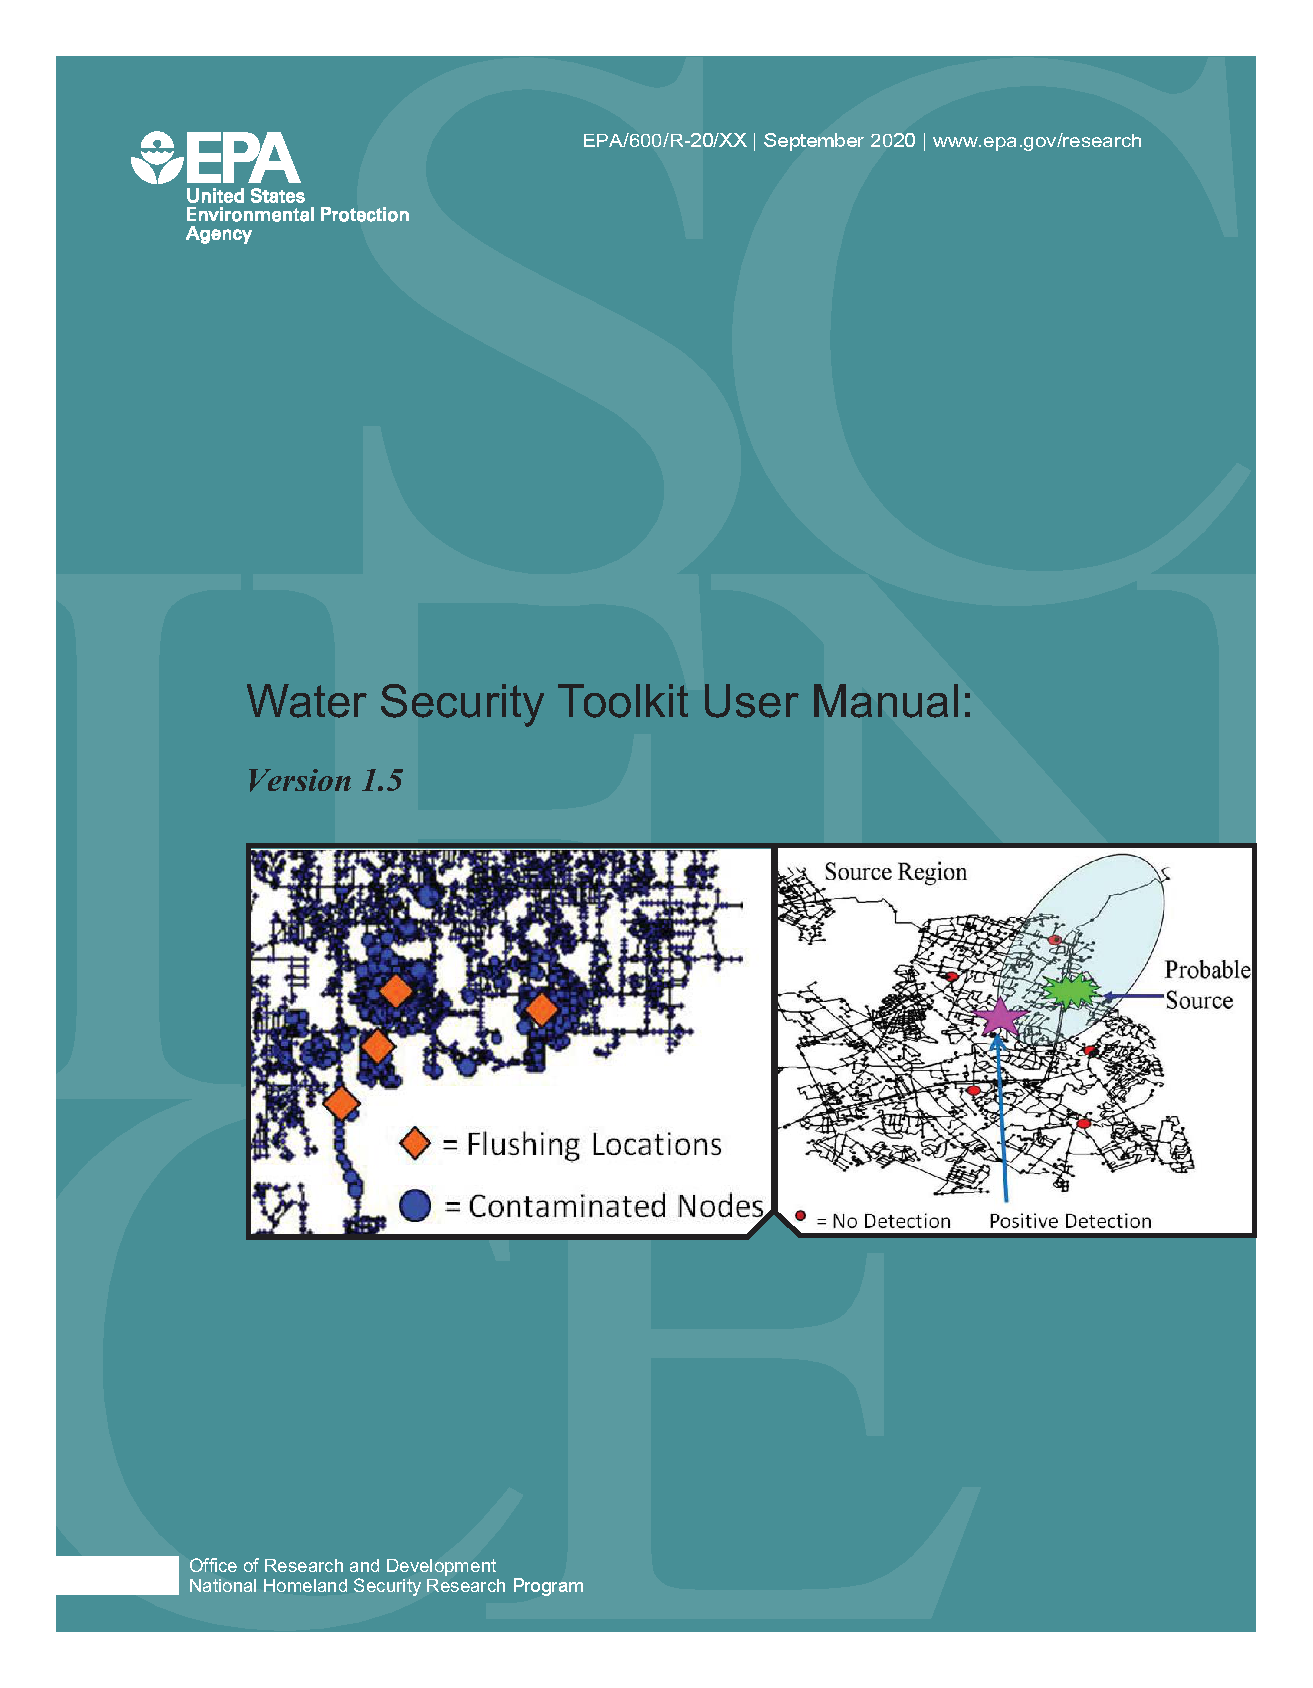
\includepdf[pages={1}]{covers/EPAReport_frontcover_v1-5.pdf}
    \maketitle
  \else
    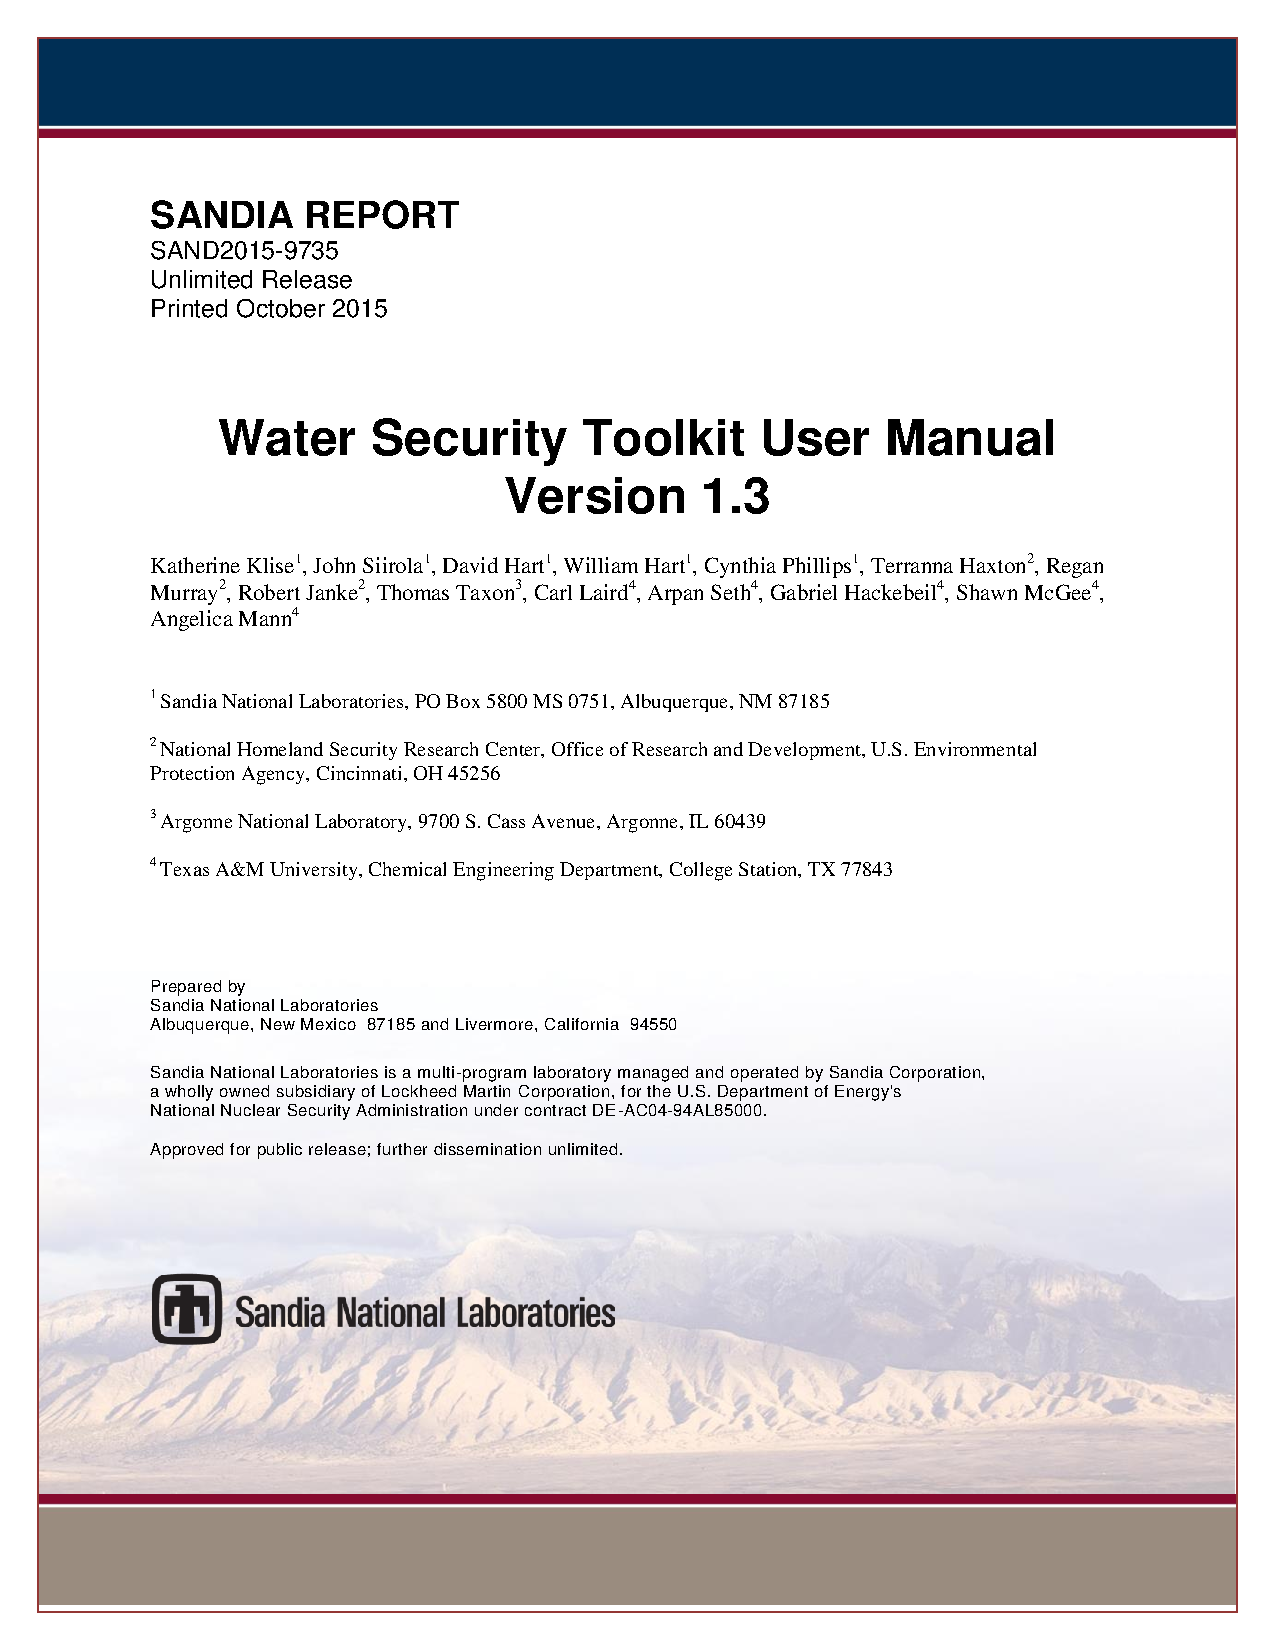
\includepdf[pages={1}]{covers/SANDReport_cover_v1-3.pdf}
    \includepdf[pages={2}]{covers/SANDReport_cover_v1-3.pdf}
    \includepdf[pages={3}]{covers/SANDReport_cover_v1-3.pdf}
  \fi
  
  \clearpage
%  \begin{center}

WATER SECURITY TOOLKIT USER MANUAL:
VERSION 1.5

by 


Katherine Klise, David Hart, John Siirola, William Hart, Cynthia Phillips 
Sandia National Laboratories
Albuquerque, NM 87185


Carl Laird, Arpan Seth, Jose Santiago Rodriguez
Purdue University
West Lafayette, IN 47907


Terranna Haxton, Regan Murray, Robert Janke
U.S. Environmental Protection Agency
Cincinnati, OH 45268


Gabe Hackebeil, Angelica Mann, Shawn McGee
Texas A\&M University
College Station, TX 77843


Thomas Taxon
Argonne National Laboratory
Lemont, IL 60439





Interagency Agreement DW8992450201 






Terranna Haxton
U.S. Environmental Protection Agency Project Officer 
Homeland Security Research Program 
Cincinnati, OH 45268

\end{center}

  
  \pagenumbering{roman}
  \clearpage
  \ifEPAReport
    \chapter*{Disclaimer}
    The U.S. Environmental Protection Agency (EPA) through its Office of 
Research and Development funded and collaborated in the research described 
here under an Interagency Agreement (IA \# DW8992192801 and \# DW8992450201) with the Department 
of Energy's Sandia National Laboratories. It has been subject to the Agency's 
review and has been approved for publication. Note that approval does not 
signify that the contents necessarily reflect the views of the Agency. 
Mention of trade names, products, or services does not convey official 
EPA approval, endorsement, or recommendation.

\bigskip
\bigskip

{\fontseries{b}\selectfont NOTICE:} 
This report was prepared as an account of work sponsored
by an agency of the United States Government. Accordingly, the United
States Government retains a nonexclusive, royalty-free license to
publish or reproduce the published form of this contribution, or allow
others to do so for United States Government purposes. Neither Sandia
Corporation, the United States Government, nor any agency thereof, nor
any of their employees makes any warranty, express or implied, or
assumes any legal liability or responsibility for the accuracy,
completeness, or usefulness of any information, apparatus, product, or
process disclosed, or represents that its use would not infringe
privately-owned rights. Reference herein to any specific commercial
product, process, or service by trade name, trademark, manufacturer,
or otherwise does not necessarily constitute or imply its endorsement,
recommendation, or favoring by Sandia Corporation, the United States
Government, or any agency thereof. The views and opinions expressed
herein do not necessarily state or reflect those of Sandia
Corporation, the United States Government or any agency thereof.

\bigskip
\bigskip

Questions concerning this document or its application should be
addressed to:

\makebox[3.4in][t]{
\begin{minipage}[c][\topheight][t]{3.4in}
Terra Haxton \\
Center for Environmental Solutions and Emergency Response\\
Office of Research and Development\\
U.S. Environmental Protection Agency\\
Cincinnati, OH 45268\\
Haxton.Terra@epamail.epa.gov\\
513-569-7810\\
\end{minipage}
}
\makebox[3.5in][c]{
\begin{minipage}[c][\topheight][t]{3.0in}
\begin{center}

\includegraphics[width=1.2in]{graphics/EPAbwlogo}
\end{center}
\end{minipage}
}

  \fi
  
  %\clearpage
  %\chapter*{Forward}
  %In July of 1970, the White House and Congress worked together to establish 
the United States Environmental Protection Agency (EPA) in response to the 
growing public demand for cleaner water, air, and land. The Agency was assigned 
the daunting task of repairing the damage already done to the natural 
environment and establishing new criteria to guide Americans in making a cleaner 
environment a reality. Since 1970, EPA has worked with federal, state, tribal, 
and local partners to advance its mission to protect human health and the 
environment.

EPA leads the nation's environmental science, research, education, and assessment 
efforts. With more than 17,000 employees across the country, EPA works to 
research, develop, and enforce regulations that implement environmental laws 
enacted by Congress. In recent years, between 40 and 50 percent of EPA's 
enacted budgets have provided direct support through grants to State 
environmental programs. At laboratories located throughout the nation, the 
Agency works to assess environmental conditions and to identify, understand, and 
solve current and future environmental problems. The Agency works through its 
headquarters and regional offices with over 10,000 industries, businesses, 
nonprofit organizations, and state and local governments, on over 40 
voluntary pollution prevention programs and energy conservation efforts. 

Under existing laws and recent Homeland Security Presidential Directives, EPA 
has been called upon to play a vital role in helping to secure the nation 
against foreign and domestic enemies. The National Homeland Security Research 
Center (NHSRC) was formed in 2002 to conduct research in support of EPA's role 
in homeland security. NHSRC research efforts focus on five areas: water 
infrastructure protection, threat and consequence assessment, decontamination 
and consequence management, response capability enhancement, and homeland 
security technology testing and evaluation. EPA is the lead federal agency 
for drinking water and waste water systems and NHSRC is working to reduce 
system vulnerabilities, prevent and prepare for terrorist attacks, minimize 
public health impacts and infrastructure damage, and enhance recovery efforts. 

This \docTitle\ for the Water Security Toolkit software package is published 
and made available by EPA's Office of Research and Development to assist the 
water community in improving the security of our nation's drinking water.

\vspace*{\baselineskip}
\vspace*{\baselineskip}

\begin{tabular}{ll}
 & Gregory Sayles, Ph.D., Acting Director \\

& National Homeland Security Research Center \\
& Office of Research and Development \\
& U. S. Environmental Protection Agency
\end{tabular}


  \clearpage
  \chapter*{License Notice}
  The Water Security Toolkit (WST) v.\wstversion

Copyright \copyright\ 2012-2019 Sandia Corporation. Under the terms of Contract
DE-AC04-94AL85000, there is a non-exclusive license for use of this work
by or on behalf of the U.S. government. 

This software is distributed under the Revised BSD License (see below).  In
addition, WST leverages a variety of third-party software packages, which
have separate licensing policies:

\begin{tabularx}{\textwidth}{p{0.5in}lX}
&\bf Acro & Revised BSD License \\
&\bf argparse & Python Software Foundation License \\
&\bf Boost & Boost Software License \\
&\bf Coopr & Revised BSD License \\
&\bf Coverage & BSD License \\
&\bf Distribute & Python Software Foundation License /  Zope Public License \\
&\bf EPANET 2.00.12 & Public Domain \\
&\bf EPANET-ERD & Revised BSD License \\
&\bf EPANET-MSX & GNU Lesser General Public License (LGPL) v.3 \\
&\bf gcovr & Revised BSD License \\
&\bf GRASP & AT\&T Commercial License for noncommercial use; includes
  \code{randomsample} and \code{sideconstraints} executable files \\
&\bf LZMA SDK & Public Domain \\
&\bf nose & GNU Lesser General Public License (LGPL) v.2.1 \\
&\bf ordereddict & MIT License \\
&\bf pip & MIT License \\
&\bf PLY & BSD License \\
&\bf PyEPANET & Revised BSD License \\
&\bf Pyro & MIT License \\
&\bf PyUtilib & Revised BSD License \\
&\bf PyYAML & MIT License \\
&\bf runpy2 & Python Software Foundation License \\
&\bf setuptools & Python Software Foundation License /  Zope Public License \\
&\bf six & MIT License \\
&\bf TinyXML & zlib License \\
&\bf unittest2 & BSD License \\
&\bf Utilib & Revised BSD License \\
&\bf virtualenv & MIT License \\
&\bf Vol & Common Public License \\
&\bf vpykit & Revised BSD License \\
\end{tabularx}

Additionally, some precompiled WST binary distributions might bundle
other third-party executable files:

\begin{tabularx}{\textwidth}{p{0.5in}lX}
&\bf Coliny & Revised BSD License (part of Acro project) \\
&\bf Dakota & GNU Lesser General Public License (LGPL) v.2.1 \\
&\bf PICO & Revised BSD License (part of Acro project) \\
\end{tabularx}
  
\section*{Revised BSD License}
Redistribution and use in source and binary forms, with or without
modification, are permitted provided that the following conditions are
met:
\begin{itemize}
\item Redistributions of source code must retain the above copyright
  notice, this list of conditions and the following disclaimer.
\item Redistributions in binary form must reproduce the above copyright
  notice, this list of conditions and the following disclaimer in the
  documentation and/or other materials provided with the distribution.
\item Neither the name of Sandia National Laboratories nor Sandia
  Corporation nor the names of its contributors may be used to endorse
  or promote products derived from this software without specific prior
  written permission.
\end{itemize}


\textsc{\bfseries This software is provided by the copyright holders and contributors "as is" and
any express or implied warranties, including, but not limited to, the implied
warranties of merchantability and fitness for a particular purpose are
disclaimed. In no event shall Sandia Corporation be liable for any
direct, indirect, incidental, special, exemplary, or consequential damages
(including, but not limited to, procurement of substitute goods or services;
loss of use, data, or profits; or business interruption) however caused and
on any theory of liability, whether in contract, strict liability, or tort
(including negligence or otherwise) arising in any way out of the use of this
software, even if advised of the possibility of such damage.}

% LocalWords:  WST Sandia Acro argparse Coopr Zope EPANET ERD MSX LGPL gcovr
% LocalWords:  randomsample sideconstraints LZMA SDK ordereddict PyEPANET Pyro
% LocalWords:  PyUtilib PyYAML runpy setuptools TinyXML zlib unittest Utilib
% LocalWords:  virtualenv vpykit precompiled executables Coliny PICO
% LocalWords:  Redistributions


  \clearpage
  \chapter*{Acknowledgements}
  \ifEPAReport
    The U.S. Environmental Protection Agency (EPA) acknowledges the support in the development of the Water Security Toolkit \docTitle , 
and in the development and testing of the Water Security Toolkit software.

The Water Security Toolkit is an extension of the Threat Ensemble Vulnerability 
Assessment-Sensor Placement Optimization Tool (TEVA-SPOT), which was also developed
with funding from the U.S. Environmental Protection Agency through its Office of 
Research and Development (Interagency Agreement \# DW8992192801). EPA would like to 
acknowledge the following individuals for their previous contributions to the development 
of the TEVA-SPOT toolkit software:
Jonathan Berry (Sandia National Laboratories), Erik Boman (Sandia National Laboratories), 
Lee Ann Riesen (Sandia National Laboratories), James Uber (University of Cincinnati), and 
Jean-Paul Watson (Sandia National Laboratories).



  \else
    This work was supported by the U.S. Environmental Protection 
Agency through its Office of Research and Development (Interagency 
Agreement \# DW8992192801). It has been subject to an administrative 
review but does not necessarily reflect the views of the Agency. No official 
endorsement should be inferred. EPA does not endorse the purchase or sale 
of any commercial products or services.

The Water Security Toolkit is an extension of the Threat Ensemble Vulnerability 
Assessment-Sensor Placement Optimization Tool (TEVA-SPOT), which was also developed
with funding from the U.S. Environmental Protection Agency through its Office of 
Research and Development (Interagency Agreement \# DW8992192801).  The authors 
acknowledge the following individuals for their contributions to the development 
of TEVA-SPOT:
Jonathan Berry (Sandia National Laboratories), 
Erik Boman (Sandia National Laboratories),  
Lee Ann Riesen (Sandia National Laboratories), 
James Uber (University of Cincinnati),
and Jean-Paul Watson (Sandia National Laboratories). 
  \fi
  
  \clearpage
  \chapter*{Acronyms}
  \begin{tabularx}{\textwidth}{p{0.5in}lX}
&\bf ATUS & American Time-Use Survey \\
&\bf BLAS & Basic linear algebra sub-routines \\
&\bf CFU & Colony-forming unit \\
&\bf CVAR & Conditional value at risk \\
&\bf CWS & Contamination warning system \\
%&\bf DEC & Detected extent of contamination \\
%&\bf DMC & Detected mass consumed  \\
%&\bf DPD & Detected population dosed \\
%&\bf DPE & Detected population exposed \\
%&\bf DPK & Detected population killed \\
%&\bf DTD & Detected time to detection \\
%&\bf DVC & Detected volume consumed \\
&\bf EA & Evolutionary algorithm \\
&\bf EDS & Event detection system \\
&\bf EPA & U.S. Environmental Protection Agency \\
&\bf EC & Extent of Contamination \\
&\bf ERD & EPANET results database file \\
&\bf GLPK & GNU Linear Programming Kit \\
&\bf GRASP & Greedy randomized adaptive sampling process \\
&\bf HEX & Hexadecimal \\
&\bf HTML & HyperText markup language \\
&\bf INP & EPANET input file \\
&\bf LP & Linear program \\
&\bf MC & Mass consumed  \\
&\bf MILP & Mixed integer linear program \\
&\bf MIP & Mixed integer program \\
&\bf MSX & Multi-species extension for EPANET   \\
&\bf NFD & Number of failed detections  \\
&\bf NS & Number of sensors \\
&\bf NZD & Non-zero demand \\
&\bf ODE & Ordinary differential equation \\
&\bf PD & Population dosed \\
&\bf PDE & Partial differential equation \\
&\bf PE & Population exposed \\
&\bf PK & Population killed \\
&\bf TAI & Threat assessment input file \\
&\bf TCE & Tailed-conditioned expectation \\
&\bf TD & Time to detection \\
% &\bf TEC & Timed extent of contamination \\
&\bf TEVA & Threat ensemble vulnerability assessment \\
&\bf TSB & Tryptic soy broth\\
&\bf TSG & Threat scenario generation file\\
&\bf TSI & Threat simulation input file\\
&\bf VAR & Value at risk \\
&\bf VC & Volume consumed \\
&\bf WST & Water Security Toolkit \\
&\bf YML & YAML configuration file format for WST \\
\end{tabularx}
  
  \clearpage
  \chapter*{Symbols}
  \begin{center}
  \renewcommand\arraystretch{3}
  %\renewcommand\tabcolsep{6pt}
  \begin{tabular}{ | p{2cm} | p{3cm} | p{10cm} | }
    \hline
    \bf Notation &  \bf Definition & \bf Example \\ 
    \hline 
    $\{ , \}$ & set brackets  & $\{1,2,3\}$ means a set containing the values 1,2, and 3. \\ 
    \hline
    $\in$ & is an element of  & $s \in S$ means that $s$ is an element of the set $S$. \\ 
    \hline
    $\forall$ & for all & $s=1$ $\forall$ $s \in S$ means that the statement $s=1$ is true for all $s$ in set $S$. \\ 
    \hline
    $\sum$ & summation & $\sum_{i=1}^{n}{s_i}$ means $s_1 + s_2 + \cdots + s_n$. \\ 
    \hline
    $\setminus$ & set minus & $S \setminus T$ means the set that contains all those elements of $S$ that are not in set $T$. \\ 
    \hline
    $\vert$ & given & $\vert$ is used to define conditional probability.  $P(s|t)$ means the probability of $s$ occurring given that $t$ occurs.  \\ 
    \hline
    $\left|...\right|$ & cardinality & Cardinality of a set is the number of elements of the set.  If set $S = \{2,4,6\}$, then $\left|S\right| = 3$. \\ 
    \hline
  \end{tabular}
\end{center}

  
  \cleardoublepage
  \tableofcontents
  \clearpage
  \listoffigures
  %\listoftables

  %\SANDmain
  \clearpage
  \pagenumbering{arabic}

  \chapter{Introduction}
  An abundant supply of safe, high-quality drinking water is critical to modern industrialized societies. 
At home, water is used for drinking, cooking, washing clothes and bathing. At work, water 
is used to operate restaurants, hospitals and manufacturing plants. In our communities, 
water is used for fighting fires. Consequently, contamination of drinking 
water infrastructure could severely impact the public health and economic vitality of a community. 
The distributed physical layout of drinking water systems makes them inherently vulnerable to a variety 
of incidents, such as terrorist attacks, accidents and even natural disasters. 
The physical destruction of water infrastructure can disrupt water service to communities; 
specifically key facilities such as hospitals, power stations and military installations. Similarly, 
contamination with deadly agents could result in large numbers of illnesses and fatalities.

Since the events of September 11, 2001, water utilities have had increasing concerns about 
the possibility of harm to our water quality due to an accidental or intentional contamination incident within a distribution network. 
The U.S. EPA's Response Protocol Toolbox \citep{ResponseProtocolToolbox} provides recommendations on actions that 
water utilities can take to minimize potential impacts to consumers following a contamination threat or incident. 
Detection and consequence management are major steps in this protocol. EPA has also developed modeling and 
simulation tools to assist in the detection of contamination incidents in water distribution networks. 
The Threat Ensemble Vulnerability Assessment-Sensor Placement Optimization Tool, or TEVA-SPOT \citep{TEVASPOTusermanual}, 
identifies the optimal placement of online water quality monitoring sensors to detect contamination incidents. 
Another EPA developed tool to assist in detection is the CANARY event detection system \citep{CANARY}, 
which analyzes water quality data from sensors and identifies periods of anomalous water quality. 
These tools work together to help form a contamination warning system (CWS). The overall goal of a 
CWS is to detect contamination incidents in time to reduce potential public health and economic consequences. 
The current terminology for a CWS is a water quality surveillance and response system. For more information 
on CWS, see U.S. EPA Water Security Initiative \citep{WSI}.

Should a CWS detect the presence of contamination in a water distribution network, consequence management must be employed. 
Decision-making tools that assist water utilities in evaluating and planning various response strategies 
are needed to support rapid response to contamination incidents. The Water Security Toolkit (WST) is a suite 
of tools that help provide the information necessary to make good decisions 
resulting in the minimization of further human exposure to contaminants, and the maximization of the 
effectiveness of intervention strategies. WST is intended to assist in: 
\begin{itemize}
\item Planning response actions to natural disasters and terrorist attacks, 
\item Developing consequence management plans, 
\item Informing large-scale exercises/training, 
\item Planning response actions to address traditional utility challenges, such as pipe breaks and water quality problems and 
\item Evaluating implications of different response strategies. 
\end{itemize}
For water utilities with hydraulic modeling expertise, WST combined with EPANET-RTX \citep{EPANETRTX,HatchettetalRTX2011,JankeetalRTX2011} 
could use data from CANARY, other sensor stations and field investigations to optimize and 
implement response actions in real-time. 

WST assists in the evaluation of multiple response actions in order to select the most 
beneficial consequence management strategy. It includes hydraulic and water quality 
modeling software and optimization methodologies to identify: (1) sensor locations to detect contamination,
(2) locations in the network in which the contamination was introduced, (3) hydrants to 
remove contaminated water from the distribution system, (4) locations in the network to inject 
decontamination agents to inactivate, remove or destroy contaminants and (5) locations in the network to take grab
sample to confirm contamination or cleanup.

This user manual describes the different components of WST. 
\ifEPAReport
It is also available as a Sandia Report (\citet{WSTSandreport}).
\else
It is also available as an EPA Report (\citet{WSTEPAreport}).
\fi
The manual contains one chapter on each of the water security tools:
\begin{itemize}
\item Contaminant transport
\item Impact assessment
\item Sensor placement
\item Hydrant flushing 
\item Booster placement
\item Source identification
\item Grab sampling
\item Visualization
\end{itemize}
Another chapter discusses advanced topics and provides case studies. 
WST uses YAML format configuration files to supply input parameters to each water security tool.  
Additional information on the YAML format can be found in File Formats Section \ref{formats_yamlFile}.

The contaminant transport simulation, impact assessment and sensor placement optimization tools were all 
developed as part of the TEVA-SPOT Toolkit \citep{TEVASPOTusermanual}. All functionality in TEVA-SPOT has been replicated 
in WST using new, user friendly YAML format configuration files. WST builds upon the simulation and optimization 
framework of TEVA-SPOT and adds several new features. These features were all 
developed to model possible response action plans once a contamination incident has been detected in the system. 
These action plans include redirecting flow by opening hydrants and closing valves, injecting decontaminant 
to inactivate biological agents and using sensor measurements to identify possible source locations.

The main data requirement to use WST is a calibrated water utility network model. Additional input data is 
dependent on the WST application. This includes information on the simulated contamination incident(s) 
(e.g., type, location(s), amount), the impact metric (e.g., extent of contamination, population exposed) 
and the response actions (e.g., flushing hydrants, injecting disinfectant). To optimize a response action, 
WST must be given additional information about the potential locations for water quality sensors, hydrants to flush, valves to close, 
disinfectant booster stations and manual grab samples. The operating characteristics of these different response 
actions are also required, such as the detection limits of the water quality sensors, the rate and duration that 
hydrants can be flushed, the control settings for injecting disinfectant at booster stations and the number of manual 
grab samples that can be taken at the same time. More details on the data requirements are provided 
in the chapter describing each of the specific water security tool. In addition, each chapter has example applications. 
All examples are included with WST and can be found in the examples folder. These examples use simple networks 
and data files that are also distributed with WST. The examples shown in this user manual are all executed on a 
Linux computer, so the CPU time for each example might not be the same on computers with different operating systems. 


  \chapter{Getting Started}
  \label{chap:gettingstarted}
  
This chapter provides information on downloading and
installing WST. WST is an open source toolkit for
modeling and analyzing water distribution systems to minimize the
potential impact of contamination incidents.

\section{Obtaining the Water Security Toolkit}\label{S:getting_wst}

WST is distributed by the EPA in both source and
pre-built binary forms through the World Wide Web at
\url{https://github.com/USEPA/Water-Security-Toolkit}. From the main WST web page,
click the ``Releases'' link. The download page 
has options to download the WST source code as well as pre-built binary
packages for 64-bit Microsoft Windows\textsuperscript{\textregistered} operating system. For most users, 
installing pre-built binary versions of WST is recommended.

Alternatively, the WST source code can be checked out directly from the
master git version control system through
\url{https://github.com/USEPA/Water-Security-Toolkit}. In particular, the
source can be checked out with the git command:
\begin{unknownListing}
git clone https://github.com/USEPA/Water-Security-Toolkit
\end{unknownListing}

\section{Dependencies of the Water Security Toolkit}\label{dependencies}

WST is a collection of Python\texttrademark (Python Software Foundation) and compiled C++ software. It has
dependencies on several third-party software packages. First and
foremost, a Python interpreter must be installed. WST is
currently compatible with Python 2.6 or 2.7. Python 3.x is not 
supported. Python is available from \url{http://python.org/}.

The WST source code and binary distributions bundle several additional
Python packages, including:
\begin{description}[topsep=0pt,parsep=0.5em,itemsep=-0.4em,labelindent=2em,leftmargin=4em]
\item[Coopr]\hfill\\ A collection of open-source optimization-related
  Python packages that support a diverse set of optimization
  capabilities for formulating and analyzing optimization models. Coopr
  in turn bundles several third-party dependency libraries:
  \begin{description}[topsep=0pt,parsep=0.5em,itemsep=-0.4em]
  \item[argparse]\hfill\\ A Python command line argument parsing utility
  \item[coverage]\hfill\\ A Python utility for capturing and reporting
    code coverage
  \item[distribute]\hfill\\ A Python utility for building and installing
    Python packages
  \item[gcovr]\hfill\\ A utility for parsing and reporting GCOV code
    coverage reports
  \item[nose]\hfill\\ A Python test-harness driver
  \item[ordereddict]\hfill\\ A utility that back-ports ordered
    dictionaries to Python 2.6
  \item[pip]\hfill\\ A Python utility for installing Python packages
  \item[ply]\hfill\\ A general parser-lexer
  \item[pyro]\hfill\\ A utility for managing distributed Python execution
  \item[runpy2]\hfill\\ A utility that back-ports runpy functionality to Python 2.4
  \item[setuptools]\hfill\\ A Python utility for building and installing Python packages
  \item[six]\hfill\\ A utility that provides a portable interface to Python 2.x
    and 3.x
  \item[unittest2]\hfill\\ A utility that back-ports unittest functionality from
    Python 2.7 to 2.3-2.6
  \item[virtualenv]\hfill\\ A utility for creating virtual Python environments
  \end{description}
\item[PyUtilib]\hfill\\ A collection of Python utilities, including the testing
  harness used in WST
\item[PyEPANET]\hfill\\ Python wrappers for the EPANET 2.00.12 Programmers Toolkit
\item[PyYAML]\hfill\\ A YAML parser and emitter for Python
\end{description}

WST subcommands can leverage numerous third-party programs that
are not available in the WST zipped file that contains the source code and binary distribution:
\begin{description}[topsep=0pt,parsep=0.5em,itemsep=-0.4em,labelindent=2em,leftmargin=4em]
\item[AMPL]\hfill\\ A commercial algebraic modeling environment, available from
  \url{http://www.ampl.com/}
\item[CBC]\hfill\\ An open-source mixed-integer linear programming
  solver, available from \url{https://github.com/coin-or/Cbc}. The
  COIN Binary Project provides pre-compiled binaries through the
  CoinAll distribution,
  available from \url{https://www.coin-or.org/download/binary/CoinAll}.
\item[CPLEX]\hfill\\ A commercial mixed-integer linear programming solver,
  available from
  \url{https://www.ibm.com/products/ilog-cplex-optimization-studio}
\item[Coliny]\hfill\\ An open-source package that provides algorithms for model
  transformation and black-box optimization, available as 
  part of the Dakota project at \url{http://dakota.sandia.gov/}
\item[Dakota]\hfill\\ An open-source package that provides algorithms for
  black-box optimization, sensitivity analysis, surrogate modeling and
  uncertainty quantification, available from
  \url{http://dakota.sandia.gov/}. For Windows users, the
  6.8 Windows build is recommended. The information on how to download and install Dakota is 
  provided in the \ref{sec.WSTinstall} section.
\item[GLPK]\hfill\\ An open-source mixed-integer linear programming
  solver, available from \url{http://www.gnu.org/software/glpk/}.
  Pre-compiled binary distributions are available as part of most
  UNIX-like operating systems. The GLPK for Windows Project
  provides pre-compiled Windows binaries, available from
  \url{http://winglpk.sourceforge.net/}.
\item[Gurobi]\hfill\\ A commercial mixed-integer linear programming solver,
  available from
  \url{http://www.gurobi.com/}.
%\item[PICO]\hfill\\ An open-source mixed-integer linear programming solver,
%  available as the Acro-pico project from
%  \url{https://software.sandia.gov/trac/acro/}.
\end{description}
Please refer to the individual projects' documentation for licensing,
pricing and installation information.

\section{Installing the Water Security Toolkit Binary Distributions}\label{sec.WSTinstall}

This is the last binary build of the WST software, since it is no longer in active development. The source code is available along with the "NMAKE" files in the appropriate package directory. The build is fragile, since it might require older versions of Python and MSVS runtime libraries. Due to these limitations, the best method to compile and build WST is on a Linux machine. Associated projects under active development include the following: Water Network Tool for Resilience (WNTR) available at \url{https://github.com/USEPA/WNTR}, Chama available at \url{https://github.com/sandialabs/chama} and Pecos available at \url{https://github.com/sandialabs/pecos}.

The following instructions are provided for installing WST on Windows machines.
For the most up-to-date instructions, including updated third-party URLs, please see the Install page on the GitHub site at \url{https://github.com/USEPA/Water-Security-Toolkit}.

\begin{itemize}
\item Download Anaconda 2.7 from \url{https://www.anaconda.com/distribution/#download-section}. Get the ``Anaconda 2.7'' version, not the Anaconda 3.x.

\item Download Dakota/Coliny from \url{https://dakota.sandia.gov/downloads}. Get the ``Windows'', ``6.8'', ``command line only'', ``unsupported'' version (\texttt{dakota-6.8-release-public-Windows.x86.zip}).

\item Download CBC from \url{https://www.coin-or.org/download/binary/CoinAll}. Get the ``Windows 1.7.4'' version build date ``2013-12-26 18:14'' (\texttt{COIN-OR-1.7.4-win32-msvc11.zip}).

\item Download WST. Get the ``Release 2019'' from the ``Releases'' tab (\texttt{wst-2019.zip}).

\item Perform the following steps:
\begin{enumerate}
\item Install Anaconda2 as ``Just Me'' so administrator access is not needed
\item Unzip the \texttt{wst-2019.zip} file into the desired directory 
\item Unzip the \texttt{dakota-6.8-release-public-Windows.x86.zip} file (should create a directory called the same thing, without the .zip extension, in the same directory as the zip file)
\item Copy all the files from the \texttt{dakota-6.8-release-public-Windows.x86/bin} directory into the \texttt{wst-2019/bin} directory
\item Unzip the \texttt{COIN-OR-1.7.4-win-21-msvc11.zip} file (should create a directory called the same thing, without the .zip extension, in the same directory as the zip file)
\item Copy all the files from the \texttt{COIN-OR-1.7.4-win-21-msvc11/win32-msvc11/bin} directory into the \texttt{wst-2019/bin} directory
\item Open an Anaconda Prompt from the ``Start -> Anaconda2'' menu
\item Change directory into the \texttt{wst-2019} directory
\item Type ``install''
\item Change directory into the \texttt{wst-2019/examples} directory
\item Run the examples (e.g., \texttt{wst sp sp\_ex1.yml})

\end{enumerate}
\end{itemize}


\section{Compiling the Water Security Toolkit Source Code}

Compiling WST from the source code is an advanced topic and targeted
only at potential developers. It assumes familiarity with compilers and
build terminology. General users are strongly recommended to use the 
pre-built binary packages whenever possible.  

Compiling WST from the source code uses the Python VirtualEnv package to
set up a virtual Python environment within the WST source code
distribution. The Python components of WST are installed into this
virtual environment to better insulate WST from the other Python installations 
(and vice-versa). The compiled (C++) binary
executable files are installed into a bin directory within the
source code distribution. Currently, WST does not support out-of-source builds.

While WST can be compiled from the source code for Windows and Linux 
operating systems, Windows users are recommended 
to leverage the pre-built binary distributions. WST can be compiled for Linux 
using a 3-step process:
\begin{enumerate}
\item Obtain the WST source code
\item Configure the Python virtual environment
\item Build the C++ executable files
\end{enumerate}

\subsection{Obtaining the Water Security Toolkit Source Code}
The WST source code can either be extracted from a downloaded source zip/tar
archive or checked out directly from the repository using git.
The following directions assume that the source code is in the
wst-\wstversion~directory.

\subsection{Configuring the Python Virtual Environment}
The Python virtual environment is automatically configured by the
\code{setup} command distributed in the top-level directory of the
source code distribution:
\begin{unknownListing}
cd ~/wst-`\wstversion`
./setup
\end{unknownListing}
This configures WST using the system's default Python interpreter and
the bundled versions of the Python dependencies. A different version of Python 
can be used with WST by specifying it explicitly when running
the \code{setup} command:
\begin{unknownListing}
cd ~/wst-`\wstversion`
python2.7 ./setup
\end{unknownListing}

Setup configures the Python virtual environment within the 
wst/python directory (e.g.,/wst-\wstversion/python). The virtual interpreter and the
main \code{wst} command both reside in wst/python/bin directory
(e.g.,/wst-\wstversion/python/bin/wst). If only a single virtual environment 
is going to be on the machine, adding the wst/python/bin directory to 
the system PATH variable is recommended. Alternatively, 
the \code{lbin} and \code{lpython} commands (installed
into wst/python/bin) can be used to correctly locate local binaries and
the local virtual python interpreter. To run the \code{wst} command from anywhere
under the main WST directory, use the \code{lbin wst} command.
Similarly, to run the local python (virtual environment) interpreter,
use the \code{lpython} command. It is safe to copy both \code{lbin}
and \code{lpython} to other directories (e.g.,/bin).

After the installation of the core functionality of the python environments
a couple of installations are required. 

\begin{unknownListing}
pip install numpy
pip install texttable
pip install matplotlib
\end{unknownListing}

\subsection{Building the C++ Executable Files}

WST relies on the GNU Autotools to manage the build process for compiled
executables. In particular, Autoconf version 2.60 or
newer must be installed on the system along with a relatively new C++ compiler
and linker (e.g., gcc >= 3.4). The build process follows the normal
\code{autoreconf -- configure -- make} sequence:
\begin{unknownListing}
cd ~/wst-`\wstversion`
./setup
autoreconf -v -i -f
./configure
make
\end{unknownListing}
It is not recommended to use the \code{make install} command. The
resulting compiled binaries reside in wst/bin, and are easily
accessed from anywhere under the main WST directory using the
\code{lbin} command.

This process could be simplified by using the main \code{setup} command:
\begin{unknownListing}
cd ~/wst-`\wstversion`
./setup build
\end{unknownListing}


\section{Basic Usage of the Water Security Toolkit}\label{usage}

The main command line structure to execute a WST subcommand is the following:
\begin{unknownListing}
wst SUBCOMMAND <configfile>
\end{unknownListing}
where \code{SUBCOMMAND} is the one of subcommands available under the 
\code{wst} command and \code{configfile} is the configuration file associated 
with the specified subcommand. The subcommands include the following:
\begin{itemize}
\item \code{tevasim}
\item \code{sim2Impact}
\item \code{sp} 
\item \code{flushing} 
\item \code{booster\_msx}
\item \code{booster\_mip}
\item \code{inversion}
\item \code{grabsample}
\item \code{visualization}
\end{itemize}
Each subcommand is described in more detail in Chapters \ref{chap:tevasim} 
through \ref{chap:visualization}.
 
In addition, the \code{---help} option prints information 
about the different subcommand options available. 
\begin{unknownListing}
wst --help
\end{unknownListing}

Each subcommand has the option to generate a template configuration file by using 
the following command line:
\begin{unknownListing}
wst SUBCOMMAND --template <configfile>
\end{unknownListing}
where \code{configfile} is the name of the template configuration file created for 
the specified \code{SUBCOMMAND}.

\section{Verifying Installation of the Water Security Toolkit}\label{simple_example}

An example using one of the WST subcommands can be used to verify 
the proper installation of WST. This example uses the WST subcommand \code{tevasim}, 
which is documented in Chapter \ref{chap:tevasim}.

\begin{enumerate}
  \item A template configuration file for the \code{tevasim} subcommand 
  can be generated using the following command line, in which verify-wst.yml 
  is the template configuration file to be created:
    \begin{unknownListing}
wst tevasim --template verify-wst.yml
\end{unknownListing}
    This example assumes that the wst/bin directory was added to the PATH variable. 
	If the path was not modified, the \code{wst} command would be replaced with the full 
	path to the main WST script (e.g., C:\textbackslash wst-\wstversion\textbackslash bin\textbackslash wst)
	in this and all subsequent commands.
  \item The EPANET input file for the example network (Net3.inp) needs to be copied from the
    wst/examples/Net3 directory to the current working directory, since it is 
	the network file referenced in the generated template file. On Windows (assuming WST 
	is installed to C:\textbackslash wst-\wstversion), the command line to copy this file is the following:
    \begin{unknownListing}
copy C:\wst-`\wstversion`\examples\Net3\Net3.inp
\end{unknownListing}
    On Linux (assuming WST is installed to \textasciitilde/wst-\wstversion), the command line 
	to copy this file is the following:
    \begin{unknownListing}
cp ~/wst-`\wstversion`/examples/Net3/Net3.inp
\end{unknownListing}
  \item The \code{tevasim} subcommand using this example is executed with the following 
  command line:
    \begin{unknownListing}
wst tevasim verify-wst.yml
\end{unknownListing}
    This runs the \code{tevasim} subcommand and produces the output shown in Figure \ref{fig:tevasim_getting started}
\end{enumerate}

\begin{figure}[h]
\unknownInputListing{examples/tevasim/template_screen.txt}{}{1}{11}
\caption{The \code{tevasim} template screen output.}
\label{fig:tevasim_getting started}
\end{figure}


\section{Uninstalling the Water Security Toolkit}

As WST does not rely on a formal installer, uninstalling WST only requires
deleting the main WST directory (regardless if the 
pre-built binaries were installed or WST was built from the source code). 
If the wst/bin and/or wst/python/bin directories were added to the system
PATH variable, these entries should be removed also.

% LocalWords:  WST Sandia wst exe tevasim yml inp TEVA basicstyle
% LocalWords:  lineskip EPANET



  %\part*{}
  %\addcontentsline{toc}{part}{WST Subcommands}

  \chapter{Contaminant Transport}
  \label{chap:tevasim}
  This chapter describes how to simulate contamination incidents in a water distribution network, 
which is one of the first steps before designing a water quality sensor network or evaluating
response actions to a contamination incident. The \code{tevasim} subcommand simulates 
the hydraulics and contaminant transport within a water distribution network model, which 
consists of pipe, node, pump, valve, storage tank and reservoir components. 
The \code{tevasim} subcommand uses the hydraulic engine from EPANET 2.00.12 to solve the flow 
continuity and headloss equations \citep{EPANETusermanual}. Water quality simulations are calculated
using either EPANET 2.00.12 \citep{EPANETusermanual}, EPANET-MSX \citep{ShaUbeRos11}
or Merlion \citep{Merlion12}. To increase efficiency when simulating a large ensemble 
of contamination incidents, the \code{tevasim} subcommand uses a single hydraulic simulation 
to simulate an ensemble of water quality simulations. 
A flowchart representation of the \code{tevasim} subcommand is shown in Figure \ref{fig:tevasim-flowchart}. 
The utility network model is defined by an EPANET compatible network model (INP format) in WST. 
The simulation input is supplied through the \code{tevasim} WST configuration file.

\begin{figure}[h]
  \centering
  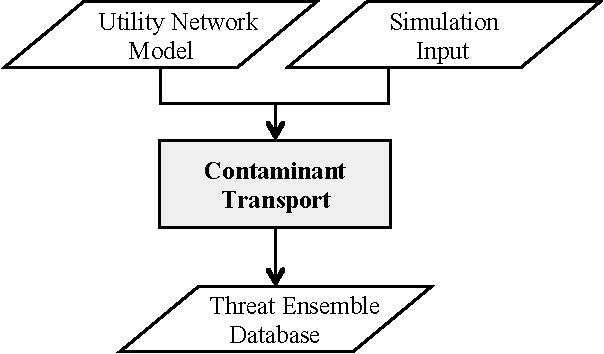
\includegraphics[scale=0.80]{graphics/tevasim_flowchart.pdf}
  \caption{Contaminant transport simulation flowchart.}
  \label{fig:tevasim-flowchart}
\end{figure}

\section{Hydraulic and Water Quality Analysis}
Three water quality simulators, EPANET, EPANET-MSX and Merlion, can be used within WST. These 
simulators are explained in more detail in the following subsections.
\subsection{EPANET and EPANET-MSX}\label{epanet}
EPANET performs extended-period simulation of the hydraulic and water quality 
behavior within pressurized pipe networks. These models can evaluate the 
expected flow in water distribution systems, and model the transport of 
contaminants and related chemical interactions. The multi-species extension, 
EPANET-MSX, is also included in WST to simulate contamination incidents 
using multi-species reactions. Any reaction dynamics between chemical and/or 
biological species (e.g., chemical-chemical, chemical-biological or
biological-biological) can be modeled and simulated using EPANET-MSX. 
EPANET-MSX can be used in sensor network design (\code{sp} subcommand) and 
booster station placement (\code{booster\_msx} subcommand). More specifics 
on these applications can be found in Chapters \ref{chap:sp} and \ref{chap:booster}. 
Additional information on EPANET can be found at 
\url{https://www.epa.gov/water-research/epanet}
and in the EPANET 2.00.12 user manual \citep{EPANETusermanual}. Additional information 
on EPANET-MSX can be found in the EPANET-MSX user manual \citep{ShaUbeRos11}.

\subsection{Merlion}\label{merlion}
The \code{tevasim} subcommand also includes a water quality modeling framework
called Merlion. Unlike EPANET, Merlion does not model bulk or wall
reactions. Given hydraulic information from simulation packages like
EPANET or experimental data, Merlion models the transport of a substance
as it spreads through the water distribution system based on the network
dynamic flow patterns. Merlion first formulates a linear water quality model 
with explicit all-to-all mapping (inputs include injections at all possible nodes 
and time steps, and outputs include concentrations at all possible nodes and 
time steps). This model is then used for forward
tracing simulations by first specifying the injection profile and
then solving the system for the network concentration profile. The linear model 
can also be embedded within other numerical
applications or for analysis in many security applications. Using Merlion in the   
\code{tevasim} subcommand can be faster for multi-scenario simulations; however,
it is also more memory intensive. Merlion can also be used to  
identify booster station locations, contaminant source injection locations 
and manual grab sample locations. More specifics about these applications are in Chapters 
\ref{chap:booster}, \ref{chap:inversion} and \ref{chap:grabsample}. 
More information on Merlion can be found in Section \ref{appendixMerlion} and \citet{Merlion12}.

\section{Contaminant Transport Scenarios}\label{sec:scenarios}
Contaminant transport scenarios can be defined directly in a WST configuration file
or by using a TSI or TSG file. These options are set in the scenario
block of the configuration file for all of the WST subcommands that require scenarios.

The recommended approach is to define the contamination transport scenarios directly in 
the scenario block of the WST configuration file. The options that must be set are 
the location, type, strength, species (required only for EPANET-MSX) 
and start and end times for the contamination scenarios. 
The injection location can be specified by a list of EPANET node IDs, 
or by the key words NZD (non-zero demand nodes) or ALL (all nodes) to create an ensemble of contaminant scenarios. 
The injection type can be CONCEN, MASS, FLOWPACED or SETPOINT as defined in the EPANET user manual\citep{EPANETusermanual}.  
CONCEN represents the concentration of an external source entering a node and 
applies only when the node has a net negative demand (i.e., flows into the network). 
MASS, FLOWPACED and SETPOINT represent booster sources, 
where a contaminant is injected directly into the network regardless of nodal demand.
A MASS source type adds a fixed mass flow to that resulting from inflow to the node, while 
a FLOWPACED booster adds a fixed concentration to the resultant inflow concentration at the node.
A SETPOINT booster fixes the concentration leaving the node as long as the 
inflow concentration was below the setpoint.
The strength of a MASS source is in units of mass flow per minute, while
CONCEN, FLOWPACED and SETPOINT sources are in units of concentration (mass per volume). 
The configuration file defines injection time in minutes and strength in mg/L or mg/min 
depending on the injection type.

Alternatively, the contamination transport scenarios can be defined using a TSI or TSG file. 
Each line of a TSI file specifies a single contaminant scenario by listing the 
injection location, type, species (required only for EPANET-MSX), strength and time frame. Each scenario can include 
multiple injection locations and multiple injection species with unique injection strengths and
time frames. This format allows for the greatest flexibility in combined scenario options.  
For more detail on the TSI file, see File Formats Section \ref{formats_tsiFile}.

The TSG file is a short hand format of the more detailed TSI file. 
Multiple injection locations can be specified on a single line. All permutations of the 
combined locations are used to create multiple scenarios. Each line of the TSG file is limited 
to a single injection species and time frame. For more detail on the TSG file, see File Formats Section \ref{formats_tsgFile}.
The TSI and TSG files specify the injection time frame in seconds (which is different than 
the units specified for the start and end times in the configuration file) and 
the strength units depend on the INP network model file units. 

Specifying a TSI file overrides the TSG file, as well as the location, 
type, strength, species, start time and end time options specified in the WST configuration file.  
Specifying a TSG file overrides the location, type, strength, species, start time and 
end time options specified in the WST configuration file.   

\section{\code{tevasim} Subcommand}

The \code{tevasim} subcommand is executed using the following command line:
\begin{unknownListing}
wst tevasim <configfile> 
\end{unknownListing}
where \code{configfile} is a WST configuration file in the YAML format.  

The \code{---help} option prints information about this subcommand, such as usage,
arguments and a brief description:

\begin{unknownListing}
wst tevasim --help
\end{unknownListing}

\subsection{Configuration File}

The \code{tevasim} subcommand generates a template configuration file using the following command line:

\begin{unknownListing}
wst tevasim --template <configfile>
\end{unknownListing}

The \code{tevasim} WST template configuration file is shown in Figure \ref{fig:tevasim_template}. Brief descriptions 
of the options are included in the template after the \# sign.  

\begin{figure}[h]
  \unknownInputListing{examples/tevasim_config.yml}{}{1}{21}
  \caption{The \code{tevasim} configuration template file.}
  \label{fig:tevasim_template}
\end{figure}
  
\subsection{Configuration Options}

Full descriptions of the WST configuration options used by the \code{tevasim} subcommand are listed below.
\begin{description}[topsep=0pt,parsep=0.5em,itemsep=-0.4em]
  \item[{network}]\hfill
  \begin{description}[topsep=0pt,parsep=0.5em,itemsep=-0.4em]
    \item[{epanet file}]\hfill
\\ The name of the EPANET 2.00.12 input (INP) file that defines the water distribution
                network model.
                
                Required input.
  \end{description}
  \item[{scenario}]\hfill
  \begin{description}[topsep=0pt,parsep=0.5em,itemsep=-0.4em]
    \item[{location}]\hfill
\\A list that describes the injection locations for the contamination scenarios.
                The options are: (1) ALL, which denotes all nodes (excluding tanks and reservoirs)
                as contamination injection locations; (2) NZD, which denotes all nodes with
                non-zero demands as contamination injection locations; or (3) an EPANET node ID, 
                which identifies a node as the contamination injection location. This allows 
                for an easy specification of single or multiple contamination scenarios.
                
                Required input unless a TSG or TSI file is specified.
    \item[{type}]\hfill
\\The injection type for the contamination scenarios. The options are MASS, CONCEN, FLOWPACED or SETPOINT. 
                See the EPANET 2.00.12 user manual for additional information about source types \citep{EPANETusermanual}.
                
                Required input unless a TSG or TSI file is specified.
    \item[{strength}]\hfill
\\The amount of contaminant injected into the network for the contamination scenarios.  
                If the type option is MASS, then the units for the strength are in mg/min. 
                If the type option is CONCEN, FLOWPACED or SETPOINT, then units are in mg/L.
                
                Required input unless a TSG or TSI file is specified.
    \item[{species}]\hfill
\\The name of the contaminant species injected into the network. This is the name of a single species. 
                It is required when using EPANET-MSX, since multiple species might be simulated, but
                only one is injected into the network. For cases where multiple contaminants are injected,
                a TSI file must be used.
                
                Required input for EPANET-MSX unless a TSG or TSI file is specified.
    \item[{start time}]\hfill
\\The injection start time that defines when the contaminant injection begins. 
                The time is given in minutes and is measured from the start of the simulation. 
                For example, a value of 60 represents an injection that starts at hour 1 of the simulation.
                
                Required input unless a TSG or TSI file is specified.
    \item[{end time}]\hfill
\\The injection end time that defines when the contaminant injection stops.				
                The time is given in minutes and is measured from the start of the simulation.
                For example, a value of 120 represents an injection that ends at hour 2 of the simulation.
                
                Required input unless a TSG or TSI file is specified.
    \item[{tsg file}]\hfill
\\The name of the TSG scenario file that defines the ensemble of contamination
                scenarios to be simulated. Specifying a TSG file will
                override the location, type, strength, species and start and end times options specified in
                the WST configuration file. The TSG file format is documented in File Formats Section \ref{formats_tsgFile}.
                
                Optional input.
    \item[{tsi file}]\hfill
\\The name of the TSI scenario file that defines the ensemble of contamination
                scenarios to be simulated. Specifying a TSI file will
                override the TSG file, as well as the location, type, strength, species and start and end time options specified in
                the WST configuration file. The TSI file format is documented in File Formats Section \ref{formats_tsiFile}.
                
                Optional input.
    \item[{signals}]\hfill
\\Name of file or directory with information to generate 
                or load signals. If a file is provided the list of INP-TSG tuples
                 will be simulated and the information stored in signals files. If
                a directory with the signals files is specified, the signal files will
                be read and loaded in memory. This input is only valid for the uq
                subcommand and the grabsample subcommand with probability based formulations.

                Optional input.
    \item[{msx file}]\hfill
\\The name of the EPANET-MSX multi-species file that defines the multi-species reactions to
                be simulated using EPANET-MSX.
                
                Required input for EPANET-MSX.
    \item[{msx species}]\hfill
\\The name of the MSX species whose concentration profile will be saved by the EPANET-MSX simulation
                and used for later calculations.
                
                Required input for EPANET-MSX.
    \item[{merlion}]\hfill
\\A flag to indicate if the Merlion water quality
                simulator should be used. The options are true or false. 
                If an MSX file is provided, EPANET-MSX will be used.
                
                Required input, default = false.
  \end{description}
  \item[{configure}]\hfill
  \begin{description}[topsep=0pt,parsep=0.5em,itemsep=-0.4em]
    \item[{output prefix}]\hfill
\\The prefix used for all output files.
                
                Required input.
    \item[{output directory}]\hfill
      \\The output directory to store the results.
    \item[{debug}]\hfill
\\The debugging level (0 or 1) that indicates the amount of debugging 
                information printed to the screen, log file and output yml file. 
                
                Optional input, default = 0 (lowest level).
  \end{description}
\end{description}


\subsection{Subcommand Output}

The \code{tevasim} subcommand creates 
two output files, one is in the YAML file format and the other is a log file.
The YAML file is called <output prefix>tevasim\_output.yml  
and the log file is <output prefix>tevasim\_output.log. The YAML file 
contains the name of the EPANET report file, the name of the binary ERD database file, 
the run date and the CPU time. 
The EPANET report file and binary ERD database files are described below.
The log file contains basic debugging information.

\begin{itemize}
\item EPANET report: This file provides information on the EPANET simulations. 
The EPANET report file format is described in Appendix C.3 of the EPANET 2.00.12 Users Manual \citep{EPANETusermanual}.
\item ERD database: The database contains the simulation results, 
and is stored in four files: header file, index file, hydraulics file and a water 
quality file. The ERD database format is described in \citet{ERDusermanual}. This files is not
intended to be read by users but rather is read by other WST subcommands.
\end{itemize}

\section{Contaminant Transport Examples}\label{tevasim_example}

An EPANET network model (INP format) and a configuration file are required to 
run the \code{tevasim} subcommand.  

The \code{tevasim} template configuration file uses the EPANET Example Network 3 (Net3.inp).  
The network is shown in Figure \ref{fig:Net3}. 
Net3 contains 92 junctions, 2 reservoirs and 3 tanks. This network has 59 non-zero 
demand (NZD) nodes. The network file is setup to run a 
48-hour hydraulic and water quality simulation. A 1-hour 
hydraulic time step and 5-minute water quality time step are used.

\begin{figure}[h]
  \centering
  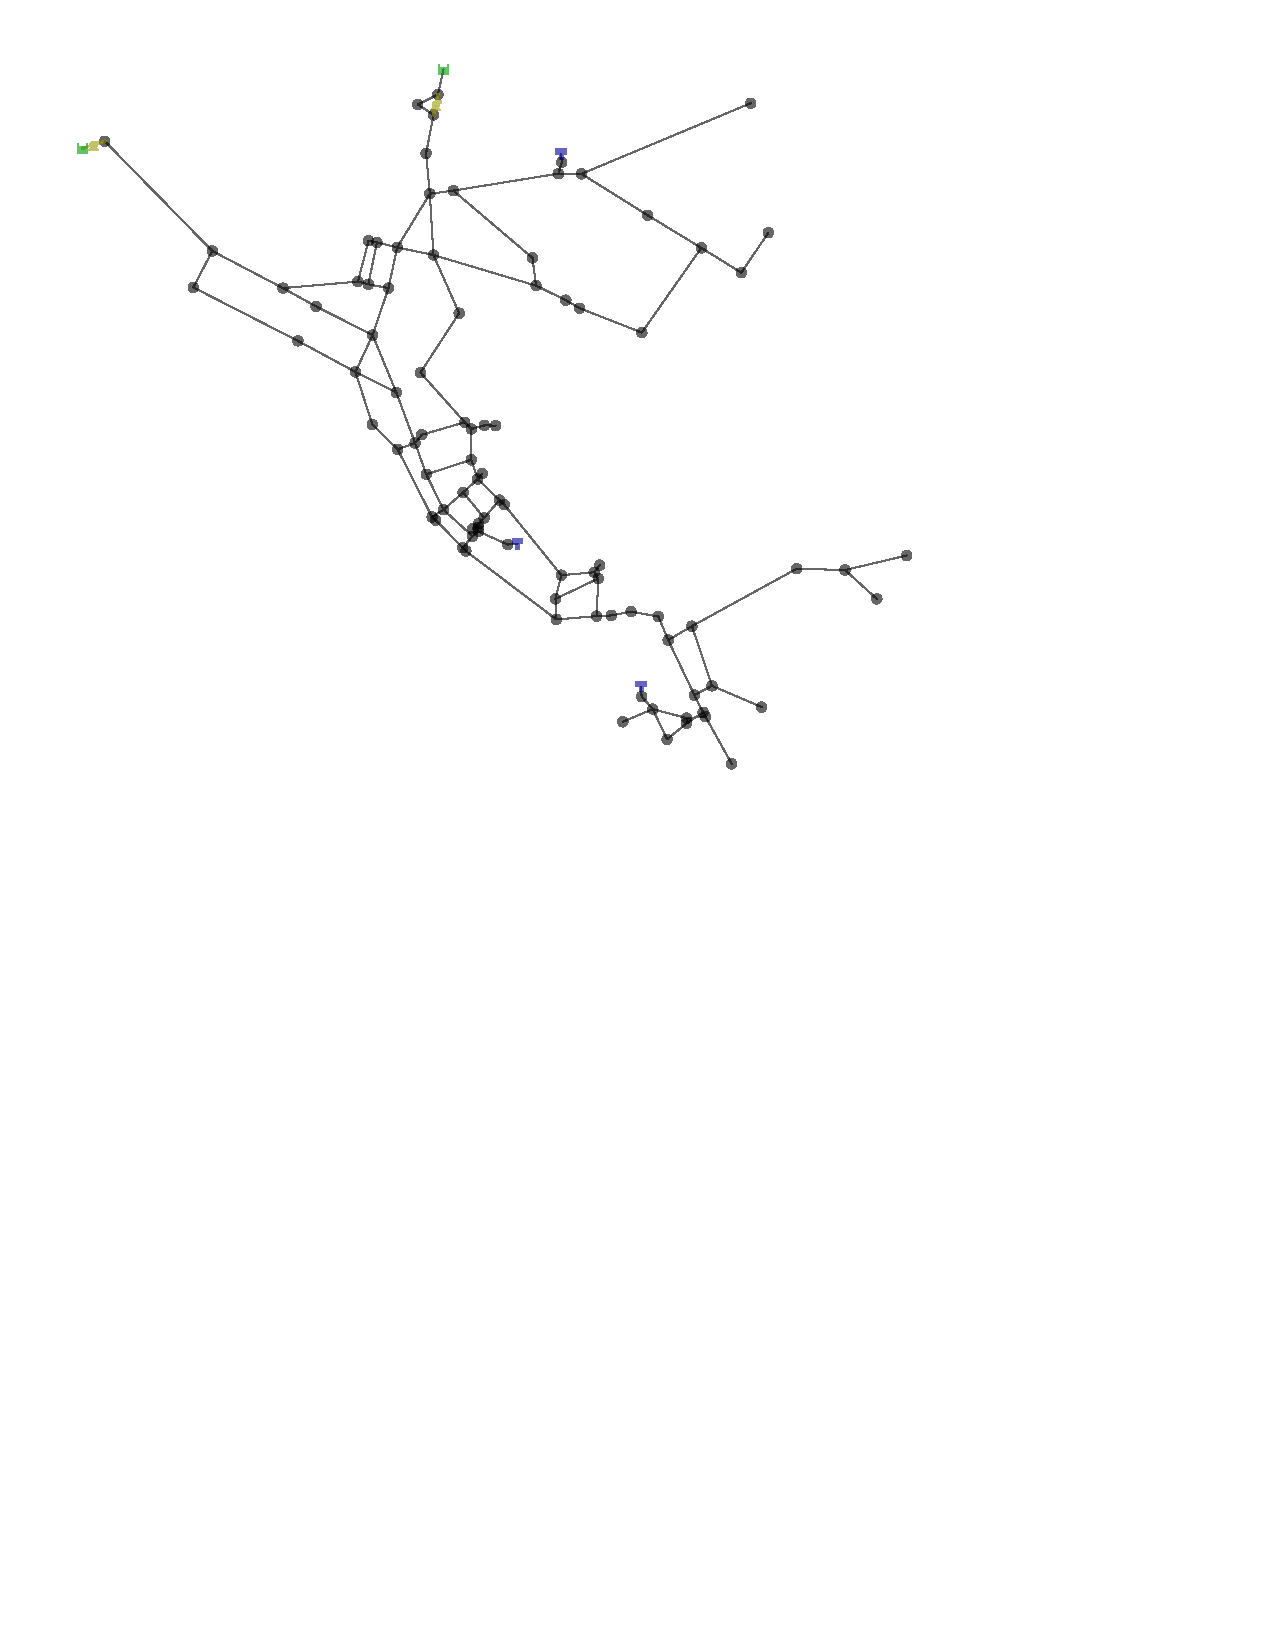
\includegraphics[scale=0.80]{graphics/Net3.pdf}
  \caption{Layout of the EPANET Example Network 3.}
  \label{fig:Net3}
\end{figure}

The scenario ensemble in the \code{tevasim} template configuration file defines 
a contaminant injection from each NZD node, with a MASS injection of 100 mg/L, starting 
at time 0 and injecting for 24 hours (1440 minutes).  

To define scenarios that start and stop at multiple times, a TSG file can be 
used to define the scenario set. Figure \ref{fig:Net3tsg} shows the example TSG file, Net3.tsg, in which the 
contamination scenarios are injected at all NZD nodes 
starting at 12 am, 6 am, 12 pm and 6 pm for a total of 236 scenarios. Each injection 
lasts 24 hours and injects a contaminant at 100 mg/L.

\begin{figure}[h!]
  \unknownInputListing{../../examples/Net3/Net3.tsg}{}{1}{8}
  \caption{Example TSG contamination scenario file.}
  \label{fig:Net3tsg}
\end{figure}

\subsection{Example 1}

The first example uses the Net3.inp network file, the contamination scenario set defined by Net3.tsg 
and the Merlion water quality model. The configuration file, tevasim\_ex1.yml, for this example is shown in Figure \ref{fig:tevasim_ex1}.  

\begin{figure}[h!]
  \unknownInputListing{../../examples/tevasim_ex1.yml}{}{1}{8}
  \caption{The \code{tevasim} configuration file for example 1.}
  \label{fig:tevasim_ex1}
\end{figure}

The example can be executed using the following command line:

\begin{unknownListing}
wst tevasim tevasim_ex1.yml
\end{unknownListing}

\FloatBarrier 
\subsection{Example 2}

The second example uses EPANET-MSX to simulate the transport of multiple contaminants. 
For a multi-species simulation, a MSX file and the MSX species must be added to the 
\code{tevasim} configuration file. The MSX species is the species whose concentration profile
will be saved by EPANET-MSX to be used for future calculations. The MSX species can be different
than the species which is injected into the network. The configuration file, tevasim\_ex2.yml, 
for this example is shown in Figure \ref{fig:tevasim_ex2}. The example uses the Net3.inp network file 
and the MSX file, Net3\_EColi\_TSB.msx, which simulates the reaction dynamics between
$Escherichia~coli$, chlorine and a tryptic soy broth (TSB), a nutrient broth that helps to grow bacteria. 
For more information about this specific reaction dynamics, see the $E.~coli$-TSB model 
described in \citet{MurrayAdcockRiceUberHatchett11}. In this example, both the species and MSX species are the
same.

\begin{figure}[h]
  \unknownInputListing{../../examples/tevasim_ex2.yml}{}{1}{17}
  \caption{The \code{tevasim} configuration file for example 2.}
  \label{fig:tevasim_ex2}
\end{figure}

The example can be executed using the following command line:

\begin{unknownListing}
wst tevasim tevasim_ex2.yml
\end{unknownListing}

To simulate the simultaneous injection of two species, a TSI file is needed. For example, the TSI file, 
Net3\_EColi\_TSB.tsi, defines the simultaneous injection of $E.~coli$ and TSB at multiple locations 
within Net 3. The TSI file contains explicit injections for the 59 NZD nodes used in example 1, with 
four species injected per node.


  \chapter{Impact Assessment}
  \label{chap:sim2Impact}
  The potential consequences of individual contamination scenarios can be quantified 
using the results from the contaminant transport simulations and a variety of impact 
assessment metrics. The \code{sim2Impact} subcommand performs impact assessments 
using the output threat ensemble database (ERD) from the \code{tevasim} subcommand. This analysis
provides all necessary network statistics for sensor network design (described 
in Chapter \ref{chap:sp}) as well as response actions, such as flushing hydrants and 
boosting disinfectant (described in Chapters \ref{chap:flush} and \ref{chap:booster}, respectively). 

A flowchart representation of the \code{sim2Impact} subcommand is shown in Figure \ref{fig:sim2Impact-flowchart}. 
The threat ensemble database (ERD) is the output from the \code{tevasim} subcommand and is 
required input for the \code{sim2Impact} subcommand. The consequences input parameters are supplied 
through the \code{sim2Impact} WST configuration file. Additional input data that describes 
the exposure and dose response models of a particular contaminant is required if a human health 
impact metric is used. These models are defined by parameters listed in a threat assessment input (TAI) file. 
More details on the TAI file are provided in the File Formats Section \ref{formats_taiFile}.  

\begin{figure}[h]
  \centering
  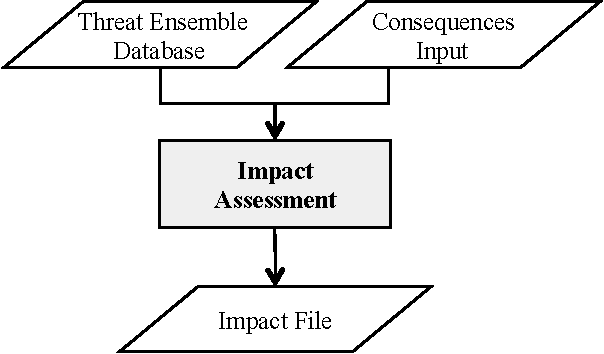
\includegraphics[scale=0.8]{graphics/sim2Impact_flowchart.pdf}
  \caption{Impact assessment flowchart.}
  \label{fig:sim2Impact-flowchart}
\end{figure}

Several impact metrics are included in the \code{sim2Impact} subcommand to reflect different 
criteria that decision makers could use in sensor network design or response actions. These metrics include:  
population dosed (PD), 
population exposed (PE),
population killed (PK), 
extent of contamination (EC),
%timed extent of contamination (TEC),
mass consumed (MC),  
volume consumed (VC), 
time to detection (TD) and
number of failed detections (NFD).
The equations used to compute the impact metrics are listed 
in Section \ref{impact_measures}.
Impact metrics are calculated at discrete time steps for a given 
contamination scenario. 
The discrete time steps are defined by the reporting time step and the duration of the water quality simulation.

Human health impacts (PD, PE and PK) can be estimated by combining 
the water quality simulations with exposure models. 
Contaminant-specific data are needed to accurately estimate the health endpoints. 
For many contaminants, reliable data are lacking, and the ensuing uncertainty 
in the results must be understood. More information on the human health impacts is 
provided in Section \ref{public_health_impacts}.

\section{Impact Metrics}\label{impact_measures}
Impact assessment results are calculated and stored in an impact file. 
This file is not typically read by a WST user, rather it is read by a sensor or 
response optimization routine. For each contamination scenario, the impact file 
contains a list of all the locations (nodes) in the network where a sensor might detect 
contamination from a specific scenario. Nodes that do not detect 
contamination are not included in the impact file for that specific scenario.
For each node that detects contamination, the impact file contains the detection time 
and consequence at that time, as measured by one of the impact metrics. 

The impact file is used as input for sensor placement optimization and during the 
optimization process of response actions, such as flushing hydrants and boosting disinfectant.   
When calculating impacts, a detection threshold can be specified such that contaminants 
are only detected above a specified concentration 
limit (the default limit is zero). Second, a response time can be specified in the \code{sim2Impact} configuration file, 
which accounts for the time needed to verify the presence of contamination 
(e.g., by field investigation), inform the public and/or initiate flushing, booster disinfection, 
or other response action (the default response time is zero). 
The contamination impact is computed at the time when the 
response has been initiated (the detection time plus response time), which is called 
the effective response time. Finally, a detection confidence can be defined, 
which specifies the number of sensors that must detect contamination from any given scenario 
before it is considered to be detected, at which time the impacts 
are calculated (the default is 1 sensor). 

The impact file contains four columns of information: 
\begin{itemize}
\item Column 1 contains the contamination scenario number, $a$
\item Column 2 contains the node location where contamination was detected, $i$
\item Column 3 contains the effective response time in minutes, $T'_i$
\item Column 4 contains the impact at the effective response time as measured by a specified metric, $d_{a,i}$
\end{itemize}
The impact file is documented in the File Formats Section \ref{formats_impactFile}.
The impact metric, $d_{a,i}$, is used directly in the sensor placement formulation (Equation \ref{eqn:eSP}),
the flushing formulation and the booster formulation.

The effective response time at node $i$, $T'_i$, is calculated using the following equation:
\begin{equation}
T'_i = \min{(t : \left|C_{n,t}>\textrm{detection limit}\right| \geq\textrm{detection confidence})}\Delta{T} + \textrm{response time}
\end{equation}
where $C_{n,t}$ is the contaminant concentration at node $n$ at time step $t$ for every node and time step in the water quality simulation.  
The concentration is typically expressed in units of milligrams per liter (mg/L). 
Concentration could also be a count of cells for a biological contaminant, where the units are cells/L or CFU/L (colony forming units/L).
The length of the reporting time step is denoted as $\Delta{T}$ and has units of time.
For detection, the concentration must be above the detection limit, and the number of detections must be above the detection confidence.
(Note $\left|C_{n,t}>\textrm{detection limit}\right|$ is the number of node, 
time step pairs where contaminant was detected above the detection limit, this includes detection at node $i$).

In the impact file, the impact at the end of the simulation time is included for each contamination scenario. 
Essentially, this is the impact if contamination was not detected at any node location, 
and is often referred to as the dummy sensor location.  The dummy sensor location is not a physical location in the network. For this entry, $i$ is set to -1, 
$T'_i$ is the time at the end of the water quality simulation and $d_{a,i}$ is 
the impact at the end of the simulation.

The impact, $d_{a,i}$, can be computed using one of the following metrics:
PD, PE, PK, EC, MC, VC, TD and NFD.
These metrics are defined in the following equations.  
In the equations, the effective response time step for node $i$, $t'_i$, equals $T'_i/\Delta{T}$, and
subscripts $n$, $t$ and $p$ are used to reference a specific node, time step and person, respectively.

\begin{itemize}

\item $\mathrm{PD}_{a,i}$, population dosed, is the total number of individuals that received a cumulative dose of contaminant 
above a specified threshold for scenario $a$ when contamination is detected at node $i$:

\begin{equation}
\mathrm{PD}_{a,i}=\sum_{n=1}^{N}\sum_{p=1}^{{\rm pop}_n}\delta_{n,p,t'_i}\textrm{ where } \delta_{n,p,t'_i} =
  \begin{cases}
   1 & \textrm{ if } d_{n,p,t'_i}> \textrm{ dose threshold } \\
   0 & \textrm{ otherwise }
  \end{cases}  
\end{equation} 
where $N$ is the number of nodes in the network,
$\mathrm{pop}_n$ is the population at node $n$ calculated using Equation \ref{eq:pop}, 
$d_{n,p,t'_i}$ is the cumulative dose for person $p$ at node $n$ at the effective response time step $t'_i$ calculated using Equation \ref{eq:dose} 
and dose threshold is defined by the user in the TAI file.

\item $\mathrm{PE}_{a,i}$, population exposed, is the number of individuals with a response 
to a contaminant for scenario $a$ when contamination is detected at node $i$:

\begin{equation}
\mathrm{PE}_{a,i}=\sum_{n=1}^{N}\mathrm{pop}_n\overline{r}_{n,t'_i} \equiv \sum_{n=1}^{N}(I_{n,t'_i}+D_{n,t'_i})
\end{equation}
where $N$ is the number of nodes in the network,
$\mathrm{pop}_n$ is the population at node $n$ calculated using Equation \ref{eq:pop} and 
$\overline{r}_{n,t'_i}$ is the percentage of the population at node $n$ at the effective 
response time step $t'_i$ that responds to a cumulative dose $d_{n,p,t'_i}$ calculated using Equation \ref{eq:rave}.
The variables, $I_{n,t'_i}$ and $D_{n,t'_i}$, represent the number of 
people in the infected and diseased states, respectively, at node $n$ 
at the effective response time step $t'_i$ computed from the disease progression model described in Section \ref{DPM}.

\item $\mathrm{PK}_{a,i}$, population killed, is the number of individuals killed by a contaminant 
for scenario $a$ when contamination is detected at node $i$:

\begin{equation}
\mathrm{PK}_{a,i}= \sum_{n=1}^{N}F_{n,t'_i}
\end{equation}
where $N$ is the number of nodes in the network and 
$F_{n,t'_i}$ represents the number of people in the fatality state (number of fatalities) 
at node $n$ at the effective response time step $t'_i$ 
computed from the disease progression model described in Section \ref{DPM}.

\item $\mathrm{EC}_{a,i}$, extent of contamination, is the length of contaminated pipe for scenario $a$ when contamination is detected at node $i$:

\begin{equation}
\mathrm{EC}_{a,i}=\sum_{n=1}^{N}L_{n,t'_i}\delta_{n,t'_i}\textrm{ where } \delta_{n,t'_i} =
  \begin{cases}
   1 & \textrm{ if } C_{n,t'_i}> \textrm{ detection limit } \\
   0 & \textrm{ otherwise }
  \end{cases}  
\end{equation}
where $N$ is the number of nodes in the network,
$L_{n,t'_i}$ is the length of all pipes connected to node $n$ with flow starting at node $n$ at the effective response time step $t'_i$
and $C_{n,t'_i}$ is the contaminant concentration at node $n$ at the effective response time step $t'_i$.
An entire pipe is considered contaminated if the contaminant enters the pipe. 

%\item $T\mathrm{EC}_{a,i}$, timed extent of contamination, is the length of contaminated pipe for scenario $a$ when contamination is detected at node $i$ and 
%includes the length of contaminated pipe each time a node is contaminated, up to the time when contamination is detected:
 
%\begin{equation}
%T\mathrm{EC}_{a,i}=\sum_{n=1}^{N}\sum_{t=1}^{t'_i}L_{n,t}\delta_{n,t}\text{ where } \delta_{n,t} =
%  \begin{cases}
%   1 & \text{ if } C_{n,t}> \text{ detection limit } \\
%   0 & \text{ otherwise }
%  \end{cases}  
%\end{equation}
%where $N$ is the number of nodes in the network,
%$L_{n,t}$ is the length of all pipes connected to node $n$ with flow starting at node $n$ at time step $t$ 
%and $C_{n,t}$ is the contaminant concentration at node $n$ at time step $t$. 
%An entire pipe is considered contaminated if the contaminant enters the pipe. This metric is only intended to be used 
%within the flushing response optimization routine, which only uses the the impact at the end of the simulation time. 

\item $\mathrm{MC}_{a,i}$, mass consumed, is the cumulative mass of the contaminant consumed 
via the nodal demands for scenario $a$ when contamination is detected at node $i$:

\begin{equation}
\mathrm{MC}_{a,i}=\sum_{n=1}^{N}\sum_{t=1}^{t'_i}C_{n,t}q_{n,t}\Delta{T}
\end{equation}
where $N$ is the number of nodes in the network,
$C_{n,t}$ is the contaminant concentration at node $n$ at time step $t$, 
$q_{n,t}$ is the demand at node $n$ at time step $t$ and 
$\Delta{T}$ is the length of the reporting time step. In other words, this metric 
measures the mass of the contaminant removed from the system at node $i$ via nodal 
demand between the start of the simulation and time ${t'_i}$.

\item $\mathrm{VC}_{a,i}$, volume consumed, is the cumulative volume of contaminated water consumed 
via nodal demand for scenario $a$ when contamination is detected at node $i$:

\begin{equation}
\mathrm{VC}_{a,i}=\sum_{n=1}^{N}\sum_{t=1}^{t'_i}q_{n,t}\Delta{T}\delta_{n,t}\textrm{ where } \delta_{n,t} =
  \begin{cases}
   1 & \textrm{ if } C_{n,t}> \textrm{ detection limit } \\
   0 & \textrm{ otherwise }
  \end{cases}  
\end{equation}
where $N$ is the number of nodes in the network,
$C_{n,t}$ is the contaminant concentration at node $n$ at time step $t$, 
$q_{n,t}$ is the demand at node $n$ at time step $t$ and 
$\Delta{T}$ is the length of the reporting time step. In other words, this metric 
measures the volume of the contaminant removed from the system at node $i$ via 
nodal demand between the start of the simulation and time ${t'_i}$.

\item $\mathrm{TD}_{a,i}$, time to detection, is the time from the beginning of scenario $a$ until contamination is first detected at a node $i$.

\begin{equation}
\mathrm{TD}_{a,i}=T'_i-\textrm{ injection start time}
\end{equation}
where $T'_i$ is the effective response time.

\item $\mathrm{NFD}_{a,i}$, number of failed detections, is a binary value to indicate 
the detection of scenario $a$ at node $i$:  

\begin{equation}
\mathrm{NFD}_{a,i}=
  \begin{cases}
   1 & \textrm{ if scenario } a \textrm{ is not detected at node }i \\
   0 & \textrm{ otherwise }
  \end{cases}  
\end{equation}
where the total impact is given a value of 1 if scenario $a$ is not detected at node $i$ 
or the value of 0 if scenario $a$ is detected at node $i$. 
Since the impact file only lists nodes which detect scenarios, all node, time pairs 
have a total impact of 0, except for the dummy location (i = -1), which is given a value of 1.

\end{itemize}

\section{Human Health Impact Model}\label{public_health_impacts}

The human health impact model is used to compute PD, PE and PK.
In order to calculate these metrics, an estimate of the population 
ingesting water and the cumulative dose and response for each individual at each node 
is required. A disease progression model is used to compute the population 
susceptible, infected, diseased and killed given a cumulative dose of contaminant. 
Input parameters for the human health impact model are stored in a TAI file.
The TAI file format is described in Section \ref{formats_taiFile}. 
Additional information on human health impact models can be 
found in the EPA compendium report \citep{TEVASPOTCompendium10}.

\subsection{Population}
\if 0
The population at each network node can either be defined explicitly or calculated based on the 
average amount of water consumed at the node. 
The demand-based calculation uses the demand patterns specified for each node.
The average water consumed at node $n$, $\overline{q}_n$, is computed by:
\begin{equation}
\overline{q}_n=\dfrac{\sum_{k=1}^{K}\sum_{t=1}^{lcm_n}qbase_n m_n(k,t\bmod L(k))}{lcm_n}\label{eq:qave}
\end{equation}
where $K$ is the number of demand patterns at node $n$, 
$L(k)$ is the number of time steps in pattern $k$,
$lcm_n$ is the least common multiple of the demand patterns time steps for node $n$, 
$qbase_n$ is the base demand at node $n$ and 
$m_n(k,t\bmod L(k))$ is the demand multiplier specified in pattern $k$ for node $n$ at time $t\bmod L(k)$. 
For example, if a node has two demand patterns specified in the EPANET input (INP) file, and 
one pattern repeats every 6 hours and the other repeats every 12 hours, the first 
pattern will be repeated once, making its total duration effectively 12 hours. 
If any $m_n(k,t\bmod L(k))$ value is less than 0, then that node's population is 0.  
\fi

The population at each network node can either be defined explicitly in the TAI 
file using a population file or calculated based on the demand at each node.  
The population file has one line per node. Each line contains the node ID followed by the population value for that node.
For the demand-based calculation, it is assumed that all water leaving the network is consumed by the population.
The water consumption is more than just the ingestion of water by people, since it includes all uses of water, such 
as domestic, commercial, industrial, agricultural and others. 
Therefore, the population at node $n$, $\mathrm{pop}_n$, is computed using the following equation:
\begin{equation}
\mathrm{pop}_n=\dfrac{\overline{q}_n}{R}\label{eq:pop}
\end{equation}
where $\overline{q}_n$ is the average volume of water consumed at node $n$ per day and $R$ 
is the average volume of water consumed per capita per day. The variable, $R$, is set in the TAI file.
A USGS report provides usage rates by state and gives a nationwide 
average of 179 gallons per capita per day \citep{USGS04}. Often 200 
gallons per capita per day is used for $R$. The population is 
assumed to be constant over time.  

\subsection{Cumulative Dose}

At each node, the total number of people potentially ingesting water is given 
by $\mathrm{pop}_n$. In order to compute the cumulative dose, additional information 
is needed, including when and how much a person drinks. Ingestion 
timing and volume models are used to make this calculation. 
Additional information on the ingestion and volume models can be found in \citet{DavJan08}.
Three different ingestion timing models are available: 
\begin{itemize}
\item Demand-based (D24): assumes that tap water is ingested at every time step in an 
amount proportional to the total water demand at that node. 
\item Fixed (F5): assumes that tap water is ingested at five fixed times during a 
day. These times are set to the typical starting times for the three major meals on weekdays (7:00, 
12:00 and 18:00) and times halfway between these meals (9:30 and 15:00).  
\item Probabilistic (P5): also assumes that tap water is ingested at five times per day 
at major meals and halfway between them, but it uses a probabilistic approach 
to determine meal times. This is based on data from the American Time-Use Survey 
(ATUS) \citep{ATUS}. 
\end{itemize}
In addition, there are two ingestion volume models: 
\begin{itemize}
\item Mean (M): assumes the same average quantity of tap water is ingested by all individuals in the population who consume tap water.  
\item Probabilistic (P): uses a probabilistic approach to estimate the volume ingested by individual people.
\end{itemize}
The ingestion timing model and the volume model are set in the TAI file.
The D24 ingestion timing model is used only with the M volume model. 
Either the M or P volume models can be used with the F5 and P5 timing models. 
The volume models are used to determine a per capita ingestion volume, $\hat{V}_{n,p}$, 
in liters/day for each person $p$ at node $n$. 
When using the M volume model, $\hat{V}_{n,p}$ is the same for each person and is commonly set to 1 to 2 liters/day. 
When using the P volume model, $\hat{V}_{n,p}$ can be different for each person. 
In each case, the volume ingested per day, $\hat{V}_{n,p}$, must be converted to 
a volume ingested per time step, $V_{n,p,t}$, to calculate cumulative dose for each time step.

When using the D24 ingestion timing model, $V_{n,p,t}$ is related to the demand at that node. 
The fraction of demand water, $rho_{n,t}$, that is ingested at node $n$ at time step $t$, 
considering the entire length of the simulation, is computed by:
\begin{equation}
\rho_{n,t}=\dfrac{q_{n,t}}{\sum_{t=1}^{\mathrm{nsteps}}q_{n,t}}\mathrm{nsteps}\Delta{T}
\end{equation}
where $q_{n,t}$ is the demand at node $n$ at time step $t$, $\mathrm{nsteps}$ is number 
of time steps in the entire simulation and $\Delta{T}$ is the length of the reporting time step. 
The length of the simulation equals $\mathrm{nsteps}\Delta{T}$.
The volume $V_{n,p,t}$ is then computed using:
\begin{equation}
V_{n,p,t}=\rho_{n,t}\hat{V}_{n,p}\label{eq:VD24}
\end{equation}

When using the F5 and P5 ingestion timing models, $\hat{V}_{n,p}$ is divided equally among each time step in which water is ingested.
\begin{equation}
V_{n,p,t}=
  \begin{cases}
   \hat{V}_{n,p}/5 & \textrm{if } t \in \textrm{\{ingestion time steps\} } \\
   0 & \textrm{otherwise}
  \end{cases}
  \label{eq:VF5P5}
\end{equation} 
The set of ingestion time steps is calculated by dividing the ingestion times by 
the length of the reporting time step. This value is rounded down to the nearest discrete time step. 
The simulation start time should first be subtracted from the ingestion times.  
For example, if the set of ingestion times are defined using the F5 model as \{7:00, 9:30, 
12:00, 15:00 and 18:00\}, the start time is 4:15 and the reporting time step is 
a half hour, the set of ingestion time steps are \{5, 10, 15, 21 and 27\}.

The cumulative dose for person $p$ at node $n$ at time step $t$, $d_{n,p,t}$, is computed using the following equation:
\begin{equation}
d_{n,p,t}=\sum_{j=1}^{t}C_{n,j}V_{n,p,j}\label{eq:dose}
\end{equation}
where $V_{n,p,j}$ is calculated using Equation \ref{eq:VD24} or Equation \ref{eq:VF5P5} and 
$C_{n,j}$ is the contaminant concentration in the water at node $n$ at 
time step $j$ as predicted by the water quality simulations. Cumulative dose is given in number 
of organisms or mass in milligrams.

\subsection{Response}
Dose-response functions are used to predict the percentage of the population that might 
experience a particular health outcome after receiving a specific cumulative dose. 
Two dose-response functions, $r(d_{n,p,t})$, are available in the \code{sim2Impact} subcommand:
\begin{itemize}
\item Log-Probit model:
\begin{equation}
r(d_{n,p,t})=\Phi (\beta \ln(d_{n,p,t} \mathrm{LD50}))\label{eq:probit}
\end{equation}
where $\Phi$ is the cumulative distribution function of a standard normal random variable, 
$\beta$ is related to the slope of the curve, 
$\mathrm{LD50}$ (or $\mathrm{ID50}$ for biological agents) is the dose at which 50\% of the exposed population would die 
and $d_{n,p,t}$ is calculated using Equation \ref{eq:dose}. The parameters $\beta$ and $\mathrm{LD50}$ are set in the TAI file.
\item Generic logistic function:
\begin{equation}
r(d_{n,p,t})=\dfrac{a(1+me^{-d_{n,p,t}/\tau})}{1+\eta e^{-d_{n,p,t}/\tau}} \textrm{~where~} \eta=e^{\mathrm{LD50}/\tau}-2 \label{eq:general}
\end{equation}
where $a$, $m$, $\eta$ and $\tau$ are function coefficients used to fit the model to available data 
and $d_{n,p,t}$ is calculated using Equation \ref{eq:dose}. 
The parameters $a$, $m$, $\eta$ and $\tau$ are set in the TAI file.
\end{itemize}

The average response, $\overline{r}_{n,t}$, of the population at node $n$ at time step $t$ is calculated by:
\begin{equation}
\overline{r}_{n,t}=\dfrac{\sum_{p=1}^{\textrm{pop}_n}r(d_{n,p,t})}{\textrm{pop}_n}\label{eq:rave}
\end{equation}
where $\textrm{pop}_n$ is calculated using Equation \ref{eq:pop} and $r(d_{n,p,t})$ is calculated 
using Equation \ref{eq:probit} or Equation \ref{eq:general}.

\subsection{Disease Progression Model}\label{DPM}
To track how the population at each node responds to a specified contaminant over time, a disease 
progression model is used. Given the percentage of people at each node who would become 
ill after being exposed to the contaminant, disease transmission models predict 
how the disease would progress over time. Disease models are used to predict the 
number of people at each node susceptible to illness from the contaminant ($S$), 
exposed to a lethal or infectious dose ($I$), experiencing symptoms of disease ($D$) 
and either recovering ($R$) or being fatally impacted ($F$). These equations assume that the recovered 
population does not rejoin the susceptible population.
These quantities are predicted at each node over time according to the following 
differential equations:
\begin{align}
\dfrac{dS}{dt} &= - \lambda S\label{eq:S}\\
\dfrac{dI}{dt} &= \lambda S - \sigma I\\
\dfrac{dD}{dt} &= \sigma I - (\alpha+\nu)D\\
\dfrac{dR}{dt} &= \nu D\\
\dfrac{dF}{dt} &= \alpha{D}
\end{align}
where 
$\lambda$ is the per capita rate of infection,
$\sigma$ is the per capita rate at which infected move to diseased,
$\alpha$ is the per capita disease induced untreated death rate and
$\nu$ is the per capita recovery rate, or the rate at 
which diseased moved to recovered or fatal states.  

The infection rate, $\lambda$, is given by:
\begin{equation}
\lambda_{n,t}=\dfrac{dr_{n,p,t}}{dt}\dfrac{S_{n,0}}{S_{n,t}}
\end{equation}
where $r(d_{n,p,t})$ is calculated using Equation \ref{eq:probit} or Equation \ref{eq:general} and 
$S$ is calculated by Equation \ref{eq:S}.

In the TAI file, the LATENCY TIME is the inverse of $\sigma$, 
the FATALITY RATE is $\alpha$ and the FATALITY TIME is the inverse of $\nu$. 
For more detail on the disease progression model and health impacts, see \citet{MurUbeJan06}.

\if 0
The population at each node starts out as susceptible $S$. The number of people 
at each node is calculated using Equation \ref{eq:pop}. 
As the population at each node has a response to a contaminant, individuals are moved to the infected 
state $I$. The average response is calculated using Equation \ref{eq:rave}. 
After a specified latency time, the infected population
is moved to the diseased state $D$. After a specified fatality time, a fraction 
of the diseased population is moved to the fatality state $F$. 
The population in each state is calculated using the following equations. 

\begin{align}
S_n(t) &= S_n(t-1)-sout_n(t)\\
I_n(t) &= I_n(t-1)+sout_n(t)-iout_n(t)\\
D_n(t) &= D_n(t-1)+iout_n(t)-dout_n(t)\\
R_n(t) &= dout_n(t)�(1-R_f)\\
F_n(t) &= dout_n(t)�R_f\label{eq:DPM}
\end{align}

where $R_f$ is the fraction of the diseased population that dies,
$sout$ is the percentage of the population at node $n$ that needs to move from $S$ to $I$ at time step $t$, 
$iout$ is the percentage of the population at node $n$ that needs to move from $I$ to $D$ at time step $t$, and 
$dout$ is the percentage of the population at node $n$ that needs to move from $D$ to $F$ at time step $t$.

The quantities $sout$, $iout$ and $dout$ are calculated using the following equation:
\begin{align}
sout_n(t) &=
  \begin{cases}
   \overline{r}_n(t)-\overline{r}_n(t-1) \text{ if } t>1 \\
   1 \text{ otherwise }
  \end{cases}\\
iout_n(t) &=
  \begin{cases}
   \overline{r}_n(t-t_L)-\overline{r}_n(t-t_L-1) \text{ if } t>t_L+1 \\
   0 \text{ otherwise }
  \end{cases}\\
dout_n(t) &=
  \begin{cases}
   \overline{r}_n(t-t_L-t_F)-\overline{r}_n(t-t_L-t_F-1) \text{ if } t>t_L+t_F+1 \\
   0 \text{ otherwise }
  \end{cases}
\end{align}

where $\overline{r}_n(t)$ is the average response calculated using Equation \ref{eq:rave},
$t_L$ is the latency time step and 
$t_F$ is the fatality time step.
The latency time steps is calculated by dividing the latency time by the length of the reporting time step. This value is rounded down to the nearest discrete time step. 
The fatality time step is calculated in a similar manner.
\fi

\section{\code{sim2Impact} Subcommand}

The \code{sim2Impact} subcommand is executed using the following command line:
\begin{unknownListing}
wst sim2Impact <configfile> 
\end{unknownListing}
where \code{configfile} is a WST configuration file in the YAML format. 

The \code{---help} option prints information about this subcommand, such as usage,
arguments and a brief description:

\begin{unknownListing}
wst sim2Impact --help
\end{unknownListing}

\subsection{Configuration File}

The \code{sim2Impact} subcommand generates a template configuration file using the following command line:
\begin{unknownListing}
wst sim2Impact --template <configfile>
\end{unknownListing}

The \code{sim2Impact} WST configuration template is shown in Figure \ref{fig:sim2Impact_template}. 
Brief descriptions of the options are included in the configuration template after the \# sign. 

\begin{figure}[h!]
  \unknownInputListing{examples/sim2Impact_config.yml}{}{1}{13}
  \caption{The \code{sim2Impact} configuration template file.}
  \label{fig:sim2Impact_template}
\end{figure}

\subsection{Configuration Options}

Full descriptions of the WST configuration options used by the \code{sim2Impact} subcommand are listed below.
\begin{description}[topsep=0pt,parsep=0.5em,itemsep=-0.4em]
  \item[{impact}]\hfill
  \begin{description}[topsep=0pt,parsep=0.5em,itemsep=-0.4em]
    \item[{erd file}]\hfill
\\The name of the ERD database file that contains the 
                contaminant transport simulation results. It is 
                created by running the \code{tevasim} subcommand.
                Multiple ERD files (entered as a list, i.e., [<file1>, <file2>]) can be combined to
                generate a single impact file. This can be used to combine
                simulation results from different types of contaminants, in
                which the ERD files were generated from different
                TSG files.
                
                Required input.
    \item[{metric}]\hfill
\\The impact metric used to compute the impact file. Options
                include EC, MC, NFD, PD, PE, PK, TD or VC. One impact file 
                is created for each metric selected. These metrics are 
                defined in Section \ref{impact_measures}.
                
                Required input.
    \item[{tai file}]\hfill
\\The name of the TAI file that contains health impact information. 
                The TAI file format is documented in File Formats Section \ref{formats_taiFile}.
                
                Required input if a public health metric is used (PD, PE or PK).
    \item[{response time}]\hfill
\\The number of minutes that are needed to respond to the
                detection of a contaminant. This represents the time that it takes
                a water utility to stop the spread of the contaminant in the network and 
                eliminate the consumption of contaminated water. As the response time increases,
                the impact increases because the contaminant affects the network
                for a greater length of time.  
                
                Required input, default = 0 minutes.
    \item[{detection limit}]\hfill
\\The minimum concentration that must be exceeded before a sensor can detect a contaminant.
                There must be one threshold for each ERD file. The units of
                these detection limits depend on the units of the contaminant
                simulated for each ERD file (e.g., number of cells of a
                biological agent).  
                
                Required input, default = 0.
    \item[{detection confidence}]\hfill
\\The number of sensors that must detect an incident before
                the impacts are calculated.  
                
                Required input, default = 1 sensor.
  \end{description}
  \item[{configure}]\hfill
  \begin{description}[topsep=0pt,parsep=0.5em,itemsep=-0.4em]
    \item[{output prefix}]\hfill
\\The prefix used for all output files.
                
                Required input.
    \item[{output directory}]\hfill
      \\The output directory to store the results.
    \item[{debug}]\hfill
\\The debugging level (0 or 1) that indicates the amount of debugging 
                information printed to the screen, log file and output yml file. 
                
                Optional input, default = 0 (lowest level).
  \end{description}
\end{description}


\subsection{Subcommand Output}

The \code{sim2Impact} subcommand creates 
two output files, one is in the YAML file format and the other is a log file.
The YAML file is called <output prefix>sim2Impact\_output.yml 
and the log file is <output prefix>sim2Impact\_output.log.  
The YAML file contains the names of the impact file(s), the 
ID file(s), the nodemap file and the scenario map file, 
as well as the run date and the CPU time.
These files are described below.
The log file contains basic debugging information.

\begin{itemize}
\item Impact file: One impact file is generated for each of the impact metrics 
specified. The file contains the observed impact at each location where a 
contamination scenario could be observed by a potential sensor. This file is not 
intended to be read by users, but it is used later for sensor placement or other 
response optimization. The impact file is documented in the File Formats Section \ref{formats_impactFile}.
\item ID file: For each impact file (e.g., wst\_Net3\_mc.impact ), a corresponding ID 
file is generated to map the location IDs back to the network node labels. This file is not 
intended to be read by users, since it is used internally by the software code. 
\item Nodemap file: The nodemap file maps sensor placement IDs to the 
network node labels (defined by EPANET). This file is not 
intended to be read by users, since it is used internally by the software code. 
The nodemap file is documented in the File Formats Section \ref{formats_nodeFile}.
\item Scenario map file: The scenario map file maps contamination scenario IDs to the 
network node labels (defined by EPANET). This file is not 
intended to be read by users, since it is used internally by the software code. 
The scenario map file is documented in the File Formats Section \ref{formats_scenarioFile}.
\end{itemize}

\section{Impact Assessment Examples}\label{sim2impact_example}

After simulating the fate and transport of contaminants in a water distribution network, 
the output can be used to quantify the impacts of the contamination incidents. 
An ERD file and a configuration file are required to run the \code{sim2Impact} subcommand. 
In the following examples, the EPANET Example Network 3 is used. The output database, Net3.erd, 
from the first \code{tevasim} subcommand example is used to compute the impact assessments.

\subsection{Example 1}

Figure \ref{fig:sim2Impact_ex1} shows the configuration file, sim2Impact\_ex1.yml, 
for the first \code{sim2Impact} subcommand example. This example computes an impact assessment, based on Net3.erd, 
for the mass consumed (MC), volume consumed (VC), extent of contamination (EC), time to detection (TD), 
number of failed detections (NFD) and population exposed (PE) impact metrics. The TAI file, Net3\_bio.tai, 
is added to define the human health impact for a biological contaminant. The response time, detection
limit and detection confidence are all set at the default values (i.e., 0, 0, 1, respectively).

\begin{figure}[h!]
  \unknownInputListing{../../examples/sim2Impact_ex1.yml}{}{1}{11}
  \caption{The \code{sim2Impact} configuration file for example 1.}
  \label{fig:sim2Impact_ex1}
\end{figure}

The example can be executed using the following command line:

\begin{unknownListing}
wst sim2Impact sim2Impact_ex1.yml
\end{unknownListing}

For each impact metric, an impact file (e.g., Net3\_pe.impact) and a corresponding 
ID file is generated (e.g., Net3\_pe.impact.id). For each contamination scenario (shown in column 1 
after a two line header), the impact file contains a list of nodes in the 
network (column 2) where a sensor might detect that contamination. For each 
such node, the impact file contains the detection time (column 3) and the 
total impact (column 4) given a sensor at that node is the first to detect 
contamination from that scenario.  

\FloatBarrier 
\subsection{Example 2}

The second example using the \code{sim2Impact} subcommand investigates the 
effect of changing the response time and detection limit on a specific impact metric, MC. 
The example 2 configuration file, sim2Impact\_ex2.yml, is shown in Figure \ref{fig:sim2Impact_ex2}. 
This example uses a 60-minute response time and a detection limit of 0.1. 
Note that the units for detection limit are the same as for the 
mass values specified in the TSG file. 

\begin{figure}[h!]
  \unknownInputListing{../../examples/sim2Impact_ex2.yml}{}{1}{11}
  \caption{The \code{sim2Impact} configuration file for example 2.}
  \label{fig:sim2Impact_ex2}
\end{figure}

The example can be executed using the following command line:
\begin{unknownListing}
wst sim2Impact sim2Impact_ex2.yml
\end{unknownListing}

\FloatBarrier 
\if 0
\subsection{Example 3}

The third \code{sim2Impact} example calculates the MC impact metric from multiple ERD files. 
The ERD files, Net3.erd and Net3\_EColi\_TSB.erd, are from the two \code{tevasim} subcommand examples. 
The \code{sim2Impact} example 3 configuration file, sim2Impact\_ex3.yml, is shown in Figure \ref{fig:sim2Impact_ex3}. 
The response time and detection confidence options are set to the default values. 
The detection threshold for the contaminant described in Net3.erd is 3000000 and 0.1 for 
the contaminant described in Net3\_Ecoli\_TSB.erd. \citet{MurrayBerryHart2006} use this technique to
combine data from different types of contamination scenarios into a single impact metric.

\begin{figure}[h!]
  \unknownInputListing{../../examples/sim2Impact_ex3.yml}{}{1}{11}
  \caption{The \code{sim2Impact} configuration file for example 3.}
  \label{fig:sim2Impact_ex3}
\end{figure}

The example can be executed using the following command line:
\begin{unknownListing}
wst sim2Impact sim2Impact_ex3.yml
\end{unknownListing}


\FloatBarrier 
\fi
\subsection{Example 3}

The \code{sim2Impact} example 3 calculates the impact associated with multi-species
contamination incidents. The msx species option specifies which species concentration profile 
to use to calculate impact metrics. This option is required for multi-species contamination scenarios 
created by the \code{tevasim} subcommand. The configuration file for the multi-species example, 
sim2Impact\_ex3.yml, is shown in Figure \ref{fig:sim2Impact_ex3}. This example uses an ERD 
file created by EPANET-MSX and computes the MC impact metric for the $E.~coli$ species. The
response time, detection limit and detection confidence are all set at their default values.

\begin{figure}[h!]
  \unknownInputListing{../../examples/sim2Impact_ex3.yml}{}{1}{11}
  \caption{The \code{sim2Impact} configuration file for example 3.}
  \label{fig:sim2Impact_ex3}
\end{figure}

The example can be executed using the following command line:
\begin{unknownListing}
wst sim2Impact sim2Impact_ex3.yml
\end{unknownListing}



  \chapter{Sensor Placement}
  \label{chap:sp}
  The \code{sp} subcommand optimizes the location of sensors in a
water distribution network to minimize the impact of potential
contamination incidents. The \code{sp} subcommand has a rich interface
that supports a variety of optimization formulations, and it 
integrates a wide range of optimization solvers. 
An impact file is used to define the ensemble of contamination
incidents. By default, sensors can be placed at any feasible junction in
the network, but fixed and infeasible locations can be 
specified within the \code{sp} subcommand. 

A flowchart representation of the \code{sp} subcommand is shown in Figure \ref{fig:sp-flowchart}. 

\begin{figure}[h!]
  \centering
  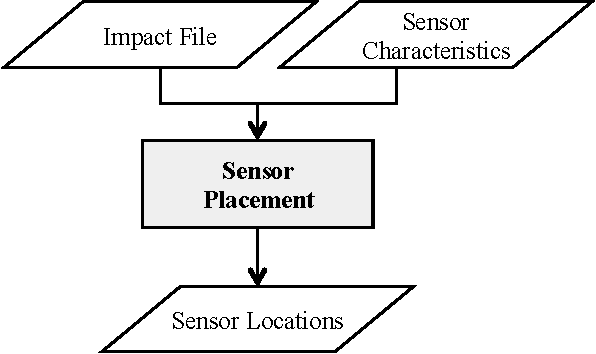
\includegraphics[scale=0.80]{graphics/sp_flowchart.pdf}
  \caption{Sensor placement flowchart.}
  \label{fig:sp-flowchart}
\end{figure}

The required input for the \code{sp} subcommand is an impact file and 
sensor characteristics. The impact file could be created by the \code{sim2Impact} subcommand,
or through some non-WST impact calculation process.
Multiple impact files can be used as input to the sensor placement problem. The other
required input is the sensor characteristics. These characteristics are supplied through
the \code{sp} WST configuration file as well as additional files that provide details 
on the cost and failure rates of the sensors.

Advanced features of the \code{sp} subcommand are discussed in
Section~\ref{chap:pmedian}. This includes a discussion of how to specify
feasible sensor locations and evaluation techniques. The section
also includes advanced sensor placement methods for computing a
bound on the quality of sensor networks, and techniques for minimizing
memory used during sensor placement: (a) aggregation of scenarios
and (b) skeletonization of the water distribution system network
model.



\section{Sensor Placement Formulations}\label{sp_formulation}

Several sensor placement optimization formulations are available
in the \code{sp} subcommand. The following formulations are described
below: expected-\/impact, robust optimization, side-constrained
and minimum cost formulations. WST also supports several sensor
placement formulations that are not documented yet: multi-stage
sensor placement and imperfect sensor models.

\subsection{Expected-\/Impact Formulation}\label{sp:average_formulation}

The most widely studied sensor placement formulation for a contamination warning system 
(CWS) design is to minimize the expected impact of an ensemble of contamination incidents 
given a fixed number of sensors. This formulation has also become the standard formulation 
in the \code{sp} subcommand, because it can be effectively used to select sensor placements 
in large water distribution networks.

A mixed-integer programming (MIP) formulation for expected-\/impact sensor placement is (eSP): 
\begin{align}
\textrm{minimize} \qquad & \sum_{a \in A} \alpha_a \sum_{i \in {\cal L}_a} d_{ai} x_{ai} \label{eqn:eSP} \\
\textrm{subject to} \qquad &\sum_{i\in {\cal L}_a} x_{ai} = 1 &&\forall a \in A\\ 
&x_{ai} \le s_i &&\forall a \in A, i \in {\cal L}_a\\  
&\sum_{i \in L} c_i s_i \le p\\ 
&s_i \in \{0,1\} &&\forall i \in L\\ 
&0 \leq x_{ai} \leq 1 &&\forall a \in A, i \in {\cal L}_a 
\end{align}

This MIP minimizes the expected impact of a set of contamination incidents defined by $A$. 
For each incident $a \in A$, $\alpha_a$ is the weight of incident $a$, which is typically a 
probability. This formulation integrates contamination impact calculations, which 
are reported at a set of locations from the full set, denoted $L$, 
where a location refers to a network node. For each incident $a$, ${\cal L}_a \subseteq L$ 
is the set of locations that can be contaminated by $a$. Thus, a sensor at a 
location $i \in {\cal L}_a$ can detect contamination from incident $a$ at the time 
contamination first arrives at location $i$. Each incident is witnessed 
by the first sensor to see it. For each incident $a \in A$ and location 
$i \in {\cal L}_a$, $d_{ai}$ defines the impact of the contamination incident $a$ 
if it is witnessed by location $i$. This impact metric assumes that as soon as a 
sensor witnesses contamination, then any further contamination impacts are mitigated 
(perhaps after a suitable delay that accounts for the response time of the water utility). 
The $s_i$ variables indicate where sensors are placed in the network, $c_i$ is 
the cost of placing a sensor at location $i$ and $p$ is the budget.

The $x_{ai}$ variables indicate whether incident $a$ is witnessed by a sensor at 
location $i$. They are defined as continuous variables between 0 and 1. 
In practice, there is always an optimal solution where $x_{ai}$ is binary. 
If $x_{ai}$ is fractional, then two or more equally good locations have sensors 
\citet{TEVASPOTCompendium10}. A given set of sensors might not be able to witness 
all contamination incidents. To account for this, $L$ contains a dummy location, $q$. 
The dummy location is assigned the impact if contamination was not detected at any node location. 
The dummy location is not a physical location in the network.
This dummy location is in all sets ${\cal L}_a$. If the dummy location witnesses
an incident, it generally means that no real sensor can detect that incident. The 
impact for this location is the impact of the contamination incident after the entire 
contaminant transport simulation has finished, which estimates the impact that 
would occur without an online sensor network. The impact of a dummy detection is greater
than all other impacts for each incident, so the witness variable $x_{ai}$ for the 
dummy will only be selected if no sensors have been placed that can detect this 
incident with smaller impact.

For examples on expected-\/impact sensor placement (eSP), see Example
\ref{sp_example1}, \ref{sp_example2} and \ref{sp_example3}.
\citet{BerHarPhiUbeWat06} describe eSP, and they note that this
formulation is identical to the well-\/known $p$-\/median facility
location problem \citep{MirFra90} when $c_i=1$. In the $p$-\/median
problem, $p$ facilities (e.g., central warehouses) are to be located
on $m$ potential sites such that the sum of distances $d_{ai}$
between each of $n$ customers (e.g., retail outlets) and the nearest
facility $i$ is minimized. In comparing eSP and $p$-\/median problems,
there is equivalence between (1) sensors and facilities, (2)
contamination incidents and customers and (3) contamination impacts
and distances. While eSP allows placement of at most $p$ sensors,
$p$-\/median formulations generally enforce placement of all $p$
facilities; in practice, the distinction is irrelevant unless $p$
approaches the number of possible locations. This equivalence enables the application of $p$-\/median 
solvers to eSP (see Example~\ref{sp_example3}).


\subsection{Robust Formulations}\label{sp:robust_formulation}

The eSP model described in Section \ref{sp:average_formulation} can
be viewed as optimizing one particular statistic of the distribution
of impacts defined by the contaminant transport simulations. However,
other statistics might provide more robust solutions that are 
less sensitive to changes in this distribution~\citep{WatHarMur06a, WatMurHar09}. 
Consider the following generalization of eSP:
\begin{align}
\textrm{minimize} \qquad &\textrm{Impact}_{f}(\alpha,d,x) \\
\textrm{subject to} \qquad &\sum_{i\in {\cal L}_a} x_{ai} = 1 &&\forall a \in A\\ 
&x_{ai} \le s_i &&\forall a \in A, i \in {\cal L}_a\\  
&\sum_{i \in L} c_i s_i \le p\\ 
&s_i \in \{0,1\} &&\forall i \in L\\ 
&0 \leq x_{ai} \leq 1 &&\forall a \in A, i \in {\cal L}_a 
\end{align}

The function $\textrm{Impact}_ {f}(\alpha,d,x)$ computes a statistic of the impact 
distribution. The following functions supported in WST have been developed by 
researchers to find robust solutions to optimization problems \citep{WatHarMur06a, WatMurHar09}:
\begin{itemize}
\item {\bfseries Mean:} This is the statistic used in eSP (Equation \ref{eqn:eSP})
\item {\bfseries VaR:} Value-\/at-\/Risk (VaR) is a percentile-\/based metric. 
Given a confidence level $\beta\in(0,1)$, the VaR is the value of the distribution 
at the $1-\beta$ percentile \citep{TopVlaZen02}. The value of VaR is less than 
the TCE value (see below).
Mathematically, suppose a random variable $W$ describes the distribution of possible 
impacts. The probability that $W$ is less than a value $w$ is denoted as $\P[W \le w]$. Then 
\begin{equation}
{\rm VaR}(W,\beta) = \min \{ w \mid \P[W \le w] \ge \beta \} 
\end{equation}
Note that the distribution $W$ changes with each sensor placement. Further, VaR 
can be computed using the $\alpha$, $d$ and $x$ values.
\item {\bfseries TCE:} The Tail-\/Conditioned Expectation (TCE) is a related 
metric that measures the conditional expectation of impact exceeding VaR at a 
given confidence level. Given a confidence level $1-\beta$, TCE is the expectation 
of the worst impacts whose likelihood sums to $\beta$. This value is between VaR and 
the worst-\/case value.
Mathematically, then
\begin{equation}
{\rm TCE}(\beta) = {\rm E}\left[ W \mid W \ge {\rm VaR}(\beta) \right]
\end{equation}
\item {\bfseries CVar:} The Conditional Value-\/at-\/Risk (CVaR) is a 
linearization of TCE investigated by \citet{rockafellar02cvar}. CVaR 
approximates TCE with a continuous, piecewise-\/linear function of $\beta$, 
which enables the use of CVaR in a MIP model.
\item {\bfseries Worst:} The worst impact value can be easily computed, since a 
finite number of contamination incidents are simulated. However, this statistic 
is sensitive to changes in the number of contamination incidents that are simulated; 
adding additional contamination incidents could significantly impact this statistic.
\end{itemize}

WST includes robust MIP reformulations of eSP for the the worst and CVar statistics. 
The reformulation to minimize the worst contamination impact is (wSP):
\begin{align}
\textrm{minimize} \qquad & w \label{eqn:wSP} \\
\textrm{subject to} \qquad & \alpha_a \sum_{i \in {\cal L}_a} d_{ai} x_{ai} \leq w && \forall a \in A\\
&\sum_{i\in {\cal L}_a} x_{ai} = 1 &&\forall a \in A\\ 
&x_{ai} \le s_i &&\forall a \in A, i \in {\cal L}_a\\  
&\sum_{i \in L} c_i s_i \le p\\ 
&s_i \in \{0,1\} &&\forall i \in L\\ 
&0 \leq x_{ai} \leq 1 &&\forall a \in A, i \in {\cal L}_a 
\end{align}
This is a standard formulation for the $p$-\/center problem \citep{Daskin95,ElloumiEtAl04}.

Similarly, the reformulation to minimize CVaR is (cvarSP):
\begin{align}
\textrm{minimize} \qquad & v + \frac{1}{\beta} \sum_{a \in A} \alpha_a y_a \label{eqn:cvarSP} \\
\textrm{subject to} \qquad & y_a \geq \sum_{i \in {\cal L}_a} d_{ai} x_{ai} - v && \forall a \in A\\
&y_q \geq 0 &&\forall a \in A \\
&\sum_{i\in {\cal L}_a} x_{ai} = 1 &&\forall a \in A\\ 
&x_{ai} \le s_i &&\forall a \in A, i \in {\cal L}_a\\  
&\sum_{i \in L} c_i s_i \le p\\ 
&s_i \in \{0,1\} &&\forall i \in L\\ 
&0 \leq x_{ai} \leq 1 &&\forall a \in A, i \in {\cal L}_a 
\end{align}
The variable $v$ represents $\rm VaR$, which is implicitly computed when this model is solved.
See \citet{rockafellar02cvar} for further discussion of CVaR formulations.

Note that these formulations share a core set of constraints and
variables with eSP. The difference in these models is how the
objective is expressed.
For examples on robust sensor placement (wSP and cvarSP), see Example \ref{sp_example4} and \ref{sp_example5}.


\subsection{Side-\/Constrained Formulation}\label{sp:sc_formulation}

Another natural generalization of eSP is to consider the addition
of side constraints that represent bounds on alternate objectives
or statistics. For example, consider a simple extension of eSP that
includes a single side-constraint (scSP):
\begin{align}
\textrm{minimize} \qquad & \sum_{a \in A} \alpha_a \sum_{i \in {\cal L}_a} d_{ai} x_{ai} \label{eqn:scSP} \\
\textrm{subject to} \qquad &\sum_{i\in {\cal L}_a} x_{ai} = 1 &&\forall a \in A\\ 
&x_{ai} \le s_i &&\forall a \in A, i \in {\cal L}_a\\  
&\sum_{i \in L} c_i s_i \le p\\ 
&s_i \in \{0,1\} &&\forall i \in L\\ 
&0 \leq x_{ai} \leq 1 &&\forall a \in A, i \in {\cal L}_a\\
& \sum_{a \in A} \alpha_a \sum_{i \in {\cal L}_a} \hat{d}_{ai} x_{ai} \leq G
\end{align}

The last constraint in this formulation bounds the value of an
impact statistic $\hat{d}_{ai}$. Note that this statistic could 
easily be used as the objective for (eSP). This can be
viewed as a goal constraint. Iteratively solving scSP for different
goals, $G$, provides an assessment of the trade-off between the impact
statistics in the objective and this constraint. Hence, the scSP formulation
provides a mechanism for analyzing trade-\/offs between different objectives.

WST provides general support for side-constraints beyond what is
represented in scSP, since multiple side-constraints can
be specified. Additionally, robust statistics can be specified.
For example, WST can express sensor placement formulations where
the mean impact is minimized while the worst-case impact is
constrained.
See Example \ref{sp_example6} for a demonstration of side-\/constrained sensor placement (scSP).


\subsection{Min-\/Cost Formulation}\label{sp:minCost_formulation}

The eSP model described in Section~\ref{sp:average_formulation}
minimizes expected contamination impact subject to a cost constraint
on the number of sensors that are installed. A related sensor
placement formulation is to minimize the cost of installing sensors
while constraining the contamination impact to be below a specified
threshold, $u$. 

For example, eSP can be reformulated to minimize cost (mcSP):
\begin{align}
\textrm{minimize} \qquad & \sum_{i \in L} c_i s_i \label{eqn:ceSP} \\
\textrm{subject to} \qquad &\sum_{i\in {\cal L}_a} x_{ai} = 1 &&\forall a \in A\\ 
&x_{ai} \le s_i &&\forall a \in A, i \in {\cal L}_a\\  
&\sum_{a \in A} \alpha_a \sum_{i \in {\cal L}_a} d_{ai} x_{ai} \leq u\\
&s_i \in \{0,1\} &&\forall i \in L\\ 
&0 \leq x_{ai} \leq 1 &&\forall a \in A, i \in {\cal L}_a 
\end{align}

See Example \ref{sp_example7} for a demonstration of min-\/cost sensor placement (mcSP).

\if 0
\subsection{Multiple Objective Formulation}\label{sp:multiObj_formulation}

CWS design generally requires the evaluation and optimization of a variety of 
performance objectives. Some performance objectives cannot be simultaneously optimized, 
and thus a CWS design must be selected from a trade-\/off between these   
objectives~\cite{WatGreHar04a}.

The \code{sp} subcommand supports the analysis of these trade-\/offs with the specification of additional 
constraints on impact measures. For example, a user can minimize the expected 
extent of contamination (EC) while constraining the worst-\/case time to 
detection (TD). The \code{sp} subcommand allows for the specification of more than one impact 
constraint. However, the sensor placement solvers cannot reliably optimize formulations with 
more than one impact constraint.

\subsection{Imperfect Sensors Formulation}\label{sp:imperfect_formulation}

The previous sensor placement formulations make the implicit assumption that 
sensors work perfectly. That is, they never fail to detect a contaminant when it 
exists, and they never generate an erroneous detection when no contaminant exists. 
In practice, sensors are imperfect, and they generate these types of errors.

The \code{sp} subcommand addresses this issue by supporting a formulation that models simple sensor 
failures~\cite{BerryCHLPW09}. Each sensor, $s_i$, has an associated probability
of failure, $p_i$. With these probabilities, the probability 
that a contamination incident will be detected by a particular sensor can be easily assessed. Thus, it 
is straightforward to compute the expected impact of a contamination incident.

This formulation does not explicitly allow for the specification of probabilities 
of false detections. These probabilities do not impact the performance of a CWS 
during a contamination incident. Instead, they impact the day-\/to-\/day maintenance
and use of the CWS; erroneous detections create work for the CWS users, which is an 
ongoing cost. The overall likelihood of false detections is simply a function of the
sensors that are selected. In cases where every sensor has the same likelihoods, this 
implies a simple constraint on the number of sensors. 
\fi

\section{Sensor Placement Solvers}

The \code{sp} subcommand performs optimization using a solver specified in the
configuration file. All of the solvers supported by the \code{sp} subcommand are practical
for small-\/sized water distribution networks, and heuristic
solvers can be used to find sensor placements for very large networks.

The \code{sp} subcommand interfaces with a variety of external
solvers that can be used to perform sensor placement. Several
different MIP solvers can be used to find a globally optimal solution
for the eSP MIP formulation. However, this might be a computationally
expensive process (especially for large problems), and the size of
the MIP formulation can become prohibitively large in some cases. 
A variety of public-domain and commercial solvers can be used by
the \code{sp} subcommand, including GLPK, CBC, PICO, CPLEX, GUROBI and
XPRESS.

% TODO - verify this text.  How do we name these solvers?

A greedy randomized adaptive sampling process (GRASP) heuristic 
performs sensor placement optimization without
explicitly creating a MIP formulation. Thus, this solver uses much
less memory, and it usually runs very quickly. Although the GRASP
heuristic does not guarantee that a globally optimal solution is
found, it has proven effective at finding optimal solutions to a
variety of large-scale applications. Two different implementations
of the GRASP solvers can be used: an AT\&T commercial solver (att\_grasp)
or an open-source implementation of this solver (snl\_grasp).

% TODO - verify this text.  What is the status of this solver?

The Lagrangian heuristic uses the structure of the $p$-\/median MIP
formulation (eSP) to find near-optimal solutions while computing a
lower bound on the best possible solution.


\section{\code{sp} Subcommand}

The \code{sp} subcommand is executed with the following command:

\begin{unknownListing}
wst sp <configfile>
\end{unknownListing}

where \code{configfile} is a WST configuration file in the YAML format. 

The \code{---help} option prints information about this subcommand, such as usage,
arguments and a brief description:

\begin{unknownListing}
wst sp --help
\end{unknownListing}

Two other options can be used to print help information. 
The \code{---help-problems} option prints a table of the different types of 
optimization problems that can be solved with the \code{sp} subcommand. For example, 
the following is a description of the standard problem solved by the \code{sp} subcommand (eSP):

\begin{unknownListing}
default, p-median, average-case perfect-sensor
---------------------------------------------- 
mean obj
0 constraints
perfect
single obj
1 stage
exact
\end{unknownListing}

The first row lists the different names that can be used to specify
this problem type. These are synonyms, since the standard problem,
eSP, is a $p$-\/median problem where the objective is an average statistic.
This is also the standard perfect-sensor formulation, where all
sensors are assumed to work perfectly without failures.
The six rows following the dashed lines are different characteristics of this problem: 
\begin{enumerate}
\item the type of objective used
\item the number of side-constraints
\item specify whether sensors are perfect (i.e., without failures) or whether they can fail
\item the number of objectives
\item the number of stages (i.e., time steps) in the sensor placement formulation
\item the type of solution that is required (e.g., an exact solution versus any feasible solution).
\end{enumerate}
These six characteristics are used by the \code{sp} subcommand 
to verify the suitability of solvers that are specified for optimization.

The \code{---help-solvers} option prints a table of the different solvers that can
be applied to perform optimization. For example, the following is a description
of the solvers that can be used to optimize \code{average-case perfect-sensor} problems (which is the default):

\begin{unknownListing}
Problem Type                  Solver        Modeling Language  
======================================================================
average-case perfect-sensor   *att_grasp     none               
average-case perfect-sensor   *cbc           pyomo              
average-case perfect-sensor   *cplex         pyomo              
average-case perfect-sensor   *glpk          pyomo              
average-case perfect-sensor    gurobi        pyomo              
average-case perfect-sensor   *lagrangian    none               
average-case perfect-sensor    pico          ampl               
average-case perfect-sensor    pico          pyomo              
average-case perfect-sensor   *snl_grasp     none               
average-case perfect-sensor    xpress        pyomo     
\end{unknownListing}

Solvers highlighted with an asterisk are available in the current
installation of WST. The modeling language indicates whether AMPL
\citep{AMPL}, Pyomo \citep{PYOMO} or neither is used to solve sensor
placement optimization problem. Note that GLPK includes a modeling
tool that includes a subset of AMPL. Thus, problems that require
AMPL can be solved if either AMPL or GLPK is installed.


\subsection{Configuration File}

The \code{sp} subcommand generates a template configuration file using the following command line:
\begin{unknownListing}
wst sp --template <configfile>
\end{unknownListing}

The template configuration file for the \code{sp} subcommand is shown in Figure \ref{fig:sp_template}.  
Brief descriptions of the options are included in the template after the \# character.  

\begin{figure}[h!]
	\unknownInputListing{examples/sp_config.yml}{}{1}{24}
	\caption[The \code{sp} configuration template file]{The \code{sp} configuration template file (\textit{continued in Figure \ref{fig:sp_template_ctd}}).}
	\label{fig:sp_template}
\end{figure}

\begin{figure}[h!]
	\unknownInputListing{examples/sp_config.yml}{}{25}{67}
	\caption[The \code{sp} configuration template file (ctd.)]{The \code{sp} configuration template file (\textit{continued from Figure \ref{fig:sp_template}}).}
	\label{fig:sp_template_ctd}
\end{figure}

\clearpage
\subsection{Configuration Options}

Full descriptions of the WST configuration options used by the \code{sp} subcommand are listed below.
\begin{description}[topsep=0pt,parsep=0.5em,itemsep=-0.4em]
  \item[{impact data}]\hfill
  \begin{description}[topsep=0pt,parsep=0.5em,itemsep=-0.4em]
    \item[{name}]\hfill
\\The name of the impact block that is used in the objective or constraint block.
                
                Required input.
                
    \item[{impact file}]\hfill
\\The name of the impact file that is created by \code{sim2Impact} and 
                contains the detection time and the total
                impact given a sensor at that node is the first to detect
                contamination from that scenario. 
                The impact file format is documented in File Formats Section \ref{formats_impactFile}.
                
                Required input.
                
    \item[{nodemap file}]\hfill
\\The name of the nodemap file that is created by \code{sim2Impact} and 
                maps sensor placement ids to the network node labels. 
                The nodemap file format is documented in File Formats Section \ref{formats_nodeFile}.
                
                Required input.
                
    \item[{weight file}]\hfill
\\The name of the weight file that specifies the weights for contamination
                incidents. This file supports the optimization of weighted
                impact metrics. 
                The weight file format is documented in File Formats Section \ref{formats_weightFile}.
                
                Optional input; by default, incidents are optimized with weight 1.
  \end{description}

  \item[{cost}]\hfill
  \begin{description}[topsep=0pt,parsep=0.5em,itemsep=-0.4em]
    \item[{name}]\hfill
\\The name of the cost block that is used in the objective or constraint block.
                
                Optional input.
    \item[{cost file}]\hfill
\\The name of the cost file that contains the costs for the installation of
                sensors throughout the distribution network. This file contains
                EPANET ID/cost pairs.
                The cost file format is documented in File Formats Section \ref{formats_costFile}.
                
                Optional input.
  \end{description}
  \item[{objective}]\hfill
  \begin{description}[topsep=0pt,parsep=0.5em,itemsep=-0.4em]
    \item[{name}]\hfill
\\The name of the objective block that is used in sensor placement block.
                
                Required input.
    \item[{goal}]\hfill
\\The objective of the optimization process that defines what is going to minimized. 
                The options are the name of the impact block, the name of the cost block, 
                the number of sensors (NS) or the number of failed detections (NFD).
				
				Required input.
    \item[{statistic}]\hfill
      \\The objective statistic. The TOTAL
      statistic is used when the goal is NS                             or
      NFD. When the goal is to compute a                             statistic
      of an impact block, the options                             are MEAN,
      MEDIAN, VAR, TCE, CVAR, TOTAL                             or WORST. For
      example, MEAN will minimize                             the mean impacts
      over all of the                             contamination scenarios,
      while WORST                             will only minimize the worst
      impacts                             from the ensemble of contamination
      scenarios.                                  Required input.
    \item[{gamma}]\hfill
      \\The value of gamma that specifies the                 fraction of the
      distribution of impacts that will                 be used to compute the
      VAR, CVAR and TCE statistics.                 Gamma is assumed to be in
      the interval (0,1], which means                  that gamma can be
      greater than zero but less than or equal to one. It                 can
      be interpreted as specifying the 100*gamma                 percent of
      the worst contamination incidents that                 are used for
      these calculations.                  Required input for VAR or CVAR
      objective statistics,                 default = 0.05.
  \end{description}
  \item[{constraint}]\hfill
  \begin{description}[topsep=0pt,parsep=0.5em,itemsep=-0.4em]
    \item[{name}]\hfill
\\The name of the constraint block that is used in sensor placement block.
                
                Required input.
    \item[{goal}]\hfill
\\The constraint goal. The options are the name of the impact block name, 
                the name of the cost block, the number of sensors (NS) or the number of failed detections (NFD).
                
                Required input.
    \item[{statistic}]\hfill
\\The constraint statistic. The TOTAL
                statistic is used when the goal is NS
                or NFD. When the goal is to compute a
                statistic of an impact block, the options
                are MEAN, MEDIAN, VAR, TCE, CVAR, TOTAL
                or WORST. For example, MEAN will constrain
                the mean impacts over all of the
                contamination scenarios, while WORST
                will only constrain the worst impacts
                from the ensemble of contamination
                scenarios.

                Required input.
    \item[{gamma}]\hfill
\\The value of gamma that specifies the fraction of the distribution of impacts that
                will be used to compute the VAR, CVAR and TCE statistics. Gamma
                is assumed to be in the interval (0,1], which means that gamma 
				can be greater than zero but less than or equal to one. It can be interpreted
                as specifying the 100*gamma percent of the worst contamination
                incidents that are used for these calculations.  
                
                Required input for VAR or CVAR objective statistics, default = 0.05.
    \item[{bound}]\hfill
\\The upper bound on the constraint.
                
                Optional input.
  \end{description}
  \item[{aggregate}]\hfill
  \begin{description}[topsep=0pt,parsep=0.5em,itemsep=-0.4em]
    \item[{name}]\hfill
\\The name of the aggregation block that is used in sensor placement block.
                
                Optional input.
    \item[{type}]\hfill
\\The type of aggregation used to reduce the size of the sensor placement problem.  
                The options are THRESHOLD, PERCENT or RATIO.

                THRESHOLD is used to aggregate similar impacts by specifying a goal and a value.  
                This is used to reduce the total size of the sensor placement formulation (for large problems).
                Solutions generated with non-zero thresholds are not guaranteed
                to be globally optimal.

                PERCENT is an alternative method to compute the aggregation threshold 
                in which the value (of the goal-value pair) is a real number between 0.0 and 1.0. 
                Over all contamination incidents, compute the maximum difference, d, between the impact of the
                contamination incident if it is not detected and the impact if it is detected
                at the earliest possible feasible location and set the aggregation threshold to 
                d times the aggregation percent. If both THRESHOLD and PERCENT are set to valid values, 
                then PERCENT takes priority.

                RATIO is also specified with a goal-value pair in which value is a real number between
                0.0 and 1.0.
                
                Optional input.
    \item[{goal}]\hfill
\\The aggregation goal for the aggregation type.
                
                Optional input.
    \item[{value}]\hfill
\\The aggregation value for the aggregation type. If the aggregation type is PERCENT or RATIO,
                then this value is a real number between 0.0 and 1.0.
                
                Optional input.
    \item[{conserve memory}]\hfill
\\The maximum number of impact files that should be read into memory 
                at any one time. This option allows impact files to be processed in 
                a memory conserving mode if location aggregation is chosen and the original impact
                files are very large. For example, a conserve memory value of 10000 requests
                that no more than 10000 impacts should be read into memory at any one 
                time while the original impact files are being processed into smaller
                aggregated files.  
				
				Optional input, default = zero to turn off this option.
    \item[{distinguish detection}]\hfill
\\A goal for which aggregation should not allow incidents to
                become trivial. If the aggregation threshold is so large that all
                locations, including the dummy, would form a single superlocation,
                this forces the dummy to be in a superlocation by itself. Thus,
                the sensor placement will distinguish between detecting and not
                detecting. This option can be listed multiple times, to specify
                multiple goals. 
                
                Optional input, default = 0.
    \item[{disable aggregation}]\hfill
\\Disable aggregation for this goal, even at value zero, which
                would incur no error. Each witness incident will be in a separate
                superlocation. This option can be listed multiple times to
                specify multiple goals. ALL can be used to specify
                all goals. 
                
                Optional input, default = 0.
  \end{description}
  \item[{imperfect}]\hfill
  \begin{description}[topsep=0pt,parsep=0.5em,itemsep=-0.4em]
    \item[{name}]\hfill
\\The name of the imperfect block that is used in sensor placement block.
                
                Optional input.
    \item[{sensor class file}]\hfill
\\The name of the imperfect sensor class file that defines the detection probabilities
                for all sensor categories. It is used with the imperfect-sensor model 
                and must be specified in conjunction with a imperfect junction class file.
                The imperfect sensor class file format is documented in File Formats Section \ref{formats_sensorClass}.
                
                Optional input.
    \item[{junction class file}]\hfill
\\The name of the imperfect junction class file that defines a sensor category for
                each network node. It is used with the imperfect-sensor model and
                must be specified in conjunction with a imperfect sensor class file.
                The imperfect junction class file format is documented in File Formats Section \ref{formats_junctionClass}.
                
                Optional input.
  \end{description}
  \item[{sensor placement}]\hfill
  \begin{description}[topsep=0pt,parsep=0.5em,itemsep=-0.4em]
    \item[{type}]\hfill
\\The sensor placement problem type. The command \code{wst sp ---help-problems} 
                provides a list of problem types for sensor placement. For example, average-case perfect-sensor
                is the standard problem type for sensor placement, since it uses the mean statistic, 
                zero constraints, single objective and perfect sensors. 
                
                Required option, default = average-case perfect-sensor.
    \item[{modeling language}]\hfill
\\The modeling language to generate the sensor placement optimization 
                problem. The options are NONE, PYOMO or AMPL. 

                Required input, default = NONE.
    \item[{objective}]\hfill
\\The name of the objective block previously defined to be used in sensor placement.
                
                Required input.
    \item[{constraint}]\hfill
\\The name of the constraint block previously defined to be used in sensor placement.
                
                Required input.
    \item[{imperfect}]\hfill
\\The name of the imperfect block previously defined to be used in sensor placement.
                
                Optional input.
    \item[{aggregate}]\hfill
\\The name of the aggregate block previously defined to be used in sensor placement.
                
                Optional input.
    \item[{compute bound}]\hfill
\\A flag to indicate if bounds should be computed on the sensor placement
                solution. The options are true or false. 
                
                Optional input, default = false.
    \item[{presolve}]\hfill
\\A flag to indicate if the sensor placement problem should be presolved. 
                The options are true or false. 
                
                Optional input, default = true.
    \item[{compute greedy ranking}]\hfill
\\A flag to indicate if a greedy ranking of the sensor locations should be calculated. 
                The options are true or false. 
                
                Optional input, default = false.
    \item[{location}]\hfill
    \begin{description}[topsep=0pt,parsep=0.5em,itemsep=-0.4em]
      \item[{feasible nodes}]\hfill
\\A list that defines nodes that can be considered for the sensor placement problem.
                The options are:
                (1) ALL, which specifies all nodes as feasible sensor locations;
                (2) NZD, which specifies all non-zero demand nodes as feasible sensor locations;
                (3) a list of EPANET node IDs, which identifies specific nodes as feasible sensor locations; 
                (4) a filename, which references a space or comma separated file containing a list of 
                specific nodes as feasible sensor locations; or
                (5) NONE, which indicates this option is ignored.
                
                Required input, default = ALL.
      \item[{infeasible nodes}]\hfill
\\A list that defines nodes that cannot be considered for the sensor placement problem.
                The options are:
                (1) ALL, which specifies all nodes as infeasible sensor locations;
                (2) NZD, which specifies non-zero demand nodes as infeasible sensor locations;
                (3) a list of EPANET node IDs, which identifies specific nodes as infeasible sensor locations;
                (4) a filename, which references a space or comma separated file containing a list of 
                specific nodes as infeasible sensor locations; or
                (5) NONE, which indicates this option is ignored.
                
                Optional input, default = NONE.
      \item[{fixed nodes}]\hfill
\\A list that defines nodes that are already sensor locations.
                The options are:
                (1) ALL, which specifies all nodes as fixed sensor locations;
                (2) NZD, which specifies non-zero demand nodes as fixed sensor locations;
                (3) a list of EPANET node IDs, which identifies specific nodes as fixed sensor locations; 
                (4) a filename, which references a space or comma separated file containing a list of 
                specific nodes as fixed sensor locations; or
                (5) NONE, which indicates this option is ignored.
                
                Optional input, default = NONE.
      \item[{unfixed nodes}]\hfill
\\A list that defines nodes that are unfixed sensor locations.
                The options are:
                (1) ALL, which specifies all nodes as unfixed sensor locations;
                (2) NZD, which specifies non-zero demand nodes as unfixed sensor locations;
                (3) a list of EPANET node IDs, which identifies specific nodes as unfixed sensor locations; 
                (4) a filename, which references a space or comma separated file containing a list of 
                specific nodes as unfixed sensor locations; or
                (5) NONE, which indicates this option is ignored.
                
                Optional input, default = NONE.
    \end{description}
  \end{description}
  \item[{solver}]\hfill
  \begin{description}[topsep=0pt,parsep=0.5em,itemsep=-0.4em]
    \item[{type}]\hfill
\\The solver type. Each component of WST
				(e.g., sensor placement, flushing response, booster 
				placement) has different 
				solvers available. More specific details are provided in 
				the subcommand's chapter.
                
                Required input.
    \item[{options}]\hfill
\\A list of options associated with a specific solver type. More
            information on the options available for a specific solver
            is provided in the solver's documentation. The Getting
            Started Section \ref{dependencies} provides links to the
            different solvers.
            
            Optional input.
    \item[{threads}]\hfill
\\The maximum number of threads or function evaluations the solver is
                allowed to use.  This option is not available to all solvers or all analyses.
                
                Optional input.
    \item[{logfile}]\hfill
\\The name of a file to output the results of the solver.
                
                Optional input.
    \item[{verbose}]\hfill
\\The solver verbosity level.
                
                Optional input, default = 0 (lowest level).
    \item[{initial points}]\hfill
    \begin{description}[topsep=0pt,parsep=0.5em,itemsep=-0.4em]
      \item[{nodes}]\hfill
\\A list of node locations (EPANET IDs) to begin the optimization
        process. Currently, this option is only supported for the
        network solver used in the flushing and booster\_msx
        subcommands. This input causes an error for other subcommands.
        
        Optional input.
      \item[{pipes}]\hfill
\\A list of pipe locations (EPANET IDs) to begin the optimization
        process. Currently, this option is only supported for the
        network solver used in the flushing subcommand. This input causes an error for other subcommands.
        
        Optional input.
    \end{description}
  \end{description}
  \item[{configure}]\hfill
  \begin{description}[topsep=0pt,parsep=0.5em,itemsep=-0.4em]
    \item[{output prefix}]\hfill
\\The prefix used for all output files.
                
                Required input.
    \item[{output directory}]\hfill
      \\The output directory to store the results.
    \item[{debug}]\hfill
\\The debugging level (0 or 1) that indicates the amount of debugging 
                information printed to the screen, log file and output yml file. 
                
                Optional input, default = 0 (lowest level).
  \end{description}
\end{description}


\subsection{Subcommand Output}

The \code{sp} subcommand creates several output files.
The YAML file called <output prefix>sp\_output.yml contains the sensor locations,
final impact metric, the run date and CPU time. For some solvers, the
lower and upper bound on the objective is reported.   
The log file called <output prefix>sp\_output.log contains basic debugging information. 
A visualization YAML configuration file called
<output prefix>sp\_output\_vis.yml is also created and can be used to generate 
network graphics of the sensor placement solution using the \code{visualization} 
subcommand. The correct EPANET INP file must be included in the visualization YAML configuration 
file for the graphic to display properly.

The \code{sp} subcommand also outputs information a file named <output prefix>\_evalsensor.out 
That file includes the following data:
\begin{itemize}
\item {\bfseries Objective:} The impact metric value achieved with the sensor network design.
\item {\bfseries Lower bound:} The lower bound on the impact metric with the sensor network design.
\item {\bfseries Upper bound:} The upper bound on the impact metric with the sensor network design.
\item {\bfseries Solutions:} The internal node indices used by \code{sp} for the sensor network design.
\item {\bfseries Locations:} The EPANET junction labels for the sensor placement locations.
\item {\bfseries Sensor placement ID:} An integer ID used to distinguish the sensor network design.
\item {\bfseries Number of sensors:} The number of sensors in the sensor network design.
\item {\bfseries Total cost:} The cost of the sensor network design, which could be non-zero if cost data is provided.
\item {\bfseries Sensor node IDs:} The internal node indices used by \code{sp} for the sensor network design. The same as Solutions.
\item {\bfseries Sensor junctions:} The EPANET junction labels for the sensor placement locations. The same as Locations.
\item {\bfseries Impact file:} The name of the impact file used in the sensor network design.
\item {\bfseries Number of events:} The number of contamination scenarios that were simulated.
\end{itemize}

The performance of the sensor network design is summarized for each impact data file 
specified in the configuration file. The impact statistics included are: 
\begin{itemize}
\item {\bfseries Min impact:} The minimum impact over all contamination
incidents simulated. Assuming that a sensor protects the node
at which it is placed, this statistic will typically be zero.
\item {\bfseries Mean impact:} The mean (or average) impact over all
contamination incidents simulated.
\item {\bfseries Lower quartile impact:} 25\% of the contamination incidents,
weighted by their likelihood, have an impact value less than this quartile.
\item {\bfseries Median impact:} 50\% of the contamination incidents simulated, weighted
by their likelihood, have an impact value less than this quartile.
\item {\bfseries Upper quartile impact:} 75\% of the contamination incidents simulated,
weighted by their likelihood, have an impact value less than this quartile.
\item {\bfseries Value at Risk (VaR):} VaR is the minimum value
for which $100\times(1-\beta)$\% of the contamination incidents simulated have a smaller
impact, in which $\beta$ is a user-defined percentage between $ 0.0 < \beta < 1.0$.
\item {\bfseries TCE:} The tailed-\/conditioned expectation (TCE)
is the mean value of the impacts that are greater than or equal to VaR.
\item {\bfseries Worst impact:} The worst impact over all contamination
incidents simulated.
\end{itemize}

If the \code{[compute greedy ranking]} option is used, a greedy sensor placement is printed 
to <output prefix>\_evalsensor.out. The greedy ranking places sensors one-\/at-\/a-\/time at the locations 
in the optimal sensor network design by consecutively minimizing the mean impact 
of placing each sensor. This analysis gives a sense of the relative priorities for these
sensors. The greedy ranking is listed in terms of the sensor node IDs used by the 
\code{sp} subcommand. The corresponding EPANET node ID is listed at the top of the file.

\section{Sensor Placement Examples}\label{sp_example}

The following examples illustrate common ways that the \code{sp} subcommand can be used. 
Additional examples using the \code{sp} subcommand are provided in Section~\ref{chap:pmedian}.

\subsection{Example 1: Solving eSP with a MIP Solver}
\label{sp_example1}

The first example uses the configuration file, sp\_ex1.yml, shown in Figure \ref{fig:sp_ex1}.
It specifies the impact file as {\outputprefix}\_ec.impact created by the \code{sim2Impact} subcommand 
using the extent of contamination (EC) impact metric and EPANET Example Network 3. 
The objective is to minimize the mean EC over all contamination incidents 
simulated while limiting the number of sensors (NS) to no more than five. 
The solver is the GLPK mixed-integer programming (MIP) solver, 
which finds globally optimal sensor placements. In addition, the greedy ranking 
option is used.

\begin{figure}[h]
  \unknownInputListing{../../examples/sp_ex1.yml}{}{1}{27}
  \caption{The \code{sp} configuration file for example 1.}
  \label{fig:sp_ex1}
\end{figure}

The \code{sp} subcommand is executed using the following command line:

\begin{unknownListing}
wst sp sp_ex1.yml
\end{unknownListing}

The \code{sp} subcommand for example 1 generates the YAML output file, {\outputprefix}sp\_output.yml, 
which summarizes the sensor placement results (see Figure \ref{fig:sp_ex1_yml}). 
The sensor network design places sensors at nodes 113, 121, 141, 163 and 209 to achieve 
an objective value of approximately 8655 of pipe feet contaminated.  

\begin{figure}[h]
  \unknownInputListing{examples/sp/sp_ex1_output.yml}{}{1}{14}
  \caption{The \code{sp} YAML output file for example 1.}
  \label{fig:sp_ex1_yml}
\end{figure}

The {\outputprefix}\_evalsensor.out file for the first \code{sp} subcommand example is 
shown in Figure \ref{fig:sp_ex1_evalsensor}. It displays the 
same sensor network design and impact value as in the YAML output file. 
It also includes the greedy ranking of the sensor network design, in which
a sensor at node 163 would provide the greatest reduction in the impact 
followed by sensors at nodes 209, 113, 141 and 121. The first value in the 
greedy ranking is -1 (or the dummy location value), which gives the impact if no 
sensors are placed in the network.

\begin{figure}[h]
  \unknownInputListing{examples/sp/sp_ex1_evalsensor.out}{}{1}{27}
  \caption{The evalsensor output for \code{sp} example 1.}
  \label{fig:sp_ex1_evalsensor}
\end{figure}

\FloatBarrier 
\subsection{Example 2: Evaluating Solutions to eSP with Multiple Impact Files}
\label{sp_example2}

The \code{sp} subcommand can also be configured to evaluate a sensor network design using
impact data not used for optimization. The second example uses the configuration 
file, sp\_ex2.yml, shown in Figure \ref{fig:sp_ex2}. Several impact files, 
{\outputprefix}\_ec.impact and {\outputprefix}\_mc.impact, are defined in the 
impact block of the WST configuration file. The objective of the sensor placement 
optimization is to minimize the mean EC impact metric. The optimal sensor 
network design is then evaluated against the mass consumed (MC) impact metric.

\begin{figure}[h]
  \unknownInputListing{../../examples/sp_ex2.yml}{}{1}{30}
  \caption{The \code{sp} configuration file for example 2.}
  \label{fig:sp_ex2}
\end{figure}

The \code{sp} subcommand is executed using the following command line:

\begin{unknownListing}
wst sp sp_ex2.yml
\end{unknownListing}

All of the impact files specified in the configuration file are
used when evaluating the sensor placement, and a greedy sensor
placement is generated for each (see Figure \ref{fig:sp_ex2_evalsensor}).
The sensor network design optimized for EC has a mean MC
impact of 56320 mg, while the EC impact is 8655 feet. 
The greedy ranking of the sensors is different for
the two different impact metrics. A sensor at node 209 would be the
first sensor placed for the MC impact metric compared to a sensor
at node 163 for the EC impact metric. The greedy ranking is a cumulative 
effect of adding more sensors, so the -1 value is the impact of having no 
sensors in the network and the next sensor location is the impact of adding 
one sensor and so forth down the list.

\begin{figure}[h]
  \unknownInputListing{examples/sp/sp_ex2_evalsensor.out}{}{1}{47}
  \caption{The evalsensor output for \code{sp} example 2.}
  \label{fig:sp_ex2_evalsensor}
\end{figure}

\FloatBarrier 
\subsection{Example 3: Solving eSP with a GRASP Solver}
\label{sp_example3}

The third example illustrates the use of a heuristic solver for sensor placement. 
A GRASP heuristic iteratively applies local search to adaptively sample locations. 
Two GRASP heuristics are provided in WST. The AT\&T GRASP solver is based on the
AT\&T \code{popstar} software, and it can be used for research
purposes. The SNL GRASP solver is a new implementation of
the GRASP algorithm in popstar. Example 3 uses the configuration file, sp\_ex3.yml, which is 
shown in Figure \ref{fig:sp_ex3}. The sensor placement parameters are the same as 
in Example~\ref{sp_example1}; the only difference is that the SNL GRASP solver is used instead of GLPK.

\begin{figure}[h]
  \unknownInputListing{../../examples/sp_ex3.yml}{}{1}{27}
  \caption{The \code{sp} configuration file for example 3.}
  \label{fig:sp_ex3}
\end{figure}

The \code{sp} subcommand is executed using the following command line:

\begin{unknownListing}
wst sp sp_ex3.yml
\end{unknownListing}

The {\outputprefix}\_evalsensor.out file for example 3 is shown in Figure~\ref{fig:sp_ex3_evalsensor}. 
The SNL GRASP heuristic solver finds the same solution found by 
the GLPK solver in example 1. In addition, the solver found 
another solution during the search with the same performance. Since GRASP is a heuristic solver, 
it is not guaranteed to find sensor placements with the globally optimal value. 
However, GRASP has proven capable of finding optimal or near-optimal solutions
even for large sensor placement problems. While the MIP solver in example 1
provided an upper and lower bound on the value of the solution, the GRASP solver
does not generate these bounds since it is a heuristic. 

GRASP is a heuristic search that is partly dependent on a random
number generator. Consequently, users should not expect the solver
to give identical results when run on different machines or operating
systems. Thus, the solution shown in Figure \ref{fig:sp_ex3_evalsensor}
might not be the solution on everyone's machine.

\begin{figure}[h]
  \unknownInputListing{examples/sp/sp_ex3_evalsensor.out}{}{1}{27}
  \caption{The evalsensor output for \code{sp} example 3.}
  \label{fig:sp_ex3_evalsensor}
\end{figure}


\FloatBarrier 
\subsection{Example 4: Solving wSP with a MIP Solver}
\label{sp_example4}
The subsequent examples illustrate the use of WST to solve more
complex sensor placement problems. In most cases, these problems are
significantly harder to solve than eSP. MIP solvers are used in the following 
examples to ensure consistency in the solution, but the time required to solve 
these problems is non-trivial.

The fourth example uses the configuration file, sp\_ex4.yml, shown
in Figure \ref{fig:sp_ex4}. The objective is to minimize the
worst-case expected contamination over all contamination incidents
simulated while limiting the number of sensors to no more than
five. The solver is the CBC solver, which finds globally optimal 
sensor placements. In addition, the greedy ranking option is used.

\begin{figure}[h]
  \unknownInputListing{../../examples/sp_ex4.yml}{}{1}{27}
  \caption{The \code{sp} configuration file for example 4.}
  \label{fig:sp_ex4}
\end{figure}

The \code{sp} subcommand is executed using the following command line:

\begin{unknownListing}
wst sp sp_ex4.yml
\end{unknownListing}

The {\outputprefix}\_evalsensor.out file for this example is shown in Figure
\ref{fig:sp_ex4_evalsensor}. Compared with the results from example 1, this
solution has a lower maximum impact for EC and a higher mean impact
for EC. This reflects the difference in the objectives of these two
problems.

\begin{figure}[h]
  \unknownInputListing{examples/sp/sp_ex4_evalsensor.out}{}{1}{27}
  \caption{The evalsensor output for \code{sp} example 4.}
  \label{fig:sp_ex4_evalsensor}
\end{figure}



\FloatBarrier 
\subsection{Example 5: Solving cvarSP with a MIP Solver}
\label{sp_example5}

Example 5 uses the configuration file, sp\_ex5.yml, shown in Figure
\ref{fig:sp_ex5}. The objective is to minimize the conditional
value-at-risk (CVaR) over all contamination incidents simulated
while limiting the number of sensors to no more than five. The
parameter $\gamma = 0.05$ specifies the weight of the tail that is
used to measure CVaR (CVaR approximates the mean impact of the
$5\%$ worst scenarios). Hence, minimizing CVaR is similar to
minimizing the worst-case; the difference is that minimizing CVaR
reduces the impact of all of the worst $5\%$ of the scenarios. 
The GLPK solver and the greedy ranking option are used.

\begin{figure}[h]
  \unknownInputListing{../../examples/sp_ex5.yml}{}{1}{28}
  \caption{The \code{sp} configuration file for example 5.}
  \label{fig:sp_ex5}
\end{figure}

The \code{sp} subcommand is executed using the following command line:

\begin{unknownListing}
wst sp sp_ex5.yml
\end{unknownListing}

The {\outputprefix}\_evalsensor.out file for this example is shown in Figure
\ref{fig:sp_ex5_evalsensor}. Compared with the results of example 1, this
solution has a lower TCE for EC and a higher mean impact for EC.
Compared with the results of example 4, this solution has the same maximum
impact for EC and a lower TCE impact for EC. Both of these comparisons
reflect the difference in the objectives of these problems.

\begin{figure}[h]
  \unknownInputListing{examples/sp/sp_ex5_evalsensor.out}{}{1}{27}
  \caption{The evalsensor output for \code{sp} example 5.}
  \label{fig:sp_ex5_evalsensor}
\end{figure}



\FloatBarrier 
\subsection{Example 6: Solving scSP with a MIP Solver}
\label{sp_example6}

This example considers two sensor placement problems where a side constraint
is used to limit the feasible sensor networks.
Example 6a uses the configuration file, sp\_ex6a.yml, shown in Figure
\ref{fig:sp_ex6a}. The objective is to minimize the mean contamination 
impact for EC over all contamination incidents simulated
while limiting (1) the number of sensors to no more than five and (2) the
mean contamination impact for MC to no more than 50000.0.
The GLPK solver and the greedy ranking option are used.

\begin{figure}[h]
  \unknownInputListing{../../examples/sp_ex6a.yml}{}{1}{36}
  \caption{The \code{sp} configuration file for example 6a.}
  \label{fig:sp_ex6a}
\end{figure}

The \code{sp} subcommand is executed using the following command line:

\begin{unknownListing}
wst sp sp_ex6a.yml
\end{unknownListing}

The {\outputprefix}\_evalsensor.out file for this example is shown in Figure
\ref{fig:sp_ex6a_evalsensor}. By comparison with example 1, this
solution has a higher mean impact for EC and a lower mean impact for MC.
This comparison reflects how adding constraints to the formulation in
example 1 leads to a worse solution for the objective while satisfying a
side constraint.

\begin{figure}[h]
  \unknownInputListing{examples/sp/sp_ex6a_evalsensor.out}{}{1}{47}
  \caption{The evalsensor output for \code{sp} example 6a.}
  \label{fig:sp_ex6a_evalsensor}
\end{figure}

Example 6b illustrates that a different impact statistic can be
used in a side-constraint than is used in the objective.  Note that
the solution in Figure~\ref{fig:sp_ex6a_evalsensor} has a worst-case
impact statistic of $143999.0$ The configuration file in
Figure~\ref{fig:sp_ex6a} uses a side-constraint where the MC impacts
are constrained by the worst-case value of $150000.0$.

\begin{figure}[h]
  \unknownInputListing{../../examples/sp_ex6b.yml}{}{1}{36}
  \caption{The \code{sp} configuration file for example 6b.}
  \label{fig:sp_ex6a}
\end{figure}

Figure~\ref{fig:sp_ex6b_evalsensor} shows the solution to Example
6b.  This solution is similar to the solution in Example 6a.  Although
the solution has the same worst-case value for MC impacts, the mean
MC impacts are larger.

\begin{figure}[h]
  \unknownInputListing{examples/sp/sp_ex6b_evalsensor.out}{}{1}{47}
  \caption{The evalsensor output for \code{sp} example 6b.}
  \label{fig:sp_ex6b_evalsensor}
\end{figure}


\FloatBarrier 
\subsection{Example 7: Solving mcSP with a MIP Solver}
\label{sp_example7}

Example 7 uses the configuration file, sp\_ex7.yml, shown in Figure
\ref{fig:sp_ex7}. The objective is to minimize the number of sensors
while limiting the mean contamination impact for EC over all
contamination incidents to no more than 5000.0. The 
CBC solver and the greedy ranking option are used.

\begin{figure}[h]
  \unknownInputListing{../../examples/sp_ex7.yml}{}{1}{27}
  \caption{The \code{sp} configuration file for example 7.}
  \label{fig:sp_ex7}
\end{figure}

The \code{sp} subcommand is executed using the following command line:

\begin{unknownListing}
wst sp sp_ex7.yml
\end{unknownListing}

The {\outputprefix}\_evalsensor.out file for this example is shown in Figure
\ref{fig:sp_ex7_evalsensor}. By comparison with example 1, this
solution uses 11 sensors to find a lower mean impact for EC.
Both the mcSP and eSP formulations can be used to explore the
trade-off between number of sensors and contamination impact. However,
the eSP formulation is much easier to solve, especially for large-scale
sensor placement problems.

\begin{figure}[h]
  \unknownInputListing{examples/sp/sp_ex7_evalsensor.out}{}{1}{33}
  \caption{The evalsensor output for \code{sp} example 7.}
  \label{fig:sp_ex7_evalsensor}
\end{figure}




  \chapter{Hydrant Flushing}
  \label{chap:flush}
  A common operational approach that water utilities use to address water quality concerns is flushing, which 
is the purging of water from the distribution network via a fire hydrant or blow-off port. 
Many utilities flush water mains following maintenance work 
or in response to customer complaints. Flushing can remove the sources 
of poor water quality (e.g., pipe corrosion, bio-film microorganisms), as well 
as loose or suspended material that has accumulated in low-flow portions or 
dead-ends of the distribution system. It is a response option that can be undertaken 
relatively quickly after a contamination incident, and it can be made more efficient through 
the careful selection of where to implement flushing activities. This chapter describes 
the \code{flushing} subcommand in WST that assists in the identification of effective 
hydrant locations to flush in order to remove contaminated water and the valves to close 
in order to direct the contaminated water towards the hydrants. 

A flowchart representation of the \code{flushing} subcommand is shown in Figure \ref{fig:flushing-flowchart}. 
The \code{flushing} subcommand employs an iterative process that combines contaminant transport, impact assessment 
and optimization. The optimization process identifies a set of flushing activities 
that are simulated in the contaminant transport process and evaluated 
based upon the impact assessment process. Since the \code{flushing} subcommand relies 
on the \code{tevasim} and \code{sim2Impact} subcommands, their required input 
is also required for the \code{flushing} subcommand. In addition, the sensor network 
design used to detect the contamination incident(s) and the flushing characteristics 
are required inputs. The utility network model is defined by a EPANET 2.00.12 INP file, 
while the rest of the input can be specified in the \code{flushing} WST configuration file.

\begin{figure}[h]
  \centering
  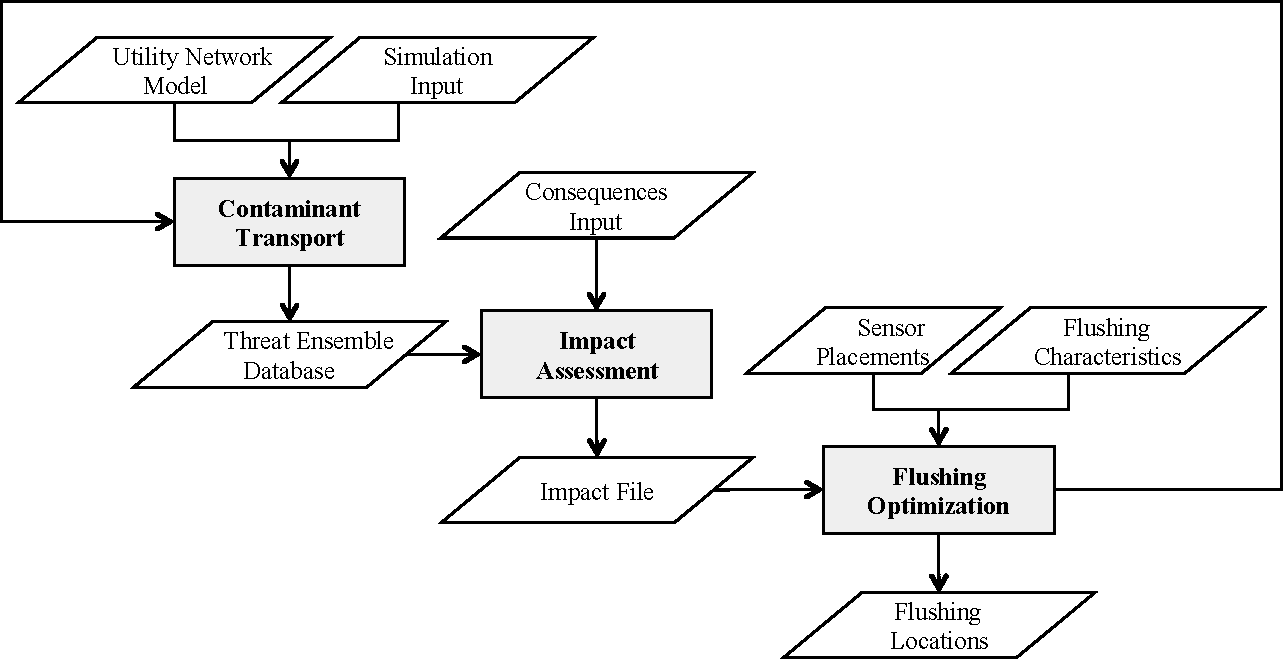
\includegraphics[scale=0.75]{graphics/flushing_flowchart.pdf}
  \caption{Flushing response simulation flowchart.}
  \label{fig:flushing-flowchart}
\end{figure}

\section{Flushing Formulation}\label{flushing_formulations}
The flushing problem formulation can be summarized 
as selecting a set of hydrant locations to flush and valves to close 
that minimizes the average impact of all contamination incidents 
given a set of potential hydrant locations to flush and valves to close. 
The mathematical formulation can be written as follows:
\begin{align}
\textrm{  minimize } \qquad &\dfrac{1}{A} \sum_{a \in {A}} d_{a,\max} \label{eqn:flushing} \\
\textrm{subject to } \qquad &\sum_{h\in H}y_{h} \leq H_{\max} \label{eq:flushing_2} \\
&\sum_{v\in V}y_{v} \leq V_{\max} \label{eq:flushing_3} \\  
&y_{h} \in \{0,1\} &&\forall h\in H \label{eq:flushing_4} \\
&y_{v} \in \{0,1\} &&\forall v\in V \label{eq:flushing_5}
\end{align}
where $A$ represents a set of contamination incidents, 
$d_{a,\max}$ defines the maximum impact of the contamination incident $a$, 
$H$ represents the set of potential hydrant locations,
$y_h$ is a binary variable which is 1 if node $h$ is selected as a flushing location, 
$H_{\max}$ is the maximum number of hydrant locations,
$V$ represents the set of potential valve locations,
$y_v$ is a binary variable which is 1 if node $v$ is selected as a valving location and 
$V_{\max}$ is the maximum number of valve locations. The maximum impact of a contamination
incident, $d_{a,\max}$, is the total impact across the entire network at the end of the simulation 
assuming that the contaminant was not detected by a sensor, and no interventions to reduce 
impacts were implemented. This value is found in the -1 entry of the impact file. 

For this problem, hydrants are assumed to be located at any user-defined nodes in the network. 
In addition, valves are assumed to be located on any user-defined pipes in the network.  

\section{Flushing Solvers}\label{flushing_solvers}
The flushing problem is solved through an iterative optimization process which 
selects different sets of hydrant and valve locations and evaluates their effectiveness
in minimizing the impact of a set of contamination incidents. Two optimization 
methods, an evolutionary algorithm and a network solver, are available in WST to solve this problem. 
Each solver is explained in more detail in the following subsections. 

\subsection{Evolutionary Algorithm}\label{coliny_ea}
The evolutionary algorithm (EA) included with DAKOTA, Coliny EA, is used in the 
optimization routine for the \code{flushing} subcommand. 
Additional information on DAKOTA/Coliny solvers can be found at 
\url{http://dakota.sandia.gov/docs/dakota/5.2/html-ref/index.html}
and in the DAKOTA user manual \citep{DakotaUserManual}.  
The random number generator used in Coliny EA is platform dependent.  
This can result in slight variations in the solution.

To design an EA, the parameter space for the optimization problem 
is first encoded into a string of numbers. This encoded 
representation of the problem is called a genetic string, where each 
element of the genetic string represents one parameter. 
When the EA is used with the \code{flushing} subcommand, the parameter space is defined by the number 
of flushing and valve closure locations. Each location is assigned a sequential 
integer that represents a feasible location within the EPANET network. The final EA solution 
is reported based on the EPANET node/pipe IDs.

The EA has several solver options that define how the EA evolves. These options can be set in the 
\code{[solver][options]} sections of the \code{flushing} WST configuration file and are specific to the Coliny EA solver. 
The EA evolves an initial genetic strings of size \code{[population\_size]} 
that is set based on \code{[initialization\_type]} using the following steps:
\begin{enumerate}
\item Evaluation: Evaluate the solution for each genetic string. This involves function 
calls to the \code{tevasim} and \code{sim2Impact} subcommands for each string to define the impact value.  
\item Breeding: Select two members of the population based on fitness. The 
probability of selection is based on \code{[fitness\_type]}.  
\item Crossover: Crossover two members based on \code{[crossover\_type]} and \code{[crossover\_rate]}.
\item Mutation: Mutate the two members based on \code{[mutation\_type]} and \code{[mutation\_rate]}.
\item Steps 2-4 are repeated until the entire population has been changed.
\item Replacement: After a new population is created, the old population is 
replaced by the current population while keeping the highest ranked string 
(elitist = 1 replacement option).
\end{enumerate}
Steps 1-6 are repeated until \code{[max\_iterations]} or \code{[max\_function\_evaluations]} criteria is met. 

\subsection{Network Solver}\label{coliny_statemachine}

The network solver used in WST is a network-constrained, derivative-free local search optimization algorithm. 
It is a discrete analog-to-pattern search. The allowable moves are to adjacent nodes (or pipes), rather than moves in the 
continuous space. This approach provides local refinement of candidate solutions. The valid moves include
removing a node (or pipe) location and replacing it with one anywhere in the network. Two forms of the network solver can be 
used: with and without initial starting points. The initial starting points are node (or pipe) locations in the network
in which the algorithm should begin its local search. If these points are not supplied to the algorithm, 
then it reduces to a greedy placement algorithm. Convergence is met when no remaining moves improve the solution.

\subsection{Flushing Optimization for Large Problems}

The iterative optimization process used for flushing requires numerous 
simulations of the network hydraulics and water quality. Computational run time depends on several factors, including 
the size of the network model, 
the number of possible contamination incidents, 
the number of feasible flushing locations 
and the solver options. For the network solver,the computational run time also depends on the network model
geometry surrounding the local search region. For large flushing optimization problems, several techniques can be used to 
decrease the computational run time. These options include running multiple instances of the underlying 
simulation in parallel, setting a stop time criteria and skeletonizing the network model.  

\subsubsection{Parallelization}

The Dakota coliny\_ea and StateMachineLS solvers both include an option to set 
the number of threads used to perform the simulations.   
This option is specified in \code{[solver][threads]}, as shown below. It should be 
set to the number of threads that are available for the simulation. The default value is 1.  
If an integer greater than 1 is specified, Dakota will run that many threads.
The expected efficiency of parallelization is nearly linear with the number of 
threads (up to the number of processor cores in the computer).

\begin{unknownListing}
solver:
  type: coliny_ea 
  threads: 2
\end{unknownListing}

\subsubsection{Stop time criteria}

If a solution needs to be identified within a certain amount of time, a simulation stop time 
criteria can be defined. This option causes the solver to terminate after a 
specified time, even if the underlying algorithm has not converged to an optimal solution.  
The stop time criteria is included with both the Dakota coliny\_ea and 
StateMachineLS solvers, and it is specified in \code{[solver][options][misc\_options]}, as 
shown below. The max\_time has to be given in seconds. As the optimization 
algorithms only check the elapsed time once per major iteration, the actual 
solver run time will be slightly longer than the specified maximum run time.  
When the optimization process is cut off prematurely, the best solution 
obtained so far is reported to the user.

\begin{unknownListing}
solver:
  type: StateMachineLS  
  options: 
    misc_options: "'max_time=10'"
\end{unknownListing}

\subsubsection{Skeletonization}

To reduce the size of the network model, possible contamination incidents and the number of 
feasible flushing locations, the user can skeletonize the problem and evaluate 
the results on the full network model. WST includes a utility script, spotSkeleton,  
that can be used to skeletonize network models (See Executable Files Section ~\ref{skelExecutable}).  
Network models are skeletonized based on a pipe diameter threshold. The executable, spotSkeleton,  
creates a new EPANET input (inp) file and a related map file.  
The map file associates the nodes in the skeletonized network model (upscaled nodes)  
to the nodes in the original network model (downscaled nodes). When  
working with a skeletonized network model, other aspects of the flushing problem also  
need to upscaled based on the skeletonization map. These include: the injection location(s)  
and strength of the contamination incident(s), the population at each node, the sensor  
placement, the feasible flushing locations and the initial points for the optimization  
solver. For example, if Nodes 1, 2, 3 and 4 in the original network model are  
represented by Node 2 in the skeletonized network model, then a sensor placed at  
Node 4 in the original network model should be placed at Node 2 in the skeletonized  
network model. 

After flushing optimization is run on the skeletonized network model, the  
solution can then be evaluated or refined using the original network model.  
To evaluate the current solution, the locations on the skeletonized network 
should be listed as the only feasible flushing locations  
in the original network model and the EVALUATE solver option should be used (See Example ~\ref{flushing_ex3}).   
To refine the current solution, downscale the locations on the skeletonized network
and use those original network nodes as the only feasible flushing locations  
in a second optimization. In this refinment, the solver type and  
solver options can be different for the first and second optimization.

\section{\code{flushing} Subcommand}

The \code{flushing} subcommand is executed using the following command line:
\begin{unknownListing}
wst flushing <configfile> 
\end{unknownListing}
where \code{configfile} is a WST configuration file in the YAML format. 

The \code{---help} option prints information about this subcommand, such as usage,
arguments and a brief description:
\begin{unknownListing}
wst flushing --help
\end{unknownListing}

\subsection{Configuration File}

The \code{flushing} subcommand generates a template configuration file using the following command line:

\begin{unknownListing}
wst flushing --template <configfile>
\end{unknownListing}

The \code{flushing} template configuration file is shown in Figure \ref{fig:flushing_template}.  
Brief descriptions of the options are included in the template after the \# sign.  

\begin{figure}[p!]
  \unknownInputListing{examples/flushing_config.yml}{}{1}{50}
  \caption{The \code{flushing} configuration template file.}
  \label{fig:flushing_template}
\end{figure}

\subsection{Configuration Options}

Full descriptions of the WST configuration options used by the \code{flushing} subcommand are listed below.
\begin{description}[topsep=0pt,parsep=0.5em,itemsep=-0.4em]
  \item[{network}]\hfill
  \begin{description}[topsep=0pt,parsep=0.5em,itemsep=-0.4em]
    \item[{epanet file}]\hfill
\\ The name of the EPANET 2.00.12 input (INP) file that defines the water distribution
                network model.
                
                Required input.
  \end{description}
  \item[{scenario}]\hfill
  \begin{description}[topsep=0pt,parsep=0.5em,itemsep=-0.4em]
    \item[{location}]\hfill
\\A list that describes the injection locations for the contamination scenarios.
                The options are: (1) ALL, which denotes all nodes (excluding tanks and reservoirs)
                as contamination injection locations; (2) NZD, which denotes all nodes with
                non-zero demands as contamination injection locations; or (3) an EPANET node ID, 
                which identifies a node as the contamination injection location. This allows 
                for an easy specification of single or multiple contamination scenarios.
                
                Required input unless a TSG or TSI file is specified.
    \item[{type}]\hfill
\\The injection type for the contamination scenarios. The options are MASS, CONCEN, FLOWPACED or SETPOINT. 
                See the EPANET 2.00.12 user manual for additional information about source types \citep{EPANETusermanual}.
                
                Required input unless a TSG or TSI file is specified.
    \item[{strength}]\hfill
\\The amount of contaminant injected into the network for the contamination scenarios.  
                If the type option is MASS, then the units for the strength are in mg/min. 
                If the type option is CONCEN, FLOWPACED or SETPOINT, then units are in mg/L.
                
                Required input unless a TSG or TSI file is specified.
    \item[{species}]\hfill
\\The name of the contaminant species injected into the network. This is the name of a single species. 
                It is required when using EPANET-MSX, since multiple species might be simulated, but
                only one is injected into the network. For cases where multiple contaminants are injected,
                a TSI file must be used.
                
                Required input for EPANET-MSX unless a TSG or TSI file is specified.
    \item[{start time}]\hfill
\\The injection start time that defines when the contaminant injection begins. 
                The time is given in minutes and is measured from the start of the simulation. 
                For example, a value of 60 represents an injection that starts at hour 1 of the simulation.
                
                Required input unless a TSG or TSI file is specified.
    \item[{end time}]\hfill
\\The injection end time that defines when the contaminant injection stops.				
                The time is given in minutes and is measured from the start of the simulation.
                For example, a value of 120 represents an injection that ends at hour 2 of the simulation.
                
                Required input unless a TSG or TSI file is specified.
    \item[{tsg file}]\hfill
\\The name of the TSG scenario file that defines the ensemble of contamination
                scenarios to be simulated. Specifying a TSG file will
                override the location, type, strength, species, start and end times options specified in
                the WST configuration file. The TSG file format is documented in File Formats Section \ref{formats_tsgFile}.
                
                Optional input.
    \item[{tsi file}]\hfill
\\The name of the TSI scenario file that defines the ensemble of contamination
                scenarios to be simulated. Specifying a TSI file will
                override the TSG file, as well as the location, type, strength, species, start and end time options specified in
                the WST configuration file. The TSI file format is documented in File Formats Section \ref{formats_tsiFile}.
                
                Optional input.
    \item[{signals}]\hfill
\\Name of file or directory with information to generate 
                or load signals. If a file is provided the list of inp tsg tuples
                 will be simulated and the information stored in signals files. If
                a directory with the signals files is specified, the signal files will
                be read and loaded in memory. This input is only valid for the uq
                subcommand and the grabsample subcommand with probability based formulations.

                Optional input.
    \item[{msx file}]\hfill
\\The name of the EPANET-MSX multi-species file that defines the multi-species reactions to
                be simulated using EPANET-MSX.
                
                Required input for EPANET-MSX.
    \item[{msx species}]\hfill
\\The name of the MSX species whose concentration profile will be saved by the EPANET-MSX simulation
                and used for later calculations.
                
                Required input for EPANET-MSX.
    \item[{merlion}]\hfill
\\A flag to indicate if the Merlion water quality
                simulator should be used. The options are true or false. 
                If an MSX file is provided, EPANET-MSX will be used.
                
                Required input, default = false.
  \end{description}
  \item[{impact}]\hfill
  \begin{description}[topsep=0pt,parsep=0.5em,itemsep=-0.4em]
    \item[{erd file}]\hfill
\\The name of the ERD database file that contains the 
                contaminant transport simulation results. It is 
                created by running the \code{tevasim} subcommand.
                Multiple ERD files (entered as a list, i.e., [<file1>, <file2>]) can be combined to
                generate a single impact file. This can be used to combine
                simulation results from different types of contaminants, in
                which the ERD files were generated from different
                TSG files.
                
                Required input.
    \item[{metric}]\hfill
\\The impact metric used to compute the impact file. Options
                include EC, MC, NFD, PD, PE, PK, TD or VC. One impact file 
                is created for each metric selected. These metrics are 
                defined in Section \ref{impact_measures}.
                
                Required input.
    \item[{tai file}]\hfill
\\The name of the TAI file that contains health impact information. 
                The TAI file format is documented in File Formats Section \ref{formats_taiFile}.
                
                Required input if a public health metric is used (PD, PE or PK).
    \item[{response time}]\hfill
\\The number of minutes that are needed to respond to the
                detection of a contaminant. This represents the time that it takes
                a water utility to stop the spread of the contaminant in the network and 
                eliminate the consumption of contaminated water. As the response time increases,
                the impact increases because the contaminant affects the network
                for a greater length of time.  
                
                Required input, default = 0 minutes.
    \item[{detection limit}]\hfill
\\The minimum concentration that must be exceeded before a sensor can detect a contaminant.
                There must be one threshold for each ERD file. The units of
                these detection limits depend on the units of the contaminant
                simulated for each ERD file (e.g., number of cells of a
                biological agent).  
                
                Required input, default = 0.
    \item[{detection confidence}]\hfill
\\The number of sensors that must detect an incident before
                the impacts are calculated.  
                
                Required input, default = 1 sensor.
  \end{description}
  \item[{flushing}]\hfill
  \begin{description}[topsep=0pt,parsep=0.5em,itemsep=-0.4em]
    \item[{detection}]\hfill
\\The sensor network design used to detect contamination scenarios. The
                sensor locations are used to compute a detection time for each 
                contamination scenario. The options are a list of 
                EPANET node IDs or a file name which contains a list of EPANET node IDs.
                
                Required input.
    \item[{flush nodes}]\hfill
    \begin{description}[topsep=0pt,parsep=0.5em,itemsep=-0.4em]
      \item[{feasible nodes}]\hfill
\\A list that defines the nodes in the network that can be flushed. 
                The options are: (1) ALL, which specifies all nodes as feasible flushing locations;
                (2) NZD, which specifies all non-zero demand nodes as feasible flushing locations;
                (3) NONE, which specifies no nodes as feasible flushing locations;
                (4) a list of EPANET node IDs, which identifies specific nodes as feasible flushing locations; or
                (5) a filename, which references a space or comma separated file containing a list of 
                specific nodes as feasible flushing locations.
                
                Required input, default = ALL.
      \item[{infeasible nodes}]\hfill
\\A list that defines the nodes in the network that cannot be flushed. 
                The options are: (1) ALL, which specifies all nodes as infeasible flushing locations;
                (2) NZD, which specifies all non-zero demand nodes as infeasible flushing locations;
                (3) NONE, which specifies no nodes as infeasible flushing locations;
                (4) a list of EPANET node IDs, which identifies specific nodes as infeasible flushing locations; or
                (5) a filename, which references a space or comma separated file containing a list of 
                specific nodes as infeasible flushing locations. 
                
                Optional input, default = NONE.
      \item[{max nodes}]\hfill
\\The maximum number of node locations that can be flushed simultaneously in the
                network. The value is a nonnegative integer or a list of
                nonnegative integers. When a list is specified, the optimization
                will be performed for each number in this list. For example, a value of 
                3 means that a maximum of 3 node will be identified as flushing locations 
                during the optimization process.
                
                Required input.
      \item[{rate}]\hfill
\\The flushing rate for each node location to be flushed. A new demand pattern 
                will be created using this rate for the node. The value is a nonnegative integer. 
                For example, a value of 800 means that an additional demand of 800 gpm is applied 
                at a particular node. This rate is applied to all flushing locations identified 
                in the optimization process.
                
                Required input.
      \item[{response time}]\hfill
\\The time in minutes between the detection of a contamination incident and 
                the start of flushing. The value is a nonnegative integer. For example, 
                a value of 120 represents a 120 minutes or a 2 hour delay between 
                the time of detection and the start of flushing.
                
                Required input.
      \item[{duration}]\hfill
\\The length of time in minutes that flushing will be simulated at a particular node. 
                The value is a nonnegative integer. For example, a value of 240 means that  
                flushing would be simulated at a particular node for 4 hours. This duration 
                is applied to all flushing locations identified in the optimization process.
                
                Required input.
    \end{description}
    \item[{close valves}]\hfill
    \begin{description}[topsep=0pt,parsep=0.5em,itemsep=-0.4em]
      \item[{feasible pipes}]\hfill
\\A list that defines the pipes in the network that can be closed. 
                The options are: (1) ALL, which specifies all pipes as feasible pipes to close;
                (2) DIAM min max, which specifies all pipes with a specific diameter as feasible pipes to close;
                (3) NONE, which specifies no pipes as feasible pipes to close;
                (4) a list of EPANET pipe IDs, which identifies specific pipes as feasible pipes to close; or
                (5) a filename, which references a space or comma separated file containing a list of 
                specific pipes as feasible pipes to close. 
                
                Required input, default = ALL.
      \item[{infeasible pipes}]\hfill
\\A list that defines the pipes in the network that cannot be closed. 
                The options are: (1) ALL, which specifies all pipes as infeasible pipes to close;
                (2) DIAM min max, which specifies all pipes with a specific diameter as infeasible pipes to close;
                (3) NONE, which specifies no pipes as infeasible pipes to close;
                (4) a list of EPANET pipe IDs, which identifies specific pipes as infeasible pipes to close; or
                (5) a filename, which references a space or comma separated file containing a list of 
                specific pipes as infeasible pipes to close. 
                
                Optional input, default = NONE.
      \item[{max pipes}]\hfill
\\The maximum number of pipes that can be closed simultaneously in the
                network. The value must be a nonnegative integer or a list of
                nonnegative integers. When a list is specified, the optimization
                will be performed for each number in this list. For example, a value of 
                2 means that a maximum of 2 pipes to close will be identified 
                during the optimization process.
                
                Required input.
      \item[{response time}]\hfill
\\The time in minutes between the detection of a contamination incident and 
                closing pipes. The value is a nonnegative integer. For example, 
                a value of 120 would represent a 120 minutes or a 2 hour delay between 
                the time of detection and the start of pipe closures.
                
                Required input.
    \end{description}
  \end{description}
  \item[{solver}]\hfill
  \begin{description}[topsep=0pt,parsep=0.5em,itemsep=-0.4em]
    \item[{type}]\hfill
\\The solver type. Each component of WST
				(e.g., sensor placement, flushing response, booster 
				placement) has different 
				solvers available. More specific details are provided in 
				the subcommand's chapter.
                
                Required input.
    \item[{options}]\hfill
\\A list of options associated with a specific solver type. More
            information on the options available for a specific solver
            is provided in the solver's documentation. The Getting
            Started Section \ref{dependencies} provides links to the
            different solvers.
            
            Optional input.
    \item[{threads}]\hfill
\\The maximum number of threads or function evaluations the solver is
                allowed to use.  This option is not available to all solvers or all analyses.
                
                Optional input.
    \item[{logfile}]\hfill
\\The name of a file to output the results of the solver.
                
                Optional input.
    \item[{verbose}]\hfill
\\The solver verbosity level.
                
                Optional input, default = 0 (lowest level).
    \item[{initial points}]\hfill
    \begin{description}[topsep=0pt,parsep=0.5em,itemsep=-0.4em]
      \item[{nodes}]\hfill
\\A list of node locations (EPANET IDs) to begin the optimization
        process. Currently, this option is only supported for the
        network solver used in the flushing and booster\_msx
        subcommands. This input causes an error for other subcommands.
        
        Optional input.
      \item[{pipes}]\hfill
\\A list of pipe locations (EPANET IDs) to begin the optimization
        process. Currently, this option is only supported for the
        network solver used in the flushing subcommand. This input causes an error for other subcommands.
        
        Optional input.
    \end{description}
  \end{description}
  \item[{configure}]\hfill
  \begin{description}[topsep=0pt,parsep=0.5em,itemsep=-0.4em]
    \item[{output prefix}]\hfill
\\The prefix used for all output files.
                
                Required input.
    \item[{output directory}]\hfill
      \\The output directory to store the results.
    \item[{debug}]\hfill
\\The debugging level (0 or 1) that indicates the amount of debugging 
                information printed to the screen, log file and output yml file. 
                
                Optional input, default = 0 (lowest level).
  \end{description}
\end{description}


In addition to these standard WST configuration options, the solver block can define 
an evaluation option. To evaluate the flushing response without solving the 
optimization problem, the solver type can be set as EVALUATE. This option allows a 
set of flushing locations to be evaluated against a different contamination 
scenario than the one for which it was designed. 

The solver block can also define specific options for the optimization solver. 
The solver options should be modified according to the specific optimization problem. 
If the options are not set in the solver block, then the default values for these options are used. 
The two solvers available in the \code{flushing} subcommand each have their own options. 
The EA solver has numerous options which can be defined. Additional information on the options available
for the EA solver can found in the DAKOTA user manual \citep{DakotaUserManual}. 
An example of the EA solver options are listed below.

\begin{unknownListing}
solver:
  type: coliny_ea
  options: 
    crossover_rate: 0.8
    crossover_type: uniform
    fitness_type: linear_rank
    initialization_type: unique_random
    max_function_evaluations: 30000
    max_iterations: 1000
    mutation_rate: 1
    mutation_type: offset_uniform
    population_size: 50
    seed: 11011011
\end{unknownListing}

The network solver has two options that can be set in the solver block of the configuration file. 
\begin{unknownListing}
solver:  
  type: StateMachineLS
  options:
    verbosity: 2
    max_fcn_evaluations: 0
\end{unknownListing}

\subsection{Subcommand Output}
The \code{flushing} subcommand creates a YAML file called <output prefix>flushing\_output.yml 
that contains an optimized set of node locations (EPANET node IDs) to flush, 
an optimized set of pipe locations (EPANET pipe IDs) to close,
the final impact metric, the run date and CPU time. 
The log file called <output prefix>flushing\_output.log contains basic debugging information.
A visualization YAML configuration file named <output prefix>flushing\_output\_vis.yml is also created.
The \code{visualization} subcommand is automatically run using this YAML file.

\section{Flushing Response Examples}\label{flushing_example}
To demonstrate the two different solvers available in the \code{flushing} subcommand, 
two examples are presented. Both examples have the same characteristics in terms 
of the contamination scenario and flushing parameters. EPANET Example Network 3 (Net3.inp)
is the network used and the contamination scenario is an hour long injection at 
node 101 beginning at hour 3 in the simulation. A maximum of three hydrants can be flushed 
for a duration of eight hours at a rate 800 gal/min. The option to close pipes/valves was 
not included in these analyses. The impact metric being minimized is population exposed (PE). 
In addition, the third and forth examples are provided to demonstrate the evaluate and stop time
criteria options, respectively.

\subsection{Example 1}

The first example uses the EA solver (coliny\_ea) with the parallization option enabled 
and the configuration file, flushing\_ex1.yml, is shown in Figure \ref{fig:flushing_ex1}. This example
has the \code{[solver][threads]} option set to 2 threads. Please note: 
if the computer used to execute the example only has one thread, change the \code{[solver][threads]} 
option to 1 instead of 2.

\begin{figure}[h]
  \unknownInputListing{../../examples/flushing_ex1.yml}{}{1}{55}
  \caption{The \code{flushing} configuration file for example 1.}
  \label{fig:flushing_ex1}
\end{figure}

The example can be executed using the following command line:

\begin{unknownListing}
wst flushing flushing_ex1.yml
\end{unknownListing}

The YAML output file, Net3flushing\_output.yml, for example 1 
is shown in Figure \ref{fig:flushing_ex1_yml}. The EA selected to 
flush nodes 113, 191 and 197 for a PE impact value of 5292. The CPU time 
was approximately 6 minutes using 2 threads. 
Since the random number generator used in the EA solver is platform dependent,   
the solution can be slightly different if the example is executed on a computer with Windows.

\begin{figure}[h]
  \unknownInputListing{examples/flushing/flushing_ex1_output.yml}{}{1}{11}
  \caption{The \code{flushing} YAML output file for example 1.}
  \label{fig:flushing_ex1_yml}
\end{figure}

% \FloatBarrier 
\subsection{Example 2}

The second example uses the network solver (StateMachineLS) 
without initial points and the configuration file, flushing\_ex2.yml, 
is shown in Figure \ref{fig:flushing_ex2}. 

\begin{figure}[h]
  \unknownInputListing{../../examples/flushing_ex2.yml}{}{1}{45}
  \caption{The \code{flushing} configuration file for example 2.}
  \label{fig:flushing_ex2}
\end{figure}

The example can be executed using the following command line:

\begin{unknownListing}
wst flushing flushing_ex2.yml
\end{unknownListing}

The YAML output file, Net3flushing\_output.yml, for example 2 is shown 
in Figure \ref{fig:flushing_ex2_yml}. The network solver selected to 
flush nodes 101, 103 and 109 for a PE impact metric of 4919. The CPU time 
was approximately 2 minutes.

\begin{figure}[h]
  \unknownInputListing{examples/flushing/flushing_ex2_output.yml}{}{1}{11}
  \caption{The \code{flushing} YAML output file for example 2.}
  \label{fig:flushing_ex2_yml}
\end{figure}

Examining the output files from the two examples shows that the optimization
solvers identified different solutions. As EAs are not guaranteed to find the 
optimal solution, these results are not unexpected. In addition, the CPU times 
to obtain the solutions are different. The EA solution took about 6 minutes 
to obtained using 2 threads, while the network solver solution was achieved in approximately 2 minutes.

\subsection{Example 3}\label{flushing_ex3}

The third example uses the evaluate option and the configuration 
file, flushing\_ex3.yml, is shown in Figure \ref{fig:flushing_ex3}. 
In this example, the same contamination scenario is used but only two 
(2) flushing locations are evaluated in terms of reducing the PE impact 
metric. The flushing locations being evaluated are nodes 101 and 127. 

\begin{figure}[h]
  \unknownInputListing{../../examples/flushing_ex3.yml}{}{1}{44}
  \caption{The \code{flushing} configuration file for example 3.}
  \label{fig:flushing_ex3}
\end{figure}

The example can be executed using the following command line:

\begin{unknownListing}
wst flushing flushing_ex3.yml
\end{unknownListing}

The YAML output file, Net3flushing\_output.yml, for example 3 is shown 
in Figure \ref{fig:flushing_ex3_yml}. These two flushing locations 
resulted in a PE impact metric of 10,759. Compared to the results from 
example 2, the PE impact metric is much larger since only two flushing 
locations are used instead of three. The evaluate option can be used to compare 
the impact metrics obtained from various flushing location combinations. 

\begin{figure}[h]
  \unknownInputListing{examples/flushing/flushing_ex3_output.yml}{}{1}{11}
  \caption{The \code{flushing} YAML output file for example 3.}
  \label{fig:flushing_ex3_yml}
\end{figure}

\subsection{Example 4}

The fourth example demonstrates the stop time option and uses almost the same configuration file as example 2. 
The configuration file, flushing\_ex4.yml, is shown in Figure \ref{fig:flushing_ex4}, in which 
the stop criteria option is enabled using the \code{[solver][options][misc\_options]} option set to "'max\_time=30'".

\begin{figure}[h]
  \unknownInputListing{../../examples/flushing_ex4.yml}{}{1}{46}
  \caption{The \code{flushing} configuration file for example 4.}
  \label{fig:flushing_ex4}
\end{figure}

The example can be executed using the following command line:

\begin{unknownListing}
wst flushing flushing_ex4.yml
\end{unknownListing}

The YAML output file, Net3flushing\_output.yml, for example 4 
is shown in Figure \ref{fig:flushing_ex4_yml}. The network solver selected to 
flush node 105 for a PE impact value of 9676. The CPU time was 45 seconds, 
which is greater than the stop time criteria since it is only checked periodically. 
The flushing solution was different than the solution obtained from example 2, 
since the stop time option was not used and it executed the optimization process to completion. 

\begin{figure}[h]
  \unknownInputListing{examples/flushing/flushing_ex4_output.yml}{}{1}{11}
  \caption{The \code{flushing} YAML output file for example 4.}
  \label{fig:flushing_ex4_yml}
\end{figure}



  \chapter{Booster Station Placement}
  \label{chap:booster}
  Disinfection booster stations are commonly used throughout water distribution networks 
to maintain drinking water standards. Disinfectants degrade as they move through the 
system and booster stations, designed to inject disinfectant at strategic locations, 
help maintain residual levels. Booster stations can also be placed with 
water security objectives in mind. WST includes two booster subcommands, \code{booster\_msx} 
and \code{booster\_mip} that are 
designed to place booster stations to minimize the impact of a contamination incident. 
These subcommands use different approaches to model the reaction dynamics between 
a contaminant and disinfectant. 

The \code{booster\_msx} subcommand uses EPANET-MSX to 
simulate the reaction dynamics between the contaminant and disinfectant. 
A flowchart representation of the \code{booster\_msx} subcommand is shown 
in Figure \ref{fig:booster_msx_flowchart}. The \code{booster\_msx} subcommand employs 
an iterative process that combines contaminant transport, impact assessment 
and optimization. The optimization process identifies a set of booster station locations 
where disinfectant is injected. The contaminant and disinfectant injections and their 
reaction dynamics are simulated in the contaminant transport 
process and the effectiveness of the booster injections are evaluated based upon 
the impact assessment process. Since the \code{booster\_msx} subcommand relies 
on the \code{tevasim} and \code{sim2Impact} subcommands, their required input 
is also required for the \code{booster\_msx} subcommand. Additionally, the sensor network 
design used to detect the contamination incident(s) and the booster station characteristics 
are required inputs. The utility network model is defined by a EPANET 2.00.12 INP file, 
while the rest of the input can be specified in the \code{booster\_msx} WST configuration file.

\begin{figure}[h]
  \centering
  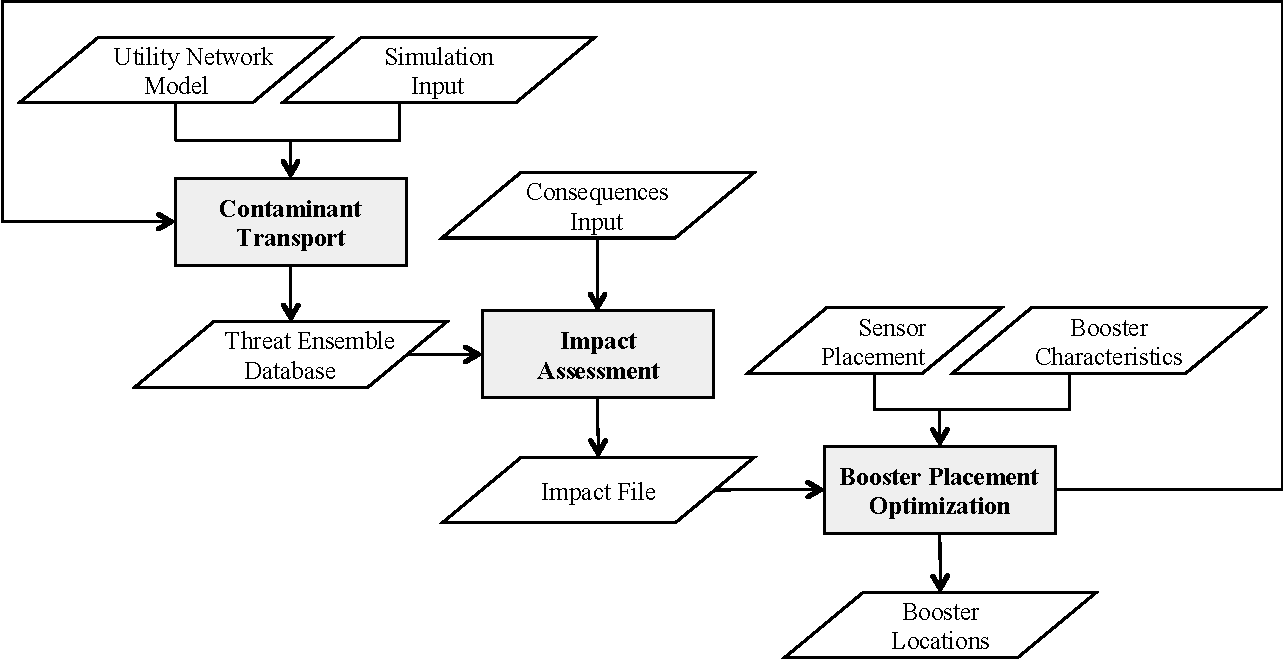
\includegraphics[scale=0.75]{graphics/booster_msx_flowchart.pdf}
  \caption{Multi-species reaction booster placement flowchart.}
  \label{fig:booster_msx_flowchart}
\end{figure}

The \code{booster\_mip} 
subcommand uses the linear water quality model Merlion and assumes the reaction dynamics between the contaminant and 
disinfectant can be approximated by a neutralization or limiting reagent reaction model.
A flowchart representation of the \code{booster\_mip} subcommand is shown in Figure \ref{fig:booster_mip_flowchart}. 
The utility network model is defined by a EPANET 2.00.12 INP file. Additional input specified in the \code{booster\_mip} WST 
configuration file are the contamination scenarios, the sensor network design used to detect 
the contamination incident(s) and the booster station characteristics. 

\begin{figure}[h]
  \centering
  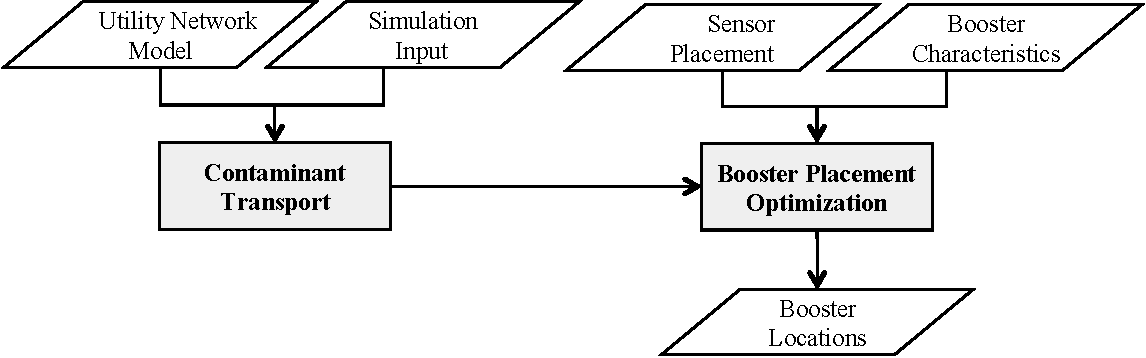
\includegraphics[scale=0.75]{graphics/booster_mip_flowchart.pdf}
  \caption{MIP booster placement flowchart.}
  \label{fig:booster_mip_flowchart}
\end{figure}

\section{Booster Placement Using Multi-species Reaction}\label{booster_msx_formulations}

The \code{booster\_msx} subcommand uses optimization methods integrated 
with EPANET-MSX to evaluate booster placements using multi-species reaction dynamics between 
the contaminant and disinfectant. The booster station placement problem formulation 
selects a set of booster station locations that minimizes the average impact 
of all contamination incidents given a set of potential booster stations that 
inject a disinfecting agent. The mathematical formulation can be written as follows:
\begin{align}
\textrm{  minimize } \qquad & \dfrac{1}{A} \sum_{a \in {A}}d_{a,\max} \label{eqn:booster_msx} \\
\textrm{subject~to } \qquad &\sum_{b\in B}y_{b} \leq B_{\max} \label{eq:booster_msx_2} \\
&y_{b} \in \{0,1\} &&\forall b\in B \label{eq:booster_msx_3}
\end{align}
where ${A}$ represents a set of contamination incidents, 
$d_{a,\max}$ defines the maximum impact of the contamination incident $a$, 
$B$ represents the set of potential booster station locations,
$y_b$ is a binary variable which is 1 if node $b$ is selected as a booster station location 
and $B_{\max}$ is the maximum number of booster station locations. 
The maximum impact of a contamination incident, $d_{a,\max}$, is the total impact 
across the entire network at the end of the simulation assuming that the 
contaminant was not detected by a sensor, and no interventions to reduce 
impacts were implemented. This value is found in the -1 entry of the impact file. 
For this problem, it is assumed that booster stations can be located at any 
user-defined nodes in the network.

\subsection{Booster MSX Solvers}
The multi-species booster station placement problem is solved through an iterative optimization process which 
selects different sets of booster station locations and evaluates their effectiveness
in minimizing the impact of a set of contamination incidents. Two optimization 
methods, an evolutionary algorithm and a network solver, are available in WST to solve this problem. 
Each solver is explained in more detail in the following subsections. 

\subsubsection{Evolutionary Algorithm}\label{boostermsx_coliny_ea}
The evolutionary algorithm (EA) included with DAKOTA, Coliny EA, is used in the 
optimization routine for the \code{booster\_msx} subcommand. 
Additional information on DAKOTA/Coliny solvers can be found at 
\url{http://dakota.sandia.gov/docs/dakota/5.2/html-ref/index.html}
and in the DAKOTA user manual \citep{DakotaUserManual}.
The random number generator used in Coliny EA is platform dependent.  
This can result in slight variations in the solution.

To design an EA, the parameter space for the optimization problem is first 
encoded into a string of numbers. This encoded representation of the problem 
is called a genetic string, where each element of the genetic string represents 
one parameter. When the EA is used with \code{booster\_msx}\, the parameter space 
is defined by the number of booster station locations. Each location is assigned a sequential 
integer that represents a feasible location within the EPANET network. The final EA solution is 
translated to represent EPANET node IDs.

The EA has several solver options that define how the EA evolves. These options can be set in the 
\code{[solver][options]} sections of the \code{booster\_msx} WST configuration file and are specific to the Coliny EA solver. 
The EA evolves an initial genetic strings of size \code{[population\_size]} that is 
set based on \code{[initialization\_type]} using the following steps:
\begin{enumerate}
\item Evaluation: Evaluate the solution for each genetic string. This involves function 
calls to the \code{tevasim} and \code{sim2Impact} subcommands for each string to define the fitness score.  
\item Breeding: Select two members of the population based on fitness. The 
probability of selection is based on \code{[fitness\_type]}.  
\item Crossover: Crossover two members based on \code{[crossover\_type]} and \code{[crossover\_rate]}. 
\item Mutation: Mutate the two members based on \code{[mutation\_type]} and \code{[mutation\_rate]}.
\item Steps 2-4 are repeated until the entire population has been changed.
\item Replacement: After a new population is created, the old population is 
replaced by the current population while keeping the highest ranked string 
(elitist = 1 replacement option).
\end{enumerate}
Steps 1-6 are repeated until \code{[max\_iterations]} or \code{[max\_function\_evaluations]} criteria is met. 

\subsubsection{Network Solver}\label{boostermsx_coliny_statemachine}

The network solver used in WST is a network-constrained, derivative-free local search optimization algorithm. 
It is a discrete analog-to-pattern search. The allowable moves are to adjacent nodes, rather than moves in the 
continuous space. This approach provides local refinement of candidate solutions. The valid moves include
removing a node location and replacing it with one anywhere in the network. Two forms of the network solver can be 
used: with and without initial starting points. The initial starting points are node locations in the network
in which the algorithm should begin its local search. If these points are not supplied to the algorithm, 
then it reduces to a greedy placement algorithm. Convergence is met when no remaining moves improve the solution.

\if 0
\subsubsection{Parallelization}

The Dakota coliny\_ea and StateMachineLS solvers both include an option to set 
the number of threads used to perform the simulations.   
This option is specified in \code{[solver][threads]}, as shown below. It should be 
set to the number of threads that are available for the simulation. The default value is 1.  
If an integer greater than 1 is specified, Dakota will run that many threads.
The expected efficiency of parallelization is nearly linear with the number of 
threads (up to the number of processor cores in the computer).

\begin{unknownListing}
solver:
  type: coliny_ea 
  threads: 2
\end{unknownListing}

\subsubsection{Stop time criteria}

If a solution needs to be identified within a certain amount of time, a simulation stop time 
criteria can be defined. This option causes the solver to terminate after a 
specified time, even if the underlying algorithm has not converged to an optimal solution.  
The stop time criteria is included with both the Dakota coliny\_ea and 
StateMachineLS solvers, and it is specified in \code{[solver][options][misc\_options]}, as 
shown below. The max\_time has to be given in seconds. As the optimization 
algorithms only check the elapsed time once per major iteration, the actual 
solver run time will be slightly longer than the specified maximum run time.  
When the optimization process is cut off prematurely, the best solution 
obtained so far is reported to the user.

\begin{unknownListing}
solver:
  type: StateMachineLS  
  options: 
    misc_options: "'max_time=10'"
\end{unknownListing}

% \subsubsection{Skeletonization}

% To reduce the size of the network model, possible contamination incidents and the number of 
% feasible booster station locations, the user can skeletonize the problem and evaluate 
% the results on the full network model. WST includes a utility script, spotSkeleton,  
% that can be used to skeletonize network models (See Executable Files Section ~\ref{skelExecutable}).  
% Network models are skeletonized based on a pipe diameter threshold. The executable, spotSkeleton,  
% creates a new EPANET input (inp) file and a related map file.  
% The map file associates the nodes in the skeletonized network model (upscaled nodes)  
% to the nodes in the original network model (downscaled nodes). When  
% working with a skeletonized network model, other aspects of the booster station problem also  
% need to upscaled based on the skeletonization map. These include: the injection location(s)  
% and strength of the contamination incident(s), the population at each node, the sensor  
% placement, the feasible booster station locations, and the initial points for the optimization  
% solver. For example, if Nodes 1, 2, 3 and 4 in the original network model are  
% represented by Node 2 in the skeletonized network model, then a sensor placed at  
% Node 4 in the original network model should be placed at Node 2 in the skeletonized  
% network model. 

% After booster station optimization is run on the skeletonized network model, the  
% solution can then be evaluated or refined using the original network model.  
% To evaluate the current solution, the locations on the skeletonized network 
% should be listed as the only feasible booster station locations  
% in the original network model and the EVALUATE solver option should be used (See Example ~\ref{booster_ex2}}).   
% To refine the current solution, downscale the locations on the skeletonized network
% and use those original network nodes as the only feasible booster station locations  
% in a second optimization. In this refinment, the solver type and  
% solver options can be different for the first and second optimization.
\fi

\subsection{\code{booster\_msx} Subcommand}

The \code{booster\_msx} subcommand is executed using the following command line:
\begin{unknownListing}
wst booster_msx <configfile> 
\end{unknownListing}
where \code{configfile} is a WST configuration file in the YAML format. 

The \code{---help} option prints information about this subcommand, such as usage,
arguments and a brief description:
\begin{unknownListing}
wst booster_msx --help
\end{unknownListing}

\subsubsection{Configuration File}

The \code{booster\_msx} subcommand generates a template configuration file using the following command line:

\begin{unknownListing}
wst booster_msx --template <configfile>
\end{unknownListing}

The \code{booster\_msx} template configuration file is shown in Figure \ref{fig:booster_msx_template}.  
Brief descriptions of the options are included in the template after the \# sign.  

\begin{figure}[p!]
  \unknownInputListing{examples/booster_msx_config.yml}{}{1}{47}
  \caption{The \code{booster\_msx} configuration template file.}
  \label{fig:booster_msx_template}
\end{figure}

\subsubsection{Configuration Options}

Full descriptions of the WST configuration options used by the \code{booster\_msx} subcommand are listed below.
\begin{description}[topsep=0pt,parsep=0.5em,itemsep=-0.4em]
  \item[{network}]\hfill
  \begin{description}[topsep=0pt,parsep=0.5em,itemsep=-0.4em]
    \item[{epanet file}]\hfill
\\ The name of the EPANET 2.00.12 input (INP) file that defines the water distribution
                network model.
                
                Required input.
  \end{description}
  \item[{scenario}]\hfill
  \begin{description}[topsep=0pt,parsep=0.5em,itemsep=-0.4em]
    \item[{location}]\hfill
\\A list that describes the injection locations for the contamination scenarios.
                The options are: (1) ALL, which denotes all nodes (excluding tanks and reservoirs)
                as contamination injection locations; (2) NZD, which denotes all nodes with
                non-zero demands as contamination injection locations; or (3) an EPANET node ID, 
                which identifies a node as the contamination injection location. This allows 
                for an easy specification of single or multiple contamination scenarios.
                
                Required input unless a TSG or TSI file is specified.
    \item[{type}]\hfill
\\The injection type for the contamination scenarios. The options are MASS, CONCEN, FLOWPACED or SETPOINT. 
                See the EPANET 2.00.12 user manual for additional information about source types \citep{EPANETusermanual}.
                
                Required input unless a TSG or TSI file is specified.
    \item[{strength}]\hfill
\\The amount of contaminant injected into the network for the contamination scenarios.  
                If the type option is MASS, then the units for the strength are in mg/min. 
                If the type option is CONCEN, FLOWPACED or SETPOINT, then units are in mg/L.
                
                Required input unless a TSG or TSI file is specified.
    \item[{species}]\hfill
\\The name of the contaminant species injected into the network. This is the name of a single species. 
                It is required when using EPANET-MSX, since multiple species might be simulated, but
                only one is injected into the network. For cases where multiple contaminants are injected,
                a TSI file must be used.
                
                Required input for EPANET-MSX unless a TSG or TSI file is specified.
    \item[{start time}]\hfill
\\The injection start time that defines when the contaminant injection begins. 
                The time is given in minutes and is measured from the start of the simulation. 
                For example, a value of 60 represents an injection that starts at hour 1 of the simulation.
                
                Required input unless a TSG or TSI file is specified.
    \item[{end time}]\hfill
\\The injection end time that defines when the contaminant injection stops.				
                The time is given in minutes and is measured from the start of the simulation.
                For example, a value of 120 represents an injection that ends at hour 2 of the simulation.
                
                Required input unless a TSG or TSI file is specified.
    \item[{tsg file}]\hfill
\\The name of the TSG scenario file that defines the ensemble of contamination
                scenarios to be simulated. Specifying a TSG file will
                override the location, type, strength, species, start and end times options specified in
                the WST configuration file. The TSG file format is documented in File Formats Section \ref{formats_tsgFile}.
                
                Optional input.
    \item[{tsi file}]\hfill
\\The name of the TSI scenario file that defines the ensemble of contamination
                scenarios to be simulated. Specifying a TSI file will
                override the TSG file, as well as the location, type, strength, species, start and end time options specified in
                the WST configuration file. The TSI file format is documented in File Formats Section \ref{formats_tsiFile}.
                
                Optional input.
    \item[{signals}]\hfill
\\Name of file or directory with information to generate 
                or load signals. If a file is provided the list of inp tsg tuples
                 will be simulated and the information stored in signals files. If
                a directory with the signals files is specified, the signal files will
                be read and loaded in memory. This input is only valid for the uq
                subcommand and the grabsample subcommand with probability based formulations.

                Optional input.
    \item[{msx file}]\hfill
\\The name of the EPANET-MSX multi-species file that defines the multi-species reactions to
                be simulated using EPANET-MSX.
                
                Required input for EPANET-MSX.
    \item[{msx species}]\hfill
\\The name of the MSX species whose concentration profile will be saved by the EPANET-MSX simulation
                and used for later calculations.
                
                Required input for EPANET-MSX.
    \item[{merlion}]\hfill
\\A flag to indicate if the Merlion water quality
                simulator should be used. The options are true or false. 
                If an MSX file is provided, EPANET-MSX will be used.
                
                Required input, default = false.
  \end{description}
  \item[{impact}]\hfill
  \begin{description}[topsep=0pt,parsep=0.5em,itemsep=-0.4em]
    \item[{erd file}]\hfill
\\The name of the ERD database file that contains the 
                contaminant transport simulation results. It is 
                created by running the \code{tevasim} subcommand.
                Multiple ERD files (entered as a list, i.e., [<file1>, <file2>]) can be combined to
                generate a single impact file. This can be used to combine
                simulation results from different types of contaminants, in
                which the ERD files were generated from different
                TSG files.
                
                Required input.
    \item[{metric}]\hfill
\\The impact metric used to compute the impact file. Options
                include EC, MC, NFD, PD, PE, PK, TD or VC. One impact file 
                is created for each metric selected. These metrics are 
                defined in Section \ref{impact_measures}.
                
                Required input.
    \item[{tai file}]\hfill
\\The name of the TAI file that contains health impact information. 
                The TAI file format is documented in File Formats Section \ref{formats_taiFile}.
                
                Required input if a public health metric is used (PD, PE or PK).
    \item[{response time}]\hfill
\\The number of minutes that are needed to respond to the
                detection of a contaminant. This represents the time that it takes
                a water utility to stop the spread of the contaminant in the network and 
                eliminate the consumption of contaminated water. As the response time increases,
                the impact increases because the contaminant affects the network
                for a greater length of time.  
                
                Required input, default = 0 minutes.
    \item[{detection limit}]\hfill
\\The minimum concentration that must be exceeded before a sensor can detect a contaminant.
                There must be one threshold for each ERD file. The units of
                these detection limits depend on the units of the contaminant
                simulated for each ERD file (e.g., number of cells of a
                biological agent).  
                
                Required input, default = 0.
    \item[{detection confidence}]\hfill
\\The number of sensors that must detect an incident before
                the impacts are calculated.  
                
                Required input, default = 1 sensor.
  \end{description}
  \item[{booster msx}]\hfill
  \begin{description}[topsep=0pt,parsep=0.5em,itemsep=-0.4em]
    \item[{detection}]\hfill
\\The sensor network design used to detect contamination scenarios. The
                sensor locations are used to compute a detection time for each 
                contamination scenario in the TSG file. The options are a list of 
                EPANET node IDs or a file name which contains a list of EPANET node IDs.
                
                Required input.
    \item[{toxin species}]\hfill
\\The name of the contaminant species that is injected in each
                contamination scenario. This is the species that interacts with the 
                injected disinfectant and whose impact is going to be minimized.
                
                Required input.
    \item[{decon species}]\hfill
\\The name of the decontaminant or disinfectant species that is injected from the 
                booster stations.
                
                Required input.
    \item[{feasible nodes}]\hfill
\\A list that defines nodes that can be considered for the booster station placement problem.
                The options are: (1) ALL, which specifies all nodes as feasible booster station locations;
                (2) NZD, which specifies all non-zero demand nodes as feasible booster station locations;
                (3) NONE, which specifies no nodes as feasible booster station locations;
                (4) a list of EPANET node IDs, which identifies specific nodes as feasible booster station locations; or
                (5) a filename, which references a space or comma separated file containing a list of 
                specific nodes as feasible booster station locations.
                
                Required input, default = ALL.
    \item[{infeasible nodes}]\hfill
\\A list that defines nodes that cannot be considered for the booster station placement problem.
                The options are: (1) ALL, which specifies all nodes as infeasible booster station locations;
                (2) NZD, which specifies non-zero demand nodes as infeasible booster station locations;
                (3) NONE, which specifies no nodes as infeasible booster station locations;
                (4) a list of EPANET node IDs, which identifies specific nodes as infeasible booster station locations; or
                (5) a filename, which references a space or comma separated file containing a list of 
                specific nodes as infeasible booster station locations. 
                
                Optional input, default = NONE.
    \item[{max boosters}]\hfill
\\The maximum number of booster stations that can be placed in the
                network. The value must be a nonnegative integer or a list of
                nonnegative integers. When a list is specified, the optimization
                will be performed for each number in this list.
                
                Required input.
    \item[{type}]\hfill
\\The injection type for the disinfectant at the booster stations. The option is FLOWPACED. 
                See the EPANET 2.00.12 user manual for additional information about source types \cite{EPANETusermanual}.
                
                Required input.
    \item[{strength}]\hfill
\\The amount of disinfectant injected into the network from the booster stations. 
                For the source type FLOWPACED, the strength units are in mg/L.
            
                Required input.
    \item[{response time}]\hfill
\\The time in minutes between the detection of a contamination incident and 
                the start of injecting disinfectants from the booster stations. The value 
                is a nonnegative integer. For example, a value of 120 represents 
                a 120 minutes or a 2 hour delay between the time of detection and 
                the start of booster injections.
                
                Required input.
    \item[{duration}]\hfill
\\The length of time in minutes that disinfectant will be injected at the booster 
                stations during the simulation.	The value is a nonnegative integer. For example, 
                a value of 240 means that a booster would simulate injection of disinfectant 
                at a particular node for 4 hours. This duration is applied to all booster 
                station locations identified in the optimization process.
                
                Required input.
  \end{description}
  \item[{solver}]\hfill
  \begin{description}[topsep=0pt,parsep=0.5em,itemsep=-0.4em]
    \item[{type}]\hfill
\\The solver type. Each component of WST
				(e.g., sensor placement, flushing response, booster 
				placement) has different 
				solvers available. More specific details are provided in 
				the subcommand's chapter.
                
                Required input.
    \item[{options}]\hfill
\\A list of options associated with a specific solver type. More
            information on the options available for a specific solver
            is provided in the solver's documentation. The Getting
            Started Section \ref{dependencies} provides links to the
            different solvers.
            
            Optional input.
    \item[{threads}]\hfill
\\The maximum number of threads or function evaluations the solver is
                allowed to use.  This option is not available to all solvers or all analyses.
                
                Optional input.
    \item[{logfile}]\hfill
\\The name of a file to output the results of the solver.
                
                Optional input.
    \item[{verbose}]\hfill
\\The solver verbosity level.
                
                Optional input, default = 0 (lowest level).
    \item[{initial points}]\hfill
    \begin{description}[topsep=0pt,parsep=0.5em,itemsep=-0.4em]
      \item[{nodes}]\hfill
\\A list of node locations (EPANET IDs) to begin the optimization
        process. Currently, this option is only supported for the
        network solver used in the flushing and booster\_msx
        subcommands. This input causes an error for other subcommands.
        
        Optional input.
      \item[{pipes}]\hfill
\\A list of pipe locations (EPANET IDs) to begin the optimization
        process. Currently, this option is only supported for the
        network solver used in the flushing subcommand. This input causes an error for other subcommands.
        
        Optional input.
    \end{description}
  \end{description}
  \item[{configure}]\hfill
  \begin{description}[topsep=0pt,parsep=0.5em,itemsep=-0.4em]
    \item[{output prefix}]\hfill
\\The prefix used for all output files.
                
                Required input.
    \item[{output directory}]\hfill
      \\The output directory to store the results.
    \item[{debug}]\hfill
\\The debugging level (0 or 1) that indicates the amount of debugging 
                information printed to the screen, log file and output yml file. 
                
                Optional input, default = 0 (lowest level).
  \end{description}
\end{description}


In addition to these standard WST configuration options, the solver block can define 
an evaluation option. To evaluate the placement 
of the booster stations without solving the optimization problem, the solver type can 
be set as EVALUATE. This option allows a booster placement to be evaluated against a 
different contamination incident than which it was designed. 

The solver block can also define specific options for the optimization solver. 
The solver options should be modified according to the specific optimization problem. 
If the options are not set in the solver block, then the default values for these options are used. 
The EA solver available in the \code{booster\_msx} subcommand has numerous options 
which can be defined. Additional information on the options available for the EA solver can 
found in the DAKOTA user manual \citep{DakotaUserManual}. An example of the EA solver 
options are listed below.

\begin{unknownListing}
solver:
  type: coliny_ea
  options: 
    crossover_rate: 0.8
    crossover_type: uniform
    fitness_type: linear_rank
    initialization_type: unique_random
    max_function_evaluations: 30000
    max_iterations: 1000
    mutation_rate: 1
    mutation_type: offset_uniform
    population_size: 50
    seed: 11011011
\end{unknownListing}

The network solver has two options that can be set in the solver block of the configuration file. 
\begin{unknownListing}
solver:  
  type: StateMachineLS
  options:
    verbosity: 2
    max_fcn_evaluations: 0
\end{unknownListing}

\subsubsection{Subcommand Output}
The \code{booster\_msx} subcommand creates a YAML file called <output prefix>booster\_msx\_output.yml 
that contains an optimized list of node locations (EPANET node IDs) to inject the disinfectant,
the final impact metric, the run date and CPU time. 
The log file called <output prefix>booster\_msx\_output.log contains basic debugging information.
A visualization YAML configuration file named <output prefix>booster\_msx\_output\_vis.yml is also created.
The \code{visualization} subcommand is automatically run using this YAML file.

\section{Booster Placement Using Neutralization or Limiting Reagent Reaction}\label{booster_mip_formulations}

If either the contaminant or the disinfectant are present in the water distribution system in 
excess (i.e., there is a clear limiting reagent), the booster station placement problem can 
be formulated as a mixed-integer program (MIP). The \code{booster\_mip} subcommand uses this MIP to determine 
optimal node locations of booster stations used for responding to contamination incidents. 

Two separate model formulations are available within the \code{booster\_mip} subcommand. 
These are referred to as the neutralization (NEUTRAL) formulation and 
the limiting reagent (LIMIT) formulation. Each has a unique set of advantages 
that can be leveraged depending on the needs of the user. 
The NEUTRAL formulation models the idealized situation in which 
the disinfecting agent (e.g., chlorine) immediately inactivates any amount of 
contaminant it comes into contact with; the amount of disinfectant available for 
inactivation is not considered. This allows for a highly compact model 
formulation, which is tractable for application to both large water distribution 
systems and large scenario ensembles. The placements resulting from the NEUTRAL 
formulation represent booster station locations that are optimal 
when the amount of disinfectant required to perform inactivation is small and 
the time required for complete inactivation is fast. 

The LIMIT formulation models the case where the disinfectant is consumed 
during the reaction with the contaminant. This is more realistic than the 
NEUTRAL formulation in that the optimal solution is highly 
dependent on the amount of disinfectant injected by the booster 
stations. However, the model still assumes that upon mixing the limiting 
reagent is completed consumed, leaving the excess of the other species. 
The LIMIT formulation includes a stoichiometric ratio, which represents 
the mass of disinfectant removed per mass of contaminant removed. 
The units for disinfectant mass and contaminant mass are determined by the type of injection used for each species 
(mg for chemical and CFU for biological).  
The stoichiometric ratio
can be adjusted to approximate a more realistic pairing of specific disinfectant 
and contaminant species (e.g., chlorine and $E.~coli$).

The optimization is performed over an ensemble of contamination incidents. 
The \code{booster\_mip} subcommand uses 
Merlion to perform water quality simulations, which are used to generate the 
necessary data for the optimization formulation. The amount of time required 
for simulations can differ depending on the problem formulation selected by the 
user (e.g., LIMIT or NEUTRAL). 
\if 0
In either case, an initial detection time is first
determined for each scenario. If the LIMIT formulation is 
selected, additional simulations are not required and the optimization is performed. 
When using the NEUTRAL formulation, a subsequent set of simulations are 
required which might require a large amount of time depending on the size of the 
water network and the number of contamination incidents being considered. Nevertheless, the 
total time required for simulation and optimization will likely be much smaller 
for the NEUTRAL formulation than that required for the LIMIT formulation.
\fi

\subsection{Neutralization NEUTRAL Formulation}\label{booster_mip_neutral}

The NEUTRAL formulation is as follows:

\begin{align}
\textrm{minimize }\qquad &\sum_{a\in A}\alpha_a\sum_{n\in N}\sum_{t\in T} \delta_{n,t,a} m_{n,t,a} &&\textrm{where} \; m_{n,t,a}=c_{n,t,a}d_{n,t} \label{eq:mip_neutral_1} \\
\textrm{subject to } \qquad &\delta_{n,t,a} \geq 1-\sum_{b\in B}y_{b}Z_{n,t,a,b} &&\forall{n\in N,t\in T,a\in A} \label{eq:mip_neutral_2} \\
&\sum_{b\in B}y_{b} \leq B_{\max} \label{eq:mip_neutral_3} \\
&0\leq\delta_{n,t,a} \leq 1 &&\forall{n\in N,t\in T,a\in A} \label{eq:mip_neutral_4} \\
&y_{b} \in \{0,1\} &&\forall b\in B \label{eq:mip_neutral_5}
\end{align}

where $A$ represents the set of scenarios, $N$ defines the set of network nodes, 
$T$ represents the set of time steps, $B$ defines the set of potential booster station locations,  
$\alpha_a$ is the probability of scenario $a$, 
$m_{n,t,a}$ and $c_{n,t,a}$ are the mass and concentration, respectively, of contaminant leaving node $n$ at time step $t$ for scenario $a$, 
$d_{n,t}$ is the demand for the corresponding node and time step 
and $B_{\max}$ is the maximum number of booster stations. The continuous variable, 
$\delta_{n,t,a}$, indicates whether the 
contaminant is available for consumption at node $n$ and time step $t$ for scenario $a$ and 
the binary variable, $y_b$, is 1 if node $b$ is selected as a booster 
station location. In addition, $Z_{n,t,a,b}$ is determined from the pre-computed booster station 
simulations. These simulations determine the node-time pairs that are 
neutralized based on the specific contaminant scenario and feasible booster 
station locations. The parameter $Z_{n,t,a,b}$ is equal to 1 only if a booster station 
installed at node $b$ neutralizes the contaminant leaving node $n$ 
and time step $t$ for scenario $a$, otherwise, $Z_{n,t,a,b}$ is 0.  

Equation~\ref{eq:mip_neutral_1} is the objective function, which 
minimizes the mass consumed across all nodes, for every scenario, for every 
time step in the simulation. Equation~\ref{eq:mip_neutral_2} ensures that $\delta_{n,t,a}$ 
equals 0 if at least one selected disinfectant booster station location provides 
neutralization of node $n$ at time step $t$ for scenario $a$, otherwise, 
$\delta_{n,t,a}$ equals 1. Equation~\ref{eq:mip_neutral_3} restricts the number  
of booster stations to be less than or equal to $B_{\max}$ and Equations~\ref{eq:mip_neutral_4}  
and~\ref{eq:mip_neutral_5} limit the range for $\delta_{n,t,a}$ and $y_{b}$.  

Contaminant and disinfectant simulations are computed by the \code{booster\_mip} subcommand using Merlion. 
These simulations define the parameters $Z_{n,t,a,b}$ and $m_{n,t,a}$. 
Similar simulations and parameters could be obtained using EPANET 2.00.12. However, 
the linear water quality model defined in Merlion is necessary for the 
limiting reagent model.  

\subsection{Limiting Reagent LIMIT Formulation}\label{booster_mip_limit}

The LIMIT formulation is as follows:

\begin{align}
\textrm{minimize }\qquad &\sum_{a\in A} \alpha_a\sum_{n\in N} \sum_{t\in T}  c^{\mathrm{con}}_{n,t,a} d_{n,t} \label{eq:mip_limit_1} \\
\textrm{subject to } \qquad &Gc^{\mathrm{\mathrm{con}}}_{n,t,a} = D(m^{\mathrm{\mathrm{con}}}_{n,t,a} - r^{\mathrm{\mathrm{con}}}_{n,t,a}) &&\forall{a\in A} \label{eq:mip_limit_2} \\
&Gc^{\mathrm{decon}}_{n,t,a} = D(m^{\mathrm{decon}}_{n,t,a} - \sigma r^{\mathrm{con}}_{n,t,a}) &&\forall{a\in A} \label{eq:mip_limit_3} \\
&m^{\mathrm{decon}}_{b,t,a} = y_{b}I_{b,t,a} &&\forall{b\in B,t\in T,a\in A} \label{eq:mip_limit_4} \\
&m^{\mathrm{decon}}_{n,t,a} = 0 &&\forall{n\in N \setminus B,t\in T,a\in A}\label{eq:mip_limit_5} \\
&\sum_{b\in B}y_{b} \leq B_{\max} \label{eq:mip_limit_6} \\
&c^{\mathrm{con}}_{n,t,a}, c^{\mathrm{decon}}_{n,t,a} \geq0 &&\forall{n\in N,t\in T,a\in A} \label{eq:mip_limit_7} \\
&r^{\mathrm{con}}_{n,t,a} \geq0 &&\forall{n\in N,t\in T,a\in A} \label{eq:mip_limit_8} \\
&y_{b} \in \{0,1\} &&\forall b\in B \label{eq:mip_limit_9} 
\end{align}

where $A$ represents the set of scenarios, $N$ defines the set of network nodes, 
$T$ represents the set of time steps, $B$ defines the set of potential booster locations,  
$\alpha_a$ is the probability of scenario $a$, $d_{n,t}$ is the demand at node $n$ and time step $t$, 
$r_{n,t,a}$ is the mass of contaminant removed at node $n$ and time step $t$ 
for scenario $a$ (based on the reaction dynamics between the contaminant and disinfectant), 
$\sigma$ is the stoichiometric ratio for the reaction dynamics (mass unit 
of disinfectant removed per mass unit of contaminant removed) 
and $B_{\max}$ is the maximum number of booster stations. 
In addition, $c^{\mathrm{con}}_{n,t,a}$ and $c^{\mathrm{decon}}_{n,t,a}$ are the concentrations of contaminant and 
disinfectant, respectively, at node $n$ and time step $t$ for scenario $a$. The variables 
$m^{\mathrm{con}}_{n,t,a}$ and $m^{\mathrm{decon}}_{n,t,a}$ are the mass injection profiles for the contaminant 
and disinfectant, respectively, at node $n$ and time step $t$ for scenario $a$. The parameters  
$G$ and $D$ are matrices that define the water quality model. They form the mathematical relationship 
between the input mass injected and the output concentration at all nodes and times. 
These are discussed in more detail in Section \ref{appendixMerlion}. A first 
order decay rate can be added to the contaminant and disinfectant. The binary variable, 
$y_{b}$, is 1 if node $b$ is selected as a booster station location. The variable 
$I_{b,t,a}$ is the injection profile for booster $b$ at time step $t$ for 
scenario $a$.

Equation~\ref{eq:mip_limit_1} is the objective function, which minimizes the mass consumed 
across all nodes, for every scenario, for every time step in the simulation. Equations~\ref{eq:mip_limit_2} 
and~\ref{eq:mip_limit_3} include the embedded linear water quality model, as stored in 
the $G$ and $D$ matrices. Equation~\ref{eq:mip_limit_4} sets the injection profile if a booster is placed. 
Equation~\ref{eq:mip_limit_5} sets the injection profile to 0 if a booster is not placed. 
The variable $N \setminus B$ is the set of nodes that are not potential booster station locations.
Equation~\ref{eq:mip_limit_6} restricts the number of booster stations to be less than or 
equal to $B_{\max}$. Equation~\ref{eq:mip_limit_7} places bounds on the
contaminant and disinfectant concentrations.  
Equation~\ref{eq:mip_limit_8} places bounds on the disinfectant mass injection.
Equation~\ref{eq:mip_limit_9} defines $y_{b}$ as a binary variable.


\subsection{Booster MIP Solvers}\label{booster_mip_solver}
\label{sec.booster_mip_solver}
The \code{booster\_mip} subcommand requires a standard MIP solver to perform 
booster station placement. A variety of public domain and commercial MIP solvers exist 
that can be used with the \code{booster\_mip} subcommand, including GLPK, CBC, 
PICO, CPLEX, GUROBI and XPRESS. 

The modeling language, specified by the model format option in the
booster mip block of the configuration file, determines the true 
list of solvers available for booster station placement. The following shows examples of 
solvers available with AMPL \citep{AMPL} and Pyomo \citep{PYOMO}:
\begin{unknownListing}
Solver   [type]      [model format] 
====================================
GLPK     glpk          PYOMO       
CPLEX    cplex         PYOMO          
CPLEX    cplexamp      PYOMO        
CPLEX    cplexamp      AMPL         
GUROBI   gurobi        PYOMO             
GUROBI   gurobi_ampl   PYOMO          
GUROBI   gurobi_ampl   AMPL      
CBC      cbc           PYOMO             
CBC      cbc           AMPL            
\end{unknownListing}
\if 0
\begin{unknownListing}
Solver   [type]      [model format]   [mip problem writer]
======================================================================
GLPK     glpk          PYOMO              lp
CPLEX    cplex         PYOMO              lp
CPLEX    cplex         PYOMO              python
CPLEX    cplexamp      PYOMO              nl
CPLEX    cplexamp      AMPL               none
GUROBI   gurobi        PYOMO              lp
GUROBI   gurobi        PYOMO              python
GUROBI   gurobi_ampl   PYOMO              nl
GUROBI   gurobi_ampl   AMPL               none
CBC      cbc           PYOMO              lp
CBC      cbc           PYOMO              nl
CBC      cbc           AMPL               none       
\end{unknownListing}
\fi
Documentation for AMPL \citep{AMPL} and Pyomo \citep{PYOMO} can provide more information 
about the solvers available with these modeling languages. 

\subsection{\code{booster\_mip} Subcommand} 

The \code{booster\_mip} subcommand is executed using the following command line:
\begin{unknownListing}
wst booster_mip <configfile> 
\end{unknownListing}
where \code{configfile} is a WST configuration file in the YAML format. 

The \code{---help} option prints information about this subcommand, such as usage,
arguments and a brief description:
\begin{unknownListing}
wst booster_mip --help
\end{unknownListing}

\subsubsection{Configuration File}

The \code{booster\_mip} subcommand generates a template configuration file using the following command line:

\begin{unknownListing}
wst booster_mip --template <configfile>
\end{unknownListing}

The \code{booster\_mip} template configuration file is shown in Figure \ref{fig:booster_mip_template}.  
Brief descriptions of the options are included in the template after the \# sign.  
 
\begin{figure}[p!]
  \unknownInputListing{examples/booster_mip_config.yml}{}{1}{49}
  \caption{The \code{booster\_mip} configuration template file.}
  \label{fig:booster_mip_template}
\end{figure}

\subsubsection{Configuration Options}

Full descriptions of the WST configuration options used by the \code{booster\_mip} subcommand are listed below.
\begin{description}[topsep=0pt,parsep=0.5em,itemsep=-0.4em]
  \item[{network}]\hfill
  \begin{description}[topsep=0pt,parsep=0.5em,itemsep=-0.4em]
    \item[{epanet file}]\hfill
\\ The name of the EPANET 2.00.12 input (INP) file that defines the water distribution
                network model.
                
                Required input.
  \end{description}
  \item[{scenario}]\hfill
  \begin{description}[topsep=0pt,parsep=0.5em,itemsep=-0.4em]
    \item[{location}]\hfill
\\A list that describes the injection locations for the contamination scenarios.
                The options are: (1) ALL, which denotes all nodes (excluding tanks and reservoirs)
                as contamination injection locations; (2) NZD, which denotes all nodes with
                non-zero demands as contamination injection locations; or (3) an EPANET node ID, 
                which identifies a node as the contamination injection location. This allows 
                for an easy specification of single or multiple contamination scenarios.
                
                Required input unless a TSG or TSI file is specified.
    \item[{type}]\hfill
\\The injection type for the contamination scenarios. The options are MASS, CONCEN, FLOWPACED or SETPOINT. 
                See the EPANET 2.00.12 user manual for additional information about source types \citep{EPANETusermanual}.
                
                Required input unless a TSG or TSI file is specified.
    \item[{strength}]\hfill
\\The amount of contaminant injected into the network for the contamination scenarios.  
                If the type option is MASS, then the units for the strength are in mg/min. 
                If the type option is CONCEN, FLOWPACED or SETPOINT, then units are in mg/L.
                
                Required input unless a TSG or TSI file is specified.
    \item[{species}]\hfill
\\The name of the contaminant species injected into the network. This is the name of a single species. 
                It is required when using EPANET-MSX, since multiple species might be simulated, but
                only one is injected into the network. For cases where multiple contaminants are injected,
                a TSI file must be used.
                
                Required input for EPANET-MSX unless a TSG or TSI file is specified.
    \item[{start time}]\hfill
\\The injection start time that defines when the contaminant injection begins. 
                The time is given in minutes and is measured from the start of the simulation. 
                For example, a value of 60 represents an injection that starts at hour 1 of the simulation.
                
                Required input unless a TSG or TSI file is specified.
    \item[{end time}]\hfill
\\The injection end time that defines when the contaminant injection stops.				
                The time is given in minutes and is measured from the start of the simulation.
                For example, a value of 120 represents an injection that ends at hour 2 of the simulation.
                
                Required input unless a TSG or TSI file is specified.
    \item[{tsg file}]\hfill
\\The name of the TSG scenario file that defines the ensemble of contamination
                scenarios to be simulated. Specifying a TSG file will
                override the location, type, strength, species, start and end times options specified in
                the WST configuration file. The TSG file format is documented in File Formats Section \ref{formats_tsgFile}.
                
                Optional input.
    \item[{tsi file}]\hfill
\\The name of the TSI scenario file that defines the ensemble of contamination
                scenarios to be simulated. Specifying a TSI file will
                override the TSG file, as well as the location, type, strength, species, start and end time options specified in
                the WST configuration file. The TSI file format is documented in File Formats Section \ref{formats_tsiFile}.
                
                Optional input.
    \item[{signals}]\hfill
\\Name of file or directory with information to generate 
                or load signals. If a file is provided the list of inp tsg tuples
                 will be simulated and the information stored in signals files. If
                a directory with the signals files is specified, the signal files will
                be read and loaded in memory. This input is only valid for the uq
                subcommand and the grabsample subcommand with probability based formulations.

                Optional input.
    \item[{msx file}]\hfill
\\The name of the EPANET-MSX multi-species file that defines the multi-species reactions to
                be simulated using EPANET-MSX.
                
                Required input for EPANET-MSX.
    \item[{msx species}]\hfill
\\The name of the MSX species whose concentration profile will be saved by the EPANET-MSX simulation
                and used for later calculations.
                
                Required input for EPANET-MSX.
    \item[{merlion}]\hfill
\\A flag to indicate if the Merlion water quality
                simulator should be used. The options are true or false. 
                If an MSX file is provided, EPANET-MSX will be used.
                
                Required input, default = false.
  \end{description}
  \item[{booster mip}]\hfill
  \begin{description}[topsep=0pt,parsep=0.5em,itemsep=-0.4em]
    \item[{detection}]\hfill
\\The sensor network design used to detect contamination scenarios. The
                sensor locations are used to compute a detection time for each 
                contamination scenario in the TSG file. The options are a list of 
                EPANET node IDs or a file name which contains a list of EPANET node IDs.
                
                Required input.
    \item[{model type}]\hfill
\\The model type used to determine optimal booster station
                locations. Options include NEUTRAL (complete neutralization)
                or LIMIT (limiting reagent). 
                
                Required input, default = NEUTRAL.
    \item[{model format}]\hfill
\\The modeling language used to build the formulation specified
                by the model type option. The options are AMPL and PYOMO. 
				AMPL is a third party package that must be installed by 
				the user if this option is specified. PYOMO is an open source 
				software package that is distributed with WST. 
                
                Required input, default = PYOMO.
    \item[{stoichiometric ratio}]\hfill
\\The stoichiometric ratio used by the limiting reagent
                model (LIMIT) represents the mass of disinfectant removed per 
                mass of contaminant removed. The units for disinfectant mass 
                and contaminant mass are determined by the type of injection used 
                for each species (mg for chemical and CFU for biological).  
                This can be a number or a list of
                numbers greater than 0.0. When a list is specified, the
                optimization will be performed for each number in this list. As
                the stoichiometric ratio approaches 0, the LIMIT model converges 
                to the NEUTRAL model.
                
                Required input if the model type = LIMIT.
    \item[{objective}]\hfill
\\The impact metric used to place the booster stations.
                In the current version, all models support MC metric
                (mass of toxin consumed through the node demands). The
                PD metric is only supported in the LIMIT Pyomo model.                
                
                Required input, default = MC.
    \item[{toxin decay coefficient}]\hfill
\\The contaminant (toxin) decay coefficient. The options are 
				(1) None, which runs the simulations without first-order decay, 
				(2) INP, which runs the simulations with first-order decay using the
                coefficient specified in the EPANET 2.00.12 INP file or (3) a number, which 
				runs the simulation with first-order decay and the specified first-order
				decay coefficient in units of (1/min) (overrides the decay coefficient 
				in the EPANET 2.00.12 INP file).
                
                Required input, default = 0.
    \item[{decon decay coefficient}]\hfill
\\The disinfectant (decontaminant) decay coefficient. The options are 
				(1) None, which runs the simulations without first-order decay, 
				(2) INP, which runs the simulations with first-order decay using the
                coefficient specified in the EPANET 2.00.12 INP file or (3) a number, which 
				runs the simulation with first-order decay and the specified first-order
				decay coefficient in units of (1/min) (overrides the decay coefficient 
				in the EPANET 2.00.12 INP file).
                
                Required input, default = 0.
    \item[{feasible nodes}]\hfill
\\A list that defines nodes that can be considered for the booster station placement problem.
                The options are: (1) ALL, which specifies all nodes as feasible booster station locations;
                (2) NZD, which specifies all non-zero demand nodes as feasible booster station locations;
                (3) NONE, which specifies no nodes as feasible booster station locations;
                (4) a list of EPANET node IDs, which identifies specific nodes as feasible booster station locations; or
                (5) a filename, which references a space or comma separated file containing a list of 
                specific nodes as feasible booster station locations. 
                
                Required input, default = ALL.
    \item[{infeasible nodes}]\hfill
\\A list that defines nodes that cannot be considered for the booster station placement problem.
                The options are: (1) ALL, which specifies all nodes as infeasible booster station locations;
                (2) NZD, which specifies non-zero demand nodes as infeasible booster station locations;
                (3) NONE, which specifies no nodes as infeasible booster station locations;
                (4) a list of EPANET node IDs, which identifies specific nodes as infeasible booster station locations; or
                (5) a filename, which references a space or comma separated file containing a list of 
                specific nodes as infeasible booster station locations. 
                
                Optional input, default = NONE.
    \item[{max boosters}]\hfill
\\The maximum number of booster stations that can be placed in the
                network. The value must be a nonnegative integer or a list of
                nonnegative integers. When a list is specified, the optimization
                will be performed for each number in this list.
                
                Required input.
    \item[{type}]\hfill
\\The injection type for the disinfectant at the booster stations. 
                The options are MASS or FLOWPACED. 
                See the EPANET 2.00.12 user manual for additional information about source types \cite{EPANETusermanual}.
                
                Required input.
    \item[{strength}]\hfill
\\The amount of disinfectant injected into the network from the booster stations.  
                If the source type option is MASS, then the units for the strength are in mg/min.  
                If the source type option is FLOWPACED, then units are in mg/L.
                
                Required input.
    \item[{response time}]\hfill
\\The time in minutes between the detection of a contamination incident and 
                the start of injecting disinfectants from the booster stations. The value 
                is a nonnegative integer. For example, a value of 120 represents 
                a 120 minutes or a 2 hour delay between the time of detection and 
                the start of booster injections.
				
                Required input.
    \item[{duration}]\hfill
\\The length of time in minutes that disinfectant will be injected at the booster 
                stations during the simulation.	The value is a nonnegative integer. For example, 
                a value of 240 means that a booster would simulate injection of disinfectant 
                at a particular node for 4 hours. This duration is applied to all booster 
                station locations identified in the optimization process.
				
                Required input.
    \item[{evaluate}]\hfill
      \\The option to evaluate the booster station placement created from
      the optimization process.
      Optional input, default = false.
  \end{description}
  \item[{solver}]\hfill
  \begin{description}[topsep=0pt,parsep=0.5em,itemsep=-0.4em]
    \item[{type}]\hfill
\\The solver type. Each component of WST
				(e.g., sensor placement, flushing response, booster 
				placement) has different 
				solvers available. More specific details are provided in 
				the subcommand's chapter.
                
                Required input.
    \item[{options}]\hfill
\\A list of options associated with a specific solver type. More
            information on the options available for a specific solver
            is provided in the solver's documentation. The Getting
            Started Section \ref{dependencies} provides links to the
            different solvers.
            
            Optional input.
    \item[{threads}]\hfill
\\The maximum number of threads or function evaluations the solver is
                allowed to use.  This option is not available to all solvers or all analyses.
                
                Optional input.
    \item[{logfile}]\hfill
\\The name of a file to output the results of the solver.
                
                Optional input.
    \item[{verbose}]\hfill
\\The solver verbosity level.
                
                Optional input, default = 0 (lowest level).
    \item[{initial points}]\hfill
    \begin{description}[topsep=0pt,parsep=0.5em,itemsep=-0.4em]
      \item[{nodes}]\hfill
\\A list of node locations (EPANET IDs) to begin the optimization
        process. Currently, this option is only supported for the
        network solver used in the flushing and booster\_msx
        subcommands. This input causes an error for other subcommands.
        
        Optional input.
      \item[{pipes}]\hfill
\\A list of pipe locations (EPANET IDs) to begin the optimization
        process.Currently, this option is only supported for the
        network solver used in the flushing subcommand. This input causes an error for other subcommands.
        
        Optional input.
    \end{description}
  \end{description}
  \item[{configure}]\hfill
  \begin{description}[topsep=0pt,parsep=0.5em,itemsep=-0.4em]
    \item[{output prefix}]\hfill
\\The prefix used for all output files.
                
                Required input.
    \item[{output directory}]\hfill
      \\The output directory to store the results.
    \item[{debug}]\hfill
\\The debugging level (0 or 1) that indicates the amount of debugging 
                information printed to the screen, log file and output yml file. 
                
                Optional input, default = 0 (lowest level).
  \end{description}
\end{description}


In addition to these standard WST configuration options, the solver block can define 
specific options for the solver selected. The solver options should be modified 
according to the specific optimization problem. The \code{booster\_mip} subcommand 
recognizes the following options in the solver block of the configuration file:
\begin{unknownListing}
solver:
  type: glpsol    
  options:
    mipgap: 0.01
\end{unknownListing}

The solver block above shows an example of using the 
public domain solver GLPK (glpsol) with the LP-file (lp) interface available 
in the modeling language Pyomo. A common option available with 
MIP solvers is mipgap, which is used to balance the quality of the solution 
found by the solver with the time taken to obtain the solution. More 
information on the options available for a specific solver is provided 
in the solver's documentation. The Getting Started 
Section \ref{dependencies} provides links to the different solvers.

\subsubsection{Subcommand Output}
The \code{booster\_mip} subcommand creates a YAML file called <output prefix>booster\_mip\_output-<count>.yml
(where <count> is an integer starting at 1) that
contains an optimized list of node locations (EPANET node IDs) to inject the disinfectant,
the final impact metric, the run date and CPU time. 
If more than one booster station design is requested in the WST configuration file, the <count> suffix 
is incrementally increased each time to create multiple YAML files.
The log file called <output prefix>booster\_msx\_output.log contains basic debugging information.
A visualization YAML configuration file named <output prefix>booster\_mip\_output\_vis.yml is also created.
The \code{visualization} subcommand is automatically run using this YAML file.

%The booster\_mip subcommand generates several intermediate files, which in most 
%cases can be ignored by the user. Some of these files may be helpful when tracking 
%down errors caused by invalid option specifications or other issues. Some of 
%these files are discussed below.
%\begin{itemize}
%\item All files ending with '.out' contain captured output from intermediate 
%commands run by the booster\_mip subcommand.
%\item All files ending with '.dat' contain the necessary data required for the 
%optimization formulation.
%\item All files ending with '.run' contain the command-line arguments used to 
%call each of the intermediate commands run by the booster\_mip subcommand.
%\item After each optimization is performed a results file is created which 
%summarizes the solution. This file is in json format and has a filename of the 
%form '<output prefix>booster\_mip-<count>.json', where <count> is in integer 
%starting at 1. If optimization is performed multiple times while running the 
%booster\_mip subcommand, the <count> suffix will be incrementally increased each 
%time to create multiple json solution files. 
%\end{itemize}

\section{Booster Placement Subcommand Comparison}
This section summarizes some of the major differences between the \code{booster\_msx}
and \code{booster\_mip} subcommands. The table below lists some of the positives and 
negatives of each of the subcommands.
\begin{center}
\begin{tabular}{ |l|p{5.5cm}|p{5.5cm}| }
\hline
\multicolumn{3}{ |c| }{\code{booster\_msx} vs \code{booster\_mip}} \\
\hline
 & Pros & Cons \\ \hline
\multirow{2}{*}{\code{booster\_msx}} & Uses a more accurate representation of the reaction dynamics 
                                     between the contaminant and the disinfectant. The 
                                     user can specify higher order reactions. 
                                     & Needs information on the specific contaminant
                                     that has been injected and its reaction dynamics with
                                     the disinfectant.\\
                                     &&\\
                                     & Uses the various impact metrics available in 
                                     \code{sim2impact} (e.g., MC, PD, PE, PK, EC) to 
									 identify booster station locations. 
                                     & Solves the booster station placement problem with algorithms 
									 (EA and Network Solver), which are heuristics 
                                     with non-provable optimality. \\ 
                                     &&\\
                                     & Is not recommended for larger network models, since 
                                     it could be very computationally intensive. \\
\hline
\multirow{2}{*}{\code{booster\_mip}} & Solves larger (less skeletonized) network 
                                     models in reasonable time. 
                                     & Requires using linear input-output water quality model 
                                     (Merlion), which only supports first order decay for both 
                                     contaminant and disinfectant. Furthermore, simplifying 
                                     reaction assumptions are made in both Neutralization and 
                                     Limiting Reagent formulations.\\
                                     &&\\
                                     & Solves the booster station placement problem to provable optimality
									 using the model assumptions.
                                     & Supports only one impact metric (MC) currently to identify 
									 booster station locations. \\ 
                                     &&\\
                                     & Uses a generic stochiometric ratio for different classes of contaminant 
									 to model the reaction dynamics in case of limited information about
                                     the contaminant.  
                                     &\\
\hline
\end{tabular}
\end{center}

\section{Booster Placement Examples}\label{booster_example}
Two booster station placement examples are provided. The first example determines 
booster station placement assuming complete inactivation of the contaminant (using NEUTRAL), and the second 
example evaluates this placement in terms of a more realistic reaction dynamic between the 
contaminant and the disinfectant (using MSX). The examples use the EPANET Example Network 3 INP file, Net3.inp. 
A contamination scenario ensemble is defined using all NZD nodes and a biological contaminant  
injection of 5.77e8 CFU/min (colony forming units per minute), starting at time 0 and continuing for 6 hours.  
Sensors located at nodes 15, 35, 219 and 253 are used to detect each contamination scenario 
and initiate the booster response action. Booster stations inject disinfectant at 4 mg/L for 12 hours after 
detection, since no additional response time is added between detection and booster station operation.  

\subsection{Example 1}
The first example uses the \code{booster\_mip} subcommand and the NEUTRAL approach. 
The model format is PYOMO and the solver is GLPK. These parameter options are 
listed in the configuration file, booster\_mip\_ex1.yml, shown in Figure \ref{fig:booster_mip_ex1}. 
The maximum number of booster stations is listed as an array to indicate that five booster station 
designs should be created, using 2, 4, 6, 8 and 10 as the maximum number of booster stations to place in the network. 
This notation uses the generated model files to efficiently solve for more than one design. 
The feasible booster station locations are limited to NZD nodes.

\begin{figure}[h]
  \unknownInputListing{../../examples/booster_mip_ex1.yml}{}{1}{33}
  \caption{The \code{booster\_mip} configuration file for example 1.}
  \label{fig:booster_mip_ex1}
\end{figure}

The example can be executed using the following command line:
\begin{unknownListing}
wst booster_mip booster_mip_ex1.yml
\end{unknownListing}

Since five booster station designs were requested, five YAML output files with the results were produced.
The file {\outputprefix}booster\_mip\_output\_3.yml, shown below in Figure \ref{fig:booster_mip_ex1_output} 
contains results for placing six booster stations in the network. 
%The YAML output files list the booster station locations under the header booster nodes. 
%The injected mass (mass injected grams), the mass consumed before booster stations were initiated 
%(pre-booster mass consumed grams) and the total mass consumed at the end of the 
%simulation (mass consumed grams) are also listed in the YAML output file. This information 
%can be used to evaluate the effectiveness of the booster stations on each contamination injection scenario.

\begin{figure}[h]
  \unknownInputListing{examples/booster/booster_mip_ex1_output_3.yml}{}{1}{27}
  \caption{The \code{booster\_mip} YAML output file for example 1.}
  \label{fig:booster_mip_ex1_output}
\end{figure}

The WST configuration file for example 1 can be modified for booster station 
placement using the LIMIT approach. The model type option is changed 
from NEUTRAL to LIMIT and the stoichiometric ratio is set to a value greater than 0. 
The stoichiometric ratio defines the unit mass of disinfectant needed to inactivate a unit mass of 
contaminant. For example, a stoichiometric ratio of 0.01 mg/CFU specifies that 0.01 mg of a disinfectant 
is needed to inactivate 1 CFU of contaminant.

\FloatBarrier 
\subsection{Example 2}

Since both the NEUTRAL and LIMIT formulations use simplifying assumptions 
to model the reaction dynamics between a contaminant and a disinfectant, it is often useful 
to evaluate a booster station design from the MIP methods using a more complex multi-species reaction model 
through the \code{booster\_msx} subcommand. While the \code{booster\_msx} subcommand coupled with an 
EPANET-MSX model can be used to optimize booster station placement, the number of function 
evaluations required for convergence often makes this process infeasible.

The multi-species reaction equations in the Net3\_EColi\_TSB.msx file describe the inactivation of $E.~coli$ 
by chlorine and the reaction of $E.~coli$ and chlorine with the nutrient broth (TSB) \citep{MurrayAdcockRiceUberHatchett11}. 
The contamination scenarios are setup using the TSI file, Net3\_EColi\_TSB.tsi.  
This file defines the same $E.~coli$ injection as in the NEUTRAL approach, but includes a 
TSB injection at all NZD nodes in the network as well. The configuration file, booster\_msx\_ex1.yml, 
is shown in Figure \ref{fig:booster_msx_ex1} to evaluate a booster station design from the
NEUTRAL approach. 

\begin{figure}[h]
  \unknownInputListing{../../examples/booster_msx_ex1.yml}{}{1}{32}
  \caption{The \code{booster\_msx} configuration file for example 2.}
  \label{fig:booster_msx_ex1}
\end{figure}

The example can be executed using the following command line:
\begin{unknownListing}
wst booster_msx booster_msx_ex1.yml
\end{unknownListing}

This analysis indicates that the booster stations placed with the assumption that the disinfectant 
completely inactivates the contaminant underestimates the mass consumed given a more realistic disinfectant
and contaminant reaction dynamics as represented in the the $E.~coli$-TSB model. 
As expected, the \code{booster\_msx} subcommand computes a higher mass consumed than the 
NEUTRAL or LIMIT models because of their simplifying reaction assumptions.

% \FloatBarrier 
% \subsection{Example 3}

% Example 3 uses the same contamination scenario described in example 2, but the 
% network solver is used in the \code{booster\_msx} subcommand to determine the 
% optimal booster station locations. The configuration file, booster\_msx\_ex2.yml, 
% is shown in Figure \ref{fig:booster_msx_ex2} to optimally identify six 
% booster station locations.

% \begin{figure}[h]
  % \unknownInputListing{../../examples/booster_msx_ex2.yml}{}{1}{32}
  % \caption{The \code{booster\_msx} configuration file for example 3.}
  % \label{fig:booster_msx_ex1}
% \end{figure}

% The example can be executed using the following command line:
% \begin{unknownListing}
% wst booster_msx booster_msx_ex2.yml
% \end{unknownListing}

% One booster station location is identified at node 101 for a MC impact 
% metric of 7.34E10. 


  \chapter{Source Identification}
  \label{chap:inversion}
  If a contamination incident is detected by a water utility, it will be
important to determine the time and location where the contaminant
injection occurred. Once this information is available, the current
extent of contamination within the network can be estimated and
appropriate control and clean-up strategies can be devised in order to
protect the population. The \code{inversion} subcommand included in
WST is designed to calculate a list of possible injection nodes and
times given a set of measurements that could come from manual grab
samples and/or an event detection system (EDS) like CANARY \citep{CANARY}.

Three major challenges associated with source identification
calculations are addressed by this subcommand.  
\begin{itemize}
\item First, the source
identification algorithms provided through this subcommand have to
consider measurement data that can only provide a discrete yes/no
indication of contamination at a particular sensor node and time. 
It is assumed that the current level of sensor technology can only provide
standard water quality measures such as free chlorine, conductivity,
pH, total organic carbon. Using these measurements, the EDS performs statistical
analysis to detect anomalous changes from a baseline and
provides a yes/no indication of potential contamination. Therefore,
the source identification algorithms provided through this subcommand
are designed to work with binary measurements.  
\item Second, measurement
information available from a sparse set of fixed sensors might not be
sufficient to narrow down the possible contamination nodes to a
tractable number. One strategy is to get additional measurements in
the form of manual grab samples from locations around the network to
help the source identification calculations better identify the
contamination location(s). 
The \code{grabsample} subcommand (described in Chapter \ref{chap:grabsample})
can be used to establish the best manual grab sample locations that will
provide the most useful information to help establish the likely 
source(s).
%The location of these manual grab samples
%can be carefully selected to provide maximum distinguishability
%between the possible incidents by using the \code{grabsample}
%subcommand (described in Chapter \ref{chap:grabsample}). 
The source
inversion algorithms in WST can use measurement information from both
fixed sensors and manual grab samples.
\item Third, during a contamination incident, being able to solve
the source identification problem in real-time is of utmost importance.
Therefore, all algorithms provided through this subcommand pay special 
attention to computational efficiency and typically perform source identification 
calculations within minutes on realistic large-scale networks.
\end{itemize}   
A flowchart representation of
the \code{inversion} subcommand is shown in
Figure \ref{fig:inversion_command_flowchart}. The utility network model is
defined by an EPANET 2.00.12 compatible network models (INP format) in WST.
The sensor/EDS measurements are supplied through a measurements file
(See File Formats Section \ref{formats_measFile}). Additional details
on the source inversion approach to identify the contaminant injection
location(s) is supplied by the user in the WST configuration file.

\begin{figure}[h]
  \centering
  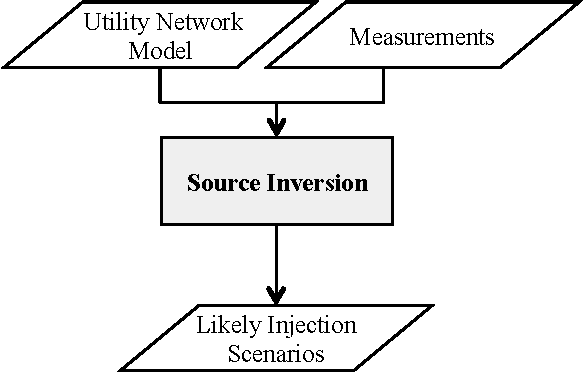
\includegraphics[scale=0.75]{graphics/inversion_flowchart.pdf}
  \caption{Contamination source identification flowchart.}
  \label{fig:inversion_command_flowchart}
\end{figure}

\section{Source Identification Formulations}\label{source_inversion_algorithms}
The \code{inversion} subcommand contains three different source identification
formulations, a Mixed Integer Programming (MIP) formulation, a
formulation based on Bayesian probability calculations and a modified
version of the Contaminant Status Algorithm by \citet{csa}. The following
subsections provide brief descriptions of these formulations. 

\subsection{MIP Formulations}
Typically, optimization based methods try to find injection candidates
that minimize the deviation between calculated values and the
measurements (e.g., least squares), penalizing any mismatch above or
below the measured values. The Mixed Integer Programming (MIP)
formulation assumes that a field sensor (or manual grab sample) would
yield a positive measurement if the contaminant concentration is above
a certain positive threshold concentration and a negative measurement
if it is below a certain negative threshold concentration. The
objective function seeks to minimize the difference between the
measured and calculated behavior according to this threshold.
%The Mixed Integer Programming (MIP) formulation assumes that a field sensor (or manual grab sample)
%would yield a positive measurement if the contaminant concentration is
%above a certain positive threshold concentration and a negative
%measurement if it is below a certain negative threshold concentration.
Therefore, if a sensor measurement (or a manual grab sample) yields a
positive measurement, any corresponding calculated concentration from
the water quality model above the positive threshold is deemed to be a
perfect fit with this measurement data. Hence, when constructing
an objective for estimation, only calculated concentrations below this
positive threshold should be minimized. Likewise, if a sensor (or
manual grab sample) yields a negative measurement, only the
corresponding calculated concentration above the negative threshold
should be minimized. Based on this idea, the base MIP formulation is presented below 
followed by descriptions of three additional variations that perform source
inversion under different assumptions. 
For more detailed information, please refer to \citet{Mann1}.


\label{sec.mip_formulation}
\begin{align}
\textrm{minimize}\qquad &\sum_{(n,t) \in \mathbf{S}_-}\mathrm{neg}_{n,t} + \sum_{(n,t) \in \mathbf{S}_+}\mathrm{pos}_{n,t} \label{eqn.milp_first_egn}\\
\textrm{subject to}\quad &Gc_{n,t} = D\mathbf{m}_R &&\forall n \in \mathbf{N}, t\in \mathbf{T} \label{eqn.milp_merlion_model}\\
&0 \le m_{n,t} \le By_n &&\forall n \in \mathbf{N},
t\in \mathbf{T} \label{eqn.milp_big_m}\\
% &m_n(t_{j-1}) \le m_n(t) &&\forall k \in \mathbf{N},
% j\in \mathbf{T}: j \neq 0 \label{eqn.mass_inj_constraint}\\
&\sum_{n \in \mathbf{N}} y_n \le I_{\max} && y_n \in \lbrace
0,1 \rbrace \label{eqn.inj_constraints}\\ &\mathrm{neg}_{n,t} \geq 0, \;\;
\mathrm{neg}_{n,t} \geq c_{n,t}-\tau _\mathrm{neg} &&\forall \left(
n,t \right) \in \mathbf{S}_- \label{eqn.milp_negative_set}\\
&\mathrm{pos}_{n,t} \geq 0, \;\; \mathrm{pos}_{n,t} \geq \tau _\mathrm{pos} -c_{n,t}
&&\forall \left(
n,t \right) \in \mathbf{S}_+. \label{eqn.milp_positive_set}
\end{align}

where $N$ is the set of all nodes, $T$ is the set of all time steps,
$S_-$ represents the set containing the node-time step pairs where the
discrete measurement is a negative detection and $S_+$ defines the set
containing the node-time step pairs where the discrete measurement is
a positive detection. The parameters $G$ and $D$ are matrices from
the Merlion water quality model. The variable $c_{n,t}$ is the
calculated concentrations from the water quality model at node $n$ and
time step $t$, $m$ is the vector of unknown time-discretized
contaminant injection profile over all node and time steps and
$m_{n,t}$ is an element in the $m_R$ vector representing unknown mass
injected at node $n$ and time step $t$. A binary variable, $y_n$,
indicates contaminant injection at node $n$ if $y_n{=}1$ and $B$ is a
reasonable upper bound on the contaminant injection mass flow rate
$m_{n,t}$. The variable $I_{\max}$ is the maximum number of possible
injection locations. The user supplies two thresholds, $\tau _\mathrm{neg}$
and $\tau _\mathrm{pos}$, which can be used as concentration set-points
indicating the presence or absence of contaminant. Having a gap
between the positive and negative threshold provides users a (buffer)
region of concentration values where really small fluctuations do not
lead to a positive measurement. Therefore, the user can specify a
higher positive threshold than the negative threshold to only flag
significant concentration changes as positive detection. The variable
$\mathrm{neg}_{n,t}$ is the non-negative difference between the modeled
concentration $c_{n,t}$ and the user supplied threshold $\tau _\mathrm{neg}$
for node-time step pairs belonging to $\mathbf{S}_-$. The variable
$\mathrm{pos}_{n,t}$ is the non-negative difference between the modeled
concentration $c_{n,t}$ and the user supplied threshold $\tau _\mathrm{pos}$
for node-time step pairs belonging to $\mathbf{S}_+$.


Equation \ref{eqn.milp_first_egn} is the MIP objective, which
minimizes the mismatch between the discrete measurements and their
corresponding concentrations calculated from the model given the
detection thresholds. Equation \ref{eqn.milp_merlion_model} is the
embedded linear water quality model (Merlion, see Section \ref{appendixMerlion} for details). 
% Note that the reduced version of this model given by equation 
% (ref) is used in place of the full model. 
Equation \ref{eqn.milp_big_m} is the big-M constraint
that enforces the bound on the maximum mass flow rate of the injections.
%\item Equation \ref{eqn.mass_inj_constraint}: Allows for the 
%case where the mass flow rate of contaminant could stay the same or increase with time.
Equation \ref{eqn.inj_constraints} is the maximum number of injections constraint, while
Equation \ref{eqn.milp_negative_set} and Equation \ref{eqn.milp_positive_set} 
are part of the reformulation of the objective function to handle the 
threshold treatment discussed above. For further details please refer to \citet{Mann1}.
They are used to 
enforce $\mathrm{neg}_{n,t}$ and $\mathrm{pos}_{n,t}$ as non-negative differences between modeled concentration and 
threshold for positive and negative measurements, $\tau _\mathrm{pos}$ and $\tau _\mathrm{neg}$, respectively. 

This base MIP formulation for
discrete measurements can be selected using the formulation option of
MIP\_discrete in the inversion block of the \code{inversion} WST
configuration file.

The source inversion problem is ill-posed with non-unique
solutions. To tackle this issue, the \code{inversion} subcommand solves
the problem multiple times, each time adding additional feasibility constraints
to exclude previously found solutions until the objective of the solution
has reduced significantly. Therefore, the final result reported by
the \code{inversion} subcommand contains a list of objective values
for each solution and the corresponding source node that was identified
for that particular solution. 

The base MIP formulation allows for any type of injection profile including the ones
shown in Figure \ref{fig:inversion_variations}. In the presence of sufficient 
measurement information, identification of any injection profile is reasonable.    
For instance, the Pulse profile in Figure \ref{fig:inversion_variations} (shown in red),
requires frequent measurements from the sensors in order to detect and characterize the injection. 
However, with relatively few fixed sensors and manual samples, identifying all
possible injection profiles can be very challenging. 
%Because of the spatial and
%temporal diversity of the possible contaminant injection profiles,
%obtaining reasonable solutions from the base formulation (in the
%presence of limited data) can be challenging. 
Therefore, in the presence of limited information, some source identification methods
only support continuous injections.   
To this aim, the \code{inversion} subcommand provides two additional restrictions that can be
applied to the base MIP formulation. 
Depending on the possible contaminant injection profile assumptions,
%additional
%restrictions can be applied to reduce the size of the search space.
Figure \ref{fig:inversion_variations} shows the different injection
profile restrictions that are supported through the different
formulation variations. The Step and No Decrease are two different 
injection profile restrictions that can be enforced by the formulation 
variations. The Pulse injection does not require additional constraints 
and is supported by the base formulation. When limited and/or less frequent measurement
data is available (e.g., only manual grab samples), the Step or the No
Decrease formulation variations are recommended.

\begin{figure}[h]
  \centering
  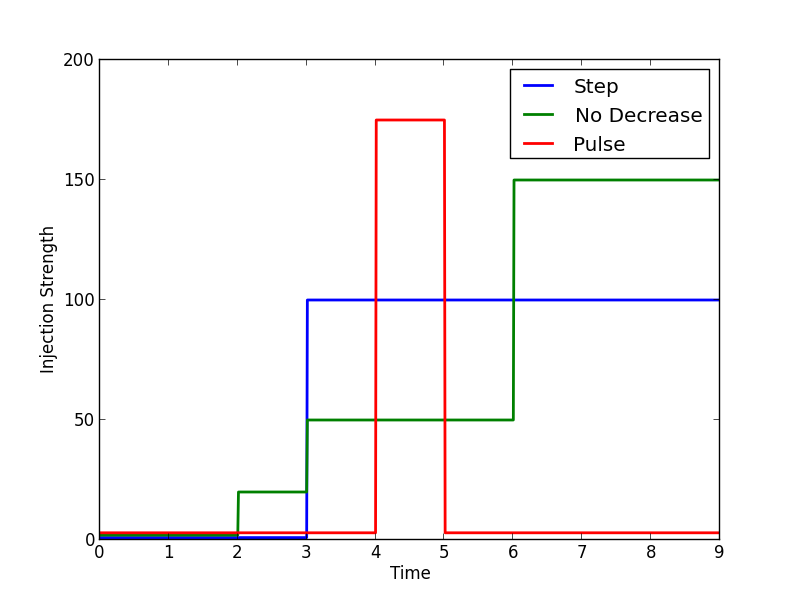
\includegraphics[scale=0.5]{graphics/inversion_injection_variation.png}
  \caption{Three different types of contamination injection profiles.}
  \label{fig:inversion_variations}

\end{figure}
             
The first variation of this formulation 
requires the injection to be a single step of any
calculated strength $S$ and can be run using the formulation option of
MIP\_discrete\_step in the inversion block. The Step profile shown in
Figure \ref{fig:inversion_variations} illustrates an example of this
type of injection. This variant is implemented by adding the following constraints to
the base formulation:

\begin{align}
&m_{n,t} \le S &&\forall n \in \mathbf{N}, t\in \mathbf{T} \\
&m_{n,t} \ge S - B(1-y_n) &&\forall n \in \mathbf{N}, t\in \mathbf{T}
\end{align}

The second variation adds constraint Equation \ref{eqn.mass_inj_constraint} 
to the base formulation to allow for
the case where the mass flow rate of the contaminant can stay the same
or increase with time. The No Decrease profile shown in
Figure \ref{fig:inversion_variations} gives an example of this kind of
injection. This variant of the formulation can be run using the
formulation option of MIP\_discrete\_nd in the inversion block.

\begin{align}
 &m_{n,t-1} \le m_{n,t} &&\forall n \in \mathbf{N}, t\in \mathbf{T}:
 j \neq 0 \label{eqn.mass_inj_constraint}
\end{align}

The third variation solves the Step formulation by fixing the binary
variable $y_n$ corresponding to a source node and solving the
resulting linear program (LP) for all nodes $n \in, N$. The objective
values for all LP solutions are compared and only a fraction of the
identified nodes are reported in the results based on
the candidate threshold option in inversion block of the configuration file. 
This LP variant can be run using the formulation option of
LP\_discrete in the inversion block.

\subsection{Bayesian Probability Based Formulation}
\label{sec.bayesian_algorithm}
This formulation calculates the probability of a node being the true
injection node using Bayes rule:
\begin{align}
P(i|m) = \frac{P(m|i)P(i)}{P(m)} \label{source_probability}
\end{align}
where contamination incident $i$ is an injection at a node and at a particular time step and $P(i|m)$ is 
the probability of an incident $i$ given a set of measurements $m$. Here, $P(i)$ is the 
prior probability of an incident. This formulation assumes that only a single injection 
incident is possible, and therefore it uses an uniform prior of 1/(all possible incidents). 
Since it is difficult to estimate $P(m)$ (the prior probability of a measurement), 
this calculation is substituted by obtaining the $P(i|m)$ for all possible incidents and 
then normalizing them to 1. Finally, $P(m|i)$ is the probability of a measurement 
given an injection incident. It is calculated using the following equation:


\begin{align}
P(m|i) = (1-p_f)^{\mathrm{match}(i)}p_f^{\mathrm{meas} - \mathrm{match}(i)}
\end{align}
where, $p_f$ is the probability of measurement failure, $\mathrm{meas}$ is the total number 
of measurements and $\mathrm{match}(i)$ is the number of discrete measurements that match the discrete concentrations 
obtained by simulating incident $i$. Note that calculating the discrete concentration profile 
obtained by simulating an incident requires a threshold that is specified by using the negative threshold option of the inversion block of the 
\code{inversion} configuration file.

After calculating the normalized probability $P(i|m)$ for all
incidents, only those having a probability above a confidence limit
are reported as the set of likely incidents along with their
corresponding $P(i|m)$ values. This
confidence limit is by default set to 95\% (0.95) and can be changed
by using the confidence option of the inversion block.

\subsection{Contaminant Status Algorithm (CSA)}
\label{sec.csa_algorithm}

The Contaminant Status Algorithm (CSA), proposed by \citet{csa},
performs source identification by assigning a status to each candidate
node-time pair as either being safe (not an injection candidate),
unsafe (possible injection candidate) or unknown. In WST, the CSA has
been modified to assign a likeliness measure of 1 to a node if it is
contained in the list of unsafe node-time pairs, while all other nodes
are assigned a likeliness measure of 0.

CSA uses a linear input-output water quality model generated through
the Particle Backtracking Approach (PBA) proposed
by \citet{Shang2002}. For every sensor $j$ and analysis time $t$, this
model provides the upstream reachability set, $U_j(t)$, that contains
the list of node-time pairs that are hydraulically connected to that
measurement. Using this set, a station source matrix, $S_j$, which
represents the list of safe, unsafe and unknown nodes based on all the
measurements available from sensor node $j$ only, is updated
iteratively using the following algorithm:

\begin{enumerate}
\item Initialize $S_j(i,\hat{t}) = $ Unknown, $\forall i \in \mathbf{N}, \forall \hat{t} \in \mathbf{T} $
\item For $(i,\hat{t}) \in U_j(t)$
        \begin{enumerate}
                \item For significant hydraulic connections (based on a threshold in the PBA input-output model)-
                        if the current measurement at sensor $j$ is positive, Set $S_j(i,\hat{t}) = $ Unsafe,
                        else Set $S_j(i,\hat{t}) = $ Safe
                \item For weak hydraulic connections (based on a threshold in the PBA input-output model), Set $S_j(i,\hat{t}) = $ Unknown
        \end{enumerate}
\end{enumerate}
where $N$ is the set of all candidate nodes and $T$ is the set of all
time steps in the time horizon. Based on the status from every
station source matrix, $S_j$, a total source status matrix $S$ that
contains the overall status of all candidate node-time pairs,
$(i,\hat{t})$, is updated using the following rules - an unsafe
node-time pair can only change to safe based on its corresponding
state in $S_j$; an unknown node-time pair can change to both safe or
unsafe; and if a node-time pair is safe, it will remain safe. Hence,
the total source status matrix is also updated iteratively over the
complete list of measurement time steps to obtain the final status of
all candidate injection node-time pairs. Consequently, CSA allows for
multiple simultaneous injections, however, it assumes perfect
measurements when marking candidate injections as safe.


\section{Source Identification Solvers}

The MIP algorithm builds an optimization formulation, and requires a MIP 
solver to perform source inversion. Therefore, if the MIP algorithm is selected 
(\code{algorithm:\ optimization}) as described in Section 
\ref{sec.inversion_subcommand.config_options}), then a solver needs to be 
specified. The solvers recognized by the \code{inversion} subcommand are 
the same as those recognized by \code{booster\_mip} subcommand (See 
Section \ref{booster_mip_solver} for more details).

\section{\code{inversion} Subcommand}\label{sec.inversion_subcommand}

The \code{inversion} subcommand is executed using the following
command line:
\begin{unknownListing}
wst inversion <configfile>
\end{unknownListing}
where \code{configfile} is a WST configuration file in the YAML format.

The \code{---help} option prints information about this subcommand,
such as usage, arguments and a brief description:
\begin{unknownListing}
wst inversion --help
\end{unknownListing}

\subsection{Configuration File}

The \code{inversion} subcommand generates a template configuration
file using the following command line:

\begin{unknownListing}
wst inversion --template <configfile>
\end{unknownListing}

The \code{inversion} template configuration file is shown in
Figure \ref{fig:inversion_template}. Brief descriptions of the
options are included in the template after the \# sign.

\begin{figure}[!ht]
  \unknownInputListing{examples/inversion_config.yml}{}{1}{35}
  \caption{The \code{inversion} configuration template file.}
  \label{fig:inversion_template}
\end{figure}

\subsection{Configuration Options}\label{sec.inversion_subcommand.config_options}

Full descriptions of the WST configuration options used by the \code{inversion} subcommand are listed below.
\begin{description}[topsep=0pt,parsep=0.5em,itemsep=-0.4em]
  \item[{network}]\hfill
  \begin{description}[topsep=0pt,parsep=0.5em,itemsep=-0.4em]
    \item[{epanet file}]\hfill
\\ The name of the EPANET 2.00.12 input (INP) file that defines the water distribution
                network model.
                
                Required input.
  \end{description}
  \item[{measurements}]\hfill
  \begin{description}[topsep=0pt,parsep=0.5em,itemsep=-0.4em]
    \item[{grab samples}]\hfill
\\The name of the file that contains all the measurements from 
                the manual grab samples and the fixed sensors. The measurement file 
                format is documented in File Formats Section \ref{formats_measFile}.

                Required input.
  \end{description}
  \item[{inversion}]\hfill
  \begin{description}[topsep=0pt,parsep=0.5em,itemsep=-0.4em]
    \item[{algorithm}]\hfill
\\The algorithm used to perform source inversion. The options are 
				optimization, bayesian, or csa. The optimization algorithm requires 
				AMPL or PYOMO along with a MIP solver. The bayesian algorithm 
				uses Bayes' Rule to update probability of a particular node 
				being the contaminant source node. The CSA is the Contaminant
                                Status Algorithm by \citet{csa}.
                
                Required input, default = optimization.
    \item[{formulation}]\hfill
\\The formulation used by the optimization algorithm. The options are 
                LP\_discrete (discrete LP), MIP\_discrete (discrete MIP), 
                MIP\_discrete\_nd (discrete MIP with no decrease) or 
                MIP\_discrete\_step (discrete MIP for step injection).
                
                Required input for optimization algorithm, default = MIP\_discrete.
    \item[{model format}]\hfill
\\The modeling language used to build the formulation specified
                by the formulation option. The options are AMPL and PYOMO. 
				AMPL is a third party package that must be installed by 
				the user if this option is specified. PYOMO is an open source 
				software package that is distributed with WST.
                
                Required input for optimization algorithm, default = PYOMO.
    \item[{merlion water quality model}]\hfill
\\This option is set to true to use the Merlion 
                water quality model for simulating the candidate injections
                in the Bayesian probability-based method. It can be set to false
                to use EPANET 2.00.12 for these simulations. Note that the Merlion water quality
                model is required in either case to generate the initial list of candidate injections.
 
                Optional input, default = true.
    \item[{horizon}]\hfill
\\The minutes over which the past measurement
                data is used for source inversion. It is calculated backwards from
                the latest measurement time in the measurements file. 
                All measurements in the measurements file that are within the horizon 
                are used (both negative and positive). In the case of the CSA algorithm, 
                the implementation assumes fixed sensors only, and all measurements at 
                these sensors are assumed to be negative prior to the horizon.
                If the horizon is longer
                than the time between the latest measurement and simulation start time,
                then all the measurements are used for source inversion.
                
                Required input, default = None (Start of simulation).
    \item[{num injections}]\hfill
\\The number of possible injections to consider when
                performing inversion. Multiple injections are only supported by
                the MIP formulation. This value must be set to 1 for the LP model
                or the probability algorithm.
                
                Required input for optimization algorithm, default = 1.
    \item[{measurement failure}]\hfill
\\The probability that a sensors gives an incorrect reading. Must be between 0 and 1. 
                
                Required input for the Bayesian algorithm, default = 0.05.
    \item[{positive threshold}]\hfill
\\The concentration threshold used by the sensors to flag a positive 
                detection measurement. This is a parameter in the optimization algorithm (Equation \ref{eqn.milp_positive_set}).
                
                Required input for optimization algorithm, default = 100 mg/L. 
    \item[{negative threshold}]\hfill
\\The concentration threshold used by the sensors to flag
                a negative detection measurement. This is a parameter in the
                optimization algorithm (Equation \ref{eqn.milp_negative_set}).
                
                Required input for optimization algorithm, default = 0.0 mg/L.
    \item[{feasible nodes}]\hfill
\\A list that defines nodes that can be considered for the source inversion problem.
                The options are: (1) ALL, which specifies all nodes as feasible source locations;
                (2) NZD, which specifies all non-zero demand nodes as feasible source locations;
                (3) a list of EPANET node IDs, which identifies specific nodes as feasible source locations; or
                (4) a filename, which is a space or comma separated file containing a list of 
                specific nodes as feasible source locations. 

                Optional input.
    \item[{candidate threshold}]\hfill
\\The objective cut-off value for candidate contamination incidents 
                using the optimization algorithm. The objective value represents the
                likelihood of a particular node being the injection node (See Equation \ref{eq_transform_obj}).  
                The objective values are normalized to 1 and only the nodes having 
                their objective values greater or equal to the threshold are reported
                in the inversion results. 
                
                Required input for optimization algorithm, default = 0.20.
    \item[{confidence}]\hfill
\\The probability cut-off value for candidate contamination incidents
                using the Bayesian algorithm. The value is between 0 and 1. 
                
                Required for the Bayesian algorithm, default = 0.95.
    \item[{output impact nodes}]\hfill
\\A option to output a Likely\_Nodes.dat file that contains only
                the node IDs of the possible contaminant injection nodes obtained from the 
                \code{inversion} subcommand. This file can be used as the feasible nodes for the next 
                iteration of the \code{inversion} subcommand to only consider this set of possible contaminant 
                injection nodes.
                
                Optional input, default = false.
  \end{description}
  \item[{solver}]\hfill
  \begin{description}[topsep=0pt,parsep=0.5em,itemsep=-0.4em]
    \item[{type}]\hfill
\\The solver type. Each component of WST
				(e.g., sensor placement, flushing response, booster 
				placement) has different 
				solvers available. More specific details are provided in 
				the subcommand's chapter.
                
                Required input.
    \item[{options}]\hfill
\\A list of options associated with a specific solver type. More
            information on the options available for a specific solver
            is provided in the solver's documentation. The Getting
            Started Section \ref{dependencies} provides links to the
            different solvers.
            
            Optional input.
    \item[{threads}]\hfill
\\The maximum number of threads or function evaluations the solver is
                allowed to use.  This option is not available to all solvers or all analyses.
                
                Optional input.
    \item[{logfile}]\hfill
\\The name of a file to output the results of the solver.
                
                Optional input.
    \item[{verbose}]\hfill
\\The solver verbosity level.
                
                Optional input, default = 0 (lowest level).
    \item[{initial points}]\hfill
    \begin{description}[topsep=0pt,parsep=0.5em,itemsep=-0.4em]
      \item[{nodes}]\hfill
\\A list of node locations (EPANET IDs) to begin the optimization
        process. Currently, this option is only supported for the
        network solver used in the flushing and booster\_msx
        subcommands. This input causes an error for other subcommands.
        
        Optional input.
      \item[{pipes}]\hfill
\\A list of pipe locations (EPANET IDs) to begin the optimization
        process. Currently, this option is only supported for the
        network solver used in the flushing subcommand. This input causes an error for other subcommands.
        
        Optional input.
    \end{description}
  \end{description}
  \item[{configure}]\hfill
  \begin{description}[topsep=0pt,parsep=0.5em,itemsep=-0.4em]
    \item[{output prefix}]\hfill
\\The prefix used for all output files.
                
                Required input.
    \item[{output directory}]\hfill
      \\The output directory to store the results.
    \item[{debug}]\hfill
\\The debugging level (0 or 1) that indicates the amount of debugging 
                information printed to the screen, log file and output yml file. 
                
                Optional input, default = 0 (lowest level).
  \end{description}
\end{description}


\subsection{Subcommand Output}
% The <output prefix>inversion.json file contains a summary of 
% the \code{inversion} subcommand results. This file includes a list of
% node locations along with their objective or probability values, in 
% which a higher value indicates a higher likelihood of that node being 
% the true contaminant injection node.  The injection profiles (start 
% and end times and the strength) for each possible injection node are 
% also included along with the run date and CPU time for inversion.
% The \code{inversion} subcommand also outputs an 
% <output prefix>profiles.tsg file that contains the list of likely 
% injection profiles in the TSG file format (See File Formats 
% Section \ref{formats_tsgFile}). As discussed in Chapter \ref{chap:grabsample}, this TSG
% file can be directly used as an input by the \code{grabsample} 
% subcommand.

The \code{inversion} subcommand creates several output files. 
The YAML file called <output prefix>inversion\_output.yml 
contains a list of possible source node locations (EPANET node IDs),  
the associated objective or probability value (node likeliness) for each possible source node 
(a higher value indicates a higher likelihood of that node being 
the true contaminant injection node), the injection profiles (start 
and end times and the strength) for each possible source node, 
the run date and CPU time. 
The log file called <output prefix>inversion\_output.log contains basic debugging information. 
The \code{inversion} subcommand also outputs an 
<output prefix>\_profile.tsg file that contains the list of likely 
injection profiles in the TSG file format (See File Formats 
Section \ref{formats_tsgFile}). As discussed in Chapter \ref{chap:grabsample}, this TSG
file can be directly used as an input by the \code{grabsample} 
subcommand.
A visualization YAML configuration file named <output prefix>inversion\_output\_vis.yml is also created.
The \code{visualization} subcommand is automatically run using this YAML file.

\section{Source Identification Examples}
Three examples illustrating the use of the different source identification
methods available in WST are presented. In the first example, the optimization
formulation is used to solve a source identification problem, while the
second example uses the Bayesian probability formulation and the third example 
uses the Contaminant Status Algorithm (CSA) to solve the exact same problem. 
An EPANET 2.00.12 network model (INP format) and a measurements file (See File
Formats Section \ref{formats_measFile}) are required to run
the \code{inversion} subcommand. 

Since real system data is not available, a measurements file required for
the \code{inversion} subcommand can be generated using
the \code{measuregen} executable (Executable Files Section \ref{measuregenExecutable}). 
The three examples use the EPANET Example Network 3 input file (Net3.inp) 
as the network file, which runs a two day hydraulic and water
quality simulation. An injection at node 151 is simulated 
from 8 hours until 24 hours, specified using
the Net3\_inversion.tsg file. The sensor locations are provided using
the Net3\_fixed\_sensors file, and the measurements are obtained every
15 minutes with a concentration threshold of 0 indicating
contamination. The following command line statement can be run from
the examples folder to generate the measurements file:

\begin{unknownListing}
measuregen --inp=Net3/Net3.inp --tsg=Net3/Net3_inversion.tsg --start-sensing-time=0 
--stop-sensing-time=705 --measures-per-hour=4 --threshold=0 --ignore-merlion-warnings 
--output-prefix=Net3/Net3 Net3/Net3_fixed_sensors
\end{unknownListing}

The resulting Net3\_MEASURES.dat file is used in the following three examples. 

\subsection{Example 1}  
In the first example, the optimization method is used to solve 
the source identification problem. The configuration file, 
inversion\_ex1.yml, shown in Figure \ref{fig:inversion_ex1} is used to
identify the possible contaminant source locations. The MIP
optimization formulation, MIP\_discrete\_step, is used for this
example. The example uses the Net3\_MEASURES.dat file
generated using the \code{measuregen} executable.

\begin{figure}[!ht]
  \unknownInputListing{../../examples/inversion_ex1.yml}{}{1}{26}
  \caption{The \code{inversion} configuration file for example 1.}
  \label{fig:inversion_ex1}
\end{figure}

The example can be executed using the following command line:
\begin{unknownListing}
wst inversion inversion_ex1.yml
\end{unknownListing}

The results are contained in the file {\outputprefix}inversion\_output.yml.
A section of this results file is shown in
Figure \ref{fig:inversion_ex1_re}. The results contain a list of sets
where each set contains - possible contaminant source node in the
Nodes list (which contains a node Name and a Profile), CPU
computation time in seconds and the Objective value corresponding
to the solution which identifies that node as the source node. The
Objective value for each candidate node $n$ in the results file is
related to the objective of the MIP
formulations \ref{sec.mip_formulation}
(Equation \ref{eqn.milp_first_egn}). The objective calculated from the
MIP formulation is transformed such that it is normalized to 1 and a
higher value means a higher likelihood of a node being the source
node. This transformation is done by the following equations:
\begin{align}
\textrm{INV\_NORM\_OBJ}_n &= 1 - \frac{\textrm{FORM\_OBJ}_n}{\max(\textrm{FORM\_OBJ})} &&\forall n \in \mathbf{N}\\
\textrm{Objective}_n &= \frac{\textrm{INV\_NORM\_OBJ}_n}{\max(\textrm{INV\_NORM\_OBJ})} &&\forall n \in \mathbf{N} \label{eq_transform_obj}
\end{align}
where $\textrm{FORM\_OBJ}_n$ (Formulation Objective) is the objective
value as calculated from the MIP formulation
Equation \ref{eqn.milp_first_egn} when node $n$ is identified as the
most likely node, $\textrm{INV\_NORM\_OBJ}_n$ is an intermediate
variable that represents one (1) minus the normalized formulation objective
and $\textrm{Objective}_n$ is the normalized form of the
$\textrm{INV\_NORM\_OBJ}_n$ which is reported in the \code{inversion}
subcommand results file.
   
This results file only contains the list
of possible contaminant source nodes that have an objective (as calculated by \ref{eq_transform_obj}) greater
than the candidate threshold provided in the inversion block of the WST configuration
file. 

\begin{figure}[!ht]
  \unknownInputListing{examples/inversion/inversion_ex1_output.yml}{}{1}{15}
  \caption{The \code{inversion} YAML output file for example 1.}
  \label{fig:inversion_ex1_re}
\end{figure}

For this example scenario, the \code{inversion} subcommand is able to
correctly identify node 151 as one of the three most likely source
nodes. This means that given the current measurement information
available, nodes 151, 153 and 149 are equally likely. Further
measurements can be obtained from selected grab sampling locations that
can help in distinguishing between these three potential source
nodes. 
An example of how to use the \code{grabsample} subcommand to
optimally select grab sampling location to improve the identification of the 
true contamination source is provided in the source identification case study 
in the Advanced Topics and Case Studies chapter \ref{inversion_case_study}.

\subsection{Example 2}  
In this example, the Bayesian probability formulation is used to solve
the same problem described in example 1. The configuration file,
inversion\_ex2.yml, shown in Figure \ref{fig:inversion_ex2}, is used for
this example. The bayesian formulation is selected
by using the algorithm option in the inversion
block.
 
\begin{figure}[!ht]
  \unknownInputListing{../../examples/inversion_ex2.yml}{}{1}{26}
  \caption{The \code{inversion} configuration file for example 2.}
  \label{fig:inversion_ex2}
\end{figure}


The example can be executed using the following command line:
\begin{unknownListing}
wst inversion inversion_ex2.yml
\end{unknownListing}

The results are contained in the file {\outputprefix}inversion\_output.yml
shown in Figure \ref{fig:inversion_ex2_re}. The likeliness value
reported in this file corresponds to the probability value calculated
by Equation \ref{source_probability}. The probability algorithm is
also able to correctly identify node 151 as the one of the three most
probable source nodes along with nodes 149 and 153. 

\begin{figure}[!ht]
  \unknownInputListing{examples/inversion/inversion_ex2_output.yml}{}{1}{13}
  \caption{The \code{inversion} YAML output file for example 2.}
  \label{fig:inversion_ex2_re}
\end{figure}

\subsection{Example 3}  
In this example, the Contaminant Status Algorithm (CSA) is used to solve
the same problem described in example 1. The configuration file,
inversion\_ex3.yml, shown in Figure \ref{fig:inversion_ex3}, is used for
this example. CSA is selected
by using the algorithm option in the inversion
block.
 
\begin{figure}[!ht]
  \unknownInputListing{../../examples/inversion_ex3.yml}{}{1}{26}
  \caption{The \code{inversion} configuration file for example 3.}
  \label{fig:inversion_ex3}
\end{figure}


The example can be executed using the following command line:
\begin{unknownListing}
wst inversion inversion_ex3.yml
\end{unknownListing}

The results are contained in the file
{\outputprefix}inversion\_output.yml shown in
Figure \ref{fig:inversion_ex3_re}. Since in WST, a
likeliness measure of 1 is assigned to a node if it is contained in the list of
unsafe node-time pairs, while a likeliness measure of 0 is assigned to all other nodes, 
the node likeliness in the results output file is 1.0 for all possible contamination injection nodes. 
CSA is also able to correctly identify node 151 as the one of the four most probable
source nodes along with nodes 125, 149 and 153.

\begin{figure}[!ht]
  \unknownInputListing{examples/inversion/inversion_ex3_output.yml}{}{1}{13}
  \caption{The \code{inversion} YAML output file for example 3.}
  \label{fig:inversion_ex3_re}
\end{figure}



  
  \chapter{Uncertainty Quantification}
  \label{chap:uq}
  Mathematical models used to simulate water distribution systems are subject to uncertainty. 
Effective characterization of uncertainty is critical for reliable analysis with simulation-based studies. 
Particularly for contamination incidents, uncertainty quantification is needed to effectively 
use simulation tools that provide insights into response actions. 
Hydraulic parameters that might cause uncertainty include: 
(1) customer demands at each node and time, (2) operational controls (e.g., valve settings, pump curves), (3) 
infrastructure topography and characteristics (e.g., missing pipes or junctions, effective pipe diameters) and (4) initial conditions (e.g., tank levels, pump statuses). 
Water quality parameters that might cause uncertainty include: 
(1)  initial water quality, (2) contaminant species, (3) contaminant reaction dynamics, (4) the amount
of contaminant injected, (5) injection location, (6) injection time and (7) injection duration.

The \code{uq} subcommand examines the effect of hydraulic and water quality uncertainty on the extent of contamination in terms of the identification of the contamination source. 
This subcommand can be used to quantify uncertainty after running source identification using the Bayesian probability based formulation (Section \ref{sec.bayesian_algorithm}). Given a particular confidence level, nodes can be categorized according to their probability of contamination. Nodes whose contamination probability, $\gamma_n$, that are above a 
threshold are labeled with respect to their contamination state as LY for ``likely yes,'' LN for``likely no'' and UN for ``unknown.''  
For example, for a 95\% confidence level: 

\[ \left\{ \begin{array}{ll}
         \gamma_n \geq 0.975 & \mbox{LY},\\
        0.025\leq \gamma_n \leq 0.975 & \mbox{UN}, \\
        \gamma_n \leq 0.025 & \mbox{LN} \end{array} \right. 
\] 

With the \code{uq} subcommand 
the effects of uncertainty in customer demand, isolation valve status, bulk reaction rate coefficient and 
contaminant injection location, start time, duration and rate can be studied on the size and location of the contamination incident.

A flowchart representation of the \code{uq} subcommand is shown in Figure \ref{fig:uq_flowchart}. Given a list of EPANET 2.00.12 compatible network models (INP format) 
coupled with a list of injection scenarios (TSG format), the \code{uq} subcommand
runs Monte Carlo simulations to estimate the probability that each node in the network is contaminated.

\begin{figure}[h]
	\centering
	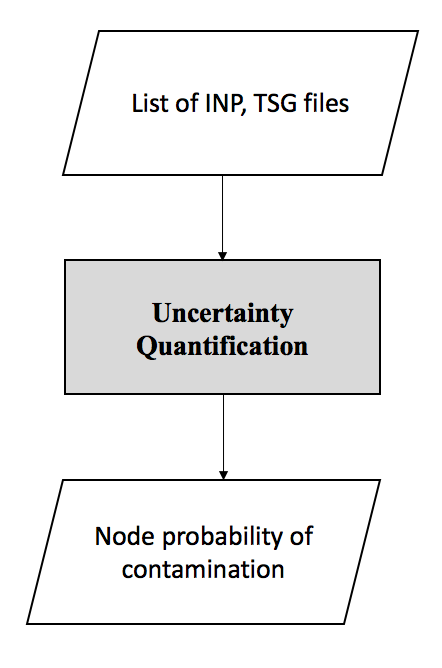
\includegraphics[scale=0.30]{graphics/uq_flowchart.png}
	\caption{Uncertainty quantification flowchart.}
	\label{fig:uq_flowchart}
\end{figure}

\section{Uncertainty Quantification Method}\label{uqn_algorithms}
The \code{uq} subcommand runs an ensemble of scenarios where each scenario is defined using an INP and TSG file. The INP and TSG files 
contain the hydraulic and water quality parameters for the scenario.  
The results are used to compute the probability that each node is contaminated, using the following equation:
\begin{equation}
\gamma_n = \sum_{s \in S} \delta_{s,n}\beta_s
\label{nodeprob}
\end{equation}
where $\gamma_n $ is the probability that node $n$ is contaminated, $\beta_s$ is the probability of scenario $s$ and $\delta_{s,n}$ is a binary parameter that is $1$ if scenario $s$ contaminates node $n$, and $0$ otherwise. The values of $\delta_{s,n}$ are determined from the simulations over the full potential scenario set, and the values for $\beta_s$ are determined using equation~\eqref{source_probability} based on previous measurements provided in the measurements file. If no measurements file is provided, then the values for $\beta_s$ are assumed to be uniform. A threshold value is used to decide whether a node is contaminated or not in a single scenario.

\section{\code{uq} Subcommand}\label{sec.uq_subcommand}

The \code{uq} subcommand is executed using the following command line:
\begin{unknownListing}
wst uq <configfile>
\end{unknownListing}
where \code{configfile} is a WST configuration file in the YAML format.

The \code{---help} option prints information about this subcommand,
such as usage, arguments and a brief description:
\begin{unknownListing}
wst uq --help
\end{unknownListing}

\subsection{Configuration File}

The \code{uq} subcommand generates a template configuration
file using the following command line:

\begin{unknownListing}
wst uq --template <configfile>
\end{unknownListing}

The \code{uq} template configuration file is shown in
Figure \ref{fig:uq_template}. Brief descriptions of the
options are included in the template after the \# sign.

\begin{figure}[h]
  \unknownInputListing{examples/uq_config.yml}{}{1}{17}
  \caption{The \code{uq} configuration template file.}
  \label{fig:uq_template}
\end{figure}

\subsection{Configuration Options}\label{sec.uq_subcommand.config_options}

Full descriptions of the WST configuration options used by the \code{uq} subcommand are listed below.
\begin{description}[topsep=0pt,parsep=0.5em,itemsep=-0.4em]
  \item[{scenario}]\hfill
  \begin{description}[topsep=0pt,parsep=0.5em,itemsep=-0.4em]
    \item[{signals}]\hfill
\\Name of file or directory with information to generate 
                or load signals. If a file is provided the list of inp tsg tuples
                 will be simulated and the information stored in signals files. If
                a directory with the signals files is specified, the signal files will
                be read and loaded in memory. This input is only valid for the uq
                subcommand and the grabsample subcommand with probability based formulations.

                Required input.
  \end{description}
  \item[{uq}]\hfill
  \begin{description}[topsep=0pt,parsep=0.5em,itemsep=-0.4em]
    \item[{analysis time}]\hfill
\\The time at which the manual grab sample should be taken. 
                The algorithm determines the best possible manual grab sample location(s)
                based upon this time. Units: Minutes from the simulation start time in the
                EPANET 2.00.12 INP file.
    \item[{threshold}]\hfill
      \\This threshold determines whether or not an incident impacts a
      location (mg/L).
    \item[{filter scenarios}]\hfill
\\ This options enables filtering scenarios. Only those scenarios 
                that match at least one of the measurements are considered
                in the optimal sampling analysis, default = False.
    \item[{measurement failure}]\hfill
\\The probability that a sensor gives an incorrect reading. Must be between 0 and 1. 
                
                Required input for the Bayesian algorithm, default = 0.05.
    \item[{confidence}]\hfill
\\The probability cut-off value for classifying nodes as certain to be contaminated, 
                uncertain to be contaminated and certain to not be contaminated. The value is 
                between 0 and 1. Nodes with probability greater than (((1-confidence)/2)+confidence) are 
                classified likely to be contaminated or likely yes LY, 
                nodes with probability less than ((1-confidence)/2) are classified likely not contaminated
                LN and nodes with probability in between are uncertain nodes UN.
                
                Required for node classification, default = 0.95 (unitless).
  \end{description}
  \item[{measurements}]\hfill
  \begin{description}[topsep=0pt,parsep=0.5em,itemsep=-0.4em]
    \item[{grab samples}]\hfill
\\The name of the file that contains all the measurements from 
                the manual grab samples and the fixed sensors. The measurement file 
                format is documented in File Formats Section \ref{formats_measFile}.

                Optional input.
  \end{description}
  \item[{configure}]\hfill
  \begin{description}[topsep=0pt,parsep=0.5em,itemsep=-0.4em]
    \item[{output prefix}]\hfill
\\The prefix used for all output files.
                
                Required input.
    \item[{output directory}]\hfill
      \\The output directory to store the results.
    \item[{debug}]\hfill
\\The debugging level (0 or 1) that indicates the amount of debugging 
                information printed to the screen, log file and output yml file. 
                
                Optional input, default = 0 (lowest level).
  \end{description}
\end{description}


\subsection{Subcommand Output}
The \code{uq} subcommand creates two YAML files called <output prefix>\_uq\_scenarios.yml and <output prefix>\_uq\_nodes.yml that contain
a list of probabilities for the scenarios and nodes, respectively.
The log file named <output prefix>uq\_output.log contains basic debugging information. 

\section{Uncertainty Quantification Example}

A list of EPANET 2.00.12 INP and TSG files are required to run the \code{uq} subcommand. The configuration file for this example, uq\_ex1.yml, is shown in Figure \ref{fig:uq_confex1}. 

\begin{figure}[h]
  \unknownInputListing{../../examples/uq_ex1.yml}{}{1}{17}
  \caption{The \code{uq} configuration file for example 1.}
  \label{fig:uq_confex1}
\end{figure}

The file with the list of scenarios for this example is shown in Figure \ref{fig:uq_scenarios}.

\begin{figure}[h]
  \unknownInputListing{../../examples/Net3/uq/list_scenarios.dat}{}{1}{3}
  \caption{List of scenarios.}
  \label{fig:uq_scenarios}
\end{figure}

Summary information is printed to the screen, as shown in Figure \ref{fig:uq_out1}.

\begin{figure}[h]
  \unknownInputListing{examples/uq/uq_ex1_screen_output.txt}{}{1}{31}
  \caption{Screen output for example 1.}
  \label{fig:uq_out1}
\end{figure}

The results from the \code{uq} subcommand can be represented in probability maps using the \code{visualization} subcommand (Chapter 11). 


  \chapter{Grab Sampling}
  \label{chap:grabsample}
  When source identification is performed following initial detection of a
contamination incident, it is likely that the identified set of
possible injection locations is fairly large due to the limited
measurement information available at the early stages of detection.
As time progresses, more measurements become available to help
decrease the number of possible injection locations. It is possible to
obtain additional measurements in the form of grab samples from
optimally selected locations that can help in quickly narrowing down
the set of likely incident locations when source inversion
calculations are performed again. The \code{grabsample} subcommand can be used to
identify optimal grab sample locations 
that are likely to provide the most information in narrowing down the 
list of possible injection locations identified from
the \code{inversion} subcommand.

A flowchart representation of the \code{grabsample} subcommand is
shown in Figure \ref{fig:grabsample_flowchart}. The required input
for the \code{grabsample} subcommand includes a utility network model
specified with an EPANET 2.00.12 compatible input file (INP) and a list of
likely injection scenarios.
%A flowchart representation of the \code{grabsample} subcommand, used in conjunction with the 
%\code{inversion} subcommand, is shown in Figure \ref{fig:inversion_grabsample_flowchart}. 


\begin{figure}[h]
  \centering
  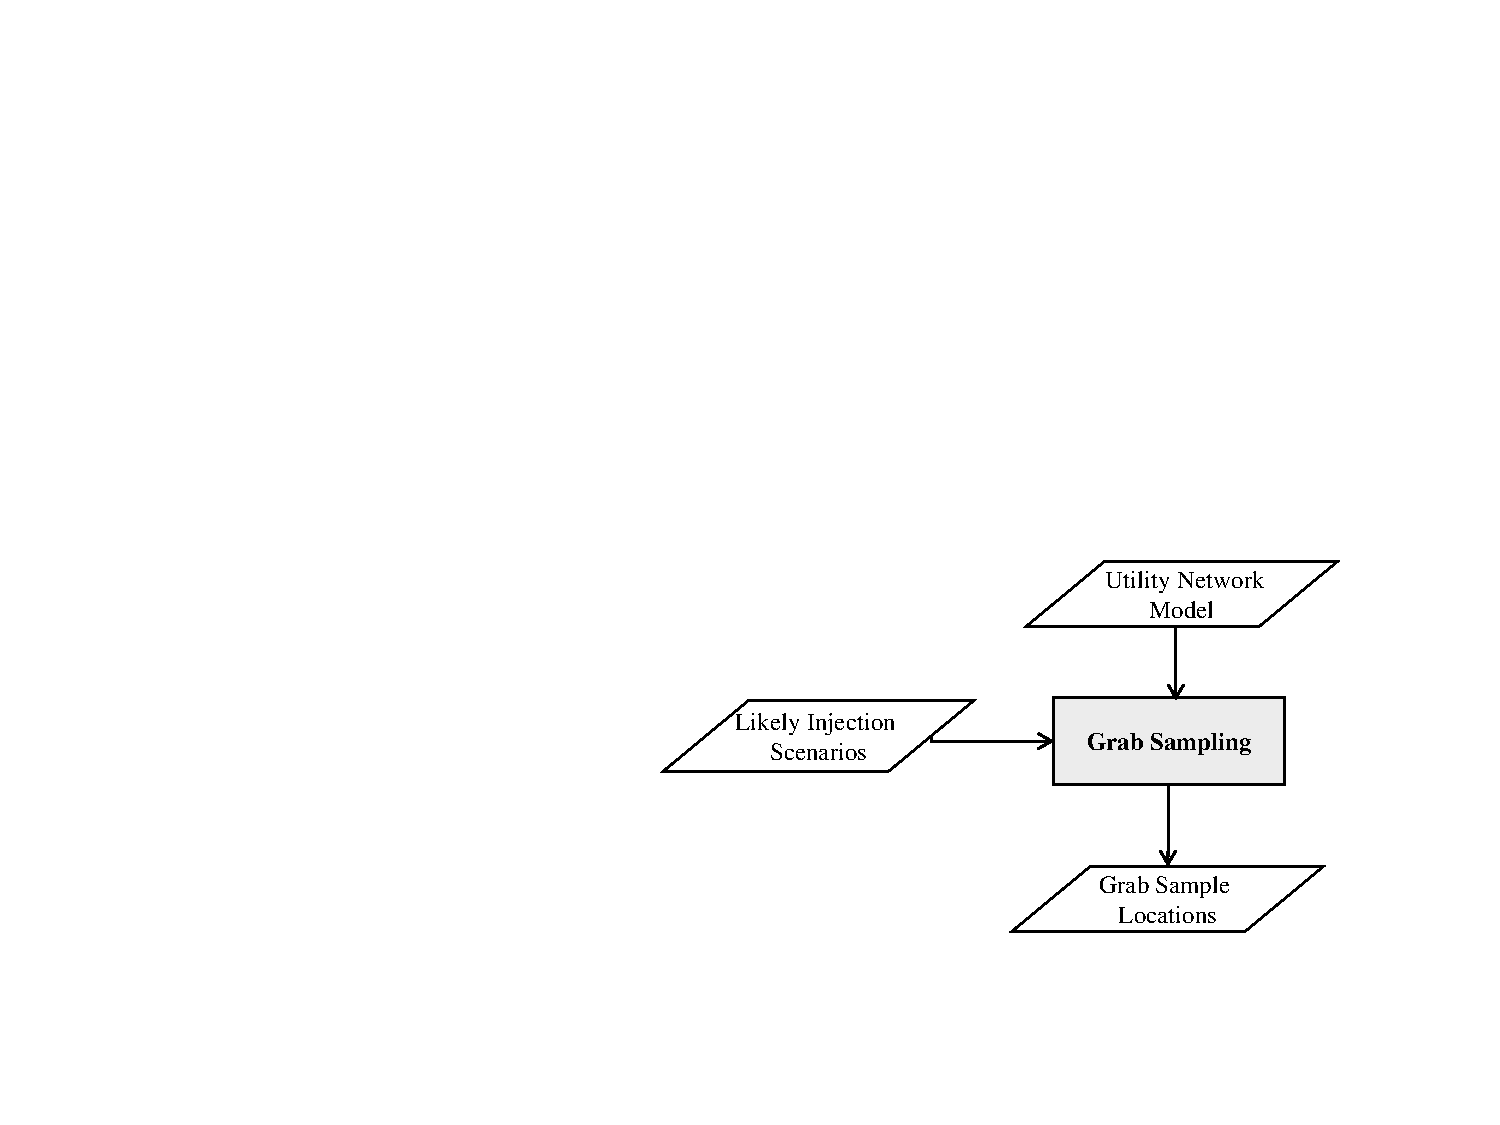
\includegraphics[scale=0.75]{graphics/grabsample_flowchart.pdf}
  \caption{Grab sample flowchart.}
  \label{fig:grabsample_flowchart}
\end{figure}

\section{Grab Sample Formulations}
The \code{grabsample} subcommand contains three different grab sampling formulations, 
the distinguishability formulation and two probability-based formulations.
The probability functions will likely be faster for larger problems (linear scaling), while the distinguishability formulation scales quadratically with the number of contamination scenarios. 
The following subsections provide brief descriptions of these formulations.

\subsection{Distinguishability Formulation}
\label{grabsample_formulation}
Considering two possible contamination incidents $i$ and $j$, if a
particular sample location is impacted by incident $i$, but not
impacted by incident $j$, then this sample location is able to
distinguish between the two incidents. The \code{grabsample} subcommand
can be used to identify grab sample locations that maximize the number
of pairwise distinguishable incidents in a list of possible
contamination incidents. The <output prefix>profile.tsg obtained
from the \code{inversion} subcommand contains a list of possible injection
locations. The data sets required by the optimization formulation
below are obtained by simulating each possible incident using the
EPANET 2.00.12 hydraulics model and either the EPANET 2.00.12 water quality model or the Merlion water quality model \citep{Mann1},
which can be selected using the merlion option in the scenario block of the configuration file.

The distinguishability problem formulation is:
\begin{align}
\textrm{maximize}\qquad &\sum_{(i,j) \in PE} d_{ij}\label{eqn.grabsample_obj}\\
\textrm{subject to} \qquad &\sum_{n \in D_{ij}}s_n \geq d_{ij} &&\forall \left( i,j \right) \in PE \label{eqn.grabsample_cons1} \\
&\sum_{n \in G}s_n \leq S_{\max} + \left|F\right|\label{eqn.grabsample_cons2} \\
&s_n \in \lbrace 0,1 \rbrace &&\forall \; n \in G \label{eqn.grabsample_cons3}\\
&s_n = 1 &&\forall \; n \in F \label{eqn.grabsample_cons5}\\
&0 \leq d_{ij} \leq 1 &&\forall \left( i,j \right) \in PE \label{eqn.grabsample_cons4}
\end{align}

where $G$ is the set of all grab sample locations, $F$ is the set of
fixed sensor locations and $PE$ is the pairwise set of all candidate
incidents (i.e., possible contamination incidents). The variable $D_{ij}$ is
the set of sample locations that distinguish incident $i$ from
incident $j$; $S_{max}$ is the maximum number of samples that can be
taken at the same time (i.e., number of sampling teams); $s_n$ is a
binary variable that is 1 if node $n$ is a good sample and is 0 otherwise; and
$d_{ij}$ is a continuous variable that will be 1 if incident $i$ is
distinguishable from incident $j$ and is 0 otherwise.

Equation \ref{eqn.grabsample_obj} represents the mixed-integer programming (MIP) objective, which
maximizes the number of pairwise distinguishable incidents.
Equation \ref{eqn.grabsample_cons1} requires that at least one or more
sample locations be selected for a distinguishable incident.
Equation \ref{eqn.grabsample_cons2} limits the number of selected
locations to be less than or equal to the number of sampling teams (specified by the user).
Equation \ref{eqn.grabsample_cons3} defines $s_n$ as a binary variable. 
Equation \ref{eqn.grabsample_cons5} ensures that the fixed sensor
locations are always sampled since measurements from these fixed sensors 
are always available, which avoids double counting distinguished incidents. This formulation is the default formulation solved in the \code{grabsample} subcommand.  

\subsection{Probability-based Formulations}
\label{probabilityFormulations}
From a source inversion perspective, the contamination incident that agrees with the largest number of measurements is the contamination incident with the higher probability of occurrence. Similarly, all contamination incidents that disagree with many of the measurements have a low probability of occurrence. Following this idea, two optimization formulations were implemented in the \code{grabsample} subcommand in order to determine optimal sampling locations that are intended to maximize the probability of identifying the true contamination incident (or minimizing the probability of incidents that did not occur).

\subsubsection{Maximization of expected number of scenarios that disagree with measurements}

Given a set of potential contamination incidents, a few scenarios will agree with all the measurements, while many more will disagree. For this reason, the formulations in this section aim to select locations that maximize the number of disagreements between incidents and measurements (quickly reduce the probabilities of the incidents that are not likely to be consistent with observations). The development of an MILP problem formulation that meets this goal is presented next.

\begin{align}
%& \underset{x, P_{s}^{\textrm{miss}}, P_{s}^{\textrm{match}}}{\textrm{max}} 
\textrm{maximize} \qquad&\;\; \sum_{s\in S}P_{s}^{\textrm{miss}} &  \label{eqn.p1_obj}\\
\textrm{subject to} \qquad &P_{s}^{\textrm{miss}} = 1-P_{s}^{\textrm{match}} & \;\forall \; s \in S \label{eqn.p1_c1}\\
&P_{s}^{\textrm{match}} = \exp(\tilde{P}_{s}) & \forall \; s \in S \label{eqn.p1_c2}\\
&\tilde{P}_{s} = \sum_{n\in N} x_n \ln(\alpha_{s,n}) & \forall \; s \in S \label{eqn.p1_c3}\\
&\sum_{n\in N} x_n \le S_{\textrm{max}} & \label{eqn.p1_c4}\\
&x_{n} \in \{0,1\} & \forall \; n \in N  \label{eqn.p1_c5}
\end{align}

Here $P_{s}^{\textrm{miss}}$ is the probability that incident $s$ disagrees with the outcome of the measurements at the selected locations. $P_s^{\textrm{match}}$ (complement of  $P_{s}^{\textrm{miss}}$) is given by the product of the probabilities $\alpha_{s,n}$ over all selected sampling locations,   

\begin{equation}
P_s^{\textrm{match}}= \prod_{n\in N} \alpha_{s,n}^{x_n}
\end{equation}

where $x_n$ is a binary variable that will be $1$ if location $n$ is selected for sampling, and is $0$ otherwise. In the formulation, this product is written in equations (\ref{eqn.p1_c2}) and (\ref{eqn.p1_c3}). The parameter $\alpha_{s,n}$ is the probability that incident $s$ disagrees with the outcome of a measurement taken at location $n$

\begin{equation}
\alpha_{s,n} = \left\{ \begin{array}{ll}
         \gamma_n & \mathrm{if }\ \delta_{s,n} = 1;\\
        1-\gamma_n & \mathrm{otherwise}.\end{array} \right. 
\label{alphasn}
\end{equation}

where $\delta_{s,n}$ is a binary parameter that is $1$ if incident $s$ contaminates node $n$, and $0$ otherwise. The values of $\delta_{s,n}$ are determined from the simulations pre-computed over the full potential incident set. The parameter $\gamma_n$ is the probability that node $n$ is contaminated and can be computed from the probability of the contamination incidents

\begin{equation}
\gamma_n = \sum_{s \in S} \delta_{s,n}\beta_s,
\label{nodeprob}
\end{equation}

Here $\beta_s$ is the current estimate of the probability of contamination incident $s$. Finally, $S_{\textrm{max}}$ is the maximum number of samples to be taken. The formulation as written is an MINLP because of Equation (\ref{eqn.p1_c2}). However, it is easily made linear. Note that the equality in Equation (\ref{eqn.p1_c2}) can be replaced with a lower bounding inequality. Since the objective function is maximizing $P_{s}^{\textrm{miss}}$ (and pushing down on $P_{s}^{\textrm{match}}$), this inequality will always be satisfied with equality at the solution. Note also that this new inequality is convex and can be replaced with a set of linear under-estimators.

This new MILP formulation, referred to as problem Probability1, is shown below, where $v_{i}$ are tangent
points selected for the linear under-estimators of the exponential term and $L$ is the set of indices corresponding to each of the linear under-estimators:

\begin{align}
%& \underset{x, P_{s}^{\textrm{miss}}, P_{s}^{\textrm{match}}}{\textrm{max}}
\textrm{maximize}\qquad & \;\; \sum_{s\in S}P_{s}^{\textrm{miss}} &  \label{eqn.p1_obj1}\\
\textrm{subject to}\qquad &P_{s}^{\textrm{miss}} = 1-P_{s}^{\textrm{match}} & \forall \; s \in S \label{eqn.p1_c11}\\
&P_{s}^{\textrm{match}} \geq \exp(v_i) + \exp(v_i) \left( \tilde{P}_{s} - v_i \right) & \forall \; i \in L, \; s \in S \label{eqn.p1_c21} \\
&\tilde{P}_{s} =  \sum_{n\in N} x_n \ln(\alpha_{s,n}) & \forall \; s \in S \label{eqn.p1_c31}\\
&\sum_{n\in N} x_n \le S_{\textrm{max}}  & \label{eqn.p1_c41}\\
&x_{n} \in \{0,1\} & \forall \; n \in N ,\label{eqn.p1_c51}
\end{align}

\subsubsection{Maximization of scenario with least number of measurement disagreements}

A third formulation is also presented that maximizes the worst-case number of mismatches (instead of the expected value). This formulation does not contain the exponential term and is already an MILP without the need for any linear under-estimators, which avoids numerical issues that can occur when too many numerically similar
under-estimators are added. This produces the max-min formulation shown below:
\begin{align*}
\textrm{maximize} \qquad \underset{s}{\textrm{minimize}} \qquad & P_{s}^{\textrm{miss}} &  \label{eqn.p2_bi_obj}\\
\textrm{subject to} \qquad &P_{s}^{\textrm{miss}} = 1-P_{s}^{\textrm{match}} & \forall \; s \in S \label{eqn.p2_bi_c1}\\
&P_{s}^{\textrm{match}} = \exp(\tilde{P}_{s}) & \forall \; s \in S \label{eqn.p2_bi_c2}\\
&\tilde{P}_{s} =  \sum_{n\in N} x_n \ln(\alpha_{s,n}) & \forall \; s \in S \label{eqn.p2_bi_c3}\\
&\sum_{n\in N} x_n \le S_{\textrm{max}}  & \label{eqn.p2_bi_c4}\\
&x_{n} \in \{0,1\} & \forall \; n \in N, \label{eqn.p2_bi_c5}\
\end{align*}
Recognizing that 
\[
\underset{s} \argmin \; P_{s}^{\textrm{miss}} = \underset{s}\argmin \;{-}P_{s}^{\textrm{match}} \label{eqn.p2_arg1}\\
\] 
and that 
\[
\underset{x} \argmin \; {-}x = \underset{x}\argmin \; {-}\exp(x), \label{eqn.p2_arg2}\\
\]
the prior bilevel optimization formulation is reformulated to a single level optimization formulation as, 

\begin{align}
\textrm{maximize} \qquad & \;\; q &  \\
\textrm{subject to} \qquad & \;\;q \leq -\tilde{P}_{s} & \label{eqn.p2_obj}\\
&\;\; \tilde{P}_{s} =  \sum_{n\in N} x_n \ln(\alpha_{s,n}) & \forall \; s \in S \label{eqn.p2_c1}\\
&\;\; \sum_{n\in N} x_n \le S_{\textrm{max}}  & \label{eqn.p2_c2}\\
&\;\; x_{n} \in \{0,1\} & \forall \; n \in N, \label{eqn.p2_c3}
\end{align}

This formulation is referred to as Probability2, where q is an auxiliary variable that
supports the max-min reformulation to a single level optimization problem.

\section{Grab Sample Solvers}
The \code{grabsample} subcommand requires standard MIP solvers to
identify optimal grab sample locations. The solvers recognized by
the \code{grabsample} subcommand are the same as those recognized
by \code{booster\_mip} subcommand (See
Section \ref{booster_mip_solver} for more details).
     
\section{\code{grabsample} Subcommand}

The \code{grabsample} subcommand is executed using the following
command line:
\begin{unknownListing}
wst grabsample <configfile>
\end{unknownListing}
where \code{configfile} is a WST configuration file in the YAML format. 

The \code{---help} option prints information about this subcommand:
\begin{unknownListing}
wst grabsample --help
\end{unknownListing}

\subsection{Configuration File}

The \code{grabsample} subcommand generates a template configuration
file using the following command line:

\begin{unknownListing}
wst grabsample --template <configfile>
\end{unknownListing}

The \code{grabsample} template configuration file is shown in
Figure \ref{fig:grabsample_template}. Brief descriptions of the
options are included in the template after the \# sign.

\begin{figure}[H]
  \unknownInputListing{examples/grabsample_config.yml}{}{1}{46}
  \caption{The \code{grabsample} configuration template file.}
  \label{fig:grabsample_template}
\end{figure}

The \code{grabsample} subcommand requires information about likely scenarios, which is set in the scenario block.
These scenarios must be defined using a TSG file or by specifying the scenario location, type, 
strength, start and stop times (see Section \ref{sec:scenarios} for more information on defining scenarios).
In general, the TSG file created by the \code{inversion} subcommand will be used to define likely scenarios.
Either the EPANET option or the Merlion option can be used as the water quality model, although, the Merlion
water quality model is recommended for larger networks. 


\subsection{Configuration Options}

Full descriptions of the WST configuration options used by
the \code{grabsample} subcommand are listed below.
\begin{description}[topsep=0pt,parsep=0.5em,itemsep=-0.4em]
  \item[{network}]\hfill
  \begin{description}[topsep=0pt,parsep=0.5em,itemsep=-0.4em]
    \item[{epanet file}]\hfill
\\ The name of the EPANET 2.00.12 input (INP) file that defines the water distribution
                network model.
                
                Required input.
  \end{description}
  \item[{scenario}]\hfill
  \begin{description}[topsep=0pt,parsep=0.5em,itemsep=-0.4em]
    \item[{location}]\hfill
\\A list that describes the injection locations for the contamination scenarios.
                The options are: (1) ALL, which denotes all nodes (excluding tanks and reservoirs)
                as contamination injection locations; (2) NZD, which denotes all nodes with
                non-zero demands as contamination injection locations; or (3) an EPANET node ID, 
                which identifies a node as the contamination injection location. This allows 
                for an easy specification of single or multiple contamination scenarios.
                
                Required input unless a TSG or TSI file is specified.
    \item[{type}]\hfill
\\The injection type for the contamination scenarios. The options are MASS, CONCEN, FLOWPACED or SETPOINT. 
                See the EPANET 2.00.12 user manual for additional information about source types \citep{EPANETusermanual}.
                
                Required input unless a TSG or TSI file is specified.
    \item[{strength}]\hfill
\\The amount of contaminant injected into the network for the contamination scenarios.  
                If the type option is MASS, then the units for the strength are in mg/min. 
                If the type option is CONCEN, FLOWPACED or SETPOINT, then units are in mg/L.
                
                Required input unless a TSG or TSI file is specified.
    \item[{species}]\hfill
\\The name of the contaminant species injected into the network. This is the name of a single species. 
                It is required when using EPANET-MSX, since multiple species might be simulated, but
                only one is injected into the network. For cases where multiple contaminants are injected,
                a TSI file must be used.
                
                Required input for EPANET-MSX unless a TSG or TSI file is specified.
    \item[{start time}]\hfill
\\The injection start time that defines when the contaminant injection begins. 
                The time is given in minutes and is measured from the start of the simulation. 
                For example, a value of 60 represents an injection that starts at hour 1 of the simulation.
                
                Required input unless a TSG or TSI file is specified.
    \item[{end time}]\hfill
\\The injection end time that defines when the contaminant injection stops.				
                The time is given in minutes and is measured from the start of the simulation.
                For example, a value of 120 represents an injection that ends at hour 2 of the simulation.
                
                Required input unless a TSG or TSI file is specified.
    \item[{tsg file}]\hfill
\\The name of the TSG scenario file that defines the ensemble of contamination
                scenarios to be simulated. Specifying a TSG file will
                override the location, type, strength, species, start and end times options specified in
                the WST configuration file. The TSG file format is documented in File Formats Section \ref{formats_tsgFile}.
                
                Optional input.
    \item[{tsi file}]\hfill
\\The name of the TSI scenario file that defines the ensemble of contamination
                scenarios to be simulated. Specifying a TSI file will
                override the TSG file, as well as the location, type, strength, species, start and end time options specified in
                the WST configuration file. The TSI file format is documented in File Formats Section \ref{formats_tsiFile}.
                
                Optional input.
    \item[{signals}]\hfill
\\Name of file or directory with information to generate 
                or load signals. If a file is provided, the list of INP-TSG tuples
                 will be simulated and the information stored in signals files. If
                a directory with the signals files is specified, the signal files will
                be read and loaded in memory. This input is only valid for the uq
                subcommand and the grabsample subcommand with probability based formulations.

                Optional input.
    \item[{msx file}]\hfill
\\The name of the EPANET-MSX multi-species file that defines the multi-species reactions to
                be simulated using EPANET-MSX.
                
                Required input for EPANET-MSX.
    \item[{msx species}]\hfill
\\The name of the MSX species whose concentration profile will be saved by the EPANET-MSX simulation
                and used for later calculations.
                
                Required input for EPANET-MSX.
    \item[{merlion}]\hfill
\\A flag to indicate if the Merlion water quality
                simulator should be used. The options are true or false. 
                If an MSX file is provided, EPANET-MSX will be used.
                
                Required input, default = false.
  \end{description}
  \item[{grabsample}]\hfill
  \begin{description}[topsep=0pt,parsep=0.5em,itemsep=-0.4em]
    \item[{model format}]\hfill
\\The modeling language used to build the formulation specified
                by the model format option. The options are AMPL and PYOMO. 
                AMPL is a third party package that must be installed by 
                the user if this option is specified. PYOMO is an open source 
                software package that is distributed with WST.
       
                Required input, default = PYOMO.
    \item[{sample criteria}]\hfill
\\ Determines which optimization model to solve. This option is 
                only checked when running the problem with signal files. By default
                the optimization is based on distinguishability of pair-wise scenarios.
       
                Optional input.
    \item[{sample time}]\hfill
\\The time at which the manual grab sample should be taken. 
                The algorithm determines the best possible manual grab sample location(s)
                based upon this time. Units: Minutes from the simulation start time in the
                EPANET 2.00.12 INP file. 

                Required input.
    \item[{threshold}]\hfill
\\This threshold determines whether or not an incident impacts a candidate
                sample location.

                Required input, default = 0.001.
    \item[{fixed sensors}]\hfill
\\A list that defines nodes that are already fixed continuous sensor locations.
                The options are: (1) ALL, which specifies all nodes as fixed sensor locations;
                (2) NZD, which specifies non-zero demand nodes as fixed sensor locations;
                (3) NONE, which specifies no nodes as fixed sensor locations;
                (4) a list of EPANET node IDs, which identifies specific nodes as fixed sensor locations; or
                (5) a filename, which references a space or comma separated file containing a list of 
                specific nodes as fixed sensor locations. 

                Optional input.
    \item[{nodes metric}]\hfill
\\ File containing a map of node to metric. The map is used for determining weighting factors
                in the objective of the distinguishability optimization formulation.
                Each line in the file has the node name separated by the corresponding metric.  

                Optional input.
    \item[{list scenario ids}]\hfill
\\ File containing list of scenarios to considered from the signals folder.
                Each line in the file has the signals ID and the contamination ID separated by a space.
				
                Optional input.
    \item[{feasible nodes}]\hfill
\\A list that defines nodes that can be considered as potential sampling locations 
                for the optimal sample location problem.
                The options are: (1) ALL, which specifies all nodes as feasible sampling locations;
                (2) NZD, which specifies all non-zero demand nodes as feasible sampling locations;
                (3) a list of EPANET node IDs, which identifies specific nodes as feasible sampling locations; or
                (4) a filename, which references a space or comma separated file containing a list of 
                specific nodes as feasible sampling locations. 

                Optional input.
    \item[{num samples}]\hfill
\\The maximum number of locations that can be sampled at one time. This is usually equal
                to the number of sampling teams that are available.

                Required input, default = 1.
    \item[{greedy selection}]\hfill
\\The option to select manual grab sample locations based upon a greedy search, which orders and selects the locations in order of the best solution.
                This does not require any optimization.

                Optional input, default = false.
    \item[{with weights}]\hfill
\\The option to add weights in the objective function of the distinguishability 
                optimization formulation.

                Optional input, default = false.
    \item[{filter scenarios}]\hfill
\\ This option enables filtering scenarios. Only those scenarios 
                that match at least one of the measurements are considered
                in the optimal sampling analysis.
				
				Optional input, default = false.
  \end{description}
  \item[{solver}]\hfill
  \begin{description}[topsep=0pt,parsep=0.5em,itemsep=-0.4em]
    \item[{type}]\hfill
\\The solver type. Each component of WST
				(e.g., sensor placement, flushing response, booster 
				placement) has different 
				solvers available. More specific details are provided in 
				the subcommand's chapter.
                
                Required input.
    \item[{options}]\hfill
\\A list of options associated with a specific solver type. More
            information on the options available for a specific solver
            is provided in the solver's documentation. The Getting
            Started Section \ref{dependencies} provides links to the
            different solvers.
            
            Optional input.
    \item[{threads}]\hfill
\\The maximum number of threads or function evaluations the solver is
                allowed to use.  This option is not available to all solvers or all analyses.
                
                Optional input.
    \item[{logfile}]\hfill
\\The name of a file to output the results of the solver.
                
                Optional input.
    \item[{verbose}]\hfill
\\The solver verbosity level.
                
                Optional input, default = 0 (lowest level).
    \item[{initial points}]\hfill
    \begin{description}[topsep=0pt,parsep=0.5em,itemsep=-0.4em]
      \item[{nodes}]\hfill
\\A list of node locations (EPANET IDs) to begin the optimization
        process. Currently, this option is only supported for the
        network solver used in the flushing and booster\_msx
        subcommands. This input causes an error for other subcommands.
        
        Optional input.
      \item[{pipes}]\hfill
\\A list of pipe locations (EPANET IDs) to begin the optimization
        process. Currently, this option is only supported for the
        network solver used in the flushing subcommand. This input causes an error for other subcommands.
        
        Optional input.
    \end{description}
  \end{description}
  \item[{configure}]\hfill
  \begin{description}[topsep=0pt,parsep=0.5em,itemsep=-0.4em]
    \item[{output prefix}]\hfill
\\The prefix used for all output files.
                
                Required input.
    \item[{output directory}]\hfill
      \\The output directory to store the results.
    \item[{debug}]\hfill
\\The debugging level (0 or 1) that indicates the amount of debugging 
                information printed to the screen, log file and output yml file. 
                
                Optional input, default = 0 (lowest level).
  \end{description}
\end{description}


\subsection{Subcommand Output}
The \code{grabsample} subcommand creates a YAML file called <output prefix>grabsample\_output.yml that contains
a list of node locations (EPANET node IDs) to 
take manual grab samples, the objective function value (based on the particular formulation selected), 
the run date and CPU time. 
The log file named <output prefix>grabsample\_output.log contains basic debugging information. 
A visualization YAML configuration file named <output prefix>grabsample\_output\_vis.yml is also created, and
following the execution of the \code{grabsample} subcommand, 
the \code{visualization} subcommand is automatically run using this YAML file.

\section{Grab Sample Examples}
Two examples for the \code{grabsample} subcommand are provided. The first example uses the distinguishability
formulation, while the second uses the probability-based formulation, Probability1.

\subsection{Example 1}
An EPANET 2.00.12 network model (INP format) and a file containing a list of
possible injection scenarios (e.g., a TSG file, which is generated by 
the \code{inversion} subcommand) are required to run the \code{grabsample} subcommand. The
configuration file for this example, grabsample\_ex1.yml, is shown in
Figure \ref{fig:sampling_ex1}. The EPANET Example Network 3 input file,
Net3.inp, is used for this example. 
The \code{grabsample} subcommand is typically used to identify sampling location 
after the results of the source identification calculation give a large list of
candidate injection nodes. The time line of using the \code{inversion} and \code{grabsample}
subcommand sequentially is provided in Figure \ref{fig:inversion_flowchart}.
The TSG file, Net3\_gs\_profile.tsg, which contains the possible contamination incidents, is created by the \code{inversion} subcommand using the measurement data created by the  \code{measuregen} executable (Executable Files Section \ref{measuregenExecutable}). For this example, the \code{measuregen} executable 
is used to simulate and obtain the measurements from a contaminant injection at node 251 at 24 hours.
The injection is detected at 30.5 hours by using a set of fixed sensor
locations defined in the Net3\_fixed\_sensors file.
The list of eight equally likely
contamination injection locations as listed in the TSG file, Net3\_gs\_profile.tsg, produced by the \code{inversion} subcommand is used as input to the 
\code{grabsample} subcommand along with the EPANET 2.00.12 network file. 
The sample time is set to 1890
minutes (31.5 hours), since it is assumed that it takes 60 minutes to
perform source identification and obtain the manual grab samples (including travel time). 
The maximum number of manual grab samples that can be taken is two.

\begin{figure}[H]
  \unknownInputListing{../../examples/grabsample_ex1.yml}{}{1}{32}
  \caption{The \code{grabsample} configuration file for example 1.}
  \label{fig:sampling_ex1}
\end{figure}

The example can be executed using the following command:
\begin{unknownListing}
wst grabsample grabsample_ex1.yml
\end{unknownListing}

The results are available in the {\outputprefix}grabsample\_output.yml, which
is shown in Figure \ref{fig:sampling_ex1_re}. The manual grab sample
locations identified are nodes 241 and 251. Twenty-three pairwise
incidents will be distinguished after taking the samples at these
locations. To reiterate the configuration parameters, the sampling
time is 1890 minutes and the maximum number of sampling locations is
two. The grab sample locations identified in Figure \ref{fig:sampling_ex1_re} 
might be one of several solutions that produce the same objective value. If 
multiple grab sample locations provide the same ability to distinguish the 
contamination source, the solver will randomly pick a solution. Thus, the solution 
identified in Figure \ref{fig:sampling_ex1_re} could be different for other users. 

\begin{figure}[H]
  \unknownInputListing{examples/sampling/grabsample_ex1_output.yml}{}{1}{13}
  \caption{The \code{grabsample} YAML output for example 1.}
  \label{fig:sampling_ex1_re}
\end{figure}

Next, as shown in Figure \ref{fig:inversion_flowchart}, the
measurements from these selected grab sample locations (actual or
simulated using \code{measuregen} executable) can be used to again
perform source identification. Please refer to
Section \ref{chap:inversionCase} for a complete case study of how to
use the \code{inversion} and \code{grabsample} subcommands in tandem.
 
\subsection{Example 2}

In the second example, the probability-based formulation, Probability1, is used to select the optimal sampling locations, since the probability-based formulations are particularly efficient when the number of contamination scenarios is considerably large. The configuration file for this example, grabsample\_ex2.yml, is shown in
Figure \ref{fig:sampling_ex2}. 

\begin{figure}[H]
  \unknownInputListing{../../examples/grabsample_ex2.yml}{}{1}{28}
  \caption{The \code{grabsample} configuration file for example 2.}
  \label{fig:sampling_ex2}
\end{figure}

The scenario information is provided with a list of pairs of INP-TSG files. This input allows the user to include different hydraulic and contamination in the set of potential scenarios. The list of potential scenarios used is shown in Figure \ref{fig:gs_scenarios}. Ten different INP files with variations in the demand patterns are specified in the list to account for uncertainty in the hydraulics of the system. For simplicity a single TSG file is specified to provide information about the contamination scenarios. However, each entry in the list of scenarios could have a different TSG file.

\begin{figure}[!ht]
  \unknownInputListing{../../examples/Net3/grabsample/list_scenarios.dat}{}{1}{10}
  \caption{List of scenarios example 2.}
  \label{fig:gs_scenarios}
\end{figure}

In addition, a list of the currently available measurements is provided in a measurement file with columns labeled as ``location, time and measurement value.'' The measurements are used to compute the probability of the scenarios following a Bayesian approach. When no measurements are provided, the probability distribution of the scenarios is assumed to be uniform. The measurement file in this example is shown in Figure \ref{fig:gs_measurements}

\begin{figure}[!ht]
  \unknownInputListing{../../examples/Net3/grabsample/MEAS.dat}{}{1}{3}
  \caption{List of measurements example 2.}
  \label{fig:gs_measurements}
\end{figure}

The example can be executed using the following command:
\begin{unknownListing}
wst grabsample grabsample_ex2.yml
\end{unknownListing}

The results are available in the {\outputprefix}grabsample\_output.yml, which
is shown in Figure \ref{fig:sampling_ex2_re}.

\begin{figure}[H]
  \unknownInputListing{examples/sampling/gs_ex2_output.yml}{}{1}{13}
  \caption{The \code{grabsample} YAML output for example 2.}
  \label{fig:sampling_ex2_re}
\end{figure}


  \chapter{Visualization}
  \label{chap:visualization}
  Visualization tools are an important aspect of network analysis.  
For example, after completing a sensor placement optimization, it is important to 
understand how the physical location of the sensors relates to the underlying
structure of the water distribution network. The \code{visualization} subcommand 
overlays graphical layers on a water distribution network
and creates a HyperText markup language (HTML) file 
with scalar vector graphics that can be opened in a Web browser.  
The HTML file provides an interactive visualization of the results
from which images can be saved for later use via a screen capture (saved as a JPEG, PNG). 
%The graphic can be used in presentations and documents by
%saving the screen image as a graphics file (e.g., PNG, JPEG). 
After the HTML file is opened in a Web browser, the user has the ability to
(1) scroll over node and link elements to identify the respective EPANET ID, 
(2) scroll over the legend to isolate a specific layer, 
(3) move the legend and 
(4) zoom or pan the screen to change the size and location of the network.

The \code{visualization} subcommand includes an extensive number of graphic options within the 
configuration file.
To format the appearance of the network model, the user can define the color, size 
and opacity for the network elements (e.g., junctions, reservoirs, tanks, pipes, 
pumps and valves). The user can also decide 
which network elements to include in the legend.
Multiple node and link layers can then overlay the network model.  
The order of those layers is defined by the user.
For each layer, the user can select the layer shape (for node layers) along with the 
color, size and opacity. The color, size and opacity can be defined as a 
constant or can be set as a function of the layers value.
These options can be set independently for the layers fill and line.
Each layer is assigned a label to be used in the legend.
Other options include the screen size and background color, and the legend location
and background color.

Several WST subcommands automatically run the \code{visualization} subcommand 
upon completion to generates graphical representation of the results. These include 
\code{sp}, \code{flushing}, \code{booster\_msx}, \code{booster\_mip}, \code{inversion} and \code{grabsample}.
The graphic can be modified by editing the \code{visualization} 
configuration file, which is also automatically generated, and rerunning the \code{visualization} subcommand.
A flowchart representation of the \code{visualization} subcommand is shown in Figure \ref{fig:visualization-flowchart}. 
The utility network model is defined by an EPANET 2.00.12 compatible network model (INP format). 
Graphic options are supplied through the \code{visualization} WST configuration file.

\begin{figure}[h]
  \centering
  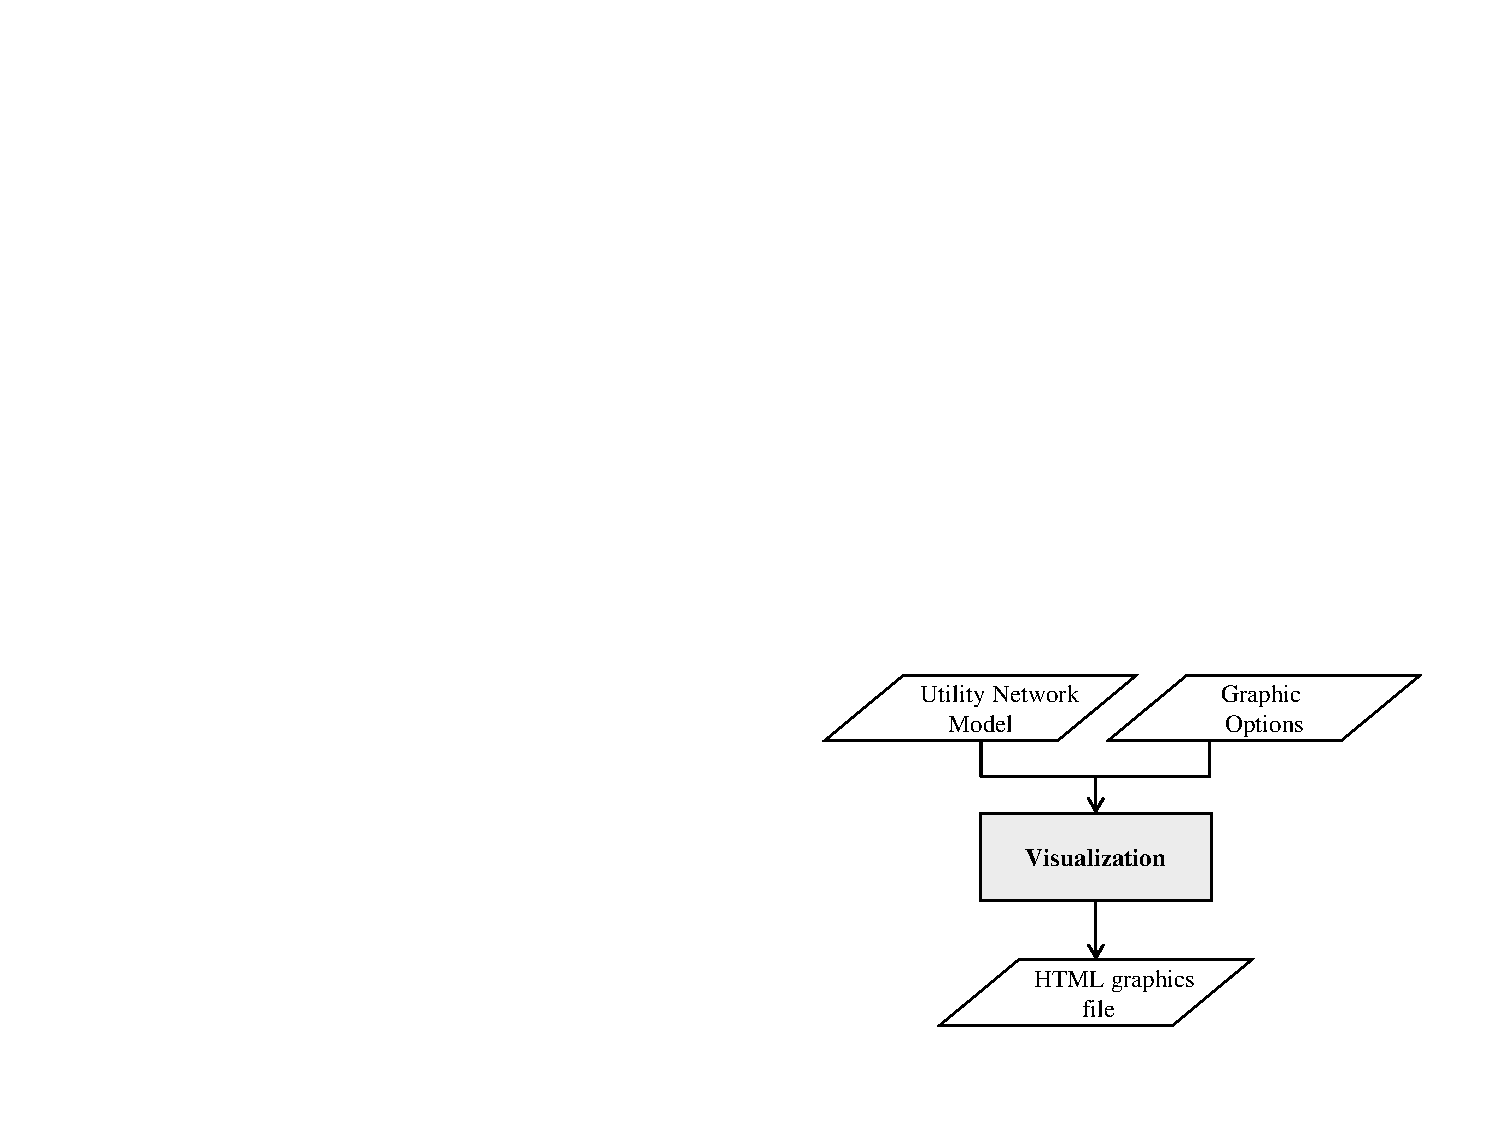
\includegraphics[scale=0.80]{graphics/visualization_flowchart.pdf}
  \caption{Visualization flowchart.}
  \label{fig:visualization-flowchart}
\end{figure}

\section{Color and Shape Options}
The color of a network element is specified using a six character hexadecimal (HEX) color code or using a 
predefined color name. HEX color codes can be found at various website, 
including \url{http://www.color-hex.com/color-wheel/}, and can be used to create 
any color between black (\#000000) and white (\#FFFFFF).
The following predefined colors can also be used in the the \code{visualization} 
subcommand.
\begin{unknownListing}
  Name    RGB           HEX
============================================
  red     [225,0,0]     \#FF0000 
  orange  [225,165,0]   \#FFA500
  yellow  [225,225,0]   \#FFFF00  
  green   [0,128,0]     \#008000
  blue    [0,0,225]     \#0000FF
  purple  [128,0,128]   \#800080
  black   [0,0,0]       \#000000
  white   [225,225,225] \#FFFFFF
  lime    [0,225,0]     \#00FF00
  navy    [0,0,128]     \#000080
  aqua    [0,225,225]   \#00FFFF
  teal    [0,128,128]   \#008080
  olive   [128,128,0]   \#808000
  maroon  [128,0,0]     \#800000
  fuchsia [225,0,225]   \#FF00FF
  silver  [192,192,192] \#C0C0C0
  gray    [128,128,128] \#808080
\end{unknownListing}

The shape of a network element is specified using one of the following predefined shapes, using 
either the long or short name.
\begin{unknownListing}
  Long Name    Short Name   
===========================
  circle        o
  square        s
  triangle      t
  diamond       d
  plus          +
  x		x
\end{unknownListing}

\section{Data from YAML Files}
Within the \code{visualization} WST configuration file, layers can be 
defined by 
(1) directly including the network element values, or
(2) referencing data in an external YAML file.

The following subset of a \code{visualization} WST configuration file 
demonstrates how element values are directly included in the layers block. 
\begin{unknownListing}
layers:
  locations: ['115', '101', '171']   
  file: null
\end{unknownListing}

The same data can be stored in an external YAML file and referenced in the 
\code{visualization} WST configuration file, as shown below. 
\begin{unknownListing}
layers:
  locations: '["flushing"]["nodes"][i]'
  file: data.yml
\end{unknownListing}
In this example, the referenced file, data.yml, contains the following information. 
\begin{unknownListing}
flushing:
  nodes: ['115', '101', '171']   
\end{unknownListing}

The WST subcommands (e.g., \code{sp}, \code{flushing}) that 
automatically run the \code{visualization} subcommand 
upon completion read data from external YAML files.

\section{\code{visualization} Subcommand}

The \code{visualization} subcommand is executed using the following command line:
\begin{unknownListing}
wst visualization <configfile> 
\end{unknownListing}
where \code{configfile} is a WST configuration file in the YAML format.  

The \code{---help} option prints information about this subcommand, such as usage,
arguments and a brief description:

\begin{unknownListing}
wst visualization --help
\end{unknownListing}

\subsection{Configuration File}

The \code{visualization} subcommand generates a template configuration file using the following command line:

\begin{unknownListing}
wst visualization --template <configfile>
\end{unknownListing}

The \code{visualization} WST template configuration file is shown in Figure \ref{fig:visualization_template}. 
Brief descriptions of the options are included in the template after the \# sign.  

\begin{figure}[H]
  \unknownInputListing{examples/visualization_config.yml}{}{1}{64}
  \caption{The \code{visualization} configuration template file.}
  \label{fig:visualization_template}
\end{figure}
  
\subsection{Configuration Options}

Full descriptions of the WST configuration options used by the \code{visualization} subcommand are listed below.
\begin{description}[topsep=0pt,parsep=0.5em,itemsep=-0.4em]
  \item[{network}]\hfill
  \begin{description}[topsep=0pt,parsep=0.5em,itemsep=-0.4em]
    \item[{epanet file}]\hfill
\\ The name of the EPANET 2.00.12 input (INP) file that defines the water distribution
                network model.
                
                Required input.
  \end{description}
  \item[{visualization}]\hfill
  \begin{description}[topsep=0pt,parsep=0.5em,itemsep=-0.4em]
    \item[{screen}]\hfill
    \begin{description}[topsep=0pt,parsep=0.5em,itemsep=-0.4em]
      \item[{color}]\hfill
\\The screen background color defined using a HEX color code or predefined color name.
                
                Optional input, default = white
      \item[{size}]\hfill
\\The screen size [width, height] in pixels.
                
                Optional input, default = [1000,600]
    \end{description}
    \item[{legend}]\hfill
    \begin{description}[topsep=0pt,parsep=0.5em,itemsep=-0.4em]
      \item[{color}]\hfill
\\The legend background color defined using a HEX color code or predefined color name.
                
                Optional input, default = white
      \item[{scale}]\hfill
\\The legend text size multiplier, real number.
                
                Optional input, default = 1.0
      \item[{location}]\hfill
\\The legend location [left, top] in pixels.
                
                Optional input, default = [10,10] (upper left)
    \end{description}
    \item[{nodes}]\hfill
    \begin{description}[topsep=0pt,parsep=0.5em,itemsep=-0.4em]
      \item[{color}]\hfill
\\The node color defined using HEX color code or predefined color name.
                The color will apply to junctions, reservoirs and tanks. If the 
                color is left blank, then junctions are black, reservoirs are 
                blue and tanks are green.
                
                Optional input, default = None
      \item[{size}]\hfill
\\The node size, real number.
                
                Optional input.
      \item[{opacity}]\hfill
\\The node opacity, real number between 0.0 (transparent) and 1.0 (opaque).
                
                Optional input, default = 0.6
    \end{description}
    \item[{links}]\hfill
    \begin{description}[topsep=0pt,parsep=0.5em,itemsep=-0.4em]
      \item[{color}]\hfill
\\The link color defined using HEX color code or predefined color name.
                The color will apply to pipes, pumps and valves. If the 
                color is left blank, then pipes are black, pumps are 
                yellow and valves are turquoise.
                
                Optional input, default = None
      \item[{size}]\hfill
\\The link size, real number.
                
                Optional input.
      \item[{opacity}]\hfill
\\The link opacity, real number between 0.0 (transparent) and 1.0 (opaque).
                
                Optional input, default = 0.6
    \end{description}
    \item[{layers}]\hfill
    \begin{description}[topsep=0pt,parsep=0.5em,itemsep=-0.4em]
      \item[{label}]\hfill
\\The layer label used in the legend. 
                
                Optional input, default = None
      \item[{locations}]\hfill
\\
                The data locations to plot over the network. Locations are specified
                using a list of EPANET IDs.
                
                Required input unless an external file is specified.
      \item[{file}]\hfill
\\The name of an external file that contains data to be used in the visualization.
                The file is in YAML format. 
                
                Required input unless 'locations' are specified.  
                Data from a file overrides data specified in 'locations'
      \item[{location type}]\hfill
\\The location type is used to indicate if the EPANET ID is of type 'node' 
                (junction, reservoir, tank) or 'link' (pipe, pump, valve).
                
                Optional input. If left blank, node is tested before link
      \item[{shape}]\hfill
\\The marker shape, used only for node type layers. The shape can
                be a single string, or a list of strings which is the same 
                length as the location data.
                
				Optional input, only used for node type layers, default = circle
      \item[{fill}]\hfill
      \begin{description}[topsep=0pt,parsep=0.5em,itemsep=-0.4em]
        \item[{color}]\hfill
\\The fill color defined using HEX color code or predefined color name.
                
                Optional input, default = None
        \item[{size}]\hfill
\\The fill size, real number.
                
                Optional input.
        \item[{opacity}]\hfill
\\The fill opacity, real number between 0.0 (transparent) and 1.0 (opaque).
                
                Optional input, default = 0.6
        \item[{color range}]\hfill
\\The fill color range used to scale line data.
                
                Optional input, default = [data min, data max]
        \item[{size range}]\hfill
\\The fill size range used to scale line data.
                
                Optional input, default = [data min, data max]
        \item[{opacity range}]\hfill
\\The fill opacity range used to scale line data.
                
                Optional input, default = [data min, data max]
      \end{description}
      \item[{line}]\hfill
      \begin{description}[topsep=0pt,parsep=0.5em,itemsep=-0.4em]
        \item[{color}]\hfill
\\The line color defined using HEX color code or predefined color name.
                
                Optional input, default = None
        \item[{size}]\hfill
\\The line size, real number.
                
                Optional input.
        \item[{opacity}]\hfill
\\The fill opacity, real number between 0.0 (transparent) and 1.0 (opaque).
                
                Optional input, default = 0.6
        \item[{color range}]\hfill
\\The line color range used to scale line data.
                
                Optional input, default = [data min, data max]
        \item[{size range}]\hfill
\\The line size range used to scale line data.
                
                Optional input, default = [data min, data max]
        \item[{opacity range}]\hfill
\\The line opacity range used to scale line data.
                
                Optional input, default = [data min, data max]
      \end{description}
    \end{description}
  \end{description}
  \item[{configure}]\hfill
  \begin{description}[topsep=0pt,parsep=0.5em,itemsep=-0.4em]
    \item[{output prefix}]\hfill
\\The prefix used for all output files.
                
                Required input.
    \item[{output directory}]\hfill
      \\The output directory to store the results.
    \item[{debug}]\hfill
\\The debugging level (0 or 1) that indicates the amount of debugging 
                information printed to the screen, log file and output yml file. 
                
                Optional input, default = 0 (lowest level).
  \end{description}
\end{description}


For additional control over the way that junctions, reservoir, tanks, pipes, pumps and valves are
displayed, the following YAML blocks can be added to the visualization configuration block.
The color, size and opacity of each element can be changed; and the element can
be added to the legend. These options will override the node and link blocks.
\begin{unknownListing}
  junctions:
    color: red  
    size: 5.0
    opacity: 0.5
  reservoirs:
    color: orange
    size: 12.0
    opacity: 1
  tanks:
    color: yellow
    size: 12.0
    opacity: 1
  pipes:
    color: green
    size: 3.0
    opacity: 0.5
  pumps:
    color: blue
    size: 3.0
    opacity: 1
  valves:
    color: purple
    size: 3.0
    opacity: 0.7
\end{unknownListing}
\subsection{Subcommand Output}

The \code{visualization} subcommand creates a HTML file 
named <output prefix>visualization\_output.html
that contains scalar vector graphics that can be opened in a Web browser.  
Two other files are created: 
(1) an output YAML file named <output prefix>visualization\_output.yml
that includes run date and CPU time, and 
(2) a log file named <output prefix>visualization\_output.log
that includes basic debugging information.

\section{Visualization Examples}\label{visualization_example}

An EPANET 2.00.12 network model input file (INP format) and a configuration file, which contain the
graphics options, are required to run the \code{visualization} subcommand.  
Several examples for visualization are given below.

\subsection{Example 1}

The first example customizes the color, size and opacity of the network
elements (junctions, reservoirs, tanks, pipes and pumps). The reservoir and 
tank colors are specified using HEX color codes. Additionally, the graphic
highlights five pipes and uses their diameter to scale the pipe width. 
All the data is supplied in the configuration file.  
The configuration file, visualization\_ex1.yml, for this example is shown in Figure \ref{fig:visualization_ex1}.  

\begin{figure}[h]
  \unknownInputListing{../../examples/visualization_ex1.yml}{}{1}{46}
  \caption{The \code{visualization} configuration file for example 1.}
  \label{fig:visualization_ex1}
\end{figure}

The example can be executed using the following command line:

\begin{unknownListing}
wst visualization visualization_ex1.yml
\end{unknownListing}

The resulting graphic is shown in Figure \ref{fig:visualization_graphic_ex1}.

\begin{figure}[h]
  \centering
  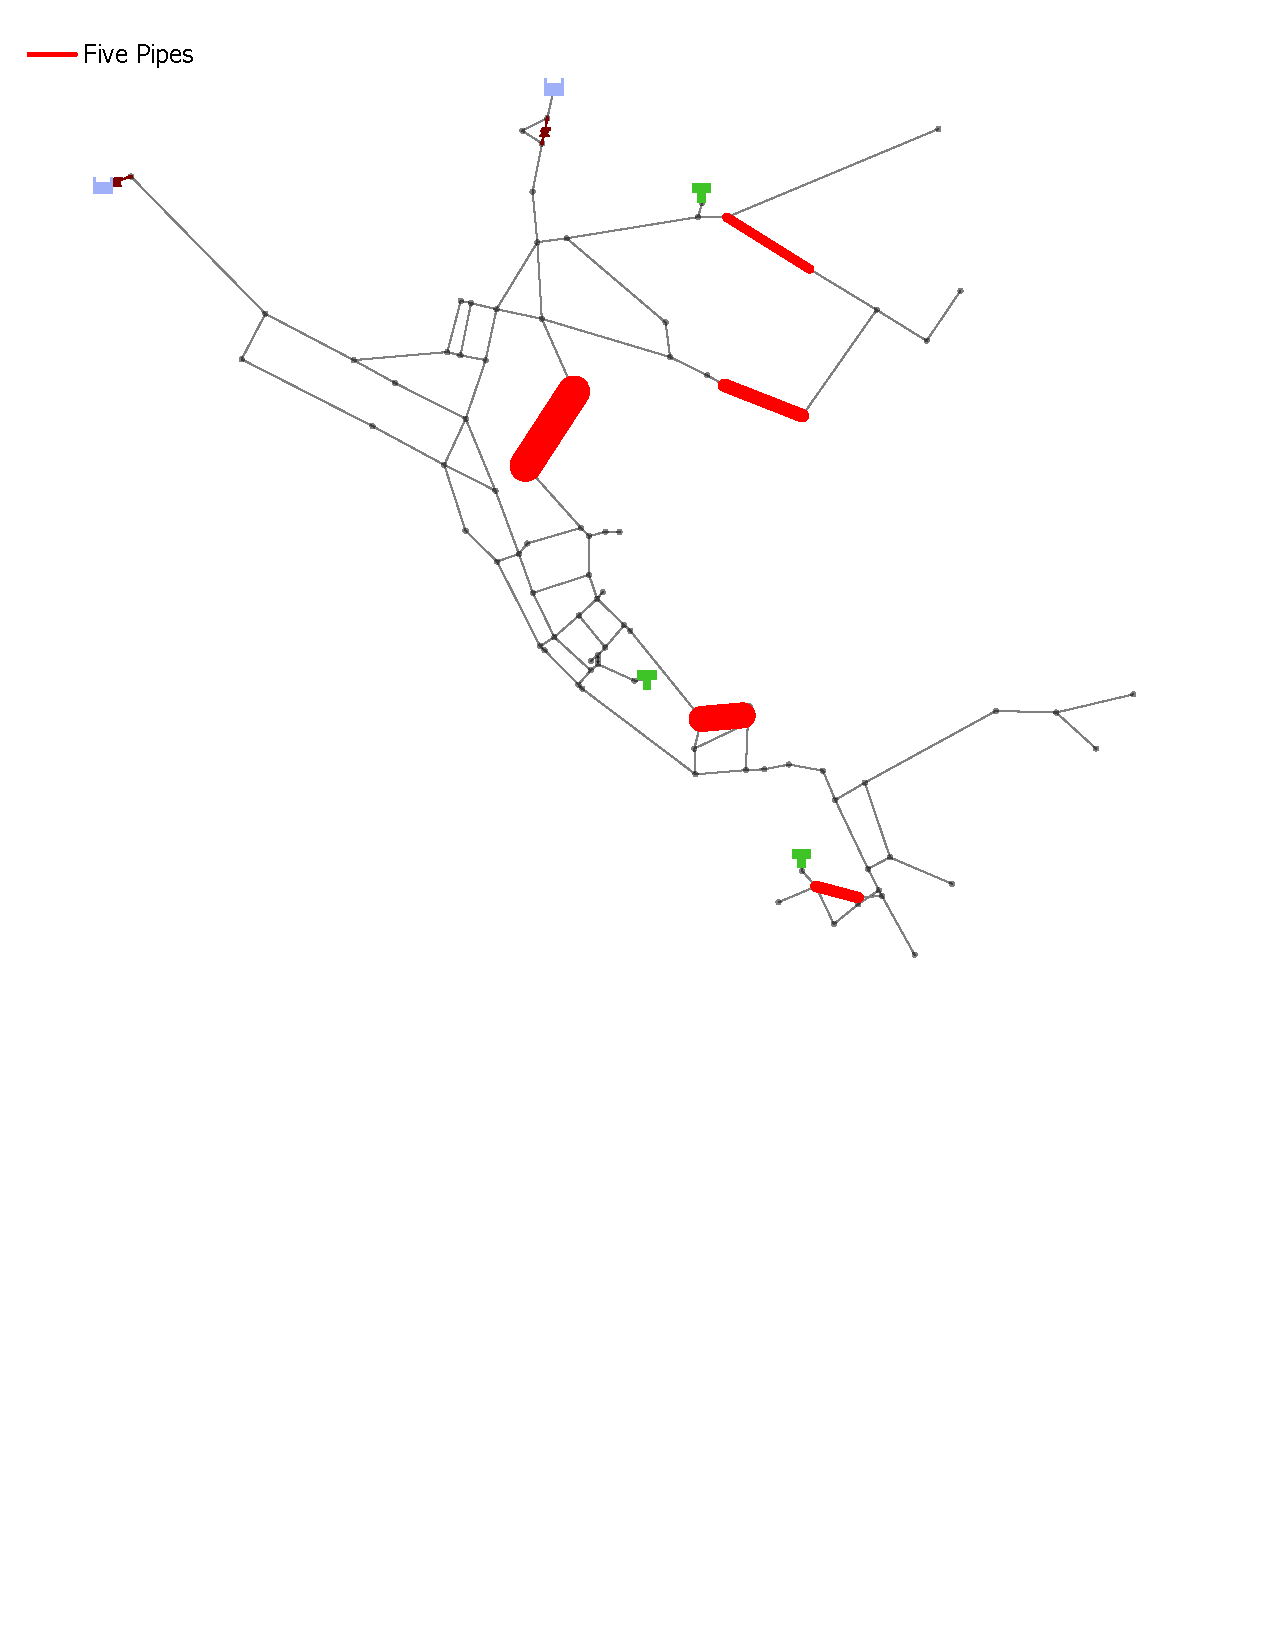
\includegraphics[scale=0.80]{examples/visualization_ex1.pdf}
  \caption{Graphic from \code{visualization} example 1.}
  \label{fig:visualization_graphic_ex1}
\end{figure}

\FloatBarrier 
\subsection{Example 2}

The second example uses an external data file to define locations and values to
be used in the network graphic.
The configuration file, visualization\_ex2.yml, for this example is shown in Figure \ref{fig:visualization_ex2}.  
The location file used in this example is shown in Figure \ref{fig:visualization_locations_ex2}. 
This example uses the pipe length to scale the size and opacity of the links and 
the base demand to scale the color and size of the nodes. This graphic 
shows that link 329 is very long compared to the other 30-inch diameter pipes and 
that node 109 has the largest base demand. The size range option in the configuration file   
is used to automatically scale the size and opacity of each layer. For example, 
the link length ranges from 1 to 45,500, but is scaled to a size range of 5 to 20.   
\begin{figure}[h]
  \unknownInputListing{../../examples/visualization_ex2.yml}{}{1}{38}
  \caption{The \code{visualization} configuration file for example 2.}
  \label{fig:visualization_ex2}
\end{figure}

\begin{figure}[h]
  \unknownInputListing{../../examples/Net3/Net3_locations.yml}{}{1}{5}
  \caption{The location file used in \code{visualization} example 2.}
  \label{fig:visualization_locations_ex2}
\end{figure}

The example can be executed using the following command line:

\begin{unknownListing}
wst visualization visualization_ex2.yml
\end{unknownListing}

The resulting graphic is shown in Figure \ref{fig:visualization_graphic_ex2}.

\begin{figure}[h]
  \centering
  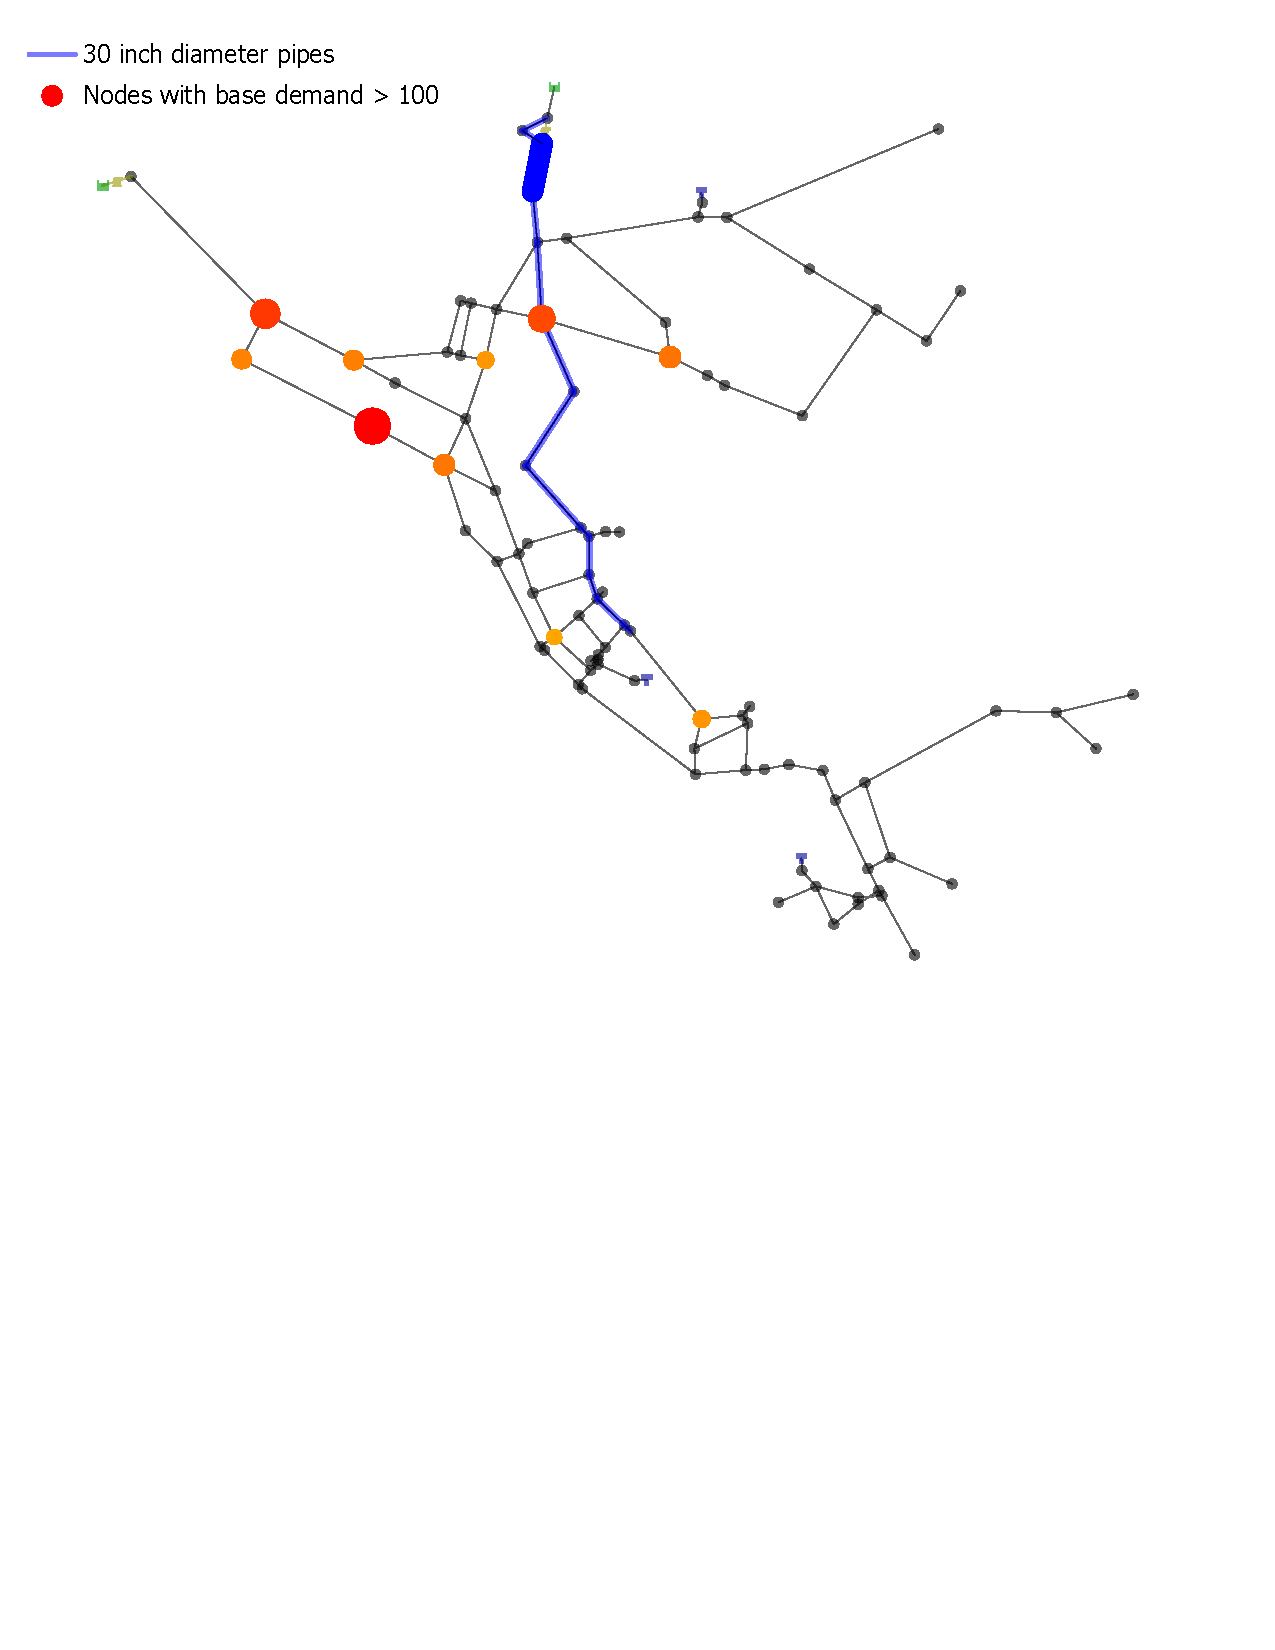
\includegraphics[scale=0.80]{examples/visualization_ex2.pdf}
  \caption{Graphic from \code{visualization} example 2.}
  \label{fig:visualization_graphic_ex2}
\end{figure}



  \chapter{Advanced Topics and Case Studies}
  \label{part2}
  This chapter provides more background information on the Merlion 
water quality model and discusses a few of the more advanced topics 
for the sensor placement problem. In addition, a few case study applications 
using the different WST subcommands are provided.

\section{Merlion Water Quality Model}\label{appendixMerlion} 
The Merlion water quality modeling framework is provided with WST to enable
fast multi-scenario simulations and solution of optimization problems that require
an embedded water quality model (e.g., booster placement with \code{booster\_mip}, source identification MIP formulation). 
In this section, the model equations and the calculations performed inside WST 
in order to generate a linear system of equations to describe the water
quality in a network are briefly described. The equations and the discretization process described in 
this section do not require any additional work from the user (except for selecting the merlion 
option in the configuration file). More details about the Merlion modeling framework is provided in \citep{Merlion12}.   
      
The model formulation ensures mass balances
at all junctions, pipes and tanks. The following mass balance equations
describe the transport of a species inside the network. For simplicity,
complete instantaneous mixing is assumed for the tanks, and plug flow
is assumed for the pipes.

\bigskip{}

\begin{equation}
c_{n}(t)=\dfrac{\sum_{i\in\Gamma_{n}^{O}(t)}Q_{i}(t)\hat{c}_{i}^{O}(t)-\sum_{i\in\Gamma_{n}^{I}(t)}Q_{i}(t)\hat{c}_{i}^{I}(t)+m_{n}(t)}{\sum_{i\in\Gamma_{n}^{O}(t)}Q_{i}(t)-\sum_{i\in\Gamma_{n}^{I}(t)}Q_{i}(t)+Q_{n}^{ext}(t)},\;\;\forall\;
n\in\mathbf{J} \label{eq:junctionbalance}
\end{equation}

\medskip{}

\begin{multline}
V_{n}(t)\dfrac{dc_{n}(t)}{dt}=\sum_{i\in\Gamma_{n}^{O}(t)}Q_{i}(t)\hat{c}_{i}^{O}(t)-\sum_{i\in\Gamma_{n}^{I}(t)}Q_{i}(t)\hat{c}_{i}^{I}(t)+m_{n}(t)\\
-\left[\sum_{i\in\Gamma_{n}^{O}(t)}Q_{i}(t)-\sum_{i\in\Gamma_{n}^{I}(t)}Q_{i}(t)+Q_{n}^{\mathrm{ext}}(t)\right]c_{n}(t),\;\;\forall\; n\in\mathbf{ST}\label{eq:tankbalance}
\end{multline}

\bigskip{}

\begin{equation}
\dfrac{\partial\hat{c}_{i}(x,t)}{dt}+u_{i}(t)\dfrac{\partial\hat{c}_{i}(x,t)}{dx}=0,\forall i\in\mathbf{P}\label{eq:pipebalance}
\end{equation}

where $c_{n}$ and $m_{n}$ denotes the concentration and mass injected at a node,
respectively. The variable $\hat{c}_{i}$ is the concentration inside pipe $i$ 
and $V_{n}$ is the volume of water inside tank $n$.
The variable $\mathbf{{J}}$ is a set of all junctions, $\mathbf{{ST}}$
is a set of all storage tanks and $\mathbf{{P}}$ is a set of all
pipes. The variable $Q$ denotes volumetric flow rates that are pre-calculated using
EPANET 2.00.12 and are assumed to be constant over each hydraulic time step.
The flow rate of a known external source entering a node is also pre-calculated
and is denoted by $Q_{i}^{\mathrm{ext}}$. The variable $\Gamma_{n}^{O}$ represents the
set of all pipes with flow going away from node $n$. Similarly,
$\Gamma_{n}^{I}$ represents the set of all pipes with flow coming
into node $n$. 

Equation~\ref{eq:junctionbalance} represents a set of algebraic equations
dependent on time alone and Equation~\ref{eq:tankbalance} represents
a set of ordinary differential equations (ODEs) also dependent on time alone. Therefore, these two equations
can be discretized in time. However, discretizing Equation~\ref{eq:pipebalance},
which are partial differential equations (PDEs), in both time and space would lead to a prohibitively
large model. Instead, these pipe balance PDEs are replaced using an origin-tracking
algorithm. This algorithm is based on the Lagrangian method; however,
instead of tracking concentration values as packets of water moving
through the network, the origin-tracking algorithm tracks the originating
node and time step of each packet as it enters a pipe (see Figure \ref{fig:origin_figure}). 
Once the water packet exits the pipe, equations are written relating
the concentration of the pipe inlet and outlet to the concentration
of connected nodes based on time delay. These time delay expressions
are formulated for each pipe independently. Therefore, the algorithm
scales favorably for a large water distribution system having a linear
computational cost as the size of the network increases. 

\begin{figure}[!h]
\begin{center}
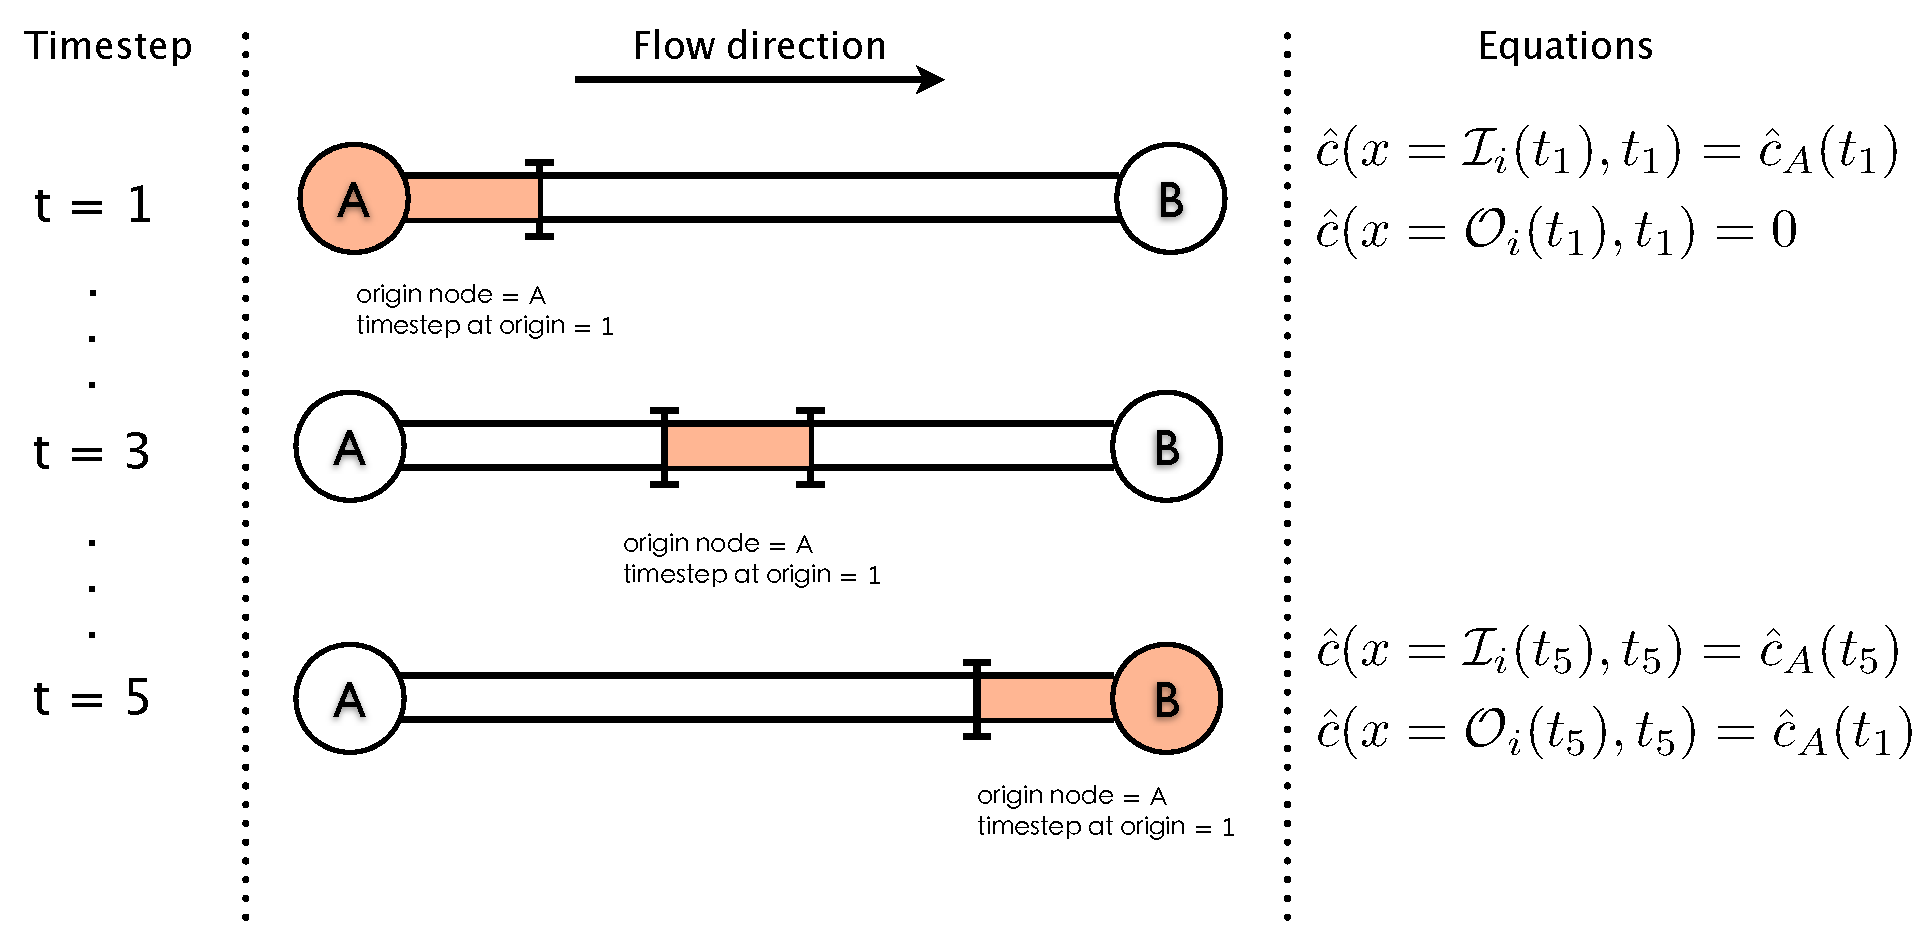
\includegraphics[scale=0.38]{graphics/origin_figure.pdf}\caption{Illustration of the origin tracking algorithm.}
\label{fig:origin_figure}
\end{center}
\end{figure}


By calculating time delay expressions, a very large but sparse linear
system of equations is generated that relates 
%The time delay expressions are included in the mass balance equations
%to form a large but very sparse linear system relating 
input injections ($m$)
from all nodes and time steps to output concentrations ($c$) from
all nodes and time steps.

\begin{equation}
Gc=Dm\label{eq:Merlion_Model}
\end{equation}


Unlike black box simulations, this linear model can be extended and
embedded inside other numerical applications. For example, the water quality model can be
embedded inside a mathematical programming formulation for applications
like booster placement, source inversion and optimal grab sampling. 

After formulating the linear system, performing a tracing simulation
is straightforward. First, an injection profile ($m$) is specified.
Then, the system is factorized and finally backsolved for the network
concentration profile $c$. This process is fast, and even more efficient
when simulating a large ensemble of tracing simulations. In this case,
the system is factorized once, and a backsolve is performed for each
simulation. To get additional speedup, a tailored solver is also provided
that takes advantage of the structure of the linear system by permuting
matrix $G$ into lower triangular, which removes the need for any
factorization. The tailored solver also utilizes the Basic Linear
Algebra Sub-routines (BLAS) library to perform multiple backsolves
(corresponding to multiple injection scenarios) more efficiently. 
For additional information about Merlion, refer to \citet{Merlion12}. 
%\mathbf{NOTE: Merlion currently only supports time based controls. 
%All EPANET networks INP files provided with WST have been modified by 
%converting all conditional controls to time based controls. This was 
%done by running the hydraulics and finding the first time at which a 
%conditional control was trigger and then enforcing a time based control 
%at the closest earlier hydraulic time step.} 

\newpage

\section{Average-case Sensor Placement}\label{chap:pmedian} 

The \code{sp} subcommmand can design a sensor network for contamination
warning systems (CWSs) using a variety of different optimization
formulations. The most widely studied sensor placement formulation
for CWS design is to minimize the expected impact of an ensemble
of contamination incidents given a sensor budget. This formulation
has also become the standard formulation for \code{sp}, because it
can be effectively used to select sensor placements in large water
distribution networks. This chapter provides a variety of examples
that illustrate the application of the \code{sp} subcommand for this optimization formulation.
Sensor placement formulation and examples illustrating common use of \code{sp} are included in Chapter~\ref{chap:sp}.

\subsection{Computing a Bound on the Best Sensor Placement Value}\label{solvers_solvers2a}

A mixed-integer program (MIP) solver like GLPK provide upper and lower bounds on the value
of the final solution. For large water distribution systems, it
might be prohibitively expensive to perform optimization with a MIP
solver. However, computing a lower bound with these solvers might
be practical even for large water distribution systems.

The configuration file shown in Figure \ref{fig:sp_bound}
defines a sensor placement problem with the compute bound option set to true in the 
problem block. This option indicates that the goal for the optimizer is to compute a lower bound 
on the globally optimal solution, rather than finding a sensor placement. 
All other options are those previously defined in example 3 of the Sensor 
Placement Examples (See Section~\ref{sp_example}).

\begin{figure}[h]
  \unknownInputListing{examples/sp/sp_bound.yml}{}{1}{28}
  \caption{The \code{sp} configuration file using the GLPK solver to compute a lower bound.}
  \label{fig:sp_bound}
\end{figure}

The YAML output file in Figure \ref{fig:sp_bound_output} contains the lower bound value. 
This is the same value as the solution generated by the GRASP heuristic in 
example 3 of the Sensor Placement Examples (See Section~\ref{sp_example}). 
In this manner, a MIP solver can be used to evaluate whether a heuristic 
sensor placement is near-optimal.

\begin{figure}[h]
  \unknownInputListing{examples/sp/sp_bound_output.yml}{}{1}{14}
  \caption{The \code{sp} YAML file with the lower bound from the GLPK solver.}
  \label{fig:sp_bound_output}
\end{figure}

The Lagrangian heuristic leverages the structure of the eSP model (Equations~\ref{eqn:eSP}) to
guide its search. Specifically, this heuristic computes the optimal values for the 
integer relaxation of eSP and then applies a randomized rounding technique.
As a consequence, this heuristic can also be used to compute bounds on the value of 
sensor placement in a manner that is similar to a MIP solver.
The configuration file in Figure 
\ref{fig:sp_bound_lag} uses the Lagrangian solver to determine the sensor placement 
for example 3 of the Sensor Placement Examples (See Section~\ref{sp_example}). 

\begin{figure}[h]
  \unknownInputListing{examples/sp/sp_bound_lag.yml}{}{1}{28}
  \caption{The \code{sp} configuration file using the Lagrangian solver.}
  \label{fig:sp_bound_lag}
\end{figure}

The YAML output file in Figure \ref{fig:sp_bound_lag_yaml} shows
the results of sensor placement using the Lagrangian solver for
example 3 of the Sensor Placement Examples (See Section~\ref{sp_example}).
It contains the sensor locations (EPANET IDs), the objective value
(the impact metric value), the lower bound on this objective as
well as the upper bound, which is the same as the objective value.
The sensor locations identified are nodes 139,
161, 191 and 208. The mean extent of contamination (EC) impact for
this design is approximately 9889 pipe feet contaminated. The lower
bound is approximately 9819 pipe feet contaminated, which is greater than the
bound computed by GLPK. This illustrates the fact that the bounds computed
by the Lagrangian solver are weaker than those computed by a MIP solver.

\begin{figure}[h]
  \unknownInputListing{examples/sp/sp_bound_lag_output.yml}{}{1}{14}
  \caption{The \code{sp} YAML file with the lower bound from the Lagrangian solver.}
  \label{fig:sp_bound_lag_yaml}
\end{figure}

As with MIP solvers, the Lagrangian solver can also be used to simply compute this lower bound.  
The configuration file in Figure \ref{fig:sp_bound_only_lag} shows an example of using the 
compute bound option in the problem block with the Lagrangian solver.

\begin{figure}[h]
  \unknownInputListing{examples/sp/sp_bound_only_lag.yml}{}{1}{29}
  \caption{The \code{sp} configuration file using the Lagrangian solver and the compute bound option.}
  \label{fig:sp_bound_only_lag}
\end{figure}

\subsection{Managing Sensor Placement Locations}\label{solvers_solvers2c}

By default, the \code{sp} subcommand assumes that all node locations in
a water distribution network are feasible sensor locations. 
In practice, sensors cannot be practically installed in many locations without
significant cost and inconvenience. The location block in the 
configuration file is used to specify options for declaring feasible and infeasible
node locations in the network. Additionally, the location block
can be used to declare node locations as fixed, where a sensor must be
placed, and unfixed, where a sensor cannot be located.

A location block consists of a list of declarations that are
interpreted in their order within the configuration file. Each
declaration consists of a dictionary with a single key, whose value
is either a string or list of EPANET node IDs. For example, the following location
block declares a list of infeasible node locations:
\unknownInputListing{examples/sp/fixed1.yml}{block}{22}{28}

The impact of infeasible sensor locations on the results
for example 1 of the Sensor Placement Examples (See
Section~\ref{sp_example}) is shown in following example. The solution from this example placed
sensors at nodes 113, 121, 141, 163 and 209 and the mean extent of
contamination (EC) for this sensor design was 8655. If these nodes
were listed as infeasible sensor locations (as shown in the location
block above) in the configuration file, the new sensor locations
are nodes 111, 119, 169, 207 and 237. The mean EC for this new
solution is 8932 which is worse than the initial design; this
reflects the fact that a sensor design that can use any location
will be better than a sensor design that can use a limited set of
locations.


\subsection{Limited-\/Memory Sensor Placement Techniques}\label{solvers_solvers5}

Controlling the memory used by optimizers is a critical issue when
solving large sensor placement formulations. This is a particular
challenge for MIP methods, but both the GRASP and Lagrangian
heuristics can exceed a workstation's memory when solving very large
problems. The \code{sp} subcommand supports a variety of mechanisms
that reduce the problem representation size while preserving the
structure of the sensor placement problem. These techniques include:
scenario aggregation and filtering, feasible locations, witness
aggregation, skeletonization and explicit memory management.

\paragraph{Scenario Aggregation:}
Scenario aggregation compresses the data in an impact file while
preserving its fundamental structure. This strategy is effective
when optimizing for mean performance objectives. Scenario aggregation
is performed with the \code{scenarioAggr} command, which is described
in Section~\ref{scenarioAggrExecutable}.

\paragraph{Filtering Impacts:}
Filtering impacts can also reduce memory requirements for sensor
placement by reducing the size of the impact files. Filtering can
limit the sensor placement formulation to only consider contamination
incidents that are sufficiently bad in the worst-\/case. Filtering
is performed with the \code{filter\_\-impacts} executable, which
is described in Section~\ref{filter_impactsExecutable}

\paragraph{Feasible Locations:}
Limiting the feasible locations is another strategy to reduce memory
requirements. The size of the sensor placement formulation
decreases as the number of feasible locations decreases. The
location block option described in Section~\ref{solvers_solvers2c}
can be used to specify the set of feasible locations.

\paragraph{Witness Aggregation:}
Witness aggregation limits the size of the sensor placement formulation
by aggregating the decision variables that witness a contamination
incident. By default, variables that witness contamination incidents
with the same impact are aggregated, and this typically reduces the
MIP constraint matrix by a significant amount. Further reductions
perform more aggressive aggregations that create an approximate
sensor placement formulation.

Witness aggregation is specified using an \code{aggregate} block
in the \code{sp} configuration file. A named aggregation block
specifies the type of aggregation, the aggregation limit value and
the associated impact data. For example:\newline
\begin{minipage}{\textwidth}
\begin{unknownListing}
aggregate: 
- name: agg1
  type: PERCENT
  goal: impact1
  value: 0.125
  conserve memory: 0
  distinguish detection: 0
  disable aggregation: [0]
\end{unknownListing}
\end{minipage}

The following table illustrates the use of the two witness aggregation
options when optimizing the mean extent of contamination: aggregation
type = PERCENT and aggregation type = RATIO. The RATIO aggregation
type can be used with distinguish detection option to help with
aggregation. The second line of data in this table is the default
aggregation, which has about half as many non-\/zero values in the
MIP constraint matrix. Both the percent and ratio aggregation
strategies effectively reduce the problem size while finding
near-\/optimal solutions.

\begin{center}
\begin{tabularx}{\textwidth}{|l|l|c|r|r|} \cline{1-5}
Aggregation Type & Aggregation Value & Binary Variables & MIP Nonzeros&Solution Value  \\\cline{1-5}
None&NA&97&220736&8525  \\\cline{1-5}
PERCENT&0.0&97&119607&8525  \\\cline{1-5}
PERCENT&0.125&97&49576&9513  \\\cline{1-5}
RATIO&0.125&97&12437&10991  \\\cline{1-5}
\end{tabularx}
\end{center} 

\paragraph{Skeletonization:} 
Another option to reduce the memory
requirement for sensor placement is to reduce the size of the network
model through skeletonization. Skeletonization groups neighboring
nodes based on the topology of the network and pipe attributes.
Section~\ref{skelExecutable} describes the \code{spotSkeleton}
executable, which provides techniques for branch trimming, series
pipe merging and parallel pipe merging. These techniques eliminate
pipes and nodes that have little effect on the overall hydraulics
of the system. This effectively contracts a connected piece of the
network into a single node, called a supernode. Skeletonized
networks can be used to define geographic proximity in a two-tiered
sensor placement approach for large network models~\citep{KliPhiJan13}.

\paragraph{Explicit Memory Management:}
The GRASP heuristic has several options for controlling how memory 
is managed. The \code{grasp-\/representation} solver option can be used to 
control how the local search steps are performed. By default, a dense matrix is 
precomputed to perform local search steps quickly, but a sparse matrix can be 
used to perform local search with less memory. Also, the GRASP heuristic can be 
configured to use the local disk to store this matrix.


\subsection{Evaluating a Sensor Placement}\label{solvers_solvers6}

Sensor placements can be evaluated based on an impact assessment of possible contaminant incidents.  
The \code{evalsensor} executable measures the performance of each sensor placement
with respect to the set of possible contamination locations. This analysis
assumes that probabilities have been assigned to these contamination
locations. If no probabilities are given, then uniform probabilities
are used. The \code{evalsensor} executable takes sensor placements in a sensor placement 
file and evaluates them using data from one or more impact files.
Sensor placement files are generated using the \code{sp} subcommand, and the file format is described 
in File Formats Section \ref{formats_sensorPlacementFile}. Impact files 
are generated using the \code{sim2Impact} subcommand, and the file format is described 
in the File Formats Section \ref{formats_impactFile}. Additional information on 
\code{evalsensor} can be found in the Executable Files Section \ref{evalsensorExecutable}.

The following example demonstrates the use of \code{evalsensor} using the sensor 
network design from Section~\ref{sp_example}.
The \code{evalsensor} command for this example is executed using the following command:

\begin{unknownListing}
evalsensor --nodemap=Net3.nodemap Net3_ec.sensors Net3_ec.impact Net3_mc.impact
\end{unknownListing}

This example generates output shown in Figure \ref{fig:evalsensor_ex1_screen_output}.

\begin{figure}[h]
  \unknownInputListing{examples/sp/evalsensor_ex1_screen_output.txt}{}{1}{29}
  \caption{The \code{evalsensor} example output.}
  \label{fig:evalsensor_ex1_screen_output}
\end{figure}

The \code{evalsensors} command can also evaluate a sensor placement in the 
case where sensors can fail, and there is some small number of different classes 
of sensors (grouped by false negative probability). This information is specified 
by an imperfect sensor class file and an imperfect junction class file, which are defined in 
Sections~\ref{formats_sensorClass} and~\ref{formats_junctionClass}, 
respectively. The imperfect sensor class (sc) file, \code{Net3.imperfectsc}, specifies different 
categories of sensor failures. Sensors of class 1 have a 
false negative probability of 25\%, sensors of class 2 have a probability of 50\%, 
class 3 have a 75\% probability and class 4 100\%. 

\lstinputlisting[]{../../examples/Net3/Net3.imperfectsc}

Once failure classes are defined, the nodes of the network are assigned 
to failure classes by using a imperfect junction class (jc) file. The beginning of the 
imperfect junction class file Net3.imperfectjc is shown below.

\lstinputlisting[firstline=0,lastline=10]{../../examples/Net3/Net3.imperfectjc}

Given the junction classes, \code{evalsensor} is used to determine the 
expected impact of a sensor placement, given that sensors might fail. 
The following command line executes \code{evalsensor} with specified failure probabilities:

\begin{unknownListing}
evalsensor --nodemap=Net3.nodemap --sc-probabilities=Net3.imperfectsc \
    --scs=Net3.imperfectjc Net3_ec.sensors Net3_ec.impact
\end{unknownListing}

This example generates output shown in Figure \ref{fig:evalsensor_ex2_screen_output}.

\begin{figure}[h]
  \unknownInputListing{examples/sp/evalsensor_ex2_screen_output.txt}{}{1}{18}
  \caption{The \code{evalsensor} output using sensor failure probabilities.}
  \label{fig:evalsensor_ex2_screen_output}
\end{figure}

The mean extent of contamination impact changes dramatically 
if sensors are allowed to fail. The original solution was 
misleading if sensors fail according to the assigned probabilities. 
With sensor failures, the expected impact is much higher.

\newpage

%\chapter{Sensor Placement: Advanced Topics}\label{chap:spadvanced} 
%\input{sp-advanced}

\section{Source Identification with Grab Samples Case Study}\label{chap:inversionCase} 
\label{inversion_case_study}
The following case study illustrates how the \code{inversion} and \code{grabsample} subcommands 
can be used in tandem to perform multiple cycles of source inversion calculations as more and more measurement data becomes available. 
The solution approach integrates iterative sampling strategy for finding the contamination source using discrete measurements 
obtained from manual grab samples taken during different sampling cycles.  
Figure \ref{fig:inversion_flowchart} illustrates the source inversion and grab sample strategy. 
A contamination incident is first suspected given a customer inquiry or detection from a fixed continuous 
sensor in the Contamination Warning System (CWS). 
At this stage, a team is sent out to gather manual grab samples at and around the location of first detection. 
Discrete yes/no measurements from these manual grab samples along with the measurement from CWS 
are then used to identify the potential sources of the contamination incident.
Since the inversion problem is an ill-posed problem, the solution will generally be non-unique. 
A set of likely locations can be identified and the \code{grabsample} subcommand can be used 
to determine the location of the next manual grab samples. The source inversion is performed again using the new information. 
This cycle of collecting manual grab samples and performing source inversion is continued until the true injection location(s) is identified. 
\begin{figure}[!ht]
\begin{center}
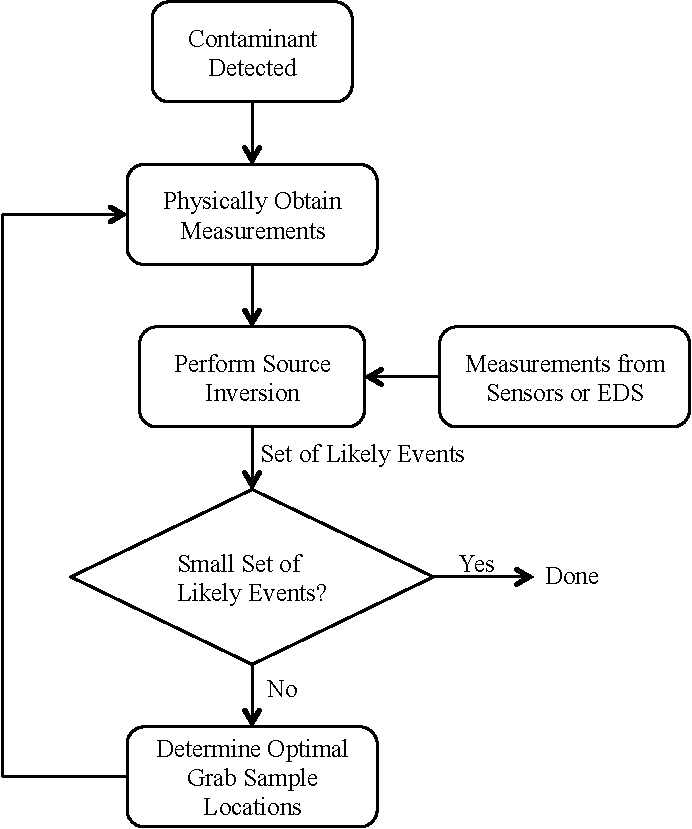
\includegraphics[scale=0.6]{graphics/inversion_strategy.pdf}
\caption{Illustration of the source inversion and grab sample cycling strategy.}
\label{fig:inversion_flowchart}
\end{center}
\end{figure}

\subsection{Case Study}
Since real system data is not available, the \code{measuregen}
executable is used to generate simulated data for the contamination incident in the following case study.  In this simulation, 
a conservative contaminant is injected into node 163 of EPANET
Example Network 3 (Net3) starting at 8 AM.  The Bayesian probability
based formulation [\ref{sec.bayesian_algorithm}] is used in
the \code{inversion} subcommand to identify the possible contamination
sources. Figure \ref{fig:case_study_setup} shows the fixed sensor
locations in blue while the original contamination location is shown
in red.  The CWS consists of five fixed sensors that provide
measurements every 15 minutes (set as a command line option in \code{measuregen}).

\begin{figure}[ht!]
\begin{center}
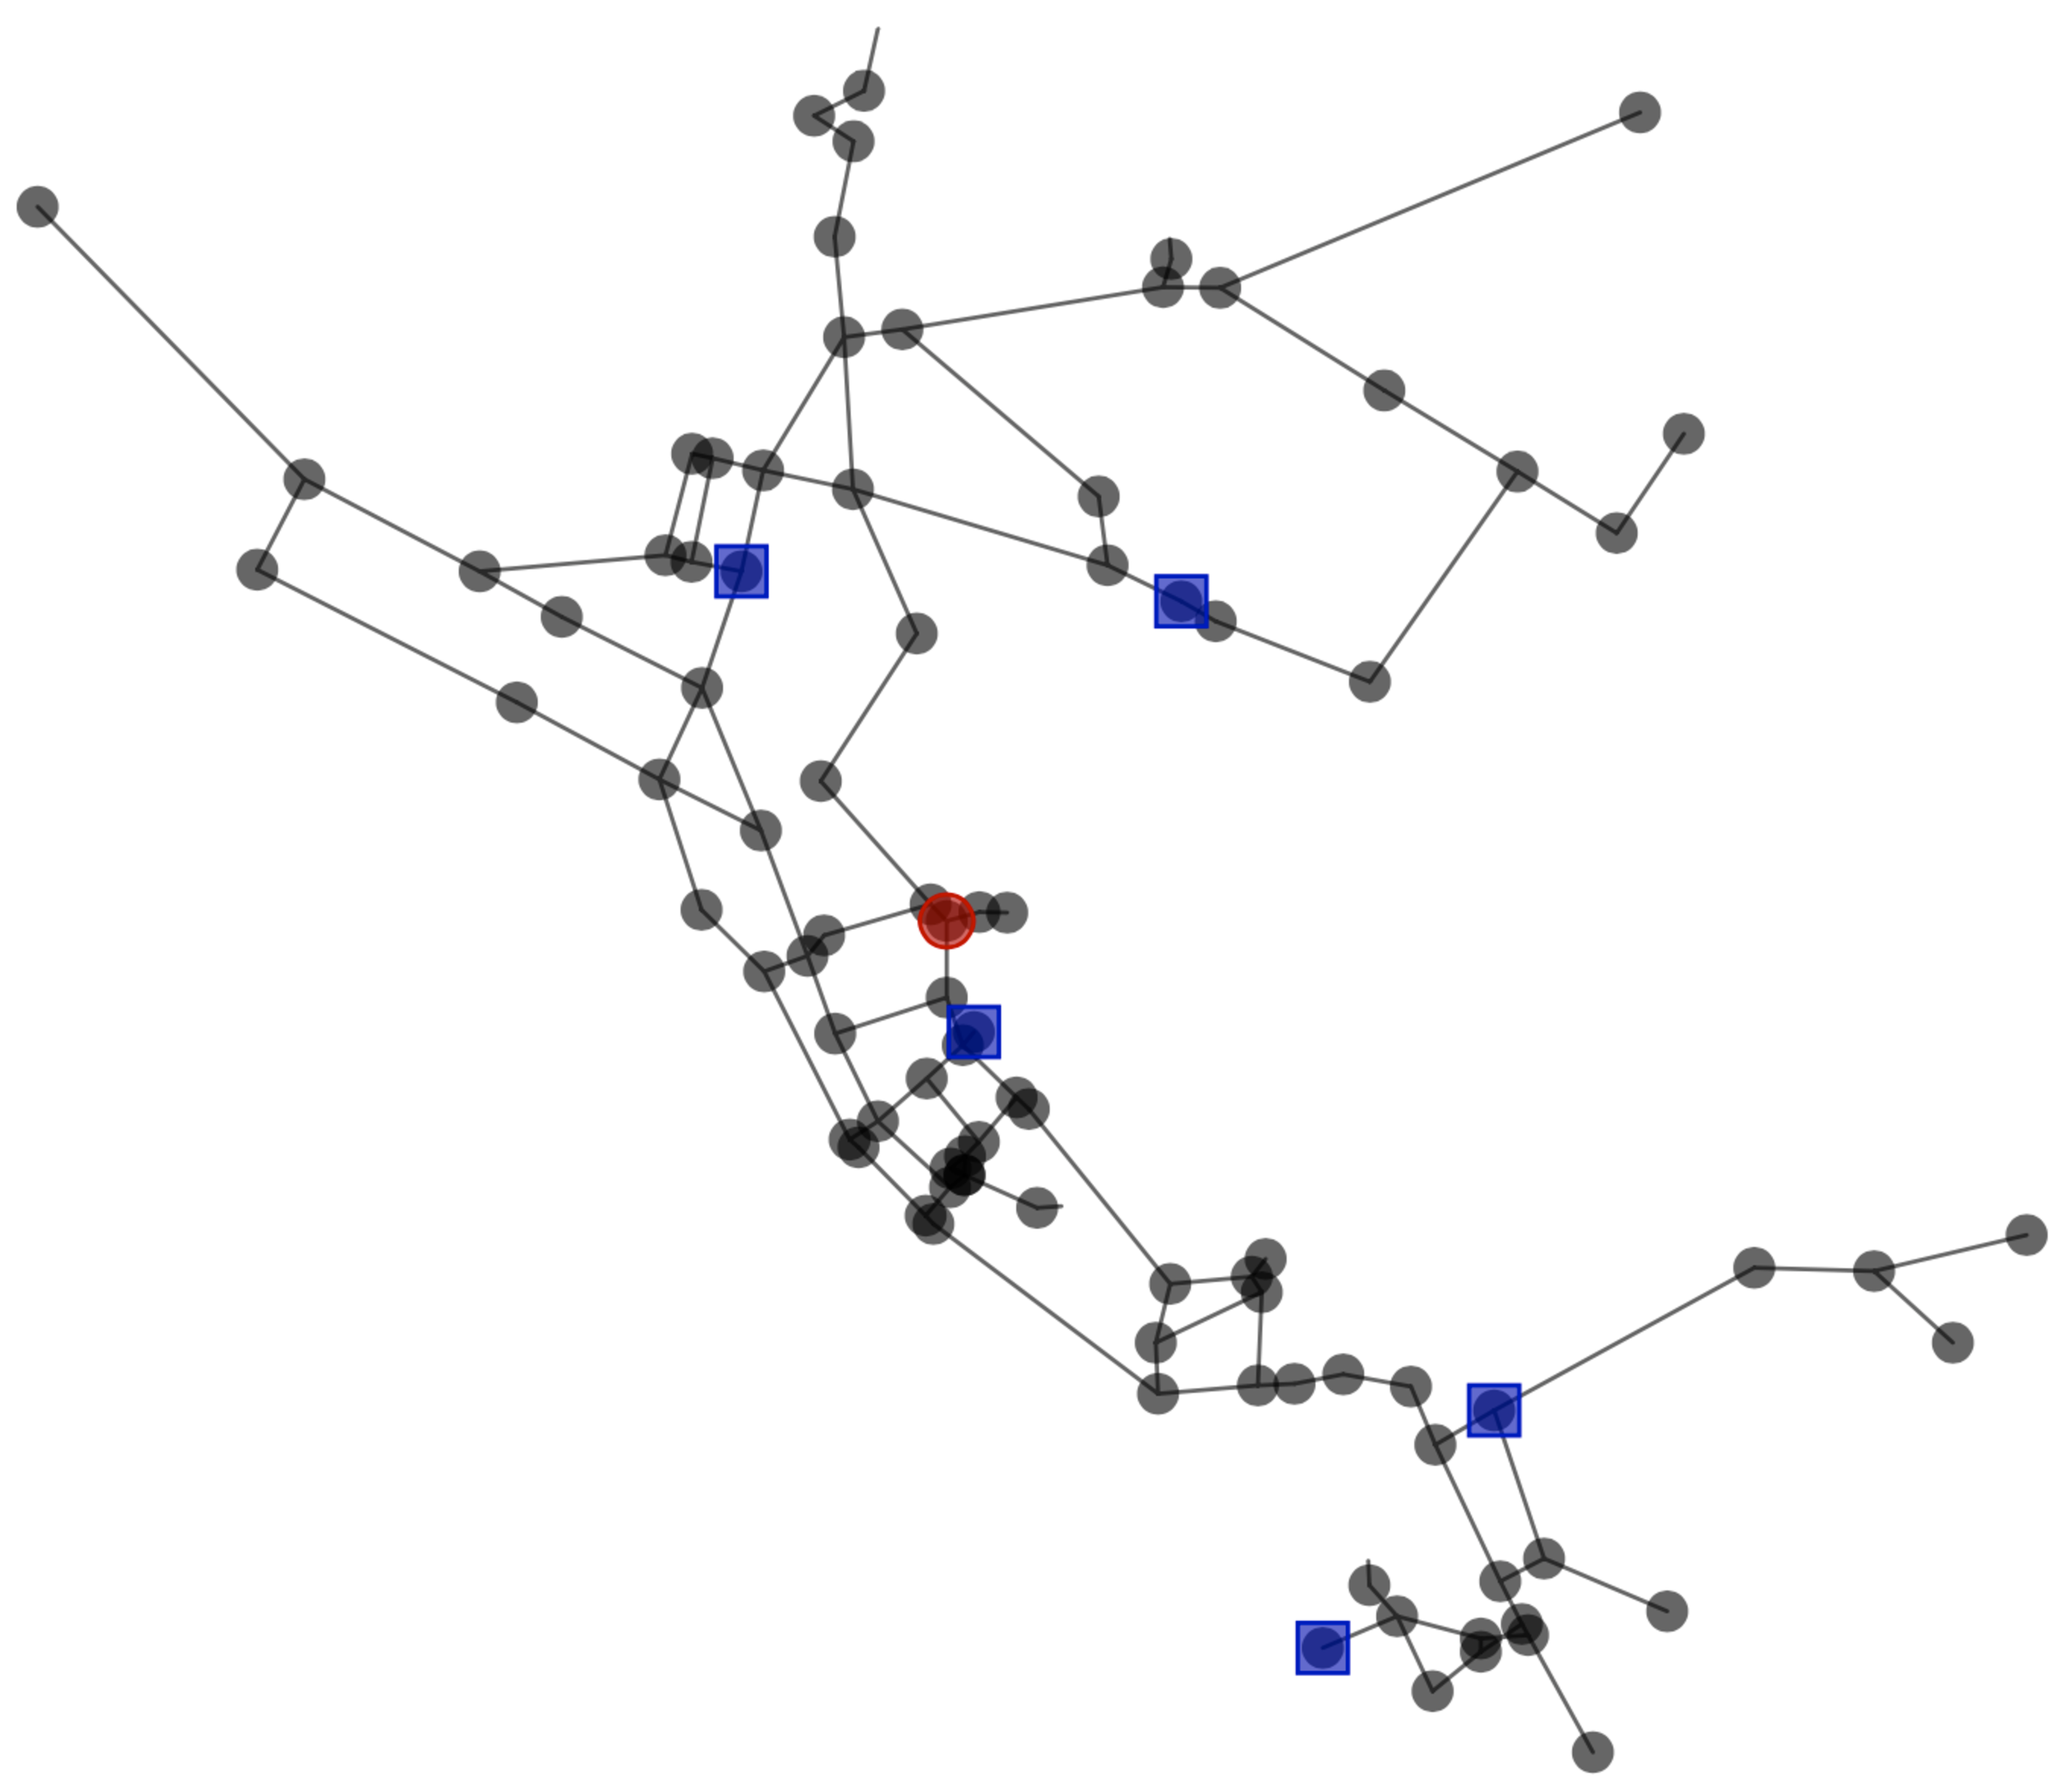
\includegraphics[scale=0.25]{graphics/inversion_cs_setup.pdf}
\caption{Fixed sensors (blue) and contamination location (red) for case study.}
\label{fig:case_study_setup}
\end{center}
\end{figure}

All the files required for this case study are provided in the \code{examples/case\_studies/inversion} folder.
  
The case study is a composed of three cycles of source inversion and grab sampling to reduce the number of possible contamination source 
locations. During each cycle, the \code{inversion} subcommand uses the following data:
\begin{itemize}
\item Net3.inp - EPANET Example Network 3 input (INP) file.
\item MEASURES.dat - Measurements file binary (yes/no) results from fixed sensors and grab samples (generated using \code{measuregen} executable).
\item \textit{<output\_prefix>}\_Likely\_Nodes.dat - Likely nodes file containing a list of feasible nodes to consider as possible contamination source nodes. 
This file is only used in cycles 2 \& 3. 
\end{itemize}      
The \code{inversion} subcommand outputs a YAML file with a list of possible contamination sources. 
A TSG file is also created that provides information about the possible contamination incidents. This file 
can be used in the \code{grabsample} subcommand. Thereafter, Cycles 1 \& 2 use the following data to determine optimal sample location:

\begin{itemize}
\item Net3.inp - EPANET Example Network 3 input (INP) file.
\item \textit{<output\_prefix>}\_profile.tsg - TSG file which contains a list of likely injections obtained 
from the \code{inversion} subcommand from the preceding cycle.
\item Sample time - Time in the future when the samples are expected to be taken. This is generally the current time 
plus the time it would take the sample teams to obtain measurements. 
\item fixed\_sensors.dat - List of fixed continuous sensor locations. This is used to avoid fixed sensors being selected
as grab sample locations.  

\end{itemize}

\subsection{Cycle 1}
At 8:15 AM, the sensor located at node 167 detects abnormal water quality. Further confirmation is made with another positive 
measurement at 8:30 AM. At this point, the measurement data from the past 8 hours is used to perform source inversion. 
The \code{inversion} subcommand identifies 24 possible injection locations as shown in red 
in Figure \ref{fig:case_study_cycle1}. The \code{grabsample} subcommand is then used to identify additional measurement 
locations that will reduce the number of possible injection locations. 
The utility has three teams available to gather manual grab samples and it takes 30 minutes for each team to 
obtain the manual samples. The \code{grabsample} subcommand identifies the three optimal grab sample locations 
shown in blue and the possible injection nodes in red in Figure \ref{fig:case_study_cycle1}.             

\begin{figure}[!ht]
\begin{center}
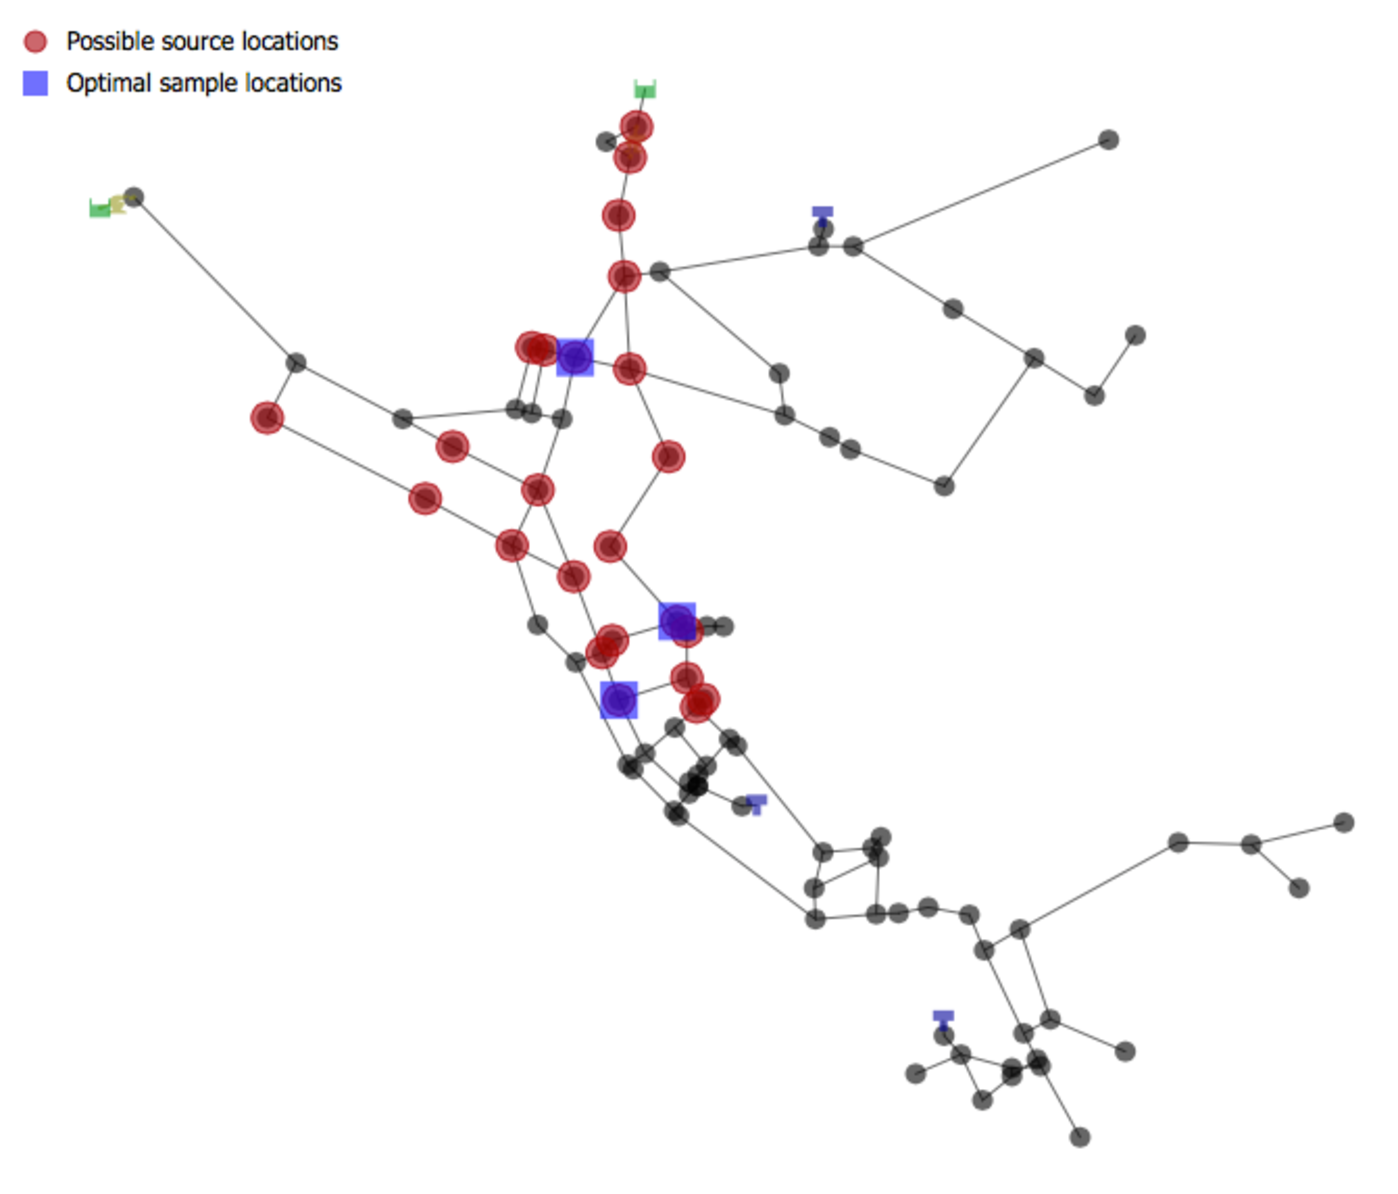
\includegraphics[scale=0.6]{graphics/inversion_cs_cycle1.pdf}
\caption{Cycle 1 identified optimal grab sample locations (blue).}
\label{fig:case_study_cycle1}
\end{center}
\end{figure}

The files required and generated during this cycle of source inversion and grab sample 
are provided in the \code{examples/case\_studies/inversion/Cycle1} folder. 

\subsection{Cycle 2}
In the 30 minutes that the sampling teams take to get manual grab sample measurements from the locations identified in Cycle 1, 
new measurements are also available from the fixed sensors in the CWS. It is assumed that
the sampling teams have field instruments that can provide them with a yes/no indication of the
presence or absence of a contaminant.  
At 9:00 AM, these new measurements are used to perform source inversion again. 
This time the \code{inversion} subcommand identifies seven possible injection locations as shown in Figure \ref{fig:case_study_cycle2}. 
In Cycle 2, the possible sources were restricted to the 24 nodes identified in Cycle 1 using the feasible nodes option. 
Again a 30-minute delay for sample collection and three sample teams were used in the \code{grabsample} subcommand to identify 
the optimal grab sample locations at 9:30 AM. These grab sample locations (blue) and 
the possible injection nodes (red) are shown in Figure \ref{fig:case_study_cycle2}.

\begin{figure}[!ht]
\begin{center}
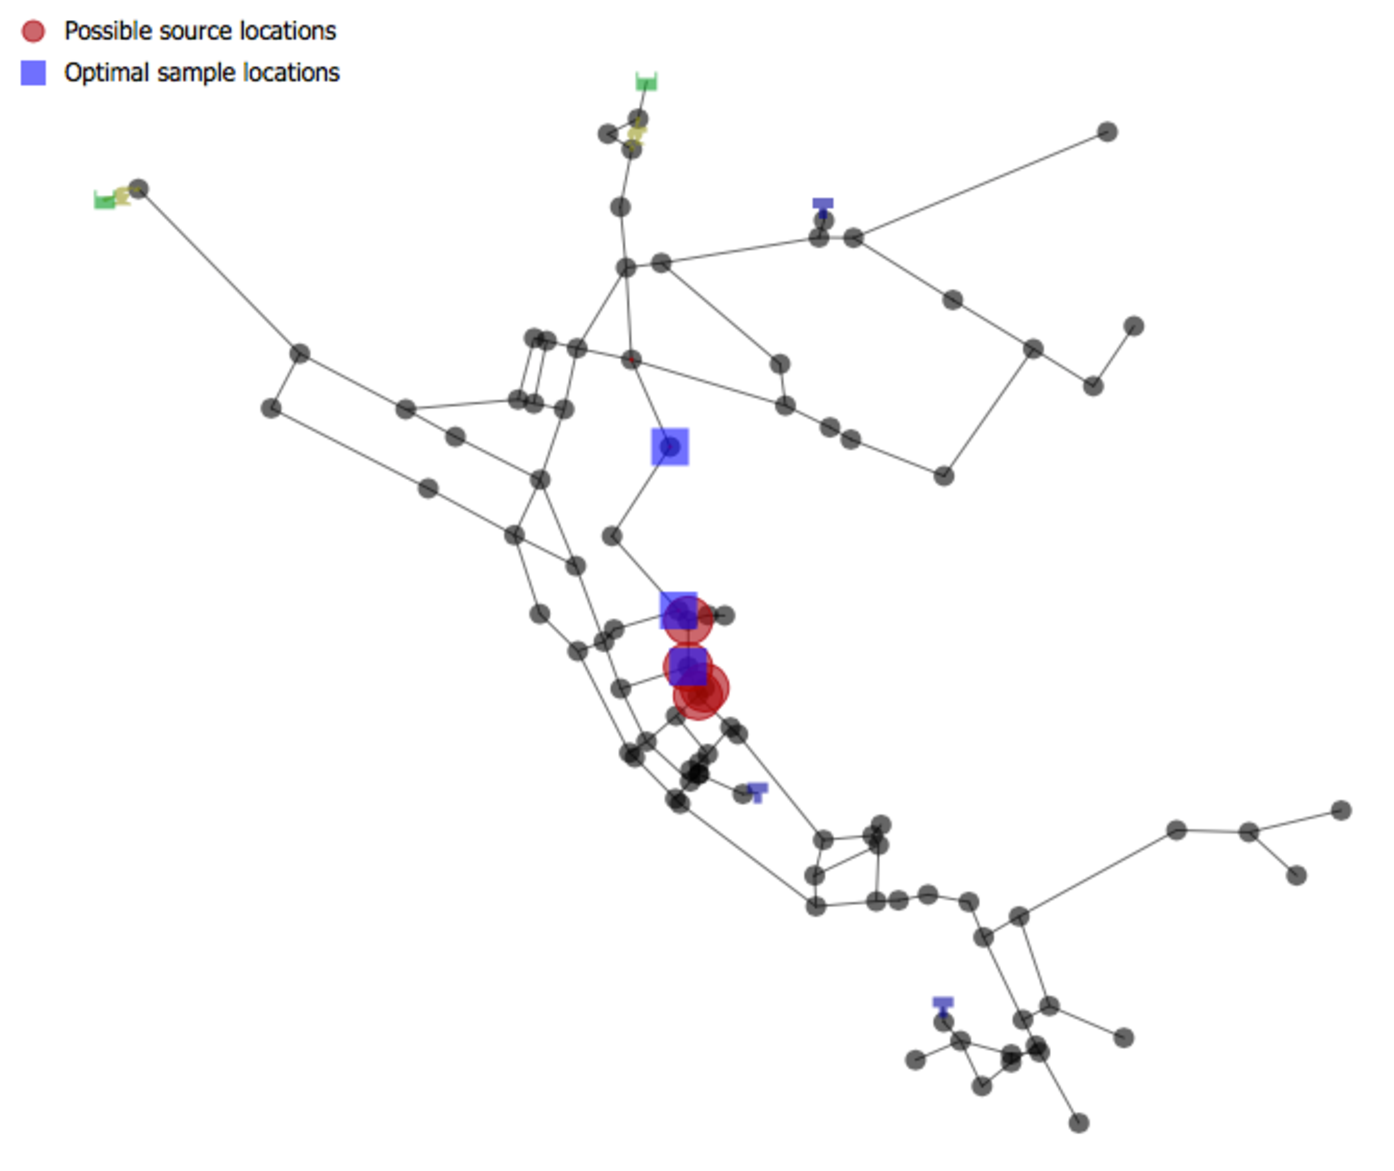
\includegraphics[scale=0.6]{graphics/inversion_cs_cycle2.pdf}
\caption{Cycle 2 identified optimal grab sample locations (blue).}
\label{fig:case_study_cycle2}
\end{center}
\end{figure}

The files required and generated during this cycle of source inversion and grab sample are 
provided in the \code{examples/case\_studies/inversion/Cycle2} folder.  
        
\subsection{Cycle 3}
Grab sample measurements are obtained at 9:30 AM from the optimal locations identified in Cycle 2. 
These along with the new measurements obtained from the fixed sensors are used to perform source inversion again. 
Only the seven possible injection nodes obtained in Cycle 2 are considered as feasible nodes in the \code{inversion} subcommand 
for Cycle 3. Three possible injection locations as shown in Figure \ref{fig:case_study_cycle3} are identified in this cycle.

\begin{figure}[!ht]
\begin{center}
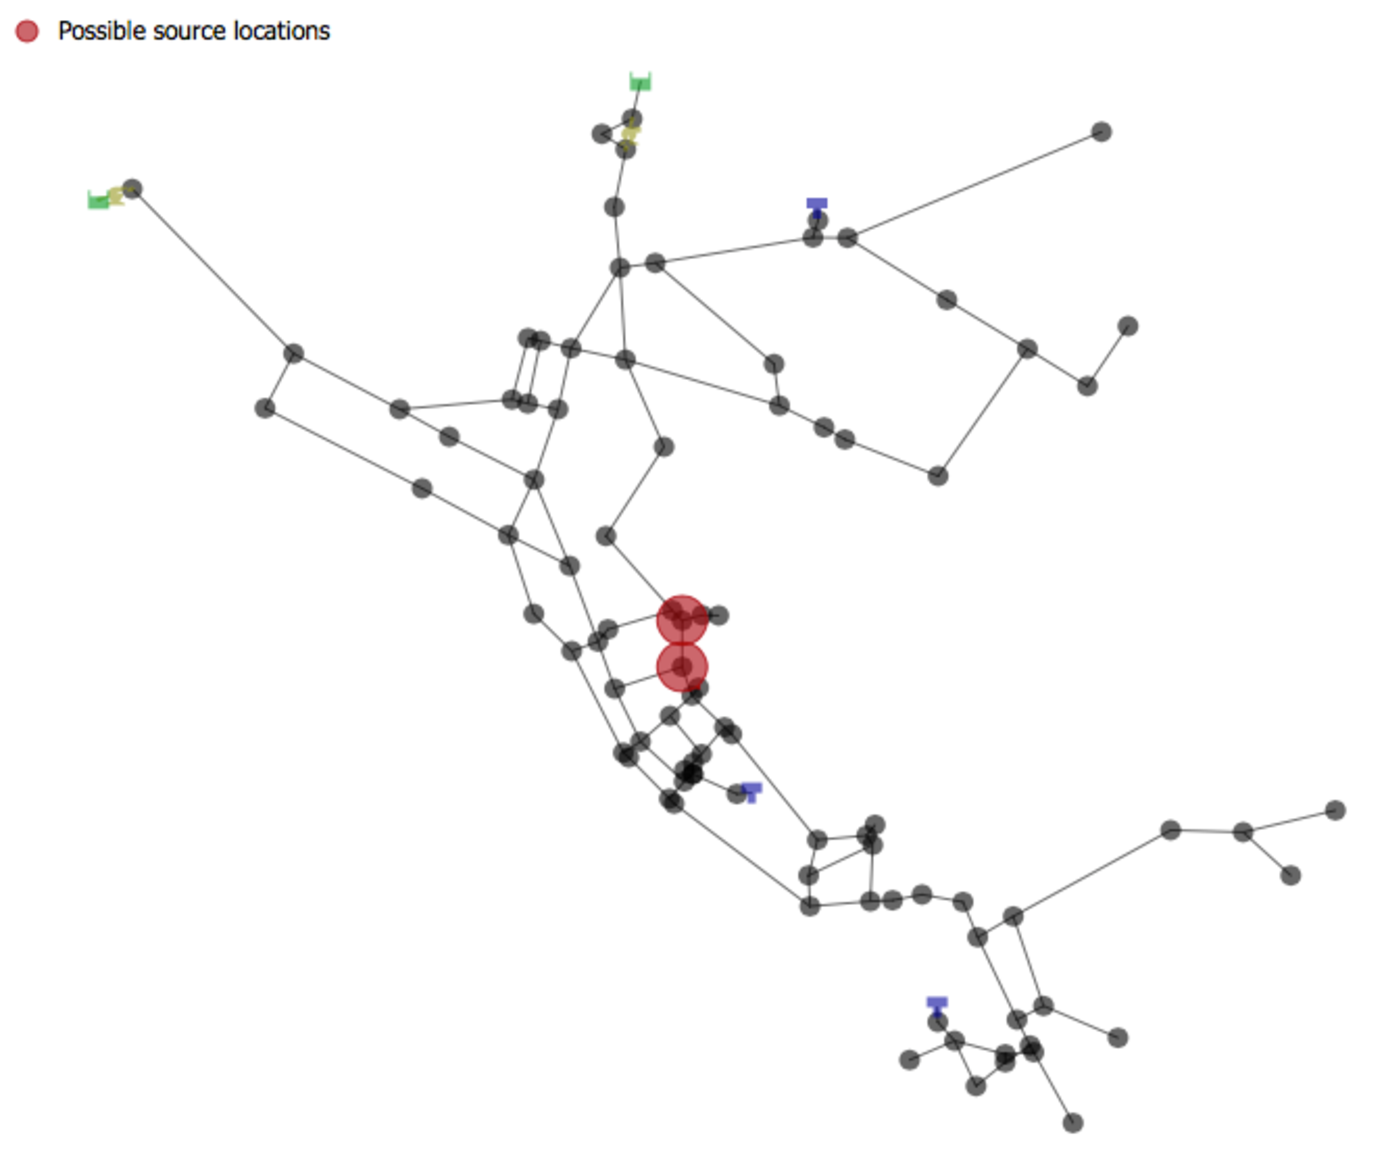
\includegraphics[scale=0.6]{graphics/inversion_cs_cycle3.pdf}
\caption{The possible injection nodes (red) identified in Cycle 3.}
\label{fig:case_study_cycle3}
\end{center}
\end{figure}

Since the water utility has three sampling teams available, the teams can directly inspect the three possible injection locations 
identified in this cycle to confirm the true injection location.  

\newpage

\section{Uncertainty Reduction with Grab Samples Case Study}\label{chap:samplingCase} 
\label{sampling_case_study}
The following case study illustrates how the functionality of the \code{inversion}, \code{grabsample} and \code{uq} subcommands 
can be used in tandem to identify multiple sampling cycles that reduce uncertainty in the extent of contamination.
The approach uses successive measurements obtained from manual grab samples to find the contamination plume.  
Figure \ref{fig:ureduction_flowchart} illustrates the methodology.
A contamination incident is first suspected following a customer inquiry or detection from a fixed continuous 
sensor in the Contamination Warning System (CWS). 
At this stage, a team is sent out to gather manual grab samples at and around the location of first detection. 
Discrete yes/no measurements from these manual grab samples along with the measurement from contamination warning system 
are then used to estimate the probability that nodes in the network are contaminated.
The probability of node contamination provides a metric of uncertainty quantification. Given a particular confidence level (e.g., 95\%), 
nodes can be categorized according to their probability of contamination: LY for ``likely yes,'' LN for ``likely no'' and UN for ``unknown.''  

If a sufficiently small number of nodes remain uncertain, then the process is terminated, otherwise further sampling cycles are required. 
This cycle of collecting manual grab samples is continued until the contamination plume is estimated with a good level of confidence. 
\begin{figure}[!ht]
\begin{center}
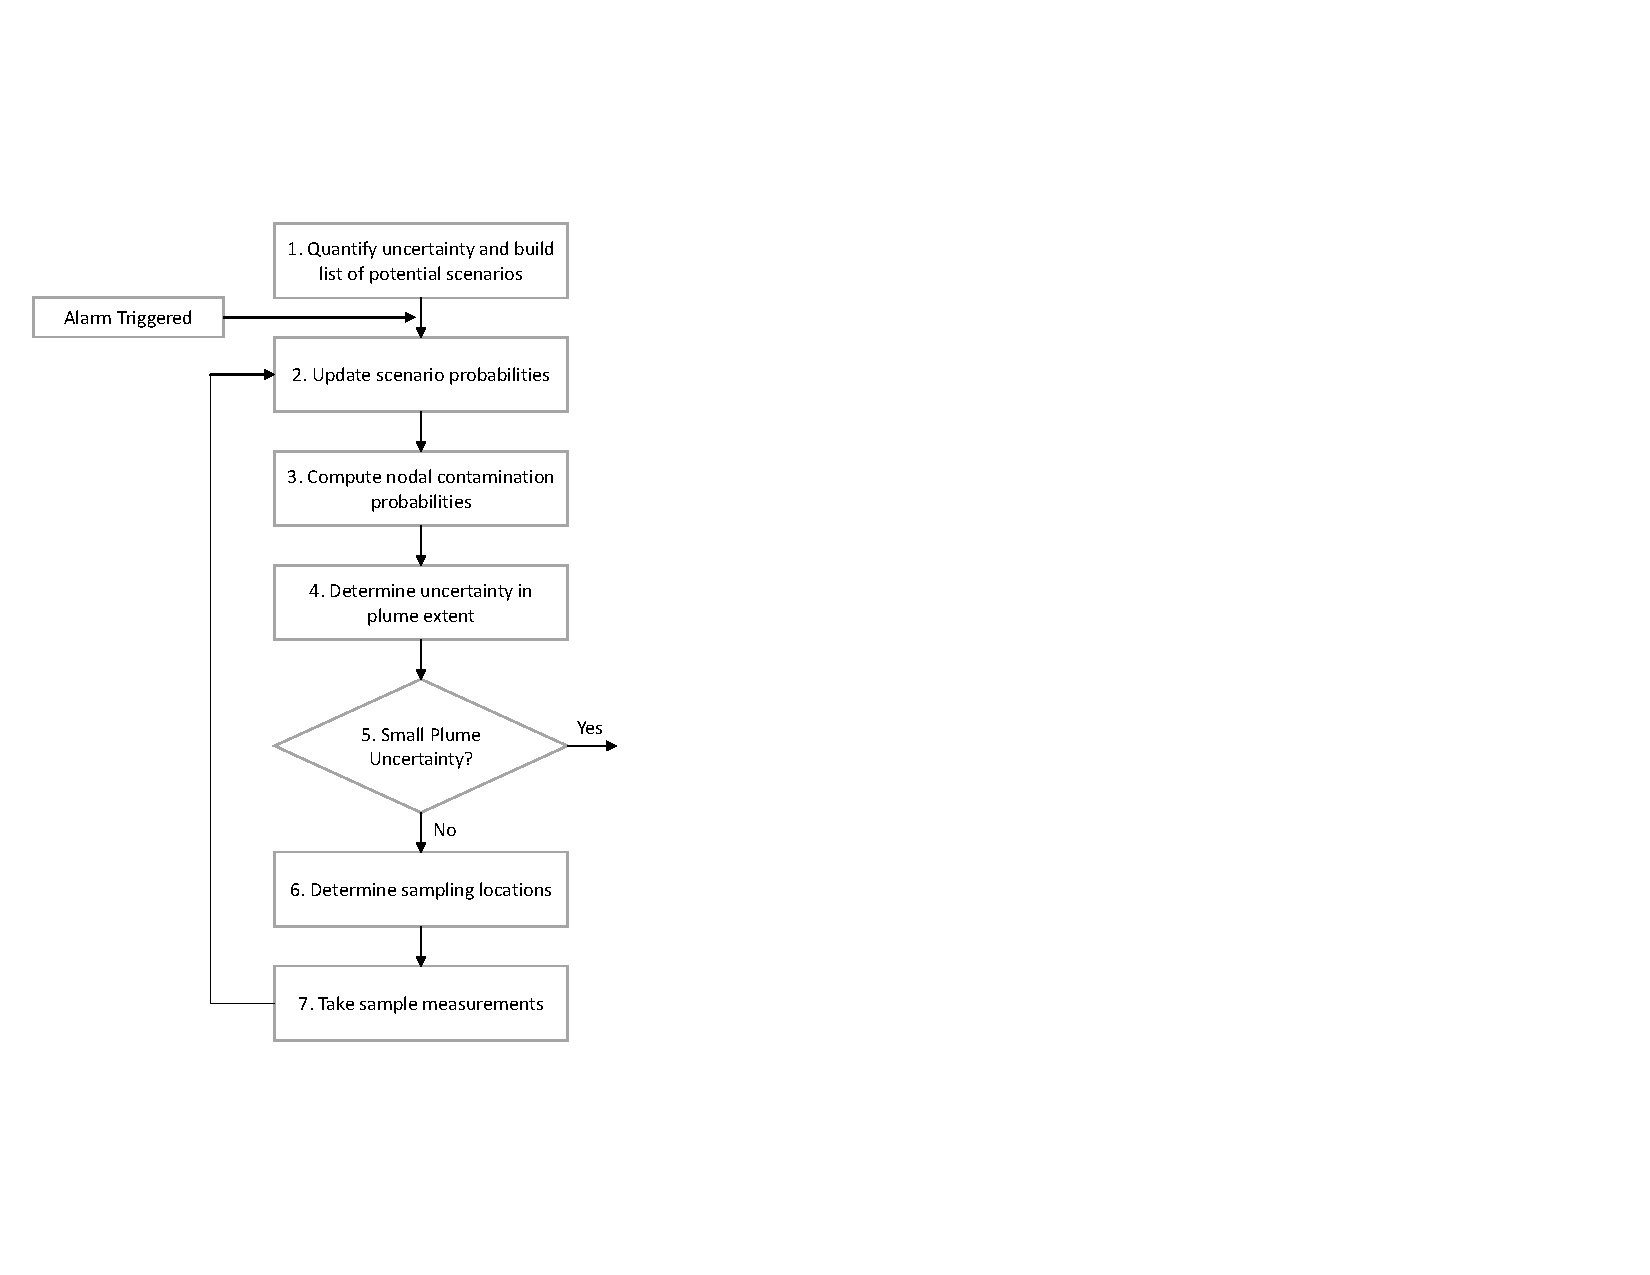
\includegraphics[scale=0.6]{graphics/uncertaintyprocess3.pdf}
\caption{Illustration of the source inversion and grab sample cycling strategy.}
\label{fig:ureduction_flowchart}
\end{center}
\end{figure}

\subsection{Case Study}
Since real system data is not available, the \code{measuregen}
executable is used again to generate simulated data for a contamination incident in the following case study.  In this simulation, 
a conservative contaminant is injected into node 115 of EPANET
Example Network 3 (Net3) at 8 am.  The set of potential scenarios includes 10 hydraulic realizations with 97 different injection locations. All of the files required 
for this case study are provided in the \code{examples/case\_studies/sampling} folder.
  
The case study is composed of four sampling cycles to reduce uncertainty in the extent of contamination. The initial warning is 
raised at 10 am. From this time, the procedure in Figure \ref{fig:ureduction_flowchart} is followed to reduce uncertainty by gathering 
grab samples every hour. In each sampling cycle, three additional samples are collected. Given the information provided by the new samples, 
the probability distribution of scenarios is updated following Bayesian statistics. Then, the methodology proposed in Section \ref{uqn_algorithms} 
is followed to quantify uncertainty. To facilitate the analysis, a script was implemented in Python to run the sampling cycles in a loop, which is the signals.py file provided in the \code{examples/case\_studies/sampling/cycling} folder. 
The execution of the script follows the same convention as the WST subcommands:

\begin{unknownListing}
python wst/packages/pywst/pywst/cycling/signals.py cycle <configfile>
\end{unknownListing}

The options for the script are the same as the options provided in the sections of the \code{inversion}, \code{uq} and \code{grabsample} subcommands. 
Some additional options to specify duration of each cycle and number of cycles are added. The configuration file for this case study, sampling\_case\_study.yml, 
is shown in Figure \ref{fig:case_study_conf}.  

\begin{figure}[!ht]
  \unknownInputListing{../../examples/case_studies/sampling/sampling_case_study.yml }{}{1}{13}
  \caption{The configuration file for sampling case study.}
  \label{fig:case_study_conf}
\end{figure}

\subsection{Cycle 0}
At 10 AM, the contamination warning system detects abnormal water quality at nodes 40 and 111. The measurement data from those two locations is used to 
perform a Bayesian update in the probability of scenarios. At this point, given the probability distribution of scenarios, 73 possible scenarios are 
identified as most likely. The uncertainty in the number of scenarios is evident in the uncertainty quantification as most of the nodes are deemed unknown (UN). 
Figure \ref{fig:case_study_cycle1} shows in yellow all locations that are considered uncertain to have contamination. 
The utility has three teams available to gather manual grab samples and it takes 60 minutes for each team to 
obtain the manual samples. The probability-based formulation in Chapter \ref{chap:grabsample} identifies the three optimal grab sample locations shown 
in dark gray/black in Figure \ref{fig:case_study_cycle1}.             

\subsection{Cycle 1}
At 11:00 AM, the new measurements are used to perform a Bayesian update and an uncertainty quantification. 
This time the number of uncertain nodes is reduced by half as shown in Figure \ref{fig:case_study_cycle2}. Nodes in red are likely to be contaminated (LY) and 
nodes in blue are likely to not be contaminated (LN). Again a 60-minute delay for sample collection and three sample teams were used in the probability-based 
formulation in Chapter \ref{chap:grabsample} to identify the optimal grab sample locations at 12:00 PM. The three new and three previous grab sample locations (dark gray/black) are shown in Figure \ref{fig:case_study_cycle2}.
        
\subsection{Cycle 2}
Grab sample measurements are obtained at 12:00 PM from the optimal locations identified in second cycle of the \code{grabsample} subcommand. 
These are used to perform Bayesian update and an uncertainty quantification again. 
Only seven nodes remain uncertain (UN) as to whether they are contaminated in this cycle. As the uncertainty is still not small enough, three more sampling locations are 
identified by solving the probability based formulation of Chapter \ref{chap:grabsample}. The three new grab sample locations plus the six previous (dark gray/black) are shown in 
Figure \ref{fig:case_study_cycle3}.

\subsection{Cycle 3}
Grab sample measurements are obtained at 1:00 PM from the optimal locations identified in in third cycle of the \code{grabsample} subcommand. 
With this new information, the Bayesian update and the uncertainty quantification lead to zero nodes classified as uncertain (all are likely yes or likely no). The three new grab sample locations plus the nine previous (dark gray/black) are shown in Figure \ref{fig:case_study_cycle4}. Only 11 grab sample locations are shown in this cycle since one of the locations was selected to be sampled twice, since different sampling times can provide different measurement data. 

\begin{figure}[!h]
\centering
\begin{subfigure}{0.49\textwidth}
\centering
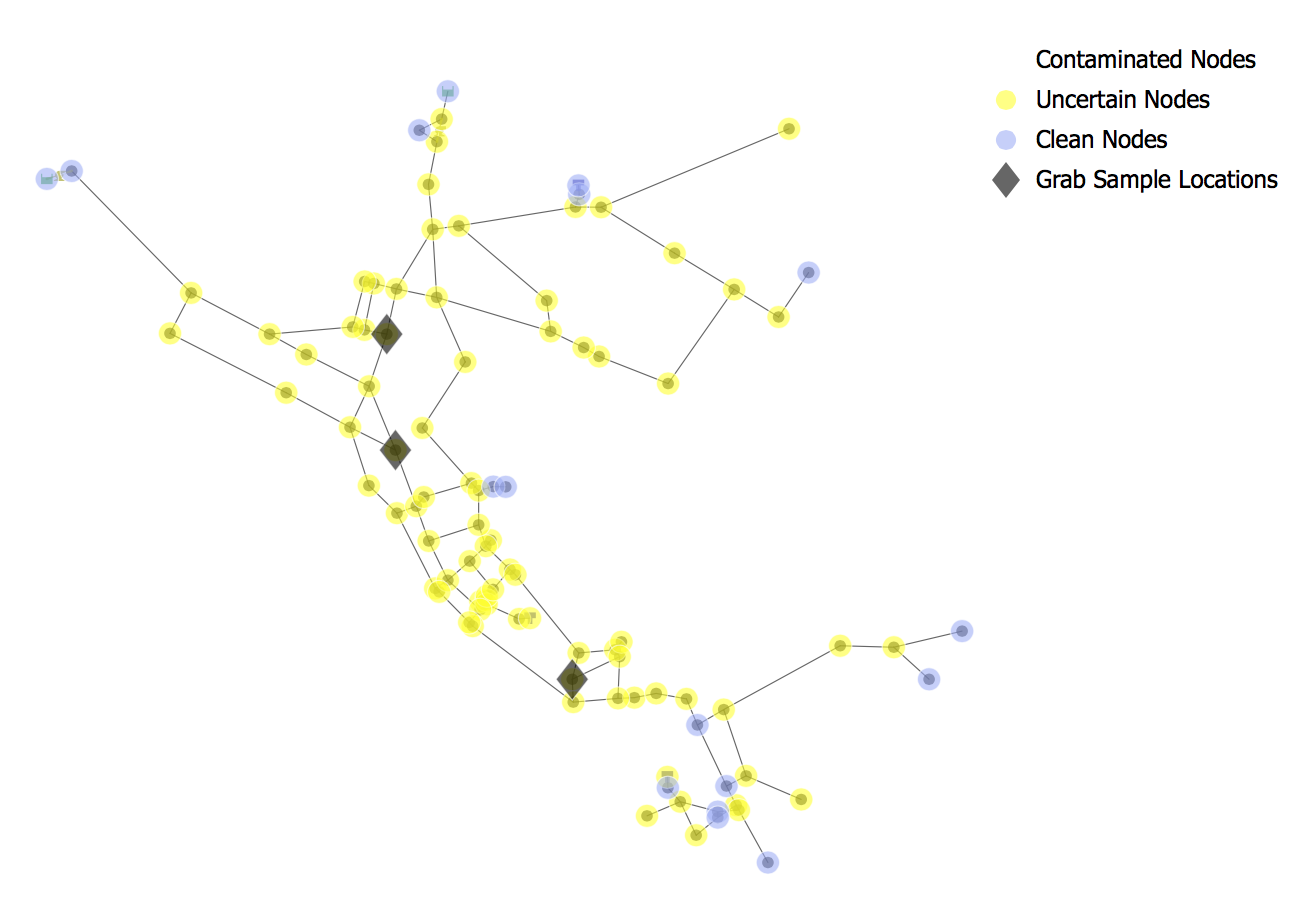
\includegraphics[width = \textwidth]{graphics/sampling_cs_cycle1.png}
\caption{Cycle 0}
\label{fig:case_study_cycle1}
\end{subfigure}
\begin{subfigure}{0.49\textwidth}
\centering
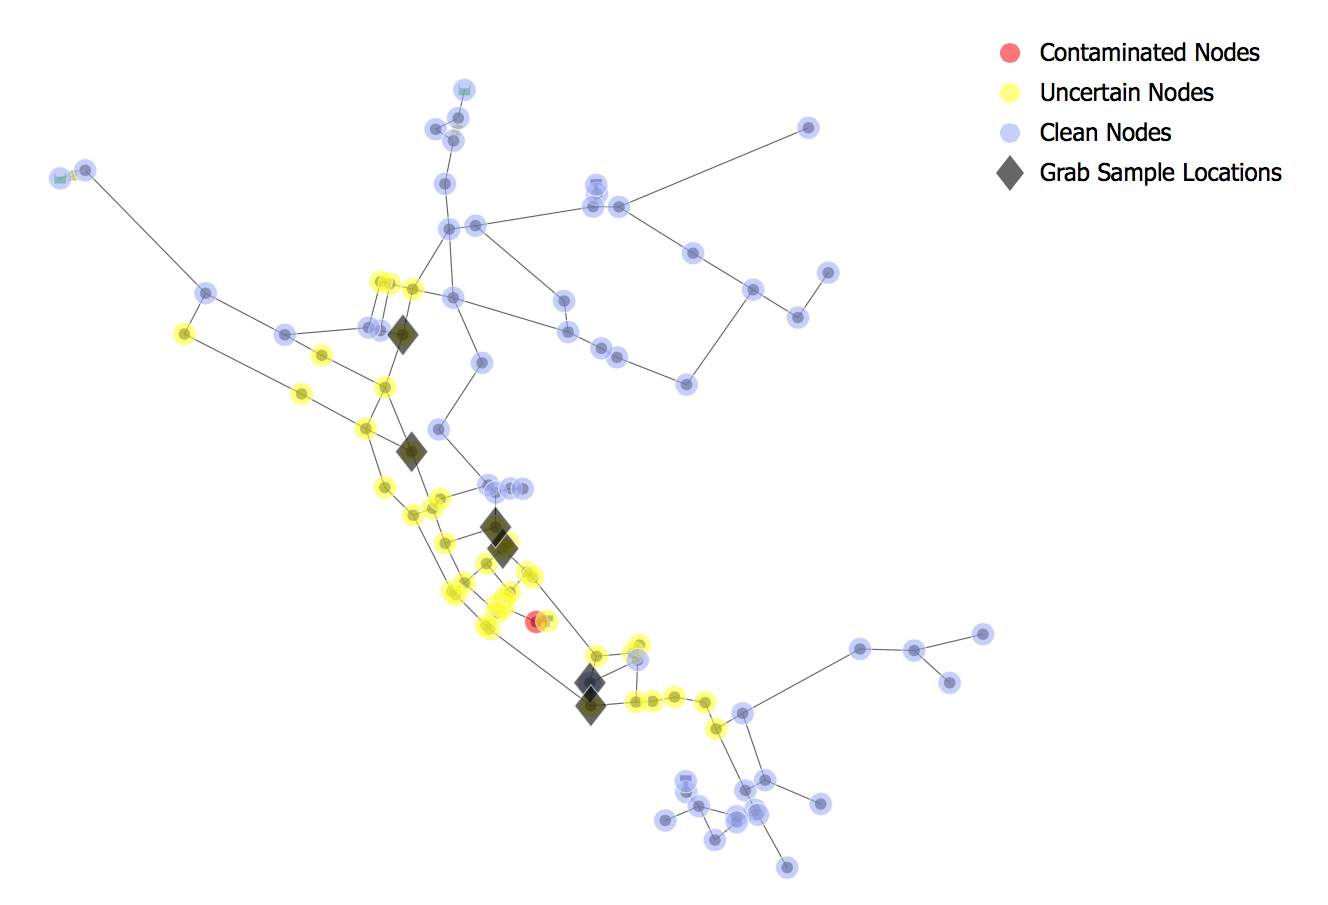
\includegraphics[width = \textwidth]{graphics/sampling_cs_cycle2.png}
\caption{Cycle 1}
\label{fig:case_study_cycle2}
\end{subfigure}
\centering
\begin{subfigure}{0.49\textwidth}
\centering
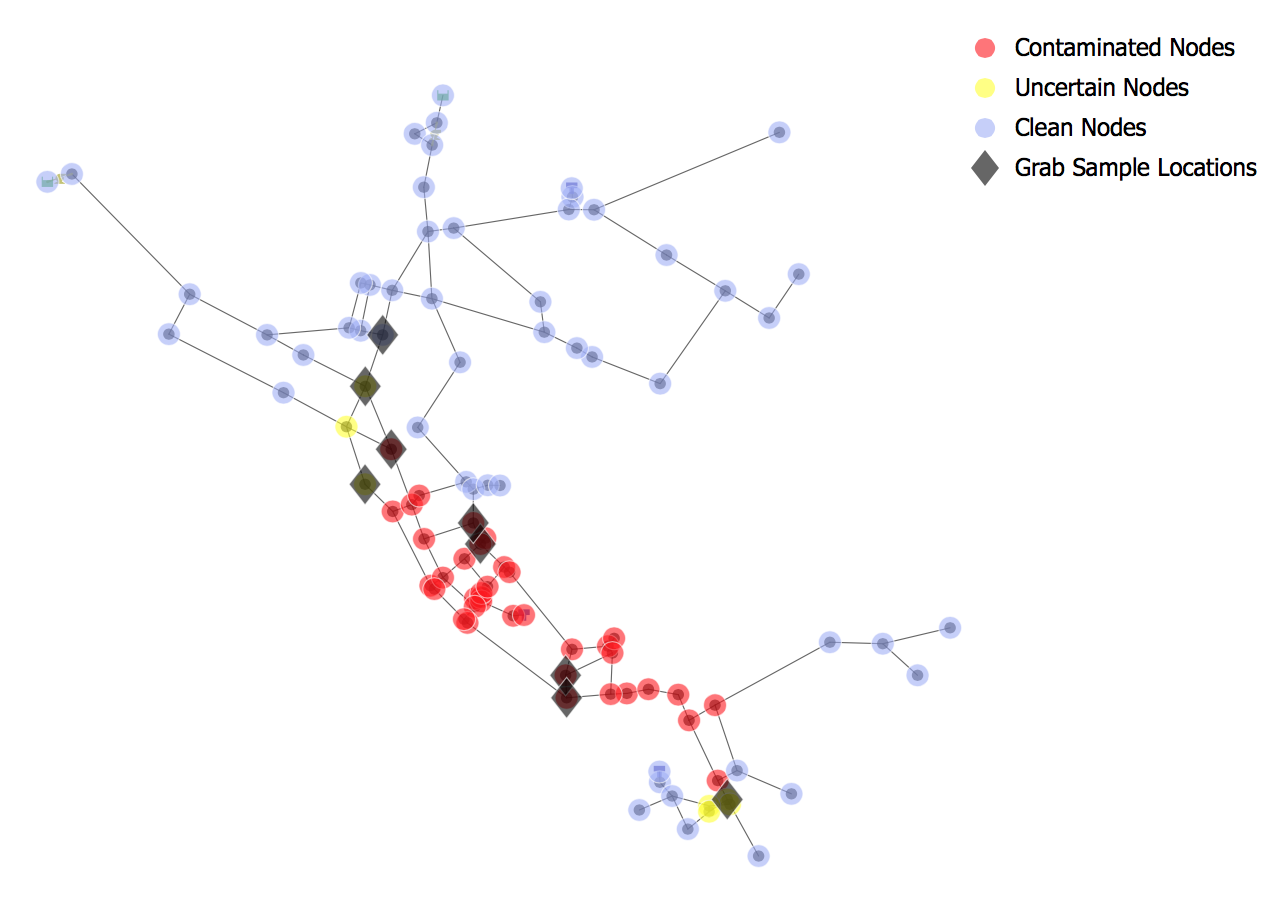
\includegraphics[width = \textwidth]{graphics/sampling_cs_cycle3.png}
\caption{Cycle 2}
\label{fig:case_study_cycle3}
\end{subfigure}
\begin{subfigure}{0.49\textwidth}
\centering
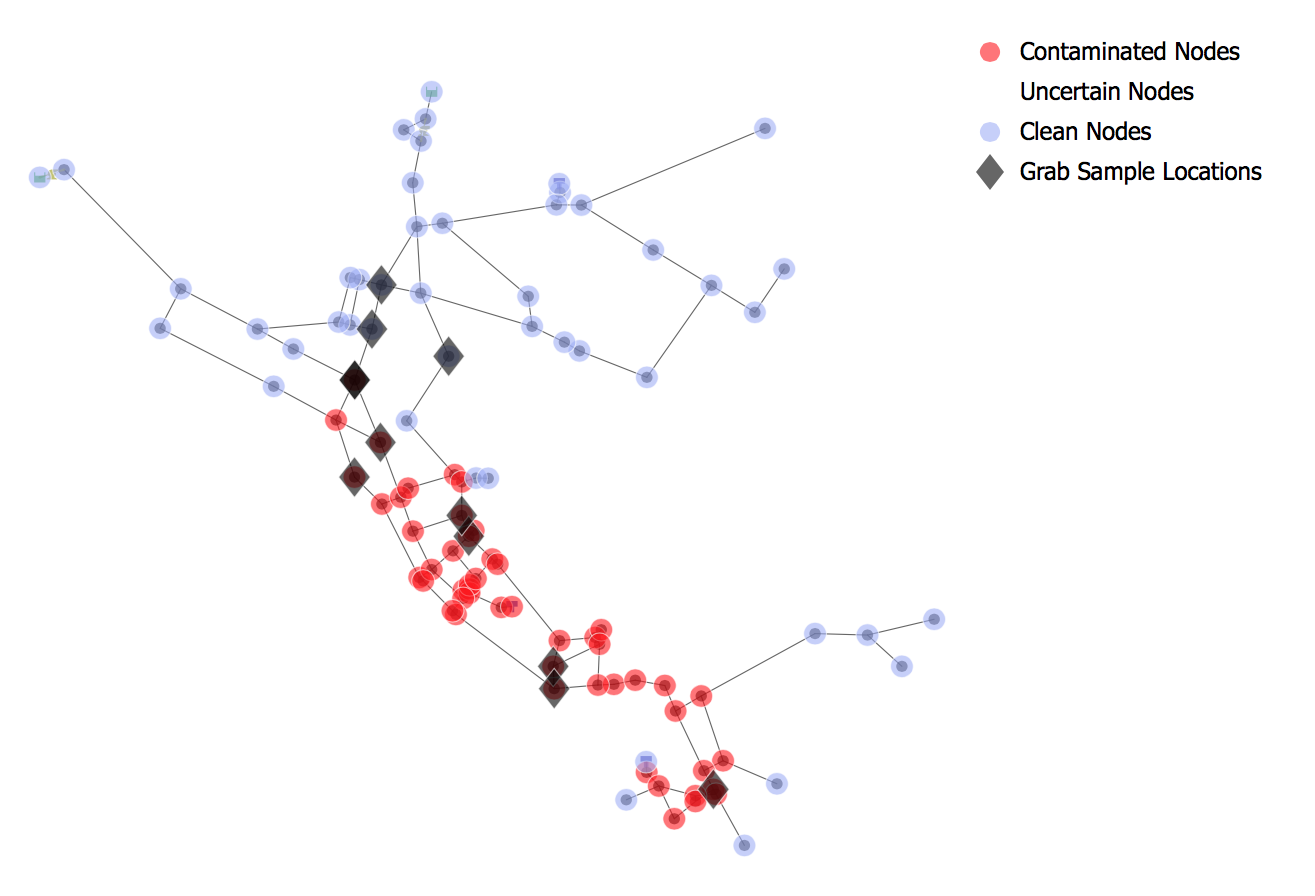
\includegraphics[width = \textwidth]{graphics/sampling_cs_cycle4.png}
\caption{Cycle 3}
\label{fig:case_study_cycle4}
\end{subfigure}
\caption{EPANET Example Network 3 with grab sample locations (dark gray/black diamonds), contaminated nodes (red circles), uncertain nodes (yellow circles), and clean nodes (blue-gray circles) identified for each of the cycles in the case study.}
\label{fig:gs_uq_case_study}
\end{figure}

\newpage

\newpage
\section{Flushing with Source Identification Case Study}\label{chap:flushCase} 
\label{flushing_case_study}
When a water utility becomes aware of a water quality issue either through 
customer complaints or water quality sensor alarms, they often open a hydrant to 
flush a portion of the distribution network in order to bring new water into the 
area and increase the chlorine residual. This case study examines how WST can 
be used to identify effective flushing locations following a water quality 
sensor alarm using the the \code{flushing}, \code{inversion} and 
\code{grabsample} subcommands. All files required to run the case study 
are provided in the \code{examples/case\_studies/flushing} folder.

The EPANET input file for this example is Net6.inp, which has a simulation duration 
of seven (7) days starting at midnight. The network is assumed to include a contamination 
warning system (CWS) with ten optimally placed water quality sensors and an 
event detection system in operation. The 10 sensors are located at 
JUNCTION-1617, JUNCTION-199, JUNCTION-2297, 
JUNCTION-2716, JUNCTION-2930, JUNCTION-3023, JUNCTION-435, JUNCTION-552, 
JUNCTION-675 and JUNCTION-831. The sensors were optimally placed 
using the \code{sp} subcommand. 
Figure \ref{fig:wds_sensors} shows the water distribution network and the location of the 
water quality sensors. The CWS provides binary values every 15 minutes from each sensor 
location. The binary value is zero if water quality conditions 
are normal or one if the conditions are abnormal.  

\begin{figure}[h!]
\begin{center}
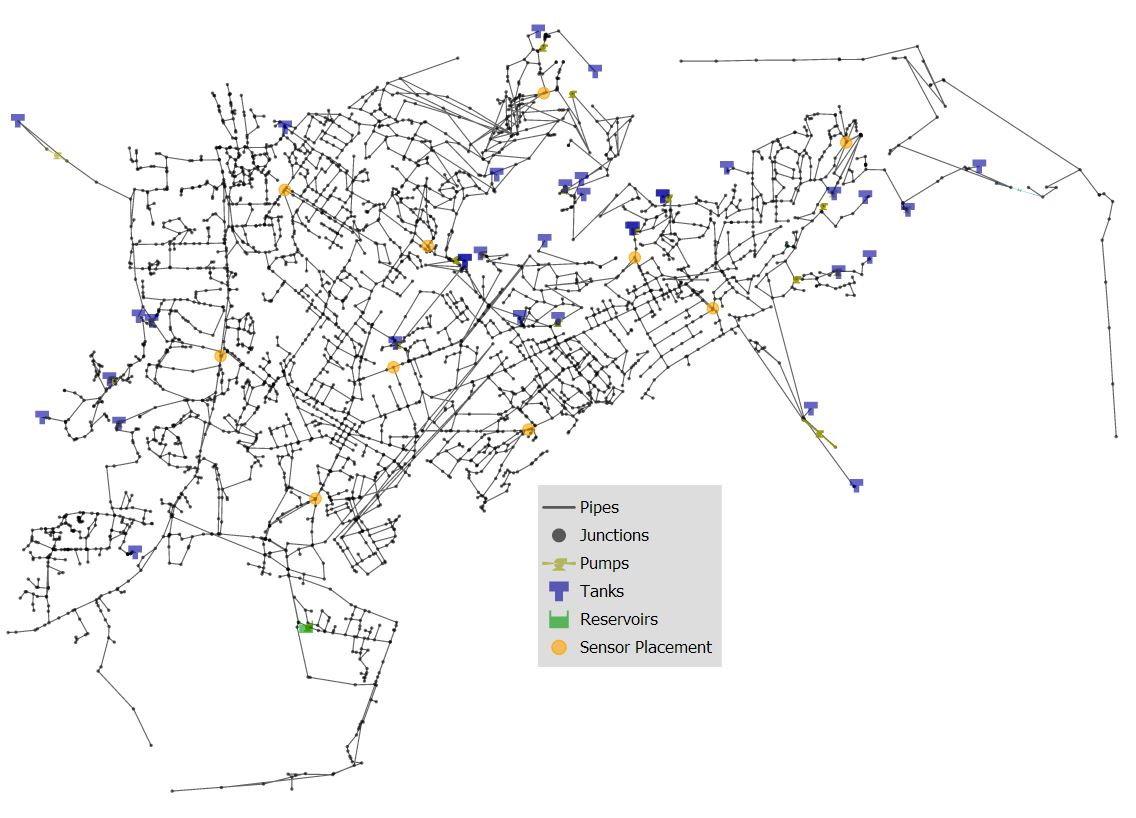
\includegraphics[scale=0.6]{graphics/Net6_Sensors.JPG}
\caption{Net6 water distribution network with water quality sensors.}
\label{fig:wds_sensors}
\end{center}
\end{figure}
 
At 10:15 AM, the CWS alerts water utility staff to abnormal water quality occurring 
at water quality sensor located at JUNCTION-1617 in water distribution network model. 
Figure \ref{fig:wds_sensors_detect} shows the JUNCTION-1617 highlighted as the sensor 
location with a positive detection of contamination in the network.  

\begin{figure}[h!]
\begin{center}
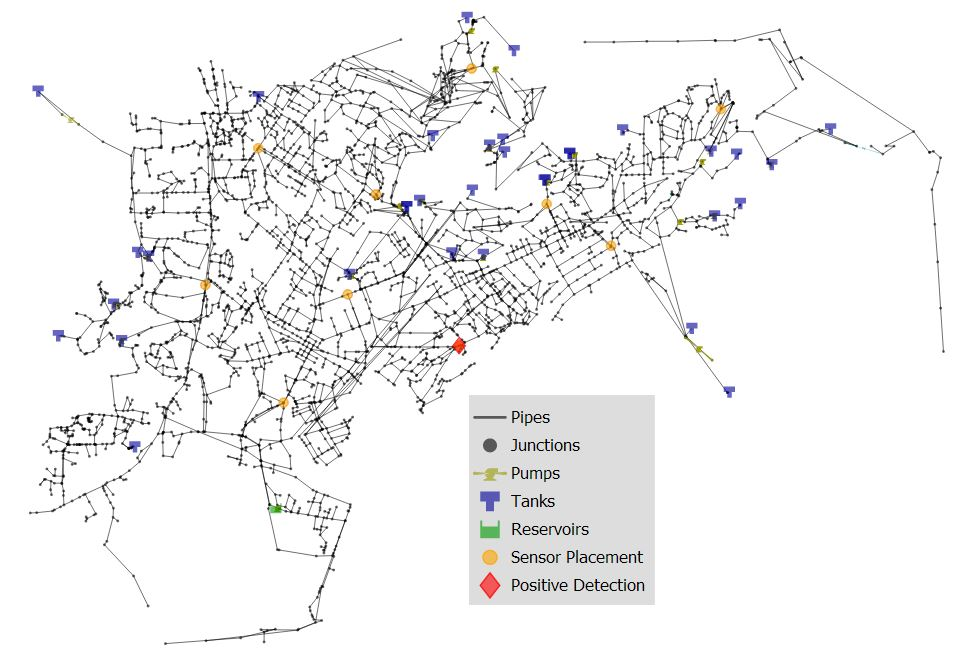
\includegraphics[scale=0.6]{graphics/Net6_Sensors_detect.JPG}
\caption{Net6 with positive contamination detection at JUNCTION-1617.}
\label{fig:wds_sensors_detect}
\end{center}
\end{figure}

The water utility must now decide how to proceed. The staff checks their 
consequence management plan and sends out a team to ensure that the water quality 
sensor is working properly. The water utility staff determines 
that a contamination incident is possible and they would like to identify the source.  
Source identification allows the water utility to determine the extent of contamination (or spread) and possibly
shut off any continuing injection of contaminants.  
Using the CWS information from the past 35 hours, provided in the measurements file 
Net6\_CWS\_MEASURES.dat, and the Net6 INP file, the \code{inversion} subcommand is used to 
identify the possible sources of the contamination. The inversion configuration file, 
Net6\_inversion.yml, and the measurements file are provided in the \code{examples/case\_studies/flushing} folder.

The \code{inversion} subcommand can be executed using the following command line:

\begin{unknownListing}
wst inversion Net6_inversion.yml
\end{unknownListing}  

Figure \ref{fig:wds_sources} shows the 25 possible contamination sources identified by the 
\code{inversion} subcommand.  

\begin{figure}[h!]
\begin{center}
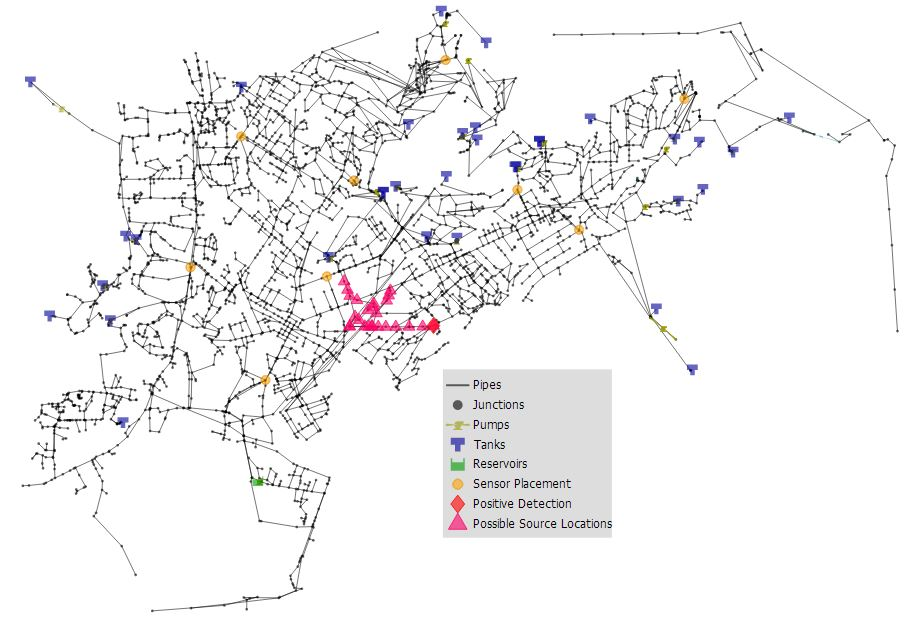
\includegraphics[scale=0.6]{graphics/Net6_possible_sources.JPG}
\caption{Net6 with possible contamination sources identified by \code{inversion} subcommand.}
\label{fig:wds_sources}
\end{center}
\end{figure}

Since flushing is a common response to abnormal water quality, the water utility staff decide 
to open hydrants to flush the contaminated water out of the network. To determine the most 
effective flushing locations, the staff simulates contamination incidents from each 
possible contamination source location using the TSG file produced from the \code{inversion} subcommand. 
From these simulations, the possible extent of contamination from each source location is identified. 
The nodes in the water distribution network model which are calculated to have 
contaminant concentrations above zero at the starting of flushing (12:00 PM, 
approximately two hours after detection) are considered as the initial starting points for the network 
solver option in the \code{flushing} subcommand. These initial starting points 
are the first node locations that are going to be evaluated in terms of the impact metric  
and then as the process continues, the solver will look at all of the nodes that are 
connected to these initial points to determine their impact metrics. Figure \ref{fig:wds_impacted_nodes} 
shows the nodes impacted by the 25 possible contamination source locations.  

\begin{figure}[h!]
\begin{center}
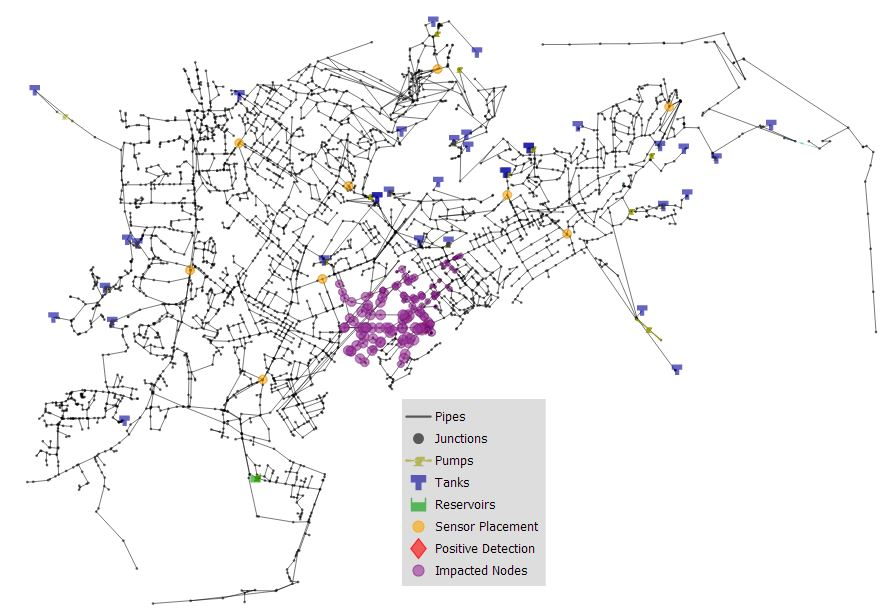
\includegraphics[scale=0.6]{graphics/Net6_imapcted_nodes_25inj.JPG}
\caption{Net6 with nodes impacted by the 25 possible contamination sources.}
\label{fig:wds_impacted_nodes}
\end{center}
\end{figure}

The water utility decides to open two hydrants to flush the contaminated water out of the network, 
since the extent of contamination for the possible 25 contamination sources (as seen in 
Figure \ref{fig:wds_impacted_nodes}) is not very large at the 
start of flushing at 12:00 PM. To identify effective 
flushing locations, the \code{flushing} subcommand is used. This command requires the following 
files as specified in the flushing configuration file, Net6\_flush\_2nodes.yml:

\begin{itemize}
\item Net6.inp - Net6 EPANET input (INP) file.
\item Net6\_inv1\_profile.tsg - The TSG file created by the \code{inversion} subcommand.
\item Net6\_bio.tai - The TAI file describing the dose-response characteristics for the assumed contaminant. 
This file is required when using the population exposed (PE) impact metric. 
\end{itemize}  

In addition, characteristics of the flushing response are also defined in the 
flushing configuration file. These include:

\begin{itemize}
\item A list of nodes that can be flushed - All non-zero demand (NZD) nodes 
\item The maximum number of nodes which can be flushed simultaneously - 2 
\item The flushing rate - 1100 gallons/min
\item The flushing duration - 8 hours 
\item The response time delay (time between detection and start of flushing) - 1 hour
\end{itemize}  

Other information provided in the flushing configuration file include the 
impact metric that is going to be minimized (PE), the nodes where water 
quality sensors are located, the type of solver (network solver), 
and the initial starting points for the network solver (JUNCTION-1881 and 
JUNCTION-1878). 

The \code{flushing} subcommand can be executed using the following command line:

\begin{unknownListing}
wst flushing Net6_flush_2nodes.yml
\end{unknownListing}  

Figure \ref{fig:wds_flushing_nodes} shows the flushing nodes identified by 
the \code{flushing} subcommand. The flushing nodes identified are JUNCTION-1881 
and JUNCTION-2233.  

\begin{figure}[h!]
\begin{center}
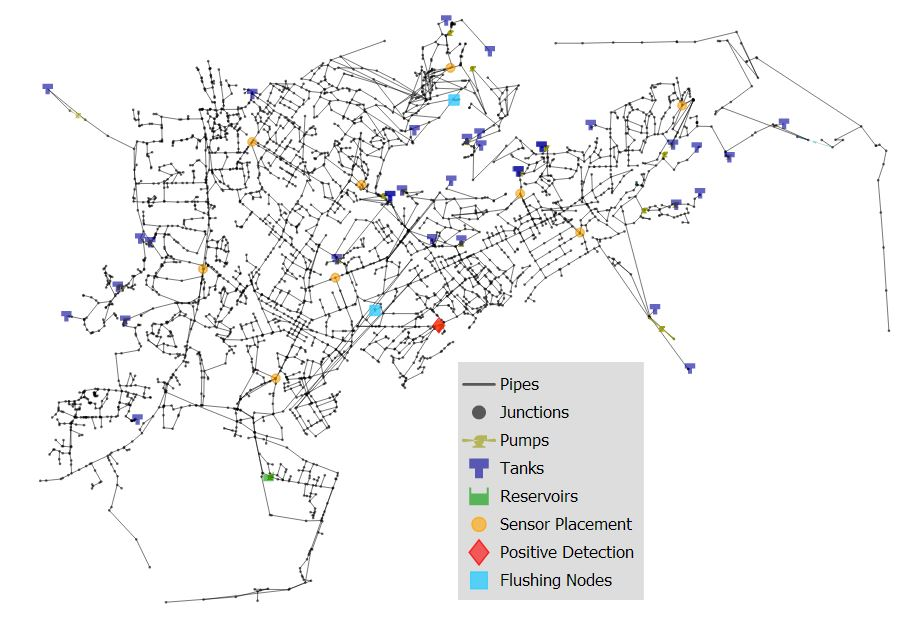
\includegraphics[scale=0.6]{graphics/Net6_2nodes_flushing.JPG}
\caption{Net6 with the flushing nodes identified by the \code{flushing} subcommand.}
\label{fig:wds_flushing_nodes}
\end{center}
\end{figure}

Since the identified flushing nodes were based upon the 25 possible contamination sources, 
the water utility staff evaluate the flushing response against each of the possible 
sources assuming it was the true source of the contamination. This option is available 
using EVALUATE as the type under the solver block of the flushing configuration file. An 
example flushing configuration file for the evaluate option is provided in 
Net6\_flush\_2nodes\_eval\_JUNC1617.yml in the \code{examples/case\_studies/flushing} folder. 
This example assumes that JUNCTION-1617 is the true source of contamination in the network 
and it evaluates the effectiveness of the identified flushing locations in terms of the 
PE metric. If JUNCTION-1617 is the true source, flushing at JUNCTION-1881 and JUNCTION-2233 
reduces the PE metric by only two percent (2\%).

% \todo{can you assume a different true source?  This one is among the worst.}

The \code{flushing} subcommand for this example can be executed using the following command line:

\begin{unknownListing}
wst flushing Net6_flush_2nodes_eval_JUNC1617.yml
\end{unknownListing}

Because the \code{inversion} subcommand solvers assume a continuous injection, the 
created TSG file has the contamination injection durations lasting as long as the 
simulation duration listed in the network INP file. Thus, the contamination injections 
start a little before the detection time and stop at the end of the simulation 
(seven days). Since an important response action would include shutting off the 
source of contamination, the TSG file is modified to stop the injection five 
hours after detection. Using the modified TSG file, the flushing response is evaluated 
against each of the 25 possible sources assuming it was the true source of the contamination.   
Figure \ref{fig:flushing_pe_reduction} shows the percent reduction in the PE metric 
for each of the 25 possible contamination sources with flushing alone (blue) and 
flushing with shutting off the contamination source (green). The percent 
reduction in the PE metric ranges from 24\% to 97\% for the flushing with source shut-off 
response action, which is an increase from the range of 2\% to 45\% for the flushing alone 
action. The highest percent reduction was if the true injection incident occurred at JUNCTION-1881.

\begin{figure}[h!]
\begin{center}
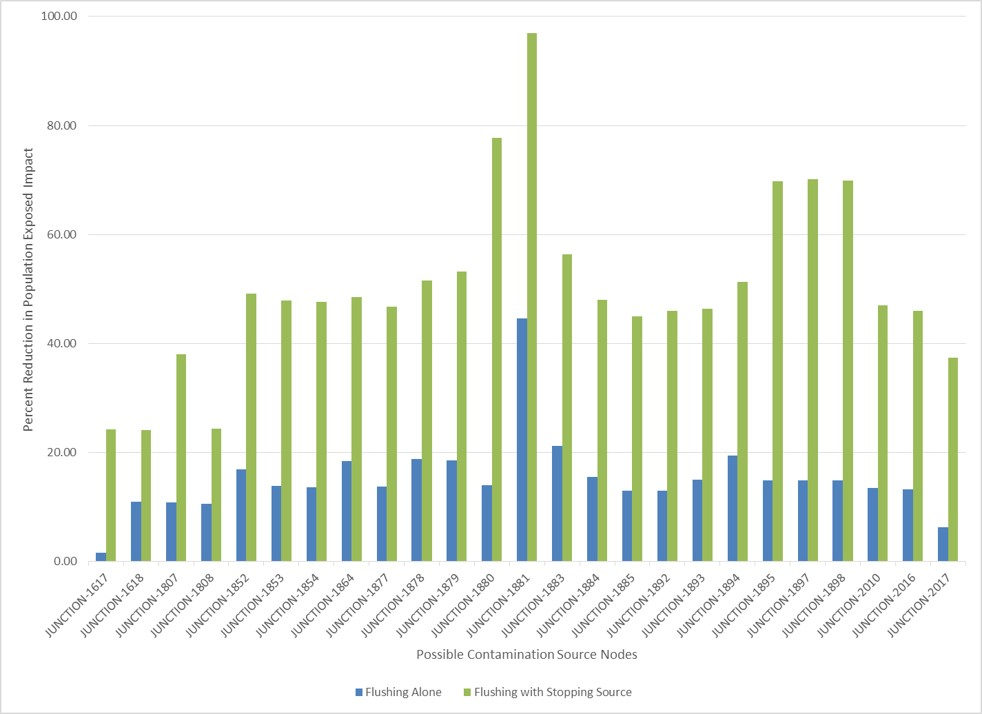
\includegraphics[scale=0.6]{graphics/flushing_pe_reduction.jpg}
\caption{The reduction in the PE metric for each of the 25 possible contamination sources.}
\label{fig:flushing_pe_reduction}
\end{center}
\end{figure}

% If the water utility wants to reduce the number of possible contamination sources 
% and improve the effectiveness of the flushing response, they could send staff to 
% manually collect grab samples to supplement the CWS measurements. 
 
% \todo{was grabsample used?}

\newpage

  
  \chapter{File Formats}
  \label{fileFormats} 
  This chapter describes the different file formats used by WST, including a 
brief description, format, the associated subcommand(s) and any additional details.

\section{Configuration File}\label{formats_yamlFile}
\begin{itemize}
\item {\bfseries Description:} Input configuration file for all WST subcommands.
\item {\bfseries Format:} YAML 
\item {\bfseries Created by:} Template input configuration files can be created using the \code{---template} option from each subcommand in WST.
\item {\bfseries Used by:} WST
\item {\bfseries Details:} 
The input configuration files for WST are stored in the YAML file format.
YAML is a human-readable file format that is well suited for storing hierarchical 
information. This information can be easily parsed and stored as common data types 
such as strings, scalars, lists and dictionaries by a range of programming languages. 
WST uses PyYAML to parse YAML files into Python data types. Basic YAML format specifications are listed below:
\begin{itemize}
\item Each element of a YAML file is a key, value pair separated by a colon (key:value).  
\item The key is the name given to the element, and the value is the data for that element.  
\item The hierarchy of YAML files is maintained by outline indentation. 
\item The number of spaces used to indent an element in the YAML file must be consistent across all elements at the same hierarchical level.  
\item Nested data elements must be indented further than their preceding level.
\item Using tab for indentation is not recommended.
\item Optional blank lines can be added for readability. 
\item Comments begin with the number sign (\#) and must be separated from a key:value 
pair by space. Comments can start anywhere but are limited to a single line.
\item PyYAML automatically casts data types. For example, [123] is read as a list 
with a single integer value, '123' is read as a string, 123 is read as an integer, and 123.0 is read as a real number.
\item Strings do not require quotation (unless they could be cast as a number) and can contain spaces.
\item Lists are indicated with square brackets or hyphens. When using square brackets, the list is comma separated. When using hyphens, each entry of the list is on a new line.
\item Dictionaries are indicated with indentation or curly brackets and are used to define key: value pairs.  Nested dictionaries define the hierarchical levels in the YAML file.
\end{itemize}
Additional information on YAML files can be found on the official YAML website \url{http://www.yaml.org}.

Select aspects of the \code{flushing} subcommand template configuration file are used as an example of the format of a YAML file. 
The full \code{flushing} subcommand template configuration file is shown in Figure \ref{fig:flushing_template}. 
In the template, the top level key, denoted 'flushing', contains the following data:
\unknownInputListing{examples/flushing_config.yml}{}{1}{50}
This subset of the the \code{flushing} subcommand template is refereed to as the flushing block. Instead of a single 
value assigned to 'flushing', the value is a dictionary containing a nested structure 
of additional key:value pairs. 

The keys 'detection', 'flush nodes' and 'close valves' are all second level keys inside the flushing block. 
The location of these keys is often specified using the notation [flushing][detection], [flushing][flush nodes] and [flushing][close valves]. 
The second level keys must be indented using the same number of spaces and they must have unique names. 
The key [flushing][detection] is assigned to a list. Lists can be specified 
in one of two ways, using square brackets or using hyphen. The following two formats (separated by -\--\--) are equivalent. 
\begin{unknownListing}
flushing:
  detection: [111, 127, 179] # square bracket notation, comma separated
---
flushing:
  detection: # hyphen notation, new line for each entry
  - 111
  - 127
  - 179
\end{unknownListing}
All template configuration files use square brackets to indicate where a list of input values can be used.
If these input values include keywords, like NZD for non-zero demand nodes, this 
information is listed in the comment or in the user manual documentation for 
that specific YAML input parameter.

The options [flushing][flush nodes] and [flushing][close valves] are both assigned dictionaries. 
The data inside these second level keys contain additional key:value pairs. 
All keys within these dictionaries must be indented using the same number of spaces and have unique names. 
Two key:value pairs in the flushing flush nodes option are listed below:
\begin{unknownListing}
flushing:
  flush nodes:
    feasible nodes: NZD
    max nodes: 2
\end{unknownListing}    
Here, the [flushing][flush nodes][feasible nodes] option is set to the string NZD 
and the [flushing][flush nodes][max nodes] option is set to the integer 2. 
Note that there are two third-order keys named 'response time', however they do not share the same exact hierarchy, as shown below:
\begin{unknownListing}
flushing:
  flush nodes:
    response time: 0.0
  close valves:
    response time: 0.0    
\end{unknownListing}    

YAML files can be written in a compact format that uses curly brackets to represent the hierarchical indentation of the nested dictonary. 
While this avoids issues with space indentation, this format is more difficult for the user to read. 
For example, the following two examples (separated by -\--\--) are equivalent: 
\begin{unknownListing} 
flushing:
  detection: [111, 127, 179] 
---
{'flushing': {'detection': [111, 127, 179]}}
\end{unknownListing}  
\end{itemize}

\section{Cost File}\label{formats_costFile}
\begin{itemize}
\item {\bfseries Description:} Specifies the costs for installing sensors at 
different nodes throughout a network. This is the cost of installing one sensor 
at one particular node. 
\item {\bfseries Format:} ASCII 
\item {\bfseries Created by:} WST user 
\item {\bfseries Used by:} \code{sp} 
\item {\bfseries Details:} Each line of this file has the format:
\begin{unknownListing}
   <EPANET node ID> <cost>
\end{unknownListing}
Nodes not explicitly enumerated in this file are assumed to have a cost of zero 
unless the ID \code{\_\_}default is specified. For example to specify that 
all un-\/enumerated nodes have a cost of 1.0:
\begin{unknownListing}
   __default 1.0
\end{unknownListing}

For example, the following cost file indicates that a sensor at node 1 has a cost of \$100, a sensor at node 2 has a cost of \$200 and sensors at all other nodes have a cost of \$50.
\begin{unknownListing}
     1       100
     2       200
   __default 50
\end{unknownListing}
\end{itemize}

\if 0
\section{DVF File}\label{formats_dvfFile} 
\begin{itemize} 
\item {\bfseries Description:} Provides representation of flushing variables (opened hydrants and closed pipes).
\item {\bfseries Format:} ASCII 
\item {\bfseries Created by:} WST user or \code{flushing}
\item {\bfseries Used by:} \code{tevasim} and \code{sim2Impact}
\item {\bfseries Details:}
\unknownInputListing{fileFormats/dvfFormat.txt}{}{1}{16}{}
\end{itemize} 
\fi

\section{ERD File}\label{formats_tsoFile} 
\begin{itemize} 
\item {\bfseries Description:} Provides a compact representation of all contamination scenario simulation results. 
\item {\bfseries Format:} binary 
\item {\bfseries Created by:} \code{tevasim} 
\item {\bfseries Used by:} \code{sim2Impact} 
\item {\bfseries Details:} The simulation data generator produces four output files 
containing the results of all contamination simulation scenarios.  The database files include 
an index file (index.erd), a hydraulics file (hyd.erd) and a water quality file (qual.erd).  
The files are unformatted binary file in order to save disk space and computation time. 
They are not readable using an ordinary text editor.  
%All data written are either of type float, int, long, or 16-byte character strings. The format of this file is as follows. 
%\unknownInputListing{fileFormats/tsoFormat.txt}{}{}
\item {\bfseries Note:} The ERD file format replaced the TSO and SDX file formats, created by previous versions of 
\code{tevasim}, to extend the capability of \code{tevasim} for multi-species simulation using EPANET-MSX.  
While the \code{tevasim} subcommand produces only ERD files 
(even for single species simulation), the \code{sim2Impact} subcommand accepts both ERD and TSO file formats. 
\end{itemize} 


\section{Impact File}\label{formats_impactFile}
\begin{itemize}
\item {\bfseries Description:} For each contamination scenario, the impact file 
contains a list of all the locations (nodes) in the network where a sensor might 
detect contamination from a specific scenario.
\item {\bfseries Format:} ASCII 
\item {\bfseries Created by:} \code{sim2Impact} 
\item {\bfseries Used by:} \code{sp} and \code{evalsensor} 
\item {\bfseries Details:} The first line of an impact file 
contains the number of incidents. The second line specifies the number of delays (always 1) and the delay time in minutes.
Subsequent lines have the format
\begin{unknownListing}
   <scenario-index> <node-index> <time-of-detection> <impact-value>
\end{unknownListing}
The scenario index is the index of contamination scenarios that were simulated. 
A scenario index maps to a line in the network scenariomap file, which is defined in Section \ref{formats_scenarioFile}. 
The node index is the index of a witness location for the incident. A node index maps to a line 
in the network nodemap file, which is defined in Section \ref{formats_nodeFile}. The time of detection is in minutes. 
The value of the impacts are in the corresponding units for each impact metric. The different 
impact metrics in each line correspond to the different delays that have been computed. 
\end{itemize}


\section{Imperfect Junction Class File}\label{formats_junctionClass}
\begin{itemize}
\item {\bfseries Description:} Provides the mapping from EPANET node IDs to failure classes of different false-negative probabilities. 
\item {\bfseries Format:} ASCII 
\item {\bfseries Created by:} WST user 
\item {\bfseries Used by:} \code{sp} 
\item {\bfseries Details:} The imperfect junction class file provides the mapping from EPANET node IDs
 to failure classes of different false-negative probabilities as defined in a imperfect sensor class file 
 (See Section \ref{formats_sensorClass} for information on imperfect sensor class files). The format of this file is:
\begin{unknownListing}
   <node id> <failure class>
   <node id> <failure class>
   ....
\end{unknownListing}

For example, node 1 is of class 2, node 2 is of class 1 and node 3 is of class 1:
\begin{unknownListing}
   1 2
   2 1
   3 1
   ....
\end{unknownListing}
\end{itemize}

\section{Imperfect Sensor Class File}\label{formats_sensorClass}
\begin{itemize}
\item {\bfseries Description:} Contains false-negative probabilities for different types of sensors. 
The false-negative probability defines the accuracy rate of the sensor (e.g., 50 percent of the 
time the sensor is providing a correct reading). 
\item {\bfseries Format:} ASCII 
\item {\bfseries Created by:} WST user 
\item {\bfseries Used by:} \code{sp} 
\item {\bfseries Details:} The file has format:
\begin{unknownListing}
   <class id> <false-negative probability>
   <class id> <false-negative probability>
   ....
\end{unknownListing}

For example, the following file defines a failure class 1 with a false-negative probability of 25 percent, 
and a failure class 2 with a false-negative probability of 50 percent:
\begin{unknownListing}
   1 0.25
   2 0.5
   ....
\end{unknownListing}
\end{itemize}

\section{Measurements File}\label{formats_measFile}
\begin{itemize}
\item {\bfseries Description:} Contains a list of measurements along with their corresponding time and EPANET node ID.
  This file can contain multiple node IDs and the measurement time is not required to be in order. 
\item {\bfseries Format:} ASCII
\item {\bfseries Created by:} WST user or a water quality event detection system or a data acquisition system  
\item {\bfseries Used by:} \code{inversion} 
\item {\bfseries Details:} Each line of this file has the format:
\begin{unknownListing}
   <EPANET node ID> <Time from beginning of simulation (sec) > <Binary yes/no measurement>
\end{unknownListing}
An example measurements file is provided:
\unknownInputListingFixed{../../examples/Net3/Net3_MEASURES.dat}{}{1}{10}
\end{itemize}

\section{Nodemap File}\label{formats_nodeFile}
\begin{itemize}
\item {\bfseries Description:} Provides a mapping from the indices used for sensor placement to the node IDs used within EPANET.
\item {\bfseries Format:} ASCII 
\item {\bfseries Created by:} \code{sim2Impact} 
\item {\bfseries Used by:} \code{evalsensor} and \code{sp} 
\item {\bfseries Details:} Each line of this file has the format:
\begin{unknownListing}
   <node-index> <EPANET node ID>
\end{unknownListing}
This mapping is generated by the \code{sim2Impact} subcommand, and all sensor placement solvers subsequently use the node indices internally. 
\end{itemize}


\section{Scenariomap File}\label{formats_scenarioFile}
\begin{itemize}
\item {\bfseries Description:} The scenariomap file provides auxiliary information about each contamination incident. 
\item {\bfseries Format:} ASCII 
\item {\bfseries Created by:} \code{sim2Impact} 
\item {\bfseries Used by:} \code{evalsensor} 
\item {\bfseries Details:} Each line of this file has the format:
\begin{unknownListing}
   <node-index> <EPANET node ID> <source-type> <source-start-time> ...
			<source-stop-time> <source-strength>
\end{unknownListing}
The node index maps to the network nodemap file as described in Section \ref{formats_nodeFile}, and the EPANET node ID provides 
this information. The source type is the injection mode for an scenario, e.g., 
flow-\/paced or fixed-\/concentration. The scenario source start and stop times are in minutes, and these values are relative to the 
start of the EPANET simulation. The source strength is the concentration of contaminant at the injection source. 
\end{itemize}


\section{Sensor Placement File}\label{formats_sensorPlacementFile}
\begin{itemize}
\item {\bfseries Description:} Describes one or more sensor placements. 
\item {\bfseries Format:} ASCII 
\item {\bfseries Created By:} \code{sp} 
\item {\bfseries Used By:} \code{evalsensor} 
\item {\bfseries Details:} Lines in a sensor placement file that begin with 
the \# character are assumed to be comments. Otherwise, lines of this file have the format
\begin{unknownListing}
   <sp-id> <number-of-sensors> <node-index-1> ...
\end{unknownListing}
The sensor placement ID is used to identify sensor placements in the file. Sensor 
placements could have differing numbers of sensors, so each line contains this 
information. The node indices map to values in the nodemap file described in Section \ref{formats_nodeFile}. 
\end{itemize}

\section{TAI File}\label{formats_taiFile}
\begin{itemize}
\item {\bfseries Description:} Describes the information needed for assessing health impacts.
\item {\bfseries Format:} ASCII 
\item {\bfseries Created by:} WST user 
\item {\bfseries Used by:} \code{sim2Impact} 
\item {\bfseries Details:} This file is required for health impact metrics, such as population exposed, population 
dosed and population killed. 
The following example can be copied directly into a text editor. 
\unknownInputListing{fileFormats/tiaFormat.txt}{1}{1}{102}
\end{itemize}


\section{TSG File}\label{formats_tsgFile}
\begin{itemize}
\item {\bfseries Description:} Specifies how an ensemble of EPANET 2.00.12 contamination scenario simulations will be performed. 
\item {\bfseries Format:} ASCII 
\item {\bfseries Created by:} WST user 
\item {\bfseries Used by:} \code{tevasim} 
\item {\bfseries Details:} Each line of a TSG file specifies injection location(s), species (optional), 
injection mass and the injection time-\/frame:
\begin{unknownListing}
   <injection-location> <injection-type> <specie> <injection-mass> <start-time> <end-time>
\end{unknownListing}	
If <specie> is included, the \code{tevasim} subcommand uses EPANET-MSX. The simulation data generator 
uses the specifications in the TSG file to construct a separate threat simulation input (TSI) 
file that describes each individual contamination scenario in the ensemble. Each line in the TSG file 
uses a simple language that is expanded to define the ensemble. The entire ensemble is 
comprised of the cumulative effect of all lines in the TSG file. The TSG file is an optional file, 
since the ensemble of contamination scenarios can be specified in the configuration file.
\unknownInputListing{fileFormats/tsgFormat_msx.txt}{}{1}{44}{}
\end{itemize}


\section{TSI File}\label{formats_tsiFile} 
\begin{itemize} 
\item {\bfseries Description:} Specifies how an ensemble of EPANET 2.00.12 contamination scenario simulations will be performed. 
\item {\bfseries Format:} ASCII 
\item {\bfseries Created by:} \code{tevasim} or WST user 
\item {\bfseries Used by:} \code{tevasim} 
\item {\bfseries Details:} The TSI file is generated as output from the \code{tevasim} subcommand 
and would not normally be used, but it is available after the run for reviewing each scenario 
that was generated for the ensemble. The TSG file is essentially a short hand for generation of 
the more cumbersome TSI file. Each record in the TSI file specifies the unique attributes 
of one contamination scenario. The number of scenarios does not have a restriction.                         
\unknownInputListing{fileFormats/tsiFormat_msx.txt}{1}{1}{23}
\end{itemize} 


\section{Weight File}\label{formats_weightFile}
\begin{itemize}
\item {\bfseries Description:} Specifies the weights for contamination incidents.
\item {\bfseries Format:} ASCII 
\item {\bfseries Created by:} WST user 
\item {\bfseries Used by:} \code{sp} 
\item {\bfseries Details:} Each line of this file has the format:
\begin{unknownListing}
   <scenario-ID> <weight>
\end{unknownListing}
Scenarios not explicitly enumerated in this file are assumed to have a weight of zero unless 
the ID \code{\_\_}default is specified. For example, to specify that all un-\/enumerated 
scenarios have a weight of 1.0:
\begin{unknownListing}
   __default 1.0
\end{unknownListing}
\end{itemize}




% LocalWords:  WST sp un

  
  \chapter{Executable Files}
  \label{appendixExecutables}
  This chapter describes the different executable files that can 
be used outside of WST to evaluate different sensor network 
designs, and to reduce the size of the sensor placement problem 
by filtering impacts, aggregating impacts or skeletonizing the 
water distribution network model. In addition, an executable file 
to create a simulated measurements file for sensor locations in a 
water distribution network model is also described.

\section{evalsensor}\label{evalsensorExecutable}
%\subsection{Overview}\label{evalsensorExecutable_evalsensorOverview}
The \code{evalsensor} executable is used to compute information about the impact 
of contamination incidents for one or more sensor network designs. The \code{evalsensor} 
executable takes a sensor network design in a sensor placement file (see File Formats Section 
\ref{formats_sensorPlacementFile} for more detail) and evaluates them using data from 
an impact file or a list of impact files (see File Formats Section \ref{formats_impactFile}). 
This executable measures the performance of each sensor network designs with respect 
to the set of possible contamination scenarios.

Section \ref{solvers_solvers6} provides more information and an example application of 
this executable.

\subsection{Usage}\label{evalsensorExecutable_evalsensorUsage}
Usage with a specific sensor network design:
\begin{unknownListing}
   evalsensor [options...] <sensor-file> <impact-file1> [<impact-file2>...]
\end{unknownListing}
Usage without a sensor network design:
\begin{unknownListing}
   evalsensor [options...] none <impact-file1> [<impact-file2>...]
If none, is specified, then evalsensor will evaluate impacts without any sensors.
\end{unknownListing}

\subsection{Options}\label{evalsensorExecutable_evalsensorOptions}
%\lstinputlisting{examples/simple/command7.txt}
\begin{unknownListing}
     --all-locs-feasible
     A boolean flag to indicate that all locations are treated as feasible.
     
     --costs=<filename>
     The name of a file that contains the cost information for each node in the network.
	 For more details about the cost file, see File Formats Section `\ref{formats_costFile}`.
     
     --debug    
     A boolean flag to add output information about each incident.

     --format=<type>
     The type of output that the evaluation will generate:
		cout - 	Generates output that is easily read. (default)
		xls - 	Generates output that is easily imported into a MS Excel spreadsheet.
		xml - 	Generates an XML-formatted output to communicate 
				with the TEVA-SPOT GUI. (not currently supported)
		      
     --gamma=<num>
     The fraction of the tail distribution used to compute the VaR and TCE 
	 performance measures. (default is 0.05)
	 
	 -h, --help
	 A boolean flag to display usage information.
	 
	 --incident-weights=<filename>
	 The name of a file that contains the weights of the different contamination incidents. 
	 For more details about the weights file, see File Formats Section `\ref{formats_weightFile}`.
	 
	 --nodemap=<filename>
	 The name of a file that contains the node map information for translating sensor placement 
	 indices to EPANET node IDs. For more details about the nodemap file, see File Formats 
	 Section `\ref{formats_nodeFile}`.
	 
	 -r, --responseTime=<num>
	 The number of minutes that are needed to respond to the detection of 
	 contamination. As the response time increases, the impact increases 
	 because the contaminant affects the network for a greater length of 
	 time.
	 
	 --sc-probabilities=<filename>
	 The name of a file that contains the probability of detection for each sensor category. 
	 For more details about the imperfect sensor class file, see File Formats Section 
	 `\ref{formats_sensorClass}`.
	 
	 --scs=<filename>
	 The name of a file that contains the sensor category information for each possible 
	 sensor location in the network. For more details about the imperfect junction class file, 
	 see File Formats Section `\ref{formats_junctionClass}`.
	 
	 --version
	 A boolean flag to display version information.
	 
	 Note: Options like reponseTime can be specified with the syntax
	 --responseTime 10.0 or --responseTime=10.0.
\end{unknownListing}

\subsection{Arguments}\label{evalsensorExecutable_evalsensorArguments}
\begin{unknownListing}
     <sensor-file>
     A sensor placement file that contains one or more sensor network designs 
	 that will be evaluated. If none, is specified, then evalsensor will evaluate 
	 impacts without any sensors.
     
     <impact-file>
     A impact file that contains the impact data concerning the simulated contamination 
	 incidents. If one or more impact files are specified, then evaluations are 
	 performed for each impact separately.
\end{unknownListing}

%\subsection{Description}\label{evalsensorExecutable_evalsensorDescription}
%The \code{evalsensor} executable takes sensor placements in a Sensor Placement File 
%\ref{formats_sensorPlacementFile} and evaluates them using data from an Impact File 
%\ref{formats_impactFile} (or a list of impact files). This executable measures the 
%performance of each sensor placement with respect to the set of possible 
%contamination locations.
%
%See Section \ref{solvers_solvers6} for further description of this command.


\newpage

\section{filter\_impacts}\label{filter_impactsExecutable}
%\subsection{Overview}\label{filter_impactsExecutable_filter_impactsOverview}
The \code{filter\_\-impacts} script filters out the low-\/impact incidents from 
an impact file. The \code{filter\_\-impacts} command reads an impact file, filters out the 
low-\/impact incidents, rescales the impact values and outputs another 
impact file.

\subsection{Usage}\label{filter_impactsExecutable_filter_impactsUsage}
\begin{unknownListing}
   filter_impacts [options...] <impact-file> <out-file>
\end{unknownListing}

\subsection{Options}\label{filter_impactsExecutable_filter_impactsOptions}
\begin{unknownListing}
     --threshold=<val>
     The contamination incidents with undetected impacts above a specified threshold should be kept.
     
     --percent=<num>
     The percentage of contamination incidents with the worst undetected impact that should be kept.
     
     --num=<num>    
     The number of contamination incidents with the worst undetected impact that should be kept.

     --rescale
     Rescale the impacts using a log10 scale.
     
     --round
     Round input values to the nearest integer.
\end{unknownListing}

\subsection{Arguments}\label{filter_impactsExecutable_filter_impactsArguments}
\begin{unknownListing}
     <impact-file>
     The input impact file.
     
     <out-file>
     The output impact file.
\end{unknownListing}

%\subsection{Description}\label{filter_impactsExecutable_filter_impactsDescription}
%
%The \code{filter\_\-impacts} command reads an impact file, filters out the 
%low-\/impact incidents, rescales the impact values, and writes out another 
%impact file.
%
%\subsection{Notes}\label{filter_impactsExecutable_filter_Notes}
%
%None. 

\newpage

\section{measuregen}\label{measuregenExecutable}
%\subsection{Overview}\label{measuregenExecutable_measuregenOverview}
The \code{measuregen} executable is used to create a simulated measurements file 
for sensor locations in a water distribution network model. 
A node-time-concentration list is obtained by water quality simulations performed in Merlion.
The MEASURE.dat file contains the node-time-concentration list and can be used to perform source inversion. 

\subsection{Usage}\label{measuregenUsage}
\begin{unknownListing}
   measuregen [options...] <required network option> <required scenario option> <sensor-file> 
\end{unknownListing}

\subsection{Options}\label{measuregenOptions}
\begin{unknownListing}
Data format option:
     --output-prefix=<filename>         
     The name to add to all output files.
 
EPANET input file options:
     --quality-timestep-minutes=<num>
     The size of the water quality time step used by Merlion to perform the water quality simulations. 
     When this value is specified, it overrides the value in the EPANET 2.00.12 input file.
     
     --simulation-duration-minutes=<num>
     The length of water quality simulation used to build the Merlion water quality model. 
     When this value is specified, it overrides the value in the EPANET 2.00.12 input file. This is useful 
     when the length of the simulation specified in the EPANET 2.00.12 input file is longer than the time 
     horizon in which the sensor measurements are needed. For instance, if the simulation duration 
     in the EPANET 2.00.12 input is seven days, but sensor measurements are only needed for the first three 
     days of the simulation. This option reduces the memory required to build the Merlion water 
     quality model.
 
Label options:
     --custom-label-map=<filename>      
     The name of a file which maps EPANET node names to custom labels. All data files will be written 
     using these custom labels.
     
     --output-merlion-labels 
     Node names will be translated into integer node IDs to reduce file sizes for large networks. 
     A node map is provided to map node IDs back to node names (MERLION_LABEL_MAP.txt). This option
     is overridden by the --custom-label-map flag.
 
Noise options:
     --FNR=<num>                   
     The false negative rate to apply to all sensors.
     
     --FPR=<num>                    
     The false positive rate to apply to all sensors.
     
     --scale=<num>                  
     The scaling value to add noise to the base demand. 
     
     --seed=<num>                   
     The seed to generate the random number used at the moment of adding noise. 
 
Other options:
     --disable-warnings      
     A boolean flag to disables printing of warning statements to stderr.
     
     --enable-logging        
     A boolean flag to generate a log file with verbose runtime information.
	 
     -h, --help                  
     A boolean flag to display usage information.
	 
     --ignore-merlion-warnings
     A boolean flag to ignore warnings about unsupported features of Merlion.
     
     -v, --version               
     A boolean flag to display version information.
 
Save options:
     --epanet-rpt-file       
     A boolean flag to save output file generated by EPANET 2.00.12 during hydraulic simulations.
     
     --merlion-save-file     
     A boolean flag to save the text file defining the Merlion water quality model.
 
Time options:
     --concentrations        
     The concentration values will be printed in the measurement file.
     
     --decay-const=<num>           
     The value for the first-order decay coefficient(1/min). The default value is taken from EPANET 2.00.12  
     input file.
     
     --measures-per-hour=<num>     
     The number of measurements to take per hour. The default value is 60.
     
     --start-sensing-time=<num>    
     The time to start taking measurements. This value is in minutes.
     
     --stop-sensing-time=<num>     
     The time to stop taking measurements. This value is in minutes.
     
     --threshold=<num>             
     The value of concentrations above which the measurements are positive. The default value is 0.0.
 

\end{unknownListing}

\subsection{Arguments}\label{measuregenArguments}
\begin{unknownListing}
     <required network option>
     --inp=<filename>                   
     The name of the EPANET 2.00.12 network file.
     
     --wqm=<filename>                   
     The name of the Merlion water quality model (wqm) file.
 
     <required scenario option>
     This argument defines the injection incidents to simulate in order 
     to obtain measurements at the sensor locations. Three options are 
     available to define the injection incidents.
     
     --scn=<filename>                   
     The name of the SCN file for specifying the injection incidents.
     
     --tsg=<filename>                   
     The name of the TSG file for specifying the injection incidents.
	
     --tsi=<filename>                   
     The name of the TSI file for specifying the injection incidents.
	 
     --tsi-species-id=<name>        
     (*optional) The single TSI species id to use in each scenario by Merlion. All other species 
     will be ignored. If this option is not used and multiple species ids are in the TSI
     file, an error will occur.
     
     <sensor node file>
     A file with a list of sensor node names.
\end{unknownListing}

\newpage

\section{scenarioAggr}\label{scenarioAggrExecutable}
%\subsection{Overview}\label{scenarioAggrExecutable_scenarioAggrOverview}
The \code{scenarioAggr} executable takes an impact file and produces an 
aggregated impact file. The \code{scenarioAggr} executable reads an impact file, finds similar 
incidents, combines them and writes out another impact file. The convention is 
to append the string aggr to the output.

The following files are generated during the execution of \code{scenarioAggr}, 
assuming that the input was named network.impact: 
\begin{itemize}
\item aggrnetwork.impact -\/ The new impact file. 
\item aggrnetwork.impact.prob -\/ The probabilities of the aggregated incidents. 
These are non-\/uniform, so any solver must recognize incident probabilities.
\end{itemize}

Not all of the solvers available in the \code{sp} command can perform optimization with 
aggregated impact files. In particular, the heuristic GRASP solver does not 
currently support aggregation because it does not use contamination incident probabilities. 
The Lagrangian and PICO solvers support contamination incident aggregation. However, initial 
results suggest that although the number of contamination incidents is reduced significantly, 
the number of impacts might not be, and solvers might not run much faster. 

\subsection{Usage}\label{scenarioAggrExecutable_scenarioAggrUsage}
\begin{unknownListing}
   scenarioAggr --numEvents=<num_incidents> <impact file>
\end{unknownListing}

\subsection{Options}\label{scenarioAggrExecutable_scenarioAggrOptions}
\begin{unknownListing}
    --numEvents=<number>
    The number of contamination incidents that should be aggregated.
\end{unknownListing}

\subsection{Arguments}\label{scenarioAggrExecutable_scenarioAggrArguments}
\begin{unknownListing}
     <impact-file>
     The input impact file.
\end{unknownListing}

%\subsection{Description}\label{scenarioAggrExecutable_scenarioAggrDescription}
%The \code{scenarioAggr} executable reads an impact file, finds similar 
%incidents, combines them, and writes out another impact file. The convention is 
%to append the string \char`\"{}aggr\char`\"{} to the output.
%
%The following files are generated during the execution of \code{scenarioAggr}, 
%assuming that the input was named \char`\"{}network.impact\char`\"{}: 
%\begin{itemize}
%\item aggrnetwork.impact -\/ the new impact File \ref{formats_impactFile}
%\item aggrnetwork.impact.prob -\/ the probabilities of the aggregated incidents. 
%These are non-\/uniform, so any solver must recognize incident probabilities.
%\end{itemize}
%
%\subsection{Notes}\label{scenarioAggrExecutable_scenarioAggrNotes}
%\begin{itemize}
%\item Not all solvers in SPOT can perform optimization with aggregated impact files. 
%In particular, the heuristic GRASP solver does not currently support aggregation 
%because it does not use incident probabilities. The Lagrangian and PICO solvers 
%support incident aggregation. However, initial results suggest that although the 
%number of incidents is reduced significantly, the number of impacts may not be, 
%and solvers may not run much faster. 
%\end{itemize}

\newpage

%\section{sp-2tier}\label{sp2tierExecutable}
%\subsection{Overview}\label{sp2tierExecutable_spOverview}

The {\bfseries sp-2tier} executable provides a interface for sensor placement using a two-tiered approach in TEVA-\/SPOT.  This executable calls the {\bfseries sp} script.  In tier 1, {\bfseries sp-2tier} transforms the impact file using geographic aggregation.  The aggregated impact file is used to filter out candidate sensor placement locations.  In tier 2, {\bfseries sp-2tier} refines the original impact file to include only candidate locations for the final sensor placement.  {\bfseries sp-2tier} uses {\bfseries spotSkeleton} to define the geographic proximity used to transform the original impact file.  See \doxyref{Section 5.9}{p.}{solvers_solvers5a}. for additional information on the two-tiered sensor placement approach.

\subsection{Command-\/Line Help}\label{sp2tierExecutable_spUsage}
\lstinputlisting{examples/simple/command10.txt} 

\subsection{Description}\label{sp2tierExecutable_Description}
Based on the command line naming conventions, the following files are required for execution of {\bfseries sp-2tier}: 
\begin{center} 
  \begin{tabular}{ | p{4.2cm} | p{11.8cm} | } 
    \hline 
    INPUT FILE & DESCRIPTION  \\ \hline 
    {\ttfamily NETWORK}.inp &Original EPANET input file  \\ \hline
    {\ttfamily NETWORK}\_{\ttfamily OBJECTIVE}\\.impact &Impact file for a single objective, output from tevasim/tso2impact using the original EPANET input file.  \\ \hline
    {\ttfamily NETWORK}.nodemap &Nodemap file used to translate between epanetID (used in the inp file) and nodeID (used in the impact file). \\ \hline 
  \end{tabular} 
\end{center} 

From the data directory, {\bfseries sp-2tier} creates a results directory called {\ttfamily NETWORK}\_{\ttfamily SKELETON}.  For example, Net3\_8 contains output files from  {\bfseries sp-2tier} using Net3 and a skeleton threshold of 8 inches.  The following files are generated during the execution of {\bfseries sp-2tier}:
\begin{center} 
  \begin{tabular}{ | p{4.2cm} | p{11.8cm} | }
    \hline 
    OUTPUT FILE & DESCRIPTION  \\ \hline
    {\ttfamily NETWORK}\_{\ttfamily SKELETON}.inp &Skeletonized EPANET inp file  \\\hline
    {\ttfamily NETWORK}\_{\ttfamily SKELETON}.map &Map file (notation in epanetID) \\\hline
    {\ttfamily SKELETON}\_time.out &Time used to run spotSkeleton \\\hline 
    {\ttfamily SKELETON}\_memmon.out &Memory used to run spotSkeleton \\\hline 
    {\ttfamily NETWORK}\_{\ttfamily SKELETON}\\\_{\ttfamily OBJECTIVE}.impact &Impact file after geographic aggregation \\\hline 
    {\ttfamily NETWORK}\_{\ttfamily SKELETON}\\.nodemap &Nodemap file after geographic aggregation \\\hline 
    aggregate\_time.out &Time used to aggregate the impact file \\\hline
    aggregate\_memmon.out &Memory used to aggregate the impact file \\\hline 
    {\ttfamily NETWORK}\_{\ttfamily SKELETON}.log &sp log file for tier 1 sensor placement \\\hline
    {\ttfamily NETWORK}\_{\ttfamily SKELETON}.sensors &sp sensors file for tier 1 sensor placement \\\hline
    {\ttfamily NETWORK}\_{\ttfamily SKELETON}.config &sp config file for tier 1 sensor placement \\\hline
    sp1\_{\ttfamily SKELETON}.out &sp output file for tier 1 sensor placement.  Contains memory used. \\\hline
    sp1\_time.out &Time used to run tier 1 sensor placement \\\hline
    {\ttfamily NETWORK}\_{\ttfamily SKELETON}\\R\_{\ttfamily OBJECTIVE}.impact &Refined impact file based on sp1 result \\\hline 
    {\ttfamily NETWORK}\_{\ttfamily SKELETON}\\R.nodemap &Refined nodemap file. This file contains 4 columns (as opposed to the standard 2 for nodemap files) and is used to convert between refined nodeID and epanetID on the original network. Col1 = nodeID in the refined impact file. Col2 = supernode membership. Col3 = nodeID in the original impact file. Col4 = epanetID in the original inp file \\\hline
    refine\_time.out &Time used to refine the impact file \\\hline
    refine\_memmon.out &Memory used to refine the impact file \\\hline 
    {\ttfamily NETWORK}\_{\ttfamily SKELETON}R.log &sp log file for tier 2 sensor placement \\\hline
    {\ttfamily NETWORK}\_{\ttfamily SKELETON}\\R.sensors &sp sensors file for tier 2 sensor placement \\\hline 
    {\ttfamily NETWORK}\_{\ttfamily SKELETON}R.config &sp config file for tier 2 sensor placement \\\hline 
    sp2\_{\ttfamily SKELETON}R.out &sp output file for tier 2 sensor placement.  Contains memory used.  \\\hline 
    sp2\_time.out &Time used to run tier 2 sensor placement \\ \hline
  \end{tabular} 
\end{center} 

\subsection{Notes}\label{sp2tierExecutable_spNotes} 

\begin{itemize} 
\item {\bfseries sp-2tier} will not recreate the skeletonized inp and map files if the file {\ttfamily NETWORK}\_{\ttfamily SKELETON}.map is in the results directory {\ttfamily NETWORK}\_{\ttfamily SKELETON}. 
\item {\bfseries sp-2tier} will not recreate the aggregated impact file if the file {\ttfamily NETWORK}\_{\ttfamily SKELETON}\_{\ttfamily OBJECTIVE}.impact is in the results directory {\ttfamily NETWORK}\_{\ttfamily SKELETON}. 
\end{itemize} 
 
%\newpage 

\section{spotSkeleton}\label{skelExecutable}
%\subsection{Overview}\label{skelExecutable_skelOverview}
The skeletonizer, \code{spotSkeleton}, reduces the size of a network model by 
grouping neighboring nodes based on the topology of the network and pipe diameter 
threshold. Nodes that are grouped together form a new node, often referred to as a supernode.
The \code{spotSkeleton} executable requires an EPANET 2.00.12 INP network file and a pipe 
diameter threshold. The executable creates a skeletonized EPANET 2.00.12 INP 
network file and map file. The map file defines the nodes that belong to each supernode.

The \code{spotSkeleton} executable includes branch trimming, series pipe merging and 
parallel pipe merging. A pipe diameter threshold determines candidate pipes for 
skeleton steps. The \code{spotSkeleton} executable maintains pipes and nodes with 
hydraulic controls as it creates the skeletonized network. It performs 
series and parallel pipe merges if both pipes are below the pipe diameter 
threshold, calculating hydraulic equivalency for each merge based on the average 
pipe roughness of the joining pipes. For all merge steps, the larger diameter 
pipe is retained. For a series pipe merge, demands (and associated demand 
patterns) are redistributed to the nearest node. Branch trimming removes 
deadend pipes smaller than the pipe diameter threshold and redistributes demands 
(and associated demand patterns) to the remaining junction. The \code{spotSkeleton} 
executable repeats these steps until no further pipes can be removed from the network. 
The \code{spotSkeleton} executable creates an EPANET-compatible skeletonized 2.00.12 network INP file 
and a map file that contains the mapping of original network model nodes into 
skeletonized supernodes. 

Under these skeletonization steps, there is a limit to how much a 
network can be reduced based on its topology, e.g., number of deadend pipes, or 
pipes in series and parallel. For example, sections of the network with a loop, 
or grid, structure will not reduce under these skeleton steps. Additionally, 
the number of hydraulic controls influences skeletonization, as all pipes and 
nodes associated with these features are preserved.

Commercial skeletonization codes include Haestad Skelebrator, MWHSoft 
H2OMAP and MWHSoft InfoWater. 
To validate the \code{spotSkeleton} executable, its output was compared to 
the output of MWHSoft H2OMAP and Infowater. Input parameters were chosen to match \code{spotSkeleton} 
options. Pipe diameter thresholds of 8 inches, 12 inches and 16 inches were 
tested using two large networks. MWHSoft and WST skeletonizers were compared 
using the Jaccard index. The Jaccard index measures similarity 
between two sets by dividing the intersection of the two sets by the union of 
the two sets. In this case, the intersection is the number of pipes that are 
either both removed or not removed by the two skeletonizers, and the union is the 
number of all pipes in the original network. If the two skeletonizers define 
the same supernodes, the Jaccard index equals 1. Skeletonized networks from 
the MWHSoft and WST skeletonizers resulted in a Jaccard index between 0.93 
and 0.95. Thus, the \code{spotSkeleton} executable is believed to be a 
good substitute for commercial skeletonizers.  

\subsection{Usage}\label{skelExecutable_skelUsage}
\begin{unknownListing}
   spotSkeleton <input inp file> <pipe diameter threshold> <output inp file> <output map file>
\end{unknownListing}

\subsection{Arguments}\label{skelExecutable_skelArguments}
\begin{unknownListing}
     <input inp file>
     The input EPANET 2.00.12 INP file to be skeletonized.
     
     <pipe diameter threshold>
     The pipe diameter threshold that determines which pipes might be skeletonized.
     
     <output inp file>
     The output EPANET 2.00.12 INP file created after skeletonization.
     
     <output map file>
     The output map file that contains the mapping of original network nodes to 
     skeletonized supernodes.	 
\end{unknownListing}

\if 0
\subsection{Example}\label{skelExecutable_skelExample}
The EPANET network file Net6.inp contains 
3323 nodes, 3829 pipes, 34 tanks, 1 reservoir, 61 pumps and 2 valves. 
This file is distributed with WST in the examples/networks folder. 
The network is shown in Figure \ref{fig:skelExecutable-origNetwork}. 
\begin{figure}[h]
  \centering
  \includegraphics[scale=0.80]{graphics/Net6.pdf}
  \caption{Original Net6 network.}
  \label{fig:skelExecutable-origNetwork}
\end{figure}

To skeletonize the network based on a 16-inch pipe diameter threshold, the following command can be used:
\begin{unknownListing}
   spotSkeleton Net6.inp 16 Net6_16.inp Net6_16.map
\end{unknownListing}

This produces two files: Net6\_16.inp and Net6\_16.map. The INP file is an EPANET 2.00.12 
compatible network file that has been skeletonized based on the rules described above.
The MAP file contains the name of each supernode in Net6\_16.inp and the original 
nodes in Net6.inp that belong to each supernode.  

The skeletonized network Net6\_16.inp contains 
1128 nodes and 1553 pipes. The number of tanks, reservoir, pumps and valves remains the same. 
The skeletonized network is shown in Figure \ref{fig:skelExecutable-skelNetwork}. 
\begin{figure}[h]
  \centering
  \includegraphics[scale=0.80]{graphics/Net6_16.pdf}
  \caption{Skeletonized Net6 network using a 16-inch pipe diameter threshold.}
  \label{fig:skelExecutable-skelNetwork}
\end{figure}

\subsection{Notes}\label{skelExecutable_picoNotes}
\begin{itemize}
\item Two-tiered sensor placement requires mapping 
between the skeletonized and original network (map file). Commercial skeletonizers 
do not provide this information directly. The MWHSoft Infowater/H2OMAP history 
log file provides it indirectly. The history log file 
tracks sequential skeletonization steps and records merge-\/and-\/trim operations on a 
pipe-by-pipe basis.    
\end{itemize} 
\fi
 
\newpage

%\section{createIPData}\label{createIPDataExecutable}
%\subsection{Overview}\label{createIPDataExecutable_createIPDataOverview}

The {\bfseries createIPData} executable is used by the {\bfseries sp} solver interface to setup an integer programming formulation for sensor placement.

\subsection{Command-\/Line Help}\label{createIPDataExecutable_createIPDataUsage}

\lstinputlisting{examples/simple/command4.txt}

\subsection{Description}\label{createIPDataExecutable_createIPDataDescription}

The input file used by {\bfseries createIPData} is a \doxyref{Sensor
Placement Configuration File}{p.}{formats_spConfigFile}. The output of
this executable is sent to standard out, and it is in a format that
can be processed by \doxyref{PICO}{p.}{picoExecutable} and the AMPL
solver interface.

\subsection{Notes}\label{createIPDataExecutable_createIPDataNotes}

\begin{itemize}
\item This executable is not meant to be run interactively. 
\item The scalability of this solver has not been well-\/characterized for large datasets, even when using aggressive aggregation. 
\end{itemize}

%\newpage

%\section{PICO}\label{picoExecutable}
%\subsection{Overview}\label{picoExecutable_picoOverview}
The {\bfseries PICO} executable used by {\ttfamily sp} that solves linear programs and mixed-\/integer linear programs.
\subsection{Usage}\label{picoExecutable_picoUsage}
\begin{verb}
   PICO [options...] <input-file>
\end{verb}
\subsection{Options}\label{picoExecutable_picoOptions}
Documentation of {\bfseries PICO} options is available from the PICO User Manual, which is available from   
http://software.sandia.gov/Acro/PICO.
\subsection{Description}\label{picoExecutable_picoDescription}
{\bfseries PICO} is a general-\/purpose solver for linear and integer programs. This command is not directly used by the user.

PICO uses public-\/domain software components, and thus it can be used without licensing restrictions. The integer programming format used in SPOT is defined with the AMPL modeling language. PICO integrates the GLPK mathprog problem reader, which is compatible with a subset of the AMPL modeling language. This enables PICO to process an integer programming formulation in SPOT that can also be used with AMPL.
\subsection{Notes}\label{picoExecutable_picoNotes}

\begin{itemize}
\item On large-\/scale tests, we have noted that PICO's performance is often limited by the performance of the public-\/domain LP solvers that it employs. In some cases, we have noted that these solvers can be over 100 times slower than the state-\/of-\/the-\/art CPLEX LP solver. 
\end{itemize}

%\newpage

%\section{randomsample}\label{randomsampleExecutable}
%\subsection{Overview}\label{randomsampleExecutable_randomsampleOverview}
The {\bfseries randomsample} executable heuristically solves p-\/median formulations of the sensor placement problem.
\subsection{Usage}\label{randomsampleExecutable_randomsampleUsage}
\begin{verbatim}
   randomsample <sp-configuration-file> <num-sample> <random-seed> 
            <impact-file-representation> <time-limit> [<solution-file>]
\end{verbatim}
\subsection{Arguments}\label{randomsampleExecutable_randomsampleArgs}
\begin{verbatim} 
     <sp-configuration-file>
     The configuration file generated by the 'sp' script.

     <num-sample> 
     The number of local searches performed by this heuristic.

     <random-seed> 
     A random number seed.

     <impact-file-representation>
     An integer that indicates how the impact file is stored internally:
     0 - sparse and 1 - dense

     <time-limit>
     A time limit (in seconds) for how long the heuristic should run.

     <solution-file>
     The name of the output file that contains the solutions found
     by this heuristic.
\end{verbatim}
\subsection{Description}\label{randomsampleExecutable_randomsampleDescription}
The {\ttfamily sp} command runs {\ttfamily randomsample} to solve p-\/median sensor sensor placement problems with the GRASP heuristic. Currently, the following statistics are supported: mean, var (Value At Risk), tce (Tail-\/Conditional Expectation), and worst-\/case.

This command is intended to be only used by the {\bfseries sp} script, which drives both heuristic and exact solvers.
\subsection{Notes}\label{randomsampleExecutable_randomsampleNotes}

\begin{itemize}
\item The randomsample heuristic currently does not support side constraints other than on the number of sensors. Side-\/constraints are supported by the \doxyref{sideconstraints}{p.}{sideconstraintsExecutable} executable. 
\end{itemize}

%\newpage

%\section{sideconstraints}\label{sideconstraintsExecutable}
%\subsection{Overview}\label{sideconstraintsExecutable_sideconstraintsOverview}

The {\bfseries sideconstraints} executable heuristically solves p-\/median formulations of the sensor placement problem where one or more side-\/constraints are specified. These side constraints are tight, meaning that any solution that violates the side constraints is considered infeasible.

\subsection{Usage}\label{sideconstraintsExecutable_sideconstraintsUsage}

\begin{verbatim}
   sideconstraints <sp-configuration-file> <num-samples> <random-seed> 
	<impact-file-representation> <time-limit> [<solution-file>]
\end{verbatim}

\subsection{Arguments}\label{sideconstraintsExecutable_sideconstraintsArgs}

\begin{verbatim} 
   <sp-configuration-file>
	   The configuration file generated by the `sp' script.

   <num-sample>
	   The number of local searches performed by this heuristic.

   <random-seed>
	   A random number seed.

   <impact-file-representation>
	   An integer that indicates how the impact file is stored internally:
	   0 - sparse and 1 - dense

   <time-limit>
	   A time limit (in seconds) for how long the heuristic should run.

   <solution-file>
	   The name of the output file that contains the solutions found
	   by this heuristic.
\end{verbatim}

\subsection{Description}\label{sideconstraintsExecutable_sideconstraintsDescription}

The {\ttfamily sp} command runs {\ttfamily sideconstraints} to solve p-\/median sensor placement problems that include side-\/constraints with the GRASP heuristic. Currently, the following statistics are supported: mean, var (Value At Risk), tce (Tail-\/Conditional Expectation), and worst-\/case.


%\newpage

%\section{ufl}\label{lagrangianExecutable}
%\subsection{Overview}\label{lagrangianExecutable_lagrangianOverview}
The {\bfseries ufl} executable heuristically solves p-\/median formulations of the sensor placement problem while also computing a valid lower bound on the best possible sensor placement value.

\subsection{Usage}\label{lagrangianExecutable_uflUsage}
\begin{verb}
   ufl <sp-configuration-file> <p> [--gap=<fraction>][<goal-constraint-data-file> <upper-bound>]
\end{verb}

\subsection{Options}\label{lagrangianExecutable_uflOptions}
\begin{verbatim} 
    --gap=<fraction> 
    This option tells the solver to stop when the solution is within a certain percentage 
    of optimal.  Let \b icost be the current best integer solution found and \b lb be the 
    current lower bound. The solver will stop with <b> (icost - lb)/lb </b> is less that 
    the gap.  For example, if the gap is 0.1, then the solver will stop when it has a 
    solution that is within 10 percent of optimality.
\end{verbatim}
\subsection{Arguments}\label{lagrangianExecutable_uflArgs}
\begin{verbatim} 
    <sp-configuration-file>  
    A LAG file that defines impacts for the objective. 
    
    <p>
    The number of sensors.

    <goal-constraint-data-file>
    A LAG file that defines impacts for a side-constraint.

    <upper-bound>
    The upper bound for this side constraint.
\end{verbatim} 
\subsection{Description}\label{lagrangianExecutable_uflDescr}
\char`\"{}ufl\char`\"{} stands for \char`\"{}uncapacitated facility location,\char`\"{} and this code is a Sandia-\/modified version of the combination of Lagrangian relaxation and the \char`\"{}Volume Algorithm\char`\"{} that is found in the open-\/source \char`\"{}COIN\char`\"{} repository (that the PICO solver uses).

The {\bfseries sp} executable automatically generates {\bfseries ufl} commands, including those with goal constraints. The user specifies the number of sensors, and {\bfseries sp} passes to {\bfseries ufl} one more than this number. The Lagrangian heuristic implemented in {\bfseries ufl} then places the correct number of sensors, and one \char`\"{}dummy\char`\"{} sensor that catches all undetected events.

Note that the {\bfseries ufl} command uses \doxyref{LAG File}{p.}{formats_lagFile} inputs, which are a modified format of impact files. These files are generated by the \doxyref{tso2Impact}{p.}{tso2ImpactExecutable} executable.

As of teva-\/spot-\/1.2, {\bfseries ufl} handles \char`\"{}goal constraints.\char`\"{} For example, we may minimize the contaminant mass consumed subject to the goal of limiting the extent of contamination in pipe feet to a constant such as 15,000. This is different from specifying a side constraint for the \char`\"{}sideconstraints\char`\"{} local search executable. The latter will reject any solution in which the extent of contamination is greater than 15,000, even if it is only 15,001. Many goal constraints may be provided simultaneously, and the Lagrangian solver will attempt to find a solution that honors those constraints. It will report one that has a good combination of primary objective value and small violations of the goals.

This technology is young, and experience shows that user attempts to make the goal constraints too tight can confuse the solver. We offer the following guidance to avoid this problem. Suppose that we wish to use the Lagrangian heuristic to find a good solution that minimizes the average contaminant mass consumed subject to utility guidelines on the average extent of contamination, and also the average volume of contaminated water consumed.

\begin{enumerate} 
\item Using a solver of choice for the particular problem, find single-objective optimal values for each objective.
\item Using {\ttfamily evalsensor}, evaluate the single-objective sensor placements against each of the other objectives.  The result is a matrix of objective values.
\item Determine goal constraints for the secondary objectives by selecting a value between the optimal single-objective value for that secondary objective, and its value under the sensor placement obtained by solving the single-objective problem for the primary objective.
\end{enumerate}

For example, for a real test problem, minimizing the average contaminant mass consumed yielded an objective value of 638,344 units. Taking the sensor placement obtained from that solve, we found that the average extent of contamination was 78,037 feet, and the average volume of contaminated water consumed was 282,689 units.

Solving individually for these objectives, we found that the optimal solutions for extent of contamination and volume consumed were 40,867 and 217,001, respectively. From this information, we decided to apply goal constraints of 45,000 feet for the extent of contamination, and 250,000 units for the volume consumed.

Minimizing the mass consumed with these two goal constraints, the Lagrangian heuristic found a new sensor placement that incurred objective values of 678,175 units for mass consumed, 49,016 feet for the extent of contamination, and 256,615 units for volume consumed. Note that neither goal was strictly met, but each goal helped improve its related objective value.

We now compare this technology to the side-\/constrained local search heuristic (the \char`\"{}sideconstraints\char`\"{} executable). Each heuristic has advantages and disadvantages. The goal-\/constrained Lagrangian solver can handle an arbitrary number of goal constraints, producing a solution that is well balanced, as above. When we attempt to reproduce the results above using the \char`\"{}sideconstraints\char`\"{} executable, which is currently limited to only one side constraint, we see the untreated objective suffer. For example, with the same setup as above, and a side constraint of 50,000 feet for average extent of contamination, the sideconstraints heuristic produces a solution with an expected mass consumed of 670,399 units, an expected extent of contamination of 49,827 feet, and an expected volume consumed of 326,943. We see a similar type of result with a single side constraint on the volume consumed (the extent of contamination increases substantially). The sideconstraints code could be extended to handle multiple side constraints, of course, but the neighborhood search might have difficulty finding feasible solutions. Since Lagrangian relaxation is a global technique and slightly infeasible solutions are permitted, we are more likely to find a good trade-\/off.

However, the Lagrangian heuristic has disadvantages as well. If a particular goal constraint is set too tightly, the solution can degenerate such that all of the objectives get substantially worse. We do not understand this phenomenon well yet, and further research into the algorithm itself may be necessary to make this technology generally usable. For now, it is sometimes necessary to manipulate the values of the goal constraints manually in order to find a good solution.


%\newpage
  
  \addcontentsline{toc}{part}{References}
  \bibliographystyle{apalike}
  \renewcommand{\bibname}{References}
  \bibliography{sensors}

  \newpage
  \ifEPAReport
    
\includepdf[pages={1}]{covers/EPAReport_backcover_v1-5.pdf}
  \else
    \includepdf[pages={4}]{covers/SANDReport_cover_v1-3.pdf}
    \includepdf[pages={5}]{covers/SANDReport_cover_v1-3.pdf}
    \includepdf[pages={6}]{covers/SANDReport_cover_v1-3.pdf}
  \fi

  %% ==================================================================
  % END MAIN DOCUMENT
  %% ==================================================================
  
\end{document}

